\documentclass[11pt]{article}
\usepackage[T1]{fontenc}
\usepackage[utf8]{inputenc}
\ifdefined\pdfinfoomitdate\pdfinfoomitdate=1\fi
\ifdefined\pdftrailerid\pdftrailerid{}\fi
\ifdefined\pdfsuppressptexinfo\pdfsuppressptexinfo=15\fi
\usepackage{lmodern}
\usepackage[margin=1.08in]{geometry}
\usepackage{amsmath,amssymb,amsthm,mathtools,bm,esint}
\usepackage{microtype,graphicx,booktabs,longtable,array,enumitem}
\usepackage{xcolor,tikz}
\usetikzlibrary{arrows.meta,positioning,fit,calc}
\usepackage[numbers,sort&compress]{natbib}
\usepackage[colorlinks=true,linkcolor=blue!45!black,citecolor=blue!45!black,urlcolor=blue!45!black]{hyperref}
\usepackage[capitalise,nameinlink,noabbrev]{cleveref}
\numberwithin{equation}{section}
\newtheorem{theorem}{Theorem}[section]
\newtheorem{lemma}[theorem]{Lemma}
\newtheorem{proposition}[theorem]{Proposition}
\newtheorem{corollary}[theorem]{Corollary}
\theoremstyle{definition}
\newtheorem{definition}[theorem]{Definition}
\newtheorem{assumption}[theorem]{Assumption}
\theoremstyle{remark}
\newtheorem{remark}[theorem]{Remark}
\DeclareMathOperator{\tr}{tr}
\DeclareMathOperator{\divg}{div}
\DeclareMathOperator{\Ric}{Ric}
\DeclareMathOperator{\Hess}{Hess}
\DeclareMathOperator{\supp}{supp}
\DeclareMathOperator{\Area}{Area}
\DeclareMathOperator{\Vol}{Vol}
\newcommand{\DEC}{\mathrm{DEC}}
\newcommand{\AH}{\mathrm{AH}}
\newcommand{\AF}{\mathrm{AF}}
\newcommand{\SAdS}{\mathrm{SAdS}}
\newcommand{\dd}{\,\mathrm d}
\setlist{topsep=4pt,itemsep=2pt,parsep=0pt}
\setlength{\emergencystretch}{2em}
\hypersetup{pdftitle={The nonmaximal anti-de Sitter Penrose Inequality and original-data rigidity},pdfauthor={OpenAI}}

\title{The nonmaximal anti-de Sitter Penrose Inequality\\and original-data rigidity}
\author{OpenAI}
\date{October 5, 2026}
\begin{document}
\maketitle
\begin{abstract}
We prove the spacetime Penrose Inequality for smooth three-dimensional initial-data exteriors with one spherical asymptotically anti-de Sitter end, satisfying the stated decay and integrability assumptions, the dominant energy condition, and a compact weakly future outer trapped boundary. We assume that the hyperbolic metric four-flux is future timelike; its Lorentz norm is the mass, and the area is the infimum over full enclosing cuts. On the connected outermost, outer area-minimizing horizon subclass, equality characterizes the original data as a spacelike hypersurface in Schwarzschild--anti-de Sitter spacetime with matching metric mass. No maximality, evolution, or auxiliary solvability assumption is used.
\end{abstract}
\tableofcontents
\section{Introduction}\label{sec:introduction}

\subsection{History and scope}\label{hist:history}

Penrose's 1973 argument connected gravitational collapse and cosmic censorship
with a lower bound for the mass in terms of black-hole area
\cite{penrose1973}.  In the asymptotically flat, time-symmetric setting,
Huisken and Ilmanen proved the three-dimensional inequality for the area of
each connected outermost minimal component by weak inverse mean curvature
flow \cite{huiskenilmanen2001}.  Bray's conformal flow proved the bound for
the total area of a possibly disconnected outermost minimal boundary
\cite{bray2001}; Bray and Lee extended the Riemannian inequality to dimensions
less than eight \cite{braylee2009}.  These are scalar-curvature theorems for
Riemannian metrics.  Recovering an arbitrary original second fundamental
form in an equality statement requires further arguments.

For cosmological constant $-3$, the Schwarzschild--anti-de Sitter horizon
relation is $M=(r_h+r_h^3)/2$.  It leads to the asymptotically hyperbolic
Penrose bound, whose mass convention comes from the metric mass integrals
of Wang and Chru\'sciel--Herzlich \cite{wang2001,chruscielherzlich2003}.
Earlier Riemannian results include the graphical estimates of Dahl,
Gicquaud and Sakovich \cite{dahlgicquaudsakovich2013}, the sharp Inequality
of de Lima and Gir\~ao for balanced hyperbolic graphs with scalar curvature
at least $-6$ and a minimal horizon in a horizontal totally geodesic slice
met orthogonally, whose projection is star-shaped and mean convex
\cite[Theorem~1.2]{delimagirao2016},
and Ambrozio's Theorem for sufficiently small perturbations of a fixed
positive-mass Schwarzschild--anti-de Sitter metric, with minimal boundary
and scalar curvature at least $-6$ \cite{ambrozio2015}.
Lee and Neves treat a different asymptotically locally hyperbolic regime,
using a nonpositive supremum of the mass aspect and a boundary component
with the genus of conformal infinity \cite{leeneves2015}.
For static systems, Borghini, Fogagnolo and Pinamonti characterize
finite domains attaining equality in the substatic Heintze--Karcher
inequality as warped products
\cite[Theorem~1.1]{borghinifogagnolopinamonti2024}.
We use this finite-domain result after proving that the equality data
force the static deficit to vanish, and then prove the global extension.
The flow issue at infinity is substantive: Neves constructed an
asymptotically hyperbolic inverse mean curvature flow lacking the convergence
needed for the direct Hawking-mass argument \cite{neves2010}.

There are also perturbative results involving the second fundamental form.
Khuri and Kopi\'nski prove the inequality for small maximal vacuum conformal
perturbations of Schwarzschild--anti-de Sitter data under a quantitative
comparison between a weighted bulk norm and a boundary-related norm of the
seed tensor \cite{khurikopinski2023}.
The earlier method manuscript \cite{internalads} treats a fixed seed and a
fixed local maximal vacuum conformal branch; its quadratic-null directions
require a fourth-order calculation.  The asymptotically flat manuscript
\cite{internalflat} develops coupled deformation and original-data rigidity
methods at zero cosmological constant.  We use these as methodological
antecedents and supply the arguments needed at the present hypotheses.

\subsection{Significance and technical contributions}\label{hist:significance}

We establish the three-dimensional nonmaximal asymptotically anti-de Sitter
spacetime Penrose Inequality for the precise class specified below.
Its numerical assertion uses the full enclosing-area infimum
of a possibly disconnected weakly future outer trapped
boundary and the Lorentz norm of the four \emph{metric} fluxes.
In the connected, outermost, outer area-minimizing future marginally
outer trapped subclass, its equality assertion recovers the original pair
$(g,K)$ as a smooth proper spacelike hypersurface in the smooth maximal
extension of Schwarzschild--anti-de Sitter spacetime of parameter exactly
$M=m_{\mathrm{AH}}$, with a full future horizon section (the bifurcation
sphere is allowed) and an end reaching conformal infinity.
This resolves the asymptotically anti-de Sitter spacetime Penrose Conjecture
in this initial-data class, including its Riemannian specialization and
original-data rigidity on the stated connected horizon subclass.
The mass match concerns the designated initial
slice; spatial chart covariance supplies no invariance under arbitrary
changes of that slice.  The assertions are initial-data statements and
make no claim to prove cosmic censorship or an evolution theorem.

Three parts of the construction have uses beyond the model calculation.
First, the coupled deformation combines weak trapping barriers with
estimates that distinguish the constants required uniformly in the large
profile parameter from those needed only after that parameter is fixed.
A scalar regularity argument for a measurable rank-one axial coefficient
and a bounded-input solution operator provide the analytic ingredients
for the degree construction.  Second, a primitive correcting the spatially
varying lapse cancels mixed derivatives in the hyperbolic deformation;
the resulting weighted divergence estimate controls all four mass fluxes
and retains the full enclosing-area comparison.  Third, equality is tested
on the original constraints.  The first stationarity argument determines
the horizon surface gravity, and a causal adjoint with analysis across its
null set produces the complete static quotient.  Weighted improvement of
its end evaluates the static Heintze--Karcher deficit in terms of the
original mass. The equality data force its nonnegative interior defect
to vanish. A finite horizon collar then attains exact equality, and the
static equations give global Schwarzschild--anti-de Sitter identification.
The remaining reconstruction recovers both original tensors and the proper
hypersurface embedding, including its future horizon attachment and
conformal infinity.


\subsection{The results}
The mass in this paper is the hyperbolic metric four-flux mass.
The area is the infimum over full enclosing cuts, including all intrinsic
boundary components. Precise definitions appear in Section~\ref{sec:setup}.

\begin{theorem}[Nonmaximal anti-de Sitter Penrose Inequality]\label{thm:main-numerical}
Let $(\Omega,g,K)$ satisfy Definition~\ref{def:setup-data}, the same
future boundary condition $H+\tr_{TS}K\le0$ on every component, and
the future-timelike metric mass condition in Definition~\ref{def:setup-mass}.
Then
\begin{equation}\label{eq:main-penrose}
 m_{\AH}(g)\ge
 \sqrt{\frac{A_{\min}(S)}{16\pi}}
 \left(1+\frac{A_{\min}(S)}{4\pi}\right)
 =\frac{r_A+r_A^3}{2}.
\end{equation}
The coefficient is sharp. No maximality assumption, restriction on the
compact topology or boundary genera, or outermostness hypothesis is required.
\end{theorem}

\begin{theorem}[Original-data equality]\label{thm:main-rigidity}
Assume in addition the connected horizon hypotheses of
Definition~\ref{def:setup-horizon}. Equality in Equation~\ref{eq:main-penrose}
holds if and only if the original pair $(g,K)$ is realized by a smooth
proper spacelike embedding of $\Omega$, with boundary, into the smooth
maximally extended Schwarzschild--anti-de Sitter spacetime of parameter
exactly $M=m_{\AH}(g)$. Its interior lies in one black-hole exterior;
its boundary maps diffeomorphically onto a full smooth spacelike
cross-section of that exterior's future event horizon, with the
bifurcation sphere also allowed; and its unique end reaches that
exterior's conformal infinity. The embedding induces both $g$ and $K$
with the future-normal convention of Equation~\ref{eq:setup-expansion}.
\end{theorem}

The mass match in Theorem~\ref{thm:main-rigidity} is part of the statement.
It is not a consequence of being an arbitrary asymptotic time slice of
a Schwarzschild--AdS spacetime. The theorem permits all smooth slices
satisfying its intrinsic hypotheses and this computed mass match.
The numerical theorem also allows nonoutermost boundaries; its equality
configurations outside the connected horizon subclass are not classified here.

\subsection{Proof architecture}
The numerical argument first establishes a fixed-chart time-component
bound without assuming that its comparison mass is timelike. In the
one-sign case, a conserved auxiliary stress has a flux that approaches
the minimum enclosing area. Removing this stress at infinity changes
the asymptotic model and produces the cubic area term. The resulting
asymptotically flat data are handled by a coupled elliptic deformation
and the Riemannian Penrose Inequality. A separate weighted deformation
on the hyperbolic end removes a general original second fundamental form.
Spatial Lorentz covariance then gives Equation~\ref{eq:main-penrose}.

The two coupled constructions require global existence, not just
ellipticity of their scalar equations. We prove the necessary bounds,
the boundary version of a rank-one measurable-coefficient gradient
estimate, the bounded-input scalar solve, and degree invariance on the
moving admissible regions. Every final small error uses an explicit
parameter order. Constants used only for fixed-parameter compactness
are kept separate from those that must be polynomial in the parameter.

Section~\ref{sec:fl-system-floor} states the flat estimate and constructs
its equations and lower-bound barriers. Section~\ref{reg-section}
supplies the local regularity estimate used in both deformations, and
Section~\ref{sec:fc-existence} proves existence and completes the flat
mass comparison. Section~\ref{sec:ah-deformation} then adapts these tools
to the hyperbolic end and proves the general numerical inequality.

For equality, variations of the original data produce a causal
stationary field and identify the boundary conditions, including the
surface gravity. Twist estimates and exclusion of an interior null set
give a static quotient. Its normalized end, horizon area and surface
gravity make the static Heintze--Karcher deficit vanish. A bounded
elliptic exhaustion and the finite-domain equality theorem of
Borghini--Fogagnolo--Pinamonti
\cite[Theorem~1.1]{borghinifogagnolopinamonti2024} identify a warped
horizon collar; the static equations extend this identification over
the complete exterior. Finally we recover the original
spacelike graph, including its future horizon boundary and its second
fundamental form. Neither equality of a deformation metric nor an
assumed spacetime realization replaces this last step.

Figure~\ref{fig:proof-architecture} records these dependencies.
\begin{figure}[tbp]
\centering
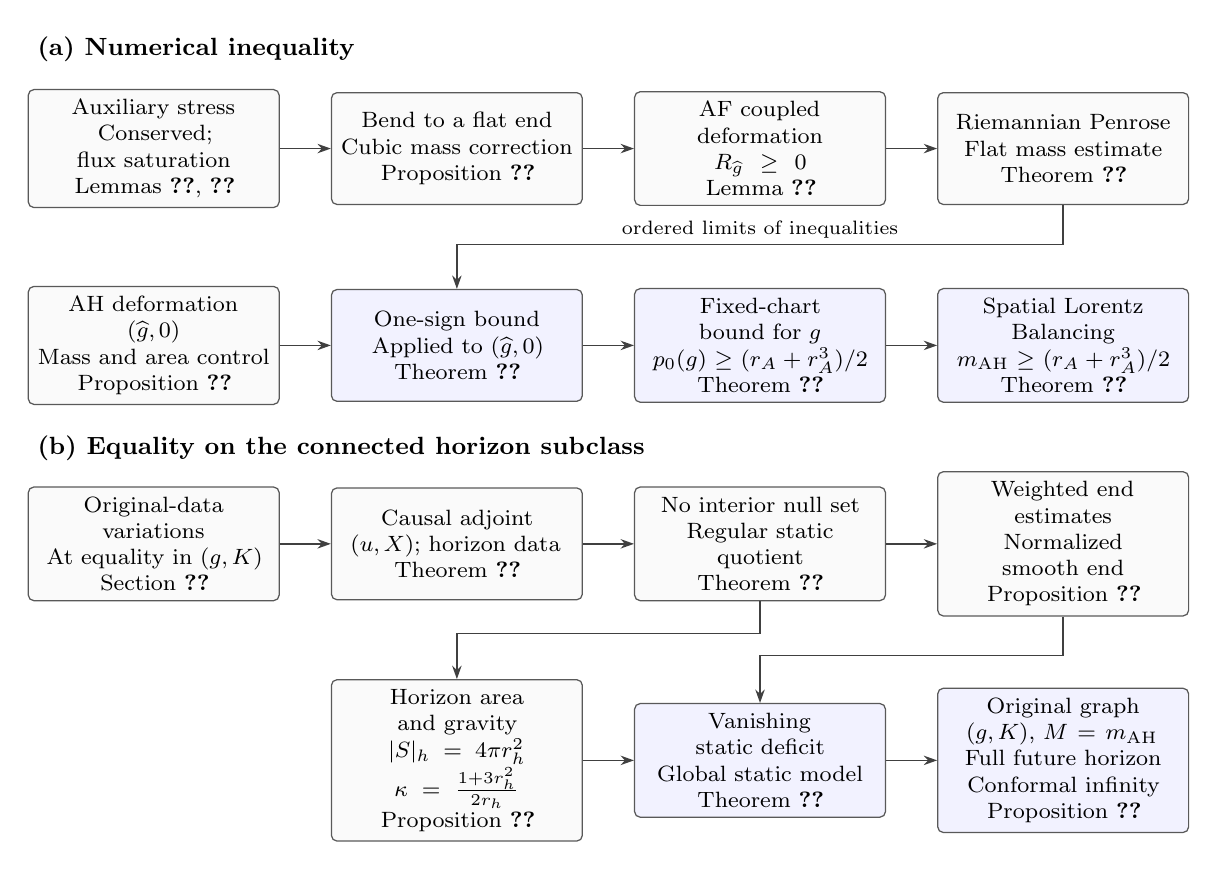
\begin{tikzpicture}[
  archbox/.style={draw=black!65, rounded corners=2pt, line width=.45pt,
    text width=2.94cm, minimum height=1.42cm, inner sep=3.5pt,
    align=center, font=\footnotesize},
  archstep/.style={archbox, fill=black!2},
  archresult/.style={archbox, fill=blue!5},
  archarrow/.style={-{Stealth[length=1.7mm,width=1.2mm]},
    draw=black!75, line width=.55pt},
  archheading/.style={anchor=west, font=\small\bfseries},
  archlabel/.style={font=\scriptsize, fill=white, inner sep=2pt}
]
\node[archheading] at (-1.60,1.26)
  {(a) Numerical inequality};
\node[archstep] (archstress) at (0,0)
  {Auxiliary stress\\ Conserved; flux saturation\\
   Lemmas~\ref{lem:str-flux-saturation}, \ref{lem:str-stress-identities}};
\node[archstep] (archbend) at (3.85,0)
  {Bend to a flat end\\ Cubic mass correction\\
   Proposition~\ref{prop:str-af-bending}};
\node[archstep] (archflat) at (7.70,0)
  {AF coupled deformation\\
   $R_{\widehat g}\ge0$\\
   Lemma~\ref{lem:fc-comparison-metric}};
\node[archstep] (archpenrose) at (11.55,0)
  {Riemannian Penrose\\ Flat mass estimate\\
   Theorem~\ref{thm:fc-mass-completion}};
\draw[archarrow] (archstress) -- (archbend);
\draw[archarrow] (archbend) -- (archflat);
\draw[archarrow] (archflat) -- (archpenrose);

\node[archstep] (archah) at (0,-2.50)
  {AH deformation\\
   $(\widehat g,0)$\\ Mass and area control\\
   Proposition~\ref{prop:ah-existence}};
\node[archresult] (archonesign) at (3.85,-2.50)
  {One-sign bound\\ Applied to $(\widehat g,0)$\\
   Theorem~\ref{thm:str-one-sign}};
\node[archresult] (archcomponent) at (7.70,-2.50)
  {Fixed-chart bound for $g$\\
   $p_0(g)\ge (r_A+r_A^3)/2$\\
   Theorem~\ref{thm:ah-component}};
\node[archresult] (archlorentz) at (11.55,-2.50)
  {Spatial Lorentz\\ Balancing\\
   $m_{\AH}\ge (r_A+r_A^3)/2$\\
   Theorem~\ref{thm:ah-invariant}};
\draw[archarrow] (archpenrose.south) -- (11.55,-1.22)
  -- node[archlabel,above] {ordered limits of inequalities}
  (3.85,-1.22) -- (archonesign.north);
\draw[archarrow] (archah) -- (archonesign);
\draw[archarrow] (archonesign) -- (archcomponent);
\draw[archarrow] (archcomponent) -- (archlorentz);

\node[archheading] at (-1.60,-3.80)
  {(b) Equality on the connected horizon subclass};
\node[archstep] (archvariations) at (0,-5.02)
  {Original-data variations\\ At equality in $(g,K)$\\
   Section~\ref{eq-section}};
\node[archstep] (archadjoint) at (3.85,-5.02)
  {Causal adjoint\\ $(u,X)$; horizon data\\
   Theorem~\ref{eq-causal-killing}};
\node[archstep] (archstatic) at (7.70,-5.02)
  {No interior null set\\ Regular static quotient\\
   Theorem~\ref{geo-static-quotient}};
\node[archstep] (archend) at (11.55,-5.02)
  {Weighted end estimates\\ Normalized smooth end\\
   Proposition~\ref{st-end-regularity}};
\draw[archarrow] (archvariations) -- (archadjoint);
\draw[archarrow] (archadjoint) -- (archstatic);
\draw[archarrow] (archstatic) -- (archend);

\node[archstep] (archhorizon) at (3.85,-7.77)
  {Horizon area and gravity\\
   $|S|_h=4\pi r_h^2$\\
   $\kappa=\frac{1+3r_h^2}{2r_h}$\\
   Proposition~\ref{st-base-equality}};
\node[archresult] (archhw) at (7.70,-7.77)
  {Vanishing static deficit\\ Global static model\\
   Theorem~\ref{hw-static-rigidity}};
\node[archresult] (archgraph) at (11.55,-7.77)
  {Original graph\\
   $(g,K)$, $M=m_{\AH}$\\ Full future horizon\\ Conformal infinity\\
   Proposition~\ref{emb-global}};
\draw[archarrow] (archstatic.south) -- (7.70,-6.16)
  -- (3.85,-6.16) -- (archhorizon.north);
\draw[archarrow] (archend.south) -- (11.55,-6.44)
  -- (7.70,-6.44) -- (archhw.north);
\draw[archarrow] (archhorizon) -- (archhw);
\draw[archarrow] (archhw) -- (archgraph);
\end{tikzpicture}
\caption{Dependencies of the two arguments. AF means asymptotically flat
and AH means asymptotically hyperbolic. Arrows indicate input to the
next step. In (a), the one-sign theorem is first proved by the upper
route and then applied to the AH comparison data; their mass covector
need not be timelike. Only the original mass covector is balanced.
In (b), equality and the numerical inequality give variations of the
original data. The normalized end and the inherited horizon area and
surface gravity jointly supply the static rigidity hypotheses.
Numerical area comparisons use full enclosing cuts.
The equality route uses no limit of the deformation metrics.}
\label{fig:proof-architecture}
\end{figure}


The local conformal AdS and asymptotically flat rigidity manuscripts
\cite{internalads,internalflat} motivate parts of the construction.
No theorem from either is assumed: the reused arguments and all changes
required by the present hypotheses are proved below. The public inputs
are invoked with their local geometry, regularity, asymptotic and
boundary hypotheses checked where they are used.

\section{Data, enclosing cuts, and the metric mass}\label{sec:setup}

We use the cosmological constant $\Lambda=-3$ and units $G=c=1$.
All initial data and boundaries are smooth. Norms at infinity are tensor
norms in the hyperbolic metric, rather than norms of coordinate components.

\begin{definition}[Initial-data exterior]\label{def:setup-data}
An initial-data exterior is a connected orientable three-manifold
$\Omega$ with nonempty compact smooth boundary $S$, a Riemannian metric
$g$, and a symmetric covariant tensor $K$. The metric space
$(\Omega,g)$, with its boundary included, is complete and has exactly one end.
Outside a compact set there is a chart $(r_0,\infty)\times\mathbb S^2$ with
\begin{equation}\label{eq:setup-background}
 b=\frac{dr^2}{1+r^2}+r^2\sigma,
 \qquad \eta=\operatorname{arsinh}r,
\end{equation}
where $\sigma$ is the unit round metric. For some $0<\alpha<1$ and
$3/2<\tau<3$, assume
\begin{equation}\label{eq:setup-decay}
 g-b\in C^{2,\alpha}_\tau,
 \qquad K\in C^{1,\alpha}_\tau.
\end{equation}
The space $C^{k,\alpha}_\tau$ controls $e^{\tau\eta}$ times the
$b$-norm of every covariant derivative through order $k$, and the
corresponding weighted H\"older seminorms on $b$-unit balls.
The noncosmological constraint densities are
\begin{equation}\label{eq:setup-constraints}
 16\pi\mu=R_g+6+(\tr_gK)^2-\lvert K\rvert_g^2,
 \qquad 8\pi J=\divg_g\bigl(K-(\tr_gK)g\bigr).
\end{equation}
We require
\begin{equation}\label{eq:setup-dec}
 \mu\ge\lvert J\rvert_g,
 \qquad
 \int_\Omega\sqrt{1+r^2}
       \bigl(\mu+\lvert J\rvert_g+\lvert K\rvert_g^2\bigr)
       \dd V_g<\infty,
\end{equation}
where the positive weight is extended smoothly over the compact part.
No restriction is placed on the compact topology, the number of boundary
components, or their genera.
\end{definition}

If $\nu$ is the normal toward the designated exterior and infinity, set
\begin{equation}\label{eq:setup-expansion}
 H=\divg_{S}\nu,
 \qquad \theta_+=H+\tr_{TS}K.
\end{equation}
The boundary hypothesis is $\theta_+\le0$ on every component of $S$,
with this same future sign. No condition on the other null expansion is
imposed. A spacetime realization uses
$K(Y,Z)=\overline g(\overline\nabla_Y n,Z)$ for the future unit normal $n$.
A surface with $\theta_+=0$ is a marginally outer trapped surface (MOTS).

\begin{definition}[Full enclosing cuts]\label{def:setup-cut}
An admissible exterior region is a connected smooth codimension-zero
submanifold with boundary $D\subset\Omega$, closed in $\Omega$, whose
interior lies in $\operatorname{int}\Omega$ and which contains the entire
sufficiently distant end. An admissible cut is its full compact intrinsic
boundary $\Gamma=\partial D$, assumed smoothly embedded and two-sided.
Coincidence with $S$, or with some of its components, is allowed. Define
\begin{equation}\label{eq:setup-area}
 A_{\min}(S;g)=\inf_{\Gamma}\Area_g(\Gamma),
 \qquad r_A=\sqrt{\frac{A_{\min}(S;g)}{4\pi}}.
\end{equation}
We omit $g$ when it is fixed. The competitor $D=\Omega$ has intrinsic
boundary $S$; it has area $\Area_g(S)$, not zero. Admissible cuts need not be
minimal or trapped, and may be disconnected.
\end{definition}

There is no extension across $S$ in this definition. An enclosing
minimization or trapped-region construction used below is always carried
out in the given exterior with $S$ as an obstacle or an actual boundary.
In particular, changing the exterior region requires comparison of the
entire cut, including any retained components of $S$.

\begin{definition}[Hyperbolic metric four-flux]\label{def:setup-mass}
Let $x_1,x_2,x_3$ be the coordinate functions on $\mathbb S^2$, and put
\begin{equation}\label{eq:setup-potentials}
 V_0=\sqrt{1+r^2},\qquad V_i=rx_i\quad(1\le i\le3).
\end{equation}
For $e=g-b$ and a static potential $V$, define the one-form
\begin{equation}\label{eq:setup-flux-form}
 \mathbb U_b(V,e)
 =V\bigl(\divg_b e-d\tr_be\bigr)
    +(\tr_be)dV-e(\nabla_bV,\cdot).
\end{equation}
The four mass components are
\begin{equation}\label{eq:setup-flux}
 p_a(g)=\frac1{16\pi}\lim_{R\to\infty}
   \int_{\{r=R\}}\mathbb U_b(V_a,e)(\nu_b)\dd A_b.
\end{equation}
The target class requires these limits to be finite and future timelike:
$p_0>\sqrt{p_1^2+p_2^2+p_3^2}$. Its mass is
\begin{equation}\label{eq:setup-invariant-mass}
 m_{\AH}(g)=\sqrt{p_0^2-p_1^2-p_2^2-p_3^2}.
\end{equation}
For auxiliary component estimates we do not impose timelikeness.
\end{definition}

The entries $p_i$ are spatial components of the metric mass covector.
They are not ADM momentum or angular momentum. This paper makes no
invariance assertion under arbitrary changes of asymptotic spacetime
slice. The asymptotic data are $(b,0)$ with $\Lambda=-3$.

\begin{lemma}[Flux convergence and spatial covariance]\label{lem:setup-mass-covariance}
The decay and integrability in Definition~\ref{def:setup-data} imply
convergence of the four integrals in Equation~\ref{eq:setup-flux}.
The same limits are obtained on any smooth exhaustion whose boundary
escapes every compact set. Under a fixed hyperbolic background isometry
the covector $p$ transforms by the corresponding Lorentz transformation.
It is invariant, with this transformation understood, under admissible
asymptotic spatial chart changes: both charts must satisfy the
tensor-decay and weighted-integrability conditions of
Definition~\ref{def:setup-data}. In particular, a future-timelike $p$
can be balanced by a spatial change of hyperbolic chart so that
$(p_0,p_1,p_2,p_3)=(m_{\AH},0,0,0)$.
\end{lemma}

\begin{proof}
Each $V_a$ satisfies $\Hess_bV_a=V_ab$ and $\Delta_bV_a=3V_a$.
The scalar curvature linearization at $b$ is
\[
 (DR)_b(e)=\divg_b\divg_be-\Delta_b\tr_be+2\tr_be.
\]
Differentiating Equation~\ref{eq:setup-flux-form} gives the exact identity
\begin{equation}\label{eq:setup-scalar-divergence}
 \divg_b\mathbb U_b(V_a,e)=V_a(DR)_b(e).
\end{equation}
In a sufficiently distant end write
$R_g+6=(DR)_b(e)+Q(e)$, where
\[
 \lvert Q(e)\rvert
 \le C\bigl(\lvert e\rvert\lvert\nabla_b^2e\rvert
                +\lvert\nabla_be\rvert^2+\lvert e\rvert^2\bigr).
\]
The right side is $O(e^{-2\tau\eta})$. Since
$|V_a|\le C e^\eta$ and $dV_b=O(e^{2\eta})d\eta dA_\sigma$,
the product $V_aQ$ is integrable precisely with the sufficient condition
$2\tau>3$. Moreover,
\[
 |R_g+6|\le16\pi\mu+4|K|_g^2,
\]
so $V_a(R_g+6)$ is integrable by Equation~\ref{eq:setup-dec} and the
uniform equivalence of $g$ and $b$ in the end. Equation~\ref{eq:setup-scalar-divergence}
and the divergence theorem now make the fluxes Cauchy. The difference
between their values on two escaping homologous cut boundaries is
bounded by the integral of this absolutely integrable divergence over
the intervening tail. This also proves the asserted exhaustion
independence for boundaries enclosing the same compact region.

In the hyperboloid model the four functions in
Equation~\ref{eq:setup-potentials} are its ambient coordinate functions.
A hyperbolic isometry therefore acts linearly on their span by a Lorentz
matrix. The flux expression is linear in $V$ and natural under a
background isometry. Its transformed coordinate spheres are an escaping
exhaustion, to which the preceding argument applies. This proves the
transformation law directly. The decay and weighted integrability remain
valid because a fixed hyperbolic isometry changes $\eta$ by a bounded
amount. The more general admissible spatial chart covariance is the
metric mass invariance Theorem of Chru\'sciel--Herzlich
\cite[Proposition~2.2 and Theorem~2.3]{chruscielherzlich2003}: its quadratic
decay threshold and weighted scalar-integrability hypotheses have just
been checked. Only the background-isometry case is needed to balance
the mass in the numerical proof. Finally, elementary Lorentz linear
algebra sends every future-timelike covector to its rest covector.
\end{proof}

\begin{remark}[Conformal normalization]\label{rem:setup-conformal-flux}
In three dimensions the linear flux for a pure conformal perturbation is
\begin{equation}\label{eq:setup-conformal-flux}
 \mathbb U_b(V,4t b)=-8(V\,dt-t\,dV).
\end{equation}
Indeed, $\tr_b(4tb)=12t$, $\divg_b(4tb)=4dt$, and the last two terms
of Equation~\ref{eq:setup-flux-form} sum to $8t\,dV$.
For example, if $t=O_1(r^{-s})$, $g-b=O_1(r^{-\tau})$,
$2s>3$, and $s+\tau>3$, then
\[
 e^{4t}g-g-4tb=O_1(r^{-2s})+O_1(r^{-s-\tau}).
\]
Its flux against each static potential is
$O(r^{3-2s})+O(r^{3-s-\tau})$, which tends to zero.
Thus Equation~\eqref{eq:setup-conformal-flux} gives the exact limiting
mass change whenever those limits exist; weighted scalar-curvature
integrability supplies their existence as above.
\end{remark}

\begin{definition}[Connected horizon subclass]\label{def:setup-horizon}
The horizon subclass consists of the preceding data with $S$ connected,
$\theta_+(S)=0$, and the following two properties. First, no compact
smooth embedded two-sided enclosing surface contained entirely in
$\operatorname{int}\Omega$, possibly disconnected and oriented on each
component toward infinity, has $\theta_+\le0$ everywhere. This is
outermostness. Second,
$\Area_g(S)\le\Area_g(\Gamma)$ for every full cut $\Gamma$.
This is outer area minimization, and gives
$A_{\min}(S)=\Area_g(S)$.
\end{definition}

\begin{lemma}[Schwarzschild--AdS normalization]\label{lem:setup-model-mass}
For $M>0$, let $F_M(r)=1+r^2-2M/r$ and let $r_h$ be its positive root.
The metric $g_M=F_M^{-1}dr^2+r^2\sigma$ on $[r_h,\infty)$, with
its smooth minimal-boundary interpretation, has
$(p_0,p_1,p_2,p_3)=(M,0,0,0)$. A full smooth spacelike cross-section
of the future horizon in the regular extension of
\begin{equation}\label{eq:setup-model-spacetime}
 \overline g_M=-F_M\,dt^2+F_M^{-1}dr^2+r^2\sigma
\end{equation}
has area $4\pi r_h^2$, and
$M=(r_h+r_h^3)/2$.
\end{lemma}

\begin{proof}
In the radial $b$-orthonormal frame, $g_M-b$ has just one entry,
\[
 q=\frac{2M}{rF_M},
\]
in the radial direction. Thus
$\mathbb U_b(V_0,g_M-b)(\nu_b)=2V_0\coth\eta\,q$.
The normalized integral is $M(1+r^2)/F_M$, which tends to $M$.
The three other integrals vanish by the zero spherical averages of
$x_i$. On the horizon the degenerate induced metric is the pullback of
$r_h^2\sigma$ from the space of null generators. A full spacelike
cross-section projects diffeomorphically onto that sphere and therefore
has its area. The relation between $M$ and $r_h$ follows from $F_M(r_h)=0$.
\end{proof}

Throughout the proof, estimates denoted by $O_j$ include derivatives
through order $j$ and the local H\"older control used in the relevant
elliptic estimate. Hyperbolic unit-ball estimates are distinguished from
asymptotic symbol estimates with derivatives $r\partial_r$ and
$\partial_\omega$. Preliminary approximation parameters are fixed before
subsequent deformation parameters. The final numerical limits are
limits of inequalities; no regular limiting deformation metric is
assumed in the equality argument.

\section{A saturating conserved stress and reduction to a flat end}
\label{sec:str-reduction}

Throughout this section, $A_g(S)$ denotes the full intrinsic-boundary
infimum $A_{\min}(S;g)$ of Definition~\ref{def:setup-cut}. All normals at
the original boundary point into the designated exterior. On an end,
$O_j(r^{-a})$ denotes a bound by $Cr^{-a}$ after at most $j$ derivatives
chosen from $r\partial_r$ and smooth angular vector fields. We write
$O_\infty$ when this holds for each fixed derivative order. Bounds in
physical weighted H\"older spaces are stated separately; they do not,
without further argument, assert bounds for all angular derivatives.

\begin{theorem}[The one-sign component inequality]
\label{thm:str-one-sign}
Let $(\Omega,g,K)$ satisfy Definition~\ref{def:setup-data}, and assume
$H+\tr_{TS}K\le0$ on every component of $S$, with the convention of
Equation~\eqref{eq:setup-expansion}. Suppose that $K$
is compactly supported and that one of the two tensors
\[
 K-(\tr_gK)g,\qquad -K+(\tr_gK)g
\]
is positive semidefinite throughout $\Omega$. In each fixed admissible
hyperbolic chart for which the metric fluxes exist,
\begin{equation}
 p_0(g)\geq \sqrt{\frac{A_g(S)}{16\pi}}
       +\frac12\left(\frac{A_g(S)}{4\pi}\right)^{3/2}.
 \label{eq:str-component-bound}
\end{equation}
This assertion does not require the flux covector to be timelike.
If that covector is future timelike, its Lorentz norm satisfies the
same lower bound.
\end{theorem}

The asymptotically flat result used in the proof is
Theorem~\ref{thm:fl-deformation}. Its required interface is the following:
a smooth exterior with one asymptotically Euclidean end, the full-cut
convention above, a strictly negative future boundary expansion, and
\begin{equation}
 \begin{split}
 R_q+(\tr_q B)^2-|B|_q^2
 -2\big|\operatorname{div}_q(B-(\tr_qB)q)\big|_q
     &\geq c(1+s)^{-3-\delta},\\
 q-\delta_{\mathrm{Eucl}}=O_\infty(s^{-1}),\qquad
 R_q&=O_\infty(s^{-3-\delta}),\\
 B=O_\infty(s^{-2}),\qquad \tr_qB&=0
 \quad\hbox{outside a compact set},
 \end{split}
 \label{eq:str-flat-interface}
\end{equation}
where $c>0$ and $0<\delta<1$, has ADM metric energy at least
$\sqrt{A_q(S)/(16\pi)}$. That theorem is proved in this manuscript; it
is not an additional premise.

\subsection{Conformal preparation with preservation of the component mass}

It is useful to fix the constraint normalization
\begin{equation}
 \mathcal H_g(K)=R_g+6+(\tr_gK)^2-|K|_g^2,
 \qquad
 \mathcal J_g(K)=\operatorname{div}_g(K-(\tr_gK)g).
 \label{eq:str-constraint-normalization}
\end{equation}
The dominant energy condition is $\mathcal H_g(K)\geq2|\mathcal J_g(K)|_g$.

\begin{lemma}[Preparation]
\label{lem:str-preparation}
Under the hypotheses of Theorem~\ref{thm:str-one-sign}, there are smooth
data $(g_i,K_i)$ on the same exterior, numbers $c_i>0$, and a fixed
$0<\delta<1$ such that:
\begin{enumerate}[label=(\roman*)]
\item $K_i$ is compactly supported, with the same global stress sign as
      $K$, and its future boundary expansion has the original weak sign;
\item $\mathcal H_{g_i}(K_i)-2|\mathcal J_{g_i}(K_i)|_{g_i}
      \geq c_i(1+r)^{-3-\delta}$, with $r$ smoothly extended over a
      compact region;
\item $g_i=e^{4v_i}b$ on an exact tail, where
\begin{equation}
 v_i=r^{-3}v_{3,i}(\omega)-d_{0,i}r^{-3-\delta}
             +O_\infty(r^{-4}),
 \qquad d_{0,i}>0,
 \label{eq:str-prepared-expansion}
\end{equation}
and $v_{3,i}$ is smooth;
\item for a fixed $\beta>3/2$, $g_i\to g$ and $K_i\to K$ in physical
      weighted $C^{2,\alpha'}_\beta$ and $C^{1,\alpha'}_\beta$ norms,
      respectively, with any fixed sufficiently small $\alpha'>0$;
\item $p_a(g_i)\to p_a(g)$ for all four metric fluxes and
      $A_{g_i}(S)\to A_g(S)$.
\end{enumerate}
When $K=0$, one may take $K_i=0$. A minimal boundary remains minimal,
and the convergence on fixed compact subsets is smooth if the original
metric is smooth there.
\end{lemma}

\begin{proof}
Choose
\begin{equation}
 \frac32<\beta<\min\{\tau,3\},\qquad
 0<\delta<\min\{2\beta-3,1\},\qquad
 \eta_R=R^{\beta-\tau}.
 \label{eq:str-preparation-parameters}
\end{equation}
Take $R$ beyond the support of $K$ and a fixed cutoff
$\chi_R=\chi(r/R)$, equal to one for $r\leq R$ and zero for $r\geq2R$.
Set $q_R=b+\chi_R(g-b)$ on the end and $q_R=g$ elsewhere. For large
$R$ this is positive definite. The curvature cutoff error
\[
 E_R=\frac18\{\chi_R(R_g+6)-(R_{q_R}+6)\}
\]
is supported in $R\leq r\leq2R$ and satisfies
\begin{equation}
 \|E_R\|_{C^{0,\alpha'}_\beta}\leq C\eta_R.
 \label{eq:str-cutoff-source}
\end{equation}
Indeed, the scalar-curvature formula uses two derivatives of the
metric, physical derivatives of $\chi(r/R)$ are uniformly bounded on
this annulus, and every term contains $g-b$ or one of its first two
physical derivatives. The quadratic terms decay faster. The metrics
$q_R$ have uniform bounded-geometry coordinate estimates of the orders
used here.

Choose a nonnegative smooth compactly supported function $D\geq|K|_g$,
with support in the region where $q_R=g$, and a smooth positive $w_0$
equal to $r^{-3-\delta}$ far out. We solve
\begin{equation}
 \begin{cases}
 (-\Delta_{q_R}+3)v
 =D\sqrt{\eta_R^2+|dv|_{q_R}^2}+E_R+\eta_Rw_0,\\
 \partial_\nu v=0\quad\hbox{on }S,\qquad v\longrightarrow0
 \quad\hbox{at infinity}.
 \end{cases}
 \label{eq:str-preparation-equation}
\end{equation}
Here the sign of the normal in the homogeneous Neumann condition is
immaterial.

We give the existence and uniform estimates. On a finite truncation
put $v=0$ on its outer sphere, and multiply the entire right side of
Equation~\eqref{eq:str-preparation-equation} by $\lambda\in[0,1]$.
Write its gradient term as $W\cdot dv+F_D$, where $|W|\leq D$ and
$0\leq F_D\leq D\eta_R$; for example this follows from
\[
 \sqrt{\eta_R^2+|dv|^2}
 =\frac{|dv|^2}{\sqrt{\eta_R^2+|dv|^2}}
   +\frac{\eta_R^2}{\sqrt{\eta_R^2+|dv|^2}}.
\]
The maximum principle for $-\Delta-W\cdot d+3$, with the indicated
mixed boundary conditions, bounds $|v|$ by $C\eta_R$. Outside a fixed
sphere containing $\supp D$, the radial function $r^{-\beta}$ satisfies
\[
 (-\Delta_{q_R}+3)r^{-\beta}
 =\{(3-\beta)(\beta+1)+o(1)\}r^{-\beta}
 \geq c_\beta r^{-\beta}
\]
uniformly in $R$. Comparison using Equation~\eqref{eq:str-cutoff-source}
therefore sharpens the bound to
\begin{equation}
 |v|\leq C\eta_R(1+r)^{-\beta}.
 \label{eq:str-v-height}
\end{equation}
The boundary constants in these comparisons are independent of the
outer truncation.

For completeness, the required derivative bounds follow from scalar
elliptic estimates without any coupled-system assumption. Divide the
equation by $\eta_R$ and write $u=v/\eta_R$. Its gradient dependence is
$D\sqrt{1+|du|^2}$, with uniformly bounded first derivative in $du$.
Local $W^{2,p}$ estimates on physical balls, the corresponding Neumann
or Dirichlet half-ball estimates, and first-derivative interpolation
give a bound for $u$ in $W^{2,p}$ on smaller patches in terms of its
already bounded height and the source $E_R/\eta_R+w_0$. One can see the
absorption directly by applying the estimate to nested cutoffs and
using
\[
 \|du\|_{L^p}\leq\varepsilon\|u\|_{W^{2,p}}
                       +C_\varepsilon\|u\|_{L^p}.
\]
Choose $p>3$ sufficiently large. Sobolev embedding makes $du$ H\"older,
and the scalar Schauder estimate then gives $C^{2,\alpha'}$ control.
On the end the same argument is applied after multiplication by the
local weight, which is comparable on every physical unit patch.
Thus
\begin{equation}
 \|v\|_{C^{2,\alpha'}_\beta}\leq C\eta_R.
 \label{eq:str-v-estimate}
\end{equation}
Lemma~\ref{lem:linear-separated-faces} supplies these scalar estimates
and the finite-domain inverse. Its local reflection argument permits
bounded drift, and its Schauder step is applied to the original
one-sided equation after the gradient becomes H\"older.
The ellipticity, boundary smoothness, source regularity and
gradient-growth hypotheses have just been specified. The linearization of the finite-domain equation is
\[
 -\Delta_{q_R}+3-
 \lambda D\frac{\langle dv,d(\,\cdot\,)\rangle}
                    {\sqrt{\eta_R^2+|dv|^2}}.
\]
Its kernel vanishes by the same maximum principle. Its index is zero
by continuation of the bounded drift from zero. It is therefore an
isomorphism with these boundary conditions. The a priori bounds close
the continuation from $\lambda=0$ to $1$. Exhaustion, the uniform
estimates, and a diagonal subsequence give a smooth solution of
Equation~\eqref{eq:str-preparation-equation}.

On its exact hyperbolic tail, this solution satisfies
$(-\Delta_b+3)v=\eta_Rr^{-3-\delta}$. Rotations commute with the
operator and annihilate this radial source. Applying difference
quotients, comparison by $r^{-\beta'}$ for any fixed $\beta'<3$, and
local elliptic estimates gives the same decay for all fixed angular
derivative orders. The hyperbolic Laplacian is
\[
 \Delta_b=(1+r^2)\partial_r^2+(2/r+3r)\partial_r
                         +r^{-2}\Delta_\sigma.
\]
Consequently, for $\beta'$ sufficiently close to $3$,
\[
 (-r^2\partial_r^2-3r\partial_r+3)v
 =\eta_Rr^{-3-\delta}+O_\infty(r^{-2-\beta'}).
\]
Variation of constants for the two Euler solutions $r$ and $r^{-3}$,
with the growing solution excluded by decay, yields
\[
 v=r^{-3}v_3(\omega)
   -\frac{\eta_R}{\delta(4+\delta)}r^{-3-\delta}
   +O_\infty(r^{-4}).
\]
Angular difference quotients give a smooth $v_3$, and differentiating
the radial equation gives the stated symbol estimates. In particular
$d_0=\eta_R/[\delta(4+\delta)]>0$.

Define
\[
 \widetilde g=e^{4v}q_R,\qquad \widetilde K=e^{2v}K.
\]
The stress transforms as
$\widetilde K-(\tr_{\widetilde g}\widetilde K)\widetilde g
=e^{2v}(K-(\tr_{q_R}K)q_R)$, so its sign is retained. The conformal
boundary formula is
\[
 H_{\widetilde g}+\tr_T\widetilde K
 =e^{-2v}(H_{q_R}+\tr_TK+4\partial_\nu v),
\]
which preserves the original expansion sign. The scalar and divergence
formulas are
\begin{align}
 e^{4v}\mathcal H_{\widetilde g}(\widetilde K)
 &=\mathcal H_{q_R}(K)+6(e^{4v}-1)
                       -8\Delta_{q_R}v-8|dv|_{q_R}^2,
 \label{eq:str-conformal-hamiltonian}\\
 \mathcal J_{\widetilde g}(\widetilde K)
 &=e^{-2v}\{\mathcal J_{q_R}(K)+4K(\nabla v,\cdot)\}.
 \label{eq:str-conformal-momentum}
\end{align}
The momentum norm in the second formula gains a further $e^{-2v}$.
Substituting Equation~\eqref{eq:str-preparation-equation}, using
$D\sqrt{\eta_R^2+|dv|^2}\geq |K||dv|$, and using the original DEC on
the support of $K$ and its scalar version outside that support, gives
\[
 e^{4v}\{\mathcal H_{\widetilde g}(\widetilde K)
                 -2|\mathcal J_{\widetilde g}(\widetilde K)|\}
 \geq8\eta_Rw_0-8|dv|^2+6(e^{4v}-1)-24v.
\]
The last two terms are nonnegative. Equation~\eqref{eq:str-v-estimate}
and $2\beta>3+\delta$ give
$|dv|^2\leq C\eta_R^2(1+r)^{-3-\delta}$. For large $R$ the required
strict margin follows.

Uniform bilinear convergence of $\widetilde g$ to $g$ gives convergence
of every full-cut infimum: if
$(1-\epsilon)g\leq\widetilde g\leq(1+\epsilon)g$, the same factors
bound all two-dimensional areas, hence their infima. To verify mass
convergence, observe outside $\supp D$ that
\[
 e^{4v}(R_{\widetilde g}+6)
 =\chi_R(R_g+6)+8\eta_Rw_0+O(v^2+|dv|^2).
\]
The weighted integrals of the right side on distant tails are uniformly
small. The scalar-linearization divergence formula in
Lemma~\ref{lem:setup-mass-covariance} has quadratic remainder bounded
by $C V_0r^{-2\beta}$, whose integral is finite because $\beta>3/2$.
Compare the fluxes first on a fixed sphere, where local convergence
applies, and then bound both tails by these integrals. Since
$|V_a|\leq V_0$, this proves convergence for all four fluxes.
Finally, for $K=0$, $D=0$ and the correction equation is linear on
each fixed compact subset for all sufficiently large $R$. Differentiated
local estimates prove the asserted smooth convergence. Relabeling a
sequence $R\to\infty$ proves the lemma.
\end{proof}

\subsection{Full-cut comparison under addition of a short collar}

\begin{lemma}[A collar with almost unchanged cut infimum]
\label{lem:str-added-collar}
Let $(\Omega,g)$ be smooth up to its compact boundary. For every
sufficiently small $\varepsilon>0$ there is an enlarged exterior
$(\Omega_\varepsilon,g_\varepsilon)$, obtained by adding a collar on
the inner side of every boundary component, which agrees with $g$ on
$\Omega$, has a product metric near its new boundary, and satisfies
\begin{equation}
 A_{g_\varepsilon}(\partial\Omega_\varepsilon)
 \geq(1-o(1))A_g(S)\qquad(\varepsilon\downarrow0).
 \label{eq:str-collar-area}
\end{equation}
No constraint inequality on the added collar is required.
\end{lemma}

\begin{proof}
Use disjoint Gaussian collars $[0,L]\times S_j$ with metric
$dx^2+q_j(x)$, where $L>0$ is fixed. Extend $q_j$ smoothly to
$[-\varepsilon,0]$. Since $q_j(x)=q_j(0)+O(\varepsilon)$ there, a
cutoff to the constant $q_j(-\varepsilon)$ near $-\varepsilon$ changes
only the metric values by $O(\varepsilon)$; derivatives may depend on
$\varepsilon$. Choose a smooth map
$F_\varepsilon:[-\varepsilon,L]\to[0,L]$ equal to the identity near
$L$, mapping endpoints to endpoints, and satisfying
$F_\varepsilon-x=O(\varepsilon)$ and
$F_\varepsilon'=1+O(\varepsilon/L)$. Its product with the identity on
$S_j$, extended by the identity elsewhere, is a diffeomorphism
$\Phi_\varepsilon:\Omega_\varepsilon\to\Omega$ with
\[
 (1-o(1))g_\varepsilon\leq\Phi_\varepsilon^*g
                       \leq(1+o(1))g_\varepsilon.
\]
This diffeomorphism maps a connected exterior submanifold and its
entire intrinsic boundary to another of the same type. Applying the
area comparison to every such cut proves
Equation~\eqref{eq:str-collar-area}. The new product face has mean
curvature zero.
\end{proof}

\subsection{The nonlinear Dirichlet problem}
\label{str-pde-section}

For $s\geq0$, define $t(s)\in[0,1)$ by
\begin{equation}\label{str-pde-law}
 s^2=\frac{t}{1-t^{3/2}},\qquad
 b(s)=\frac{s t'(s)}{t(s)}
      =\frac{4(1-t^{3/2})}{2+t^{3/2}}.
\end{equation}
The limiting value of $b$ at zero is $2$. Set
$a(s)=t(s)/s^2$, with $a(0)=1$. Then
\begin{equation}\label{str-pde-law-limits}
\begin{gathered}
 a+s^3a^{3/2}=1,\\
 a=1-s^3+O(s^6),\qquad t=s^2-s^5+O(s^8)
       \qquad(s\downarrow0),\\
 b s^2=\frac{4t}{2+t^{3/2}}\longrightarrow\frac43
       \qquad(s\longrightarrow\infty).
\end{gathered}
\end{equation}
In particular, $0<b\leq2$ and
$\inf_{s\geq0}b(s)(1+s^2)>0$.
The vector $t(|df|_g)\nabla_g f/|df|_g$ is defined to be zero at
critical points. Its continuous dependence on $df$ will always be
understood in this sense.

\begin{theorem}[Fixed-height stress potential]\label{thm:str-stress-dirichlet}
\label{str-pde-fixed-height}
Let $(X,g)$ be a connected smooth complete three-dimensional exterior
with compact smooth nonempty boundary, exactly one end, and a smooth
metric up to its boundary. Let $H_{\partial X}\leq0$, for the normal
pointing into $X$. Suppose that on the end, with $z=r^{-1}$,
\begin{equation}\label{str-pde-prepared-end}
 g=z^{-2}\bar g,\qquad
 \bar g=e^{4v}\left(\frac{dz^2}{1+z^2}+\sigma\right),\qquad
 v=z^3v_3(\omega)-d z^{3+\delta}+O_\infty(z^4),
\end{equation}
where $v_3$ is smooth, $0<\delta<1$, and the remainder and its
tangential derivatives satisfy the indicated symbol estimates.
For every $D>0$ there is a unique bounded weak solution
\begin{equation}\label{str-pde-dirichlet}
 \divg_g\left(t(|df|_g)\frac{\nabla_g f}{|df|_g}\right)=0,
 \qquad f|_{\partial X}=D,\qquad \lim_{r\to\infty}f=0.
\end{equation}
It satisfies $0<f<D$ in the interior, has bounded physical gradient,
belongs to $C^{1,\theta}$ on compact subsets including the finite
boundary for some $\theta>0$, and is smooth wherever $df\ne0$.
On a collar of conformal infinity it is noncritical and
\begin{equation}\label{str-pde-end-expansion}
\begin{gathered}
 f=z C_f(\omega)+R_f,\qquad C_f\in C^\infty(\mathbb S^2),
 \qquad C_f>0,\\
 |(z\partial_z)^j\partial_\omega^\nu R_f|
 \leq C_{j,\nu}z^2\quad(0\leq j\leq2).
\end{gathered}
\end{equation}
The constants can depend on $D$ and the fixed geometry. In particular,
\begin{equation}\label{str-pde-end-flux}
 \begin{gathered}
 |df|_g=zC_f+O(z^2),\qquad
 t(|df|_g)=z^2C_f^2+O(z^3),\\
 -\lim_{r\to\infty}\int_{\{r=\mathrm{const}\}}
 t(|df|_g)\left\langle\frac{\nabla_g f}{|df|_g},\nu_g\right\rangle
 dA_g=\int_{\mathbb S^2}C_f^2\,dA_\sigma .
 \end{gathered}
\end{equation}
\end{theorem}

We give the a priori estimates and the existence argument separately.
In what follows, constants are independent of the outer truncation
and of the regularization parameter, unless stated otherwise.

\begin{lemma}[Regularization and the public regularity input]
\label{str-pde-regularity-input}
For sufficiently small $h>0$, choose a smooth $b_h$ equal to $1$ on
$[0,h/2]$, equal to $b$ on $[2h,\infty)$, and between $1$ and $2$ on
the intervening interval. Define $t_h$ by
$s t_h'/t_h=b_h$ and $t_h(2h)=t(2h)$. For each fixed $M<\infty$,
\begin{equation}\label{str-pde-regularized-structure}
 c_M(h+s)s\leq t_h(s)\leq C_M(h+s)s,\qquad
 c_M(h+s)\leq t_h'(s)\leq C_M(h+s)
 \quad(0\leq s\leq M).
\end{equation}
Here $t_h(s)/s$ is constant near zero, so the regularized vector
field is smooth at the zero covector. On coordinate patches with
uniformly controlled metric and first derivatives, its density
\[
 A_h^i(x,p)=\sqrt{\det g}\,\frac{t_h(|p|_g)}{|p|_g}g^{ij}p_j
\]
obeys, for $|p|\leq M$,
\begin{equation}\label{str-pde-density-structure}
 \begin{split}
 \lambda_M(h^2+|p|^2)^{1/2}|\zeta|^2
 &\leq D_pA_h[\zeta,\zeta],\qquad
 |D_pA_h|\leq\Lambda_M(h^2+|p|^2)^{1/2},\\
 |A_h|+|\partial_x A_h|&\leq C_M(h+|p|)|p|.
 \end{split}
\end{equation}
Once an a priori gradient bound $M$ has been established, the field
can be extended for $|p|>M$ to satisfy these inequalities globally,
with possibly changed constants independent of $h$.

Consequently bounded weak solutions with this gradient bound have
local $C^{1,\theta}$ estimates, including Dirichlet boundary patches,
uniformly in $h$. On interior unit patches for $h=0$, the estimate
can be normalized to give
\begin{equation}\label{str-pde-oscillation-gradient}
 \sup_{B_{1/2}}|df|_g\leq C\operatorname{osc}_{B_1} f,
\end{equation}
provided the same fixed extension and the same structural constants
apply on the patch. Smooth boundary data on finite boundary patches
are allowed.
\end{lemma}
\begin{proof}
Below $h/2$ the normalization gives $t_h(s)=c_hs$ with
$c_h\asymp h$. On the transition interval $s\asymp h$,
$t_h\asymp h^2$, and $b_h\in[1,2]$. Above it the inequalities
follow from $t/s^2>0$ and $b>0$ on a bounded interval.
The radial and tangential eigenvalues of the covector derivative
are $t_h'$ and $t_h/s$. Metric differentiation costs at most a
constant times $|p|_g$ in differentiating $|p|_g$, and
$s t_h'=b_h t_h\leq2t_h$. These facts prove
\eqref{str-pde-density-structure}.
For example, outside a slightly larger bounded-gradient interval
one may interpolate the logarithmic derivative to $2$ and then
continue by a quadratic flux law. Positive lower and upper bounds
for that logarithmic derivative give the required global extension.
This extension is used only after the gradient bound; it is not an
existence argument for the saturating law.

We specify the hypotheses of the regularity theorem.
For $-\partial_i A^i(x,u,Du)=B(x,u,Du)$ on a $C^{1,\alpha}$
domain, Appendix Theorem A.1 of \cite{porrettaveron2009} permits
\[
 \lambda(\mu^2+|p|^2)^{(p_0-2)/2}I
 \leq D_pA\leq
 \Lambda(\mu^2+|p|^2)^{(p_0-2)/2}I,
\]
an analogous bound for $|D_pA|$, and the spatial and scalar
continuity condition
\[
 |A(x,s,p)-A(y,t,p)|
 \leq C(1+|p|^{p_0-2}+|p|^{p_0-1})
       (|x-y|^\alpha+|s-t|^\alpha),
 \qquad |B|\leq C(1+|p|^{p_0}).
\]
For bounded weak solutions it yields a H\"older continuous gradient
up to a $C^{1,\alpha}$ Dirichlet boundary; the same local argument
gives the interior estimate. We apply it with $p_0=3$, $\mu=h$,
no scalar dependence, and $B=0$. The metric bounds and
\eqref{str-pde-density-structure} verify every displayed condition;
constants on a fixed height and gradient range are uniform in $h$.
At a finite Dirichlet face the datum is constant; subtracting that
constant reduces a boundary patch to the homogeneous theorem.
The finitely many smooth boundary components are disjoint, so
these patches can be chosen separately. At conformal infinity
the datum is already zero.
The interior gradient estimates originate in
\cite{tolksdorf1984}, and the frozen boundary estimate used in the
proof is the boundary regularity estimate of \cite{lieberman1988}.
We use the stated Appendix theorem as the precise boundary input.

For completeness, normalization removes any additive constant in
the interior gradient bound. Extend the unregularized density with
$D_pA\asymp|p|$ and $|\partial_xA|\leq C|p|^2$. If
$m=\operatorname{osc}_{B_1}f>0$, subtract the infimum and put
$u=f/m$. The equation for $u$ has density
$A_m(x,p)=m^{-2}A(x,mp)$, whose structural constants do not depend
on $m$. Since $0\leq u\leq1$, the local gradient estimate for $u$
is uniform. Multiplication by $m$ proves
\eqref{str-pde-oscillation-gradient}. The case $m=0$ is immediate.
\end{proof}

\begin{lemma}[Boundary barriers and global gradient bound]
\label{str-pde-global-gradient}
Let $f$ be a classical regularized solution on a truncation $X_R$,
with boundary values $D'$ at the finite boundary and zero at
$r=R$, where $0\leq D'\leq D$. Then
\begin{equation}\label{str-pde-global-bounds}
 0\leq f\leq D,\qquad |df|_g\leq M_D,
 \qquad f\leq C_Dr^{-\xi}\quad(r\geq r_1),
\end{equation}
for any fixed $0<\xi<1$ and suitable $r_1,C_D,M_D$ independent
of small $h$ and sufficiently large $R$.
\end{lemma}
\begin{proof}
At a noncritical point put $s=|df|_g$, $e=\nabla f/s$, and
\[
 Lf=A^{ij}\nabla_i\nabla_jf=0,
 \qquad A=g^{-1}+(b_h-1)e\otimes e.
\]
The maximum principle gives the height bound.
Let $d$ be the inward distance from the finite boundary. Its level
sets have mean curvature $H(d)=\Delta_g d\leq C d$ in a fixed
collar, since $H(0)\leq0$. Consider
\[
 \underline f=D'-\gamma(d),\qquad
 \gamma'(d)=\frac{c}{\sqrt{d^2+d_*^2}}.
\]
The radial operator on this function is
\begin{equation}\label{str-pde-inner-barrier}
 L\underline f
 =\gamma'\left(\frac{b_h(\gamma')d}{d^2+d_*^2}-H(d)\right).
\end{equation}
Uniformly in $h$, $b_h(s)(1+s^2)\geq c_0>0$, and hence
\[
 \frac{b_h(\gamma')}{d^2+d_*^2}
 \geq\frac{c_0}{d^2+d_*^2+c^2}.
\]
Choose the collar length $\ell$ and $c>0$ small first; then choose
$d_*>0$ sufficiently small. The last bound makes
\eqref{str-pde-inner-barrier} nonnegative on $[0,\ell]$, while
$\gamma(\ell)=c\operatorname{arsinh}(\ell/d_*)\geq D$.
Comparison with $\underline f$ and the constant upper barrier
gives a uniform finite-boundary gradient bound $c/d_*$.

On the end, for $F(r)=r^{-\xi}$, the leading radial operator is
$\xi(b_h\xi-2)r^{-\xi}$, with relative error tending to zero
uniformly for $0<b_h\leq2$. Thus $F$ is a strict supersolution
beyond a fixed sphere, uniformly in any positive multiple of $F$.
Comparison with
$K_D(r^{-\xi}-R^{-\xi})$ gives both the last estimate in
\eqref{str-pde-global-bounds} and the outer-boundary gradient
bound. Choose $K_D$ at the fixed inner sphere before sending
$R$ to infinity; for $R$ at least twice its radius the required
$K_D$ is uniform.

It remains to exclude a large interior gradient. The following
calculation is for $s\geq s_0$, where $b_h=b$.
Writing $x=t^{3/2}$ gives
\[
 b+s b'=b\left(1-\frac{18x}{(2+x)^2}\right).
\]
Thus, for fixed sufficiently large $s_0$, $b<1$ and $b+s b'<0$.
At a point with first frame vector $e$, differentiating $Lf=0$
and commuting covariant derivatives yields the exact identity
\begin{equation}\label{str-pde-log-gradient}
\begin{aligned}
 L\log s
 &=\frac{1}{s^2}\Bigl(
 |\Hess f|_{e^\perp\times e^\perp}^2
 +(1-b)|\Hess f(e,\cdot)|_{e^\perp}^2\Bigr)\\
 &\quad-\frac{b+s b'}{s^2}\Hess f(e,e)^2+\Ric_g(e,e).
\end{aligned}
\end{equation}
To see the coefficients, differentiate $A$ in the $e$ direction:
its contraction with $\Hess f$ is
$b'\Hess f(e,e)^2+
 2(b-1)s^{-1}|\Hess f(e,\cdot)|_{e^\perp}^2$.
The two derivatives of $\log s$ then leave exactly the three
quadratic terms displayed. In the curvature commutator the
additional $(b-1)e\otimes e$ term vanishes by antisymmetry, leaving
$\Ric(e,e)$.
The Ricci curvature is bounded below on the whole exterior, so
$L\log s\geq-C$. Moreover $L(f^2)=2b s^2$ and
$\inf_{s\geq s_0}b s^2>0$. Choose $c_1$ so large that
\[
 L(\log s+c_1f^2)>0\qquad(s\geq s_0).
\]
An interior maximum in this range is impossible. The two boundary
gradient bounds and $0\leq f\leq D$ therefore bound the maximum
of $\log s+c_1f^2$, and then $s$, everywhere. At a critical point
$\log s=-\infty$, so such points cause no difficulty in this
maximum argument.
\end{proof}

\begin{proof}[Existence, uniqueness, and finite-boundary regularity in
Theorem~\ref{str-pde-fixed-height}]
Fix $h>0$ and a finite smooth truncation. Use the homotopy of
boundary values $\lambda D$, $0\leq\lambda\leq1$, for the original
regularized saturating equation. At $\lambda=0$ the zero solution
exists. For fixed $h$ and on the gradient range of
Lemma~\ref{str-pde-global-gradient}, the operator is uniformly
elliptic and smooth in the covector. Its linearization has no
zeroth-order term, is invertible with homogeneous Dirichlet data
by the maximum principle and linear elliptic solvability, and
gives openness. For closedness, first apply
Lemma~\ref{str-pde-regularity-input} using the already established
gradient bound. Its extension agrees with the original flux on
every solution. This gives a common $C^{1,\theta}$ bound; the
ordinary uniformly elliptic Schauder estimates for this fixed
$h$ then give $C^{2,\theta'}$ bounds and the required compactness.
The continuity method therefore reaches $\lambda=1$; the linear
Dirichlet solvability and Schauder estimates used here follow from
Lemma~\ref{lem:linear-separated-faces}, including its general-principal
all-Dirichlet conclusion.
No uniform ellipticity as $h\downarrow0$ is asserted at this step.

Now use the estimates that are uniform in $h$ and in the outer
truncation. On every fixed interior or finite-boundary patch,
the $C^{1,\theta}$ estimates permit a diagonal $C^1$ limit as
$h\downarrow0$ and $R\to\infty$. The fluxes converge locally
uniformly, so the weak equation and finite Dirichlet trace pass
to the limit. The common bound $C_Dr^{-\xi}$ gives the zero
limiting value at infinity. Interior elliptic bootstrap applies
on every set where $df\ne0$.

The unregularized flux is strictly monotone in the covector:
its radial potential has derivative $t(s)$, with $t'>0$ for
$s>0$. For two solutions $f_1,f_2$, test the difference of the
weak equations by $(f_1-f_2-\varepsilon)_+$. This test has compact
support, since both functions tend uniformly to zero at infinity,
and has zero trace on the finite boundary. Strict monotonicity
forces its gradient to vanish. It is therefore zero; letting
$\varepsilon\downarrow0$ proves $f_1\leq f_2$, and interchanging
the solutions proves uniqueness. The same comparison proves
monotonicity in $D$.
Positivity can be propagated by a direct local comparison.
On a compact geodesic annulus $r_0<\varrho<r_1$ lying below
the injectivity radius, take
$w=A(e^{-k\varrho^2}-e^{-kr_1^2})$. Its radial operator is
$b w''+w'\Delta_g\varrho$. First choose $k$ so large that
$b_0(2k\varrho-1/\varrho)\geq\Delta_g\varrho$ on the annulus,
where $b_0=\min_{0\leq s\leq1}b(s)>0$. Then take $A>0$
small enough that $|dw|\leq1$ and the inner boundary value
of $w$ is below a given positive minimum of $f$. Since
$w''/(-w')=2k\varrho-1/\varrho$, this is a positive
subsolution, zero at the outer sphere. Weak comparison
propagates positivity from the inner ball to the larger
ball. The finite-boundary barrier supplies an initial
positive collar; a finite chain of interior balls along
any path proves $f>0$ throughout the connected interior.
Apply the same argument to $D-f$, which solves the same
odd-flux equation and is positive near infinity, to obtain
$f<D$. This completes the asserted existence and
finite-boundary statements.
\end{proof}

\subsection{The conformal boundary and its expansion}

\begin{lemma}[Linear height and physical-gradient bounds at infinity]
\label{str-pde-linear-end-bounds}
For the solution in Theorem~\ref{str-pde-fixed-height} there are
$c,C,Q>0$ and a collar $0<z<z_0$ such that
\begin{equation}\label{str-pde-linear-bounds}
 cz\leq f\leq Cz,\qquad |df|_g\leq Qz.
\end{equation}
These constants can be chosen uniformly for a family whenever
the coarse bounds $f\leq C_0z^\xi$, a positive lower bound on one
fixed inner sphere, local physical gradient bounds, and the
compact metric bounds used in the proof are uniform.
\end{lemma}
\begin{proof}
There is a useful radial identity that also applies to the
families considered below. For $g=z^{-2}\bar g$, put
$u=|dz|_{\bar g}^2$ and
$\bar e=\nabla_{\bar g}z/\sqrt u$. If $F'>0$, the operator on
$F(z)$, divided by $z^2u$, is
\begin{equation}\label{str-pde-compact-radial}
 bF''+\left(\frac{b-2}{z}+E\right)F',\qquad
 E=\frac{\Delta_{\bar g}z+(b-1)\Hess_{\bar g}z(\bar e,\bar e)}u,
 \qquad b=b(z\sqrt u F').
\end{equation}
Indeed
$\Hess_g z=\Hess_{\bar g}z+
 2z^{-1}dz\otimes dz-z^{-1}u\bar g$ and
$\Delta_g z=z^2\Delta_{\bar g}z-zu$.
For \eqref{str-pde-prepared-end},
\[
 E=\frac{b z}{1+z^2}-2(b-2)v_z=O(z)
\]
uniformly for $0<b\leq2$. More generally, if
$\bar g-h_0=O_2(z^\beta)$ with
$h_0=(1+z^2)^{-1}dz^2+\sigma$ and $\beta>1$, then
$E=O(z)+O(z^{\beta-1})$, again uniformly in $b$.

Choose $F_+(z)=A(z-c_2z^2)$ with a fixed $c_2>0$.
The term $(b-2)F_+'/z$ is nonpositive. Make $z_0$ small
and take $A$ sufficiently large for $F_+(z_0)\geq f(z_0,\cdot)$.
The order of these choices can be made consistent with small
physical slope: the coarse bound allows
$A=2C_0z_0^{\xi-1}$, so $z\sqrt u F_+'\leq C C_0z_0^\xi$.
Thus $b\geq1$ on the whole collar after reducing $z_0$.
The negative term $-2Ac_2b$ then dominates $E F_+'$.
Hence $F_+$ is a supersolution, and comparison gives $f\leq F_+$.
For the lower barrier take $F_-(z)=a_0(z+c_2z^2)$, with $a_0>0$
small enough to lie below the positive minimum of $f$ on
$z=z_0$. Here $b=2-O(a_0^3z^3)$, so the unfavorable term
$(b-2)F_-'/z$ is $O(a_0^4z^2)$, while $bF_-''$
has a positive constant multiple of $a_0$. Reducing the collar
if needed makes this a subsolution. For the upper comparison test by $(f-F_+-\varepsilon)_+$;
for the lower comparison use $(F_--f-\varepsilon)_+$.
The limiting zero boundary values make both tests compactly
supported for every $\varepsilon>0$, and their traces vanish
on the inner sphere. Monotonicity and then
$\varepsilon\downarrow0$ justify both comparisons at infinity.
They prove the height bounds in \eqref{str-pde-linear-bounds}.

Physical balls of a fixed small radius in this collar have
uniform metric bounds; $z$ is comparable to its central value
throughout each ball. The height estimate gives oscillation
$O(z)$ there. Apply \eqref{str-pde-oscillation-gradient} using
the bounded-gradient extension furnished by the global bound
(or the asserted uniform local bound for a family). It gives
$|df|_g=O(z)$. All the choices above use only the quantities
listed in the statement, proving the uniform version.
\end{proof}

\begin{lemma}[Compactified equation and boundary jet]
\label{str-pde-boundary-jet}
Under \eqref{str-pde-prepared-end} and
\eqref{str-pde-linear-bounds}, the expansion
\eqref{str-pde-end-expansion} holds.
\end{lemma}
\begin{proof}
Put $q=|df|_{\bar g}$. In dimension three, change of the volume
density and inverse metric gives the exact equation
\begin{equation}\label{str-pde-compact-equation}
 \divg_{\bar g}\big(a(zq)q\nabla_{\bar g}f\big)=0.
\end{equation}
For reference, the conformal factor in
\eqref{str-pde-prepared-end} can also be cancelled exactly:
with $Q=|df|_{h_0}$ the equation is
$\divg_{h_0}[a(ze^{-2v}Q)Q\nabla_{h_0}f]=0$.
The bounds \eqref{str-pde-linear-bounds} give $q\leq Q_0$,
so $f$ is Lipschitz up to $z=0$ in the compact metric and has
zero trace there. In a $\bar g$-orthonormal frame, the covector
derivative of the compact flux has eigenvalues
\[
 a(zq)q,\qquad a(zq)q\,b(zq).
\]
They are uniformly comparable to $q$, and the first spatial
derivatives of the coordinate-density flux are bounded by
$Cq^2$ on this bounded covector range. A continuation beyond
that range gives the global three-Laplace structure used in
Lemma~\ref{str-pde-regularity-input}.

The interior equation has the Dirichlet weak formulation up
to $z=0$. Indeed, cut a smooth zero-trace test off in
$z<\varepsilon$. The compact flux is bounded, the test is
$O(z)$, and the cutoff layer has volume $O(\varepsilon)$;
the additional integral is therefore $O(\varepsilon)$.
No assertion of zero normal flux is made.
The boundary gradient estimate now yields $f\in C^{1,\theta}$
up to $z=0$. The lower bound $f\geq cz$ implies
$f_z(0,\omega)\geq c$. Thus a smaller full collar has gradient
bounded away from zero and the compact equation is uniformly
elliptic there.

The compact metric is generally $C^{3,\delta}$, rather than
smooth in its normal variable. Every one of its angular
derivatives has the same finite normal regularity. Choose
$0<\gamma<\min(\theta,\delta)$. The first boundary upgrade can be
obtained without assuming a second derivative in advance. Take angular
difference quotients of the divergence equation. Their principal
coefficient is the average of $A_p$ between two gradients; it has a
common H\"older modulus and is uniformly elliptic. Their divergence
source is the difference quotient of the explicit spatial dependence
of the flux, with the same H\"older control. The boundary trace remains
zero. The linear divergence boundary estimate
\cite[Theorem~9.1, p.~675, with $l=1$]{agmondouglisnirenberg1959}
therefore bounds these difference quotients in $C^{1,\gamma}$ on smaller
half-balls, using their already bounded $C^0$ norm. Passing to the limit
gives tangential second derivatives and mixed derivatives.
The equation then gives the normal derivative of the normal flux
from its tangential derivatives. Its derivative with respect to $f_z$
is bounded away from zero, so the implicit function theorem recovers
the remaining normal second derivative with its H\"older bound.
Thus $f\in C^{2,\gamma}$, and subsequent ordinary Schauder estimates
use Lemma~\ref{lem:linear-separated-faces}.
To record explicitly why arbitrary angular derivatives are
allowed, write \eqref{str-pde-compact-equation} in density form
$\partial_j A^j(x,Df)=0$ and put
$B^{jk}=A^j_{p_k}(x,Df)$. For an angular multi-index $\nu\ne0$,
$w_\nu=\partial_\omega^\nu f$ satisfies
\begin{equation}\label{str-pde-tangential-equation}
 \partial_j(B^{jk}\partial_k w_\nu)=-\partial_j F_\nu^j,
 \qquad w_\nu|_{z=0}=0.
\end{equation}
After the top derivative $B Dw_\nu$ is removed, the chain-rule
remainder $F_\nu$ contains only explicit angular derivatives
of the flux and $D\partial_\omega^\mu f$ with $|\mu|<|\nu|$.
Inductively $B,F_\nu\in C^{1,\gamma}$, and the preceding
stage gives $w_\nu\in C^{1,\gamma}$. Expansion of
\eqref{str-pde-tangential-equation} gives a uniformly elliptic
nondivergence equation whose right side is $C^{0,\gamma}$.
Linear boundary Schauder estimates give
$w_\nu\in C^{2,\gamma}$. Finite covers and nested boundary
patches complete this induction for each fixed $\nu$, with
constants allowed to depend on $\nu$.

Set $C_f=f_z|_{z=0}$. It is positive and smooth angularly.
Taylor's formula applied to each $w_\nu$ gives
$\partial_\omega^\nu(f-zC_f)=O(z^2)$. The identities
\[
 z\partial_z(w_\nu-z(w_\nu)_z|_0)
 =z((w_\nu)_z-(w_\nu)_z|_0),
\]
\[
 (z\partial_z)^2(w_\nu-z(w_\nu)_z|_0)
 =z((w_\nu)_z-(w_\nu)_z|_0)+z^2(w_\nu)_{zz}
\]
prove the two symbol derivative estimates. Finally
$q=C_f+O(z)$, and the outward normal to the physical end points
toward decreasing $z$. Substituting in the physical flux, with
$dA_g=z^{-2}e^{4v}dA_\sigma$, gives
\eqref{str-pde-end-flux}. This proves the remaining assertions
of Theorem~\ref{str-pde-fixed-height}.
\end{proof}

\subsection{Uniform estimates when the finite-boundary heights grow}

The preceding global gradient bound depends on $D$. The following
local estimate supplies the different uniformity needed when
$D$ tends to infinity.

\begin{lemma}[A gradient estimate from local height]
\label{str-pde-local-gradient}
On a physical coordinate ball with uniformly bounded geometry,
a solution with $0\leq f\leq H$ has a gradient bound on a
concentric smaller ball depending only on $H$ and that geometry.
The estimate applies uniformly to smooth solutions off their
critical sets and to their $C^1$ limits.
\end{lemma}
\begin{proof}
Increase $s_0$ in \eqref{str-pde-log-gradient} if necessary.
Since $b\to0$ and $-(b+s b')/b\to1$, that identity implies
\begin{equation}\label{str-pde-strong-log-gradient}
 L\log s\geq\tfrac12|d\log s|_A^2-C
 \qquad(s\geq s_0).
\end{equation}
Choose a smooth positional cutoff $\psi$ that is negative near
the ball boundary and positive on the smaller ball, with
controlled first two derivatives. Choose $\varepsilon>0$
depending only on $H$ so that
$\phi=\psi+\varepsilon f$ is still negative near the outer
boundary and uniformly positive on the smaller ball.
Because $Lf=0$, $L\phi=L\psi$ is uniformly bounded. Moreover,
when $s$ is sufficiently large,
\begin{equation}\label{str-pde-axial-cutoff}
 |d\phi|_A^2\geq b(\varepsilon s+e\psi)^2
 \geq c\varepsilon^2,
\end{equation}
using $bs^2\to4/3$.
On the relatively compact region $\phi>0$, put
$q(\phi)=e^{k\phi}-1$ and consider
$W=\log s+4\log q(\phi)$.
At an interior maximum with large gradient,
$d\log s=-4(q'/q)d\phi$. Equations
\eqref{str-pde-strong-log-gradient}--\eqref{str-pde-axial-cutoff}
then give
\begin{equation}\label{str-pde-local-maximum}
 LW\geq
 4\left((q'/q)^2+q''/q\right)|d\phi|_A^2
 +4(q'/q)L\phi-C.
\end{equation}
Here $q'/q\geq k$ and $q''/q=kq'/q$. A fixed sufficiently
large $k$ makes the right side positive, a contradiction.
Since $W\to-\infty$ at $\phi=0$, and $q$ is bounded below
on the smaller ball, a bound at the remaining, bounded-gradient
maxima gives the desired interior gradient bound. Every
calculation takes place where the gradient is large and the
solution is smooth, so critical points introduce no additional
regularity requirement.
\end{proof}

\begin{lemma}[Common end for growing heights]
\label{lem:str-uniform-end}
\label{str-pde-growing-heights}
Let $g_i$ be smooth metrics on the same exterior, with
$H_{\partial X}(g_i)\leq0$, converging smoothly on compact
subsets to a smooth metric $g$. Suppose that each has the
prepared end required for Theorem~\ref{str-pde-fixed-height},
and that for a common $\beta>1$ and $M<\infty$,
\begin{equation}\label{str-pde-uniform-physical-metrics}
 \sum_{j=0}^2|\nabla_b^j(g_i-b)|_b\leq Mz^\beta
\end{equation}
on a common end. Assume the compact metrics are uniformly
positive definite. Let $D_i\geq1$ be arbitrary finite heights
and let $f_i$ be their solutions. Then on a common end collar
there are constants $c,C,Q>0$, independent of $i,D_i$, such that
\begin{equation}\label{str-pde-uniform-linear-bounds}
 cz\leq f_i\leq Cz,\qquad |df_i|_{g_i}\leq Qz.
\end{equation}
For some $\gamma>0$ the functions have uniform compact
$C^{2,\gamma}$ bounds on a common smaller collar, which is
noncritical for every $f_i$. After extraction, they converge
in $C^{2,\gamma'}$ for $0<\gamma'<\gamma$ on a still smaller
closed compact collar, and smoothly on interior compact subsets
of that collar, to a solution for $g$.
If $g$ has a smooth compactification in another defining
function $\rho$ comparable to $z$, the limiting solution is
smooth there and has $f=\rho C_\infty+O(\rho^2)$ with positive
smooth $C_\infty$.
\end{lemma}
\begin{proof}
First obtain an upper height bound without using $D_i$.
Write $\eta=\operatorname{arsinh}r$ and choose a large fixed
$\eta_0$. On $x=\eta-\eta_0>0$ take
\begin{equation}\label{str-pde-pole-barrier}
 w(\eta)=\frac{A e^{-\xi x}}x,\qquad 0<\xi<1.
\end{equation}
Uniformly in $i$, $|d\eta|_{g_i}^2=1+o(1)$ and
\[
 \Delta_{g_i}\eta+(b-1)\Hess_{g_i}\eta(e,e)=2+o(1),
 \qquad e=\frac{\nabla_{g_i}\eta}{|d\eta|_{g_i}},
\]
for $0<b\leq2$. The radial operator is therefore
$b w''|d\eta|^2+w'(2+o(1))$. A direct differentiation gives
\[
 \frac{w''}{-w'}=\xi+\frac1x+\frac1{x(1+\xi x)}.
\]
Far from the pole, $b\leq2$ and $\xi<1$ give a strict
supersolution after fixing $\eta_0$ sufficiently large.
Near the pole, $|w'|\asymp A/x^2$, $w''\asymp A/x^3$,
and $b(|w'||d\eta|)=O(x^4/A^2)$: the positive term is
$O(x/A)$, whereas the negative term has order $-A/x^2$.
On the remaining compact interval, increasing $A$ makes $b$
uniformly small. Thus one fixed $A$ makes $w$ a supersolution
on the entire end, for every $i$.

For each finite $D_i$ compare first on a truncated domain
starting sufficiently near the pole that $w>D_i$. At its
outer boundary the Dirichlet solution is zero. Passage to
the exhaustion limit gives $f_i\leq w$. In particular
$f_i\leq C_0z^\xi$ beyond a fixed sphere, independently of
$i,D_i$. Applying Lemma~\ref{str-pde-local-gradient} on
uniform physical balls there gives a common local physical
gradient bound. This is the bound needed before extending
the flux to a three-Laplace structure law on these patches.

For a uniform positive lower value on a fixed sphere, let
$u_i$ be the height-one solution for $g_i$. Comparison gives
$f_i\geq u_i$. The fixed-height estimates have uniform
constants in this family: local smooth convergence controls
the finite-boundary collars and compact geometry, while
\eqref{str-pde-uniform-physical-metrics} controls the end.
Thus every subsequence has a further subsequence converging
locally in $C^1$ to the height-one solution for $g$, with
zero limiting boundary value at infinity. This limit is
positive in the interior by the local annular comparison
used above. Uniqueness gives the same limit for every
subsequence, so the minima of $u_i$ on a fixed interior
sphere have a positive common lower bound. Reducing it to
handle finitely many initial terms if necessary supplies
the desired lower bound.
Lemma~\ref{str-pde-linear-end-bounds} now gives
\eqref{str-pde-uniform-linear-bounds}, using its general
radial formula \eqref{str-pde-compact-radial}.

We spell out the regularity conversion for the metrics.
If $E_i=z^2(g_i-b)$, tensor-to-coordinate conversion in
\eqref{str-pde-uniform-physical-metrics} gives
\begin{equation}\label{str-pde-weight-conversion}
 |\partial^j E_i|\leq C M z^{\beta-j},\qquad 0\leq j\leq2.
\end{equation}
Indeed, a tensor of rank $2+j$ with $b$-norm $O(z^\beta)$
has coordinate components $O(z^{\beta-2-j})$, and
$\Gamma_b=O(z^{-1})$, $\partial\Gamma_b=O(z^{-2})$.
The compact metrics are consequently uniformly $C^{1,\alpha}$
for any $0<\alpha<\min(\beta-1,1)$. To verify the only
nontrivial case $1<\beta<2$, let two points be separated by
coordinate distance $d$. If $d$ is smaller than half the
larger $z$ value, integrate the second derivative bound
along a path on which $z$ is comparable to that value:
\[
 |DE_i(x)-DE_i(y)|\leq C d z^{\beta-2}
 \leq C d^{\beta-1}.
\]
For the remaining pairs use the first derivative amplitude
$Cz^{\beta-1}$ at the two endpoints. Pairs on the boundary
follow by continuity. Smooth interior convergence and this
uniform estimate also give compact $C^{1,\alpha'}$
convergence for $\alpha'<\alpha$. In particular, a cutoff
annulus moving toward $z=0$ does not require any extra
ordinary-derivative bound.

The compact flux in \eqref{str-pde-compact-equation} has
uniform three-Laplace structural constants, and
\eqref{str-pde-uniform-linear-bounds} gives a common compact
gradient bound. The weak zero-trace formulation and
Lemma~\ref{str-pde-regularity-input} give uniform
$C^{1,\theta}$ estimates up to $z=0$. The lower height
bound implies $f_{i,z}(0,\omega)\geq c$. The H\"older
gradient estimate therefore makes a common collar
noncritical. On it ordinary quasilinear boundary Schauder
estimates yield a uniform $C^{2,\gamma}$ bound for
$0<\gamma<\min(\alpha,\theta)$. Compactness gives the
stated convergence, and smooth interior convergence of
the metrics permits elliptic bootstrap on each compact
subset of the collar away from $z=0$.

Finally, in a smooth limiting compactification
$\widehat g=\rho^2g$, comparability of $\rho$ and $z$ gives
$c'\rho\leq f\leq C'\rho$ and
$|df|_{\widehat g}\leq Q'$. Apply the compactified boundary
argument afresh with $\rho$. It gives a noncritical collar;
all subsequent boundary Schauder bootstraps are now allowed
because the limiting compact metric is smooth. Hence the
limit is smooth up to that conformal boundary.
\end{proof}

\begin{remark}\label{str-pde-uniformity-scope}
The uniform physical control through two derivatives in
Lemma~\ref{str-pde-growing-heights} gives finite compact
regularity. It does not give uniform bounds for arbitrary
angular derivatives of the individual coefficients $C_{f_i}$.
Each fixed prepared metric has the angular smoothness in
\eqref{str-pde-end-expansion}, with constants depending on
that metric. Smoothness of the limit in the final assertion
is obtained separately from the smooth limiting
compactification. The later application has $\beta>3/2$,
which is stronger than the $\beta>1$ needed for this
regularity conversion.
\end{remark}

\subsection{Flux saturation and the conserved stress}

\begin{lemma}[Flux saturation for full enclosing cuts]
\label{lem:str-flux-saturation}
Let $f_D$ be the solution in Theorem~\ref{thm:str-stress-dirichlet}
on an exterior $(X,g)$ with inner boundary $T$, with
$f_D|_T=D>0$ and $f_D\to0$ at infinity. Write
$f_D=zC_D(\omega)+O(z^2)$, and set
\[
 \mathcal F_D=\int_{\mathbb S^2} C_D^2\,d\omega.
\]
Then
\begin{equation}
 \int_X t(|df_D|)|df_D|\,dV_g=D\mathcal F_D,
 \qquad 0\leq\mathcal F_D\leq A_g(T),
 \qquad \lim_{D\to\infty}\mathcal F_D=A_g(T).
 \label{eq:str-flux-saturation}
\end{equation}
In particular
\begin{equation}
 \fint_{\mathbb S^2}C_D^3\,d\omega
 \geq\left(\frac{\mathcal F_D}{4\pi}\right)^{3/2}.
 \label{eq:str-jensen}
\end{equation}
\end{lemma}

\begin{proof}
Put $X_D=t(|df_D|)\nabla f_D/|df_D|$, with value zero at a critical
point. This vector field is continuous, divergence free in
distributions, and has norm at most one. The end expansion gives
$|df_D|=zC_D+O(z^2)$ and $t(|df_D|)=z^2C_D^2+O(z^3)$. Its flux
through a distant sphere, with outward normal, tends to
$-\mathcal F_D$. The divergence theorem therefore gives the inward
flux $\mathcal F_D$ on every full cut separating the inner boundary
from infinity. Consequently $\mathcal F_D$ is bounded by the area of
every admissible cut. This is also valid for continuous divergence-free
fields: apply the distributional equation to smooth approximations of
the indicator of the region between a cut and a distant sphere, or
first mollify the density on that compact region.

Integration of $\operatorname{div}(f_DX_D)=t(|df_D|)|df_D|$ over a
truncation gives the first identity in
Equation~\eqref{eq:str-flux-saturation}. The outer boundary term tends
to zero because $f_D=O(z)$ while the flux has a finite limit. The
integrand is integrable at infinity: it is $O(z^3)$ and the volume
element is $O(z^{-3})\,dz\,d\omega$.

Fix $0<\lambda<1$. The coarse radial supersolution in
Theorem~\ref{thm:str-stress-dirichlet} gives
$f_D\leq cD r^{-\xi}$ for a fixed $0<\xi<1$, with $c$ independent
of $D$. Hence
\begin{equation}
 \Vol_g\{f_D>\lambda D\}\leq V_\lambda<\infty
 \label{eq:str-superlevel-volume}
\end{equation}
uniformly in $D$. The function $\sigma(1-t(\sigma))$ is bounded on
$[0,\infty)$: it tends to zero both at zero and at infinity, since
$1-t(\sigma)=O(\sigma^{-2})$ at infinity. Thus for a constant $C_0$,
\[
 D\mathcal F_D
 \geq\int_{\{f_D>\lambda D\}}|df_D|\,dV_g-C_0V_\lambda.
\]

We justify the coarea lower bound with the exact full-boundary
convention. For almost every level $a\in(0,D)$, the set
$\{f_D>a\}$ has finite perimeter, contains an inner collar of $T$,
and is bounded. Its complement has a unique component containing the
end. Fill the other complementary components. This operation can only
decrease the perimeter, and the remaining entire boundary separates
the end from every component of $T$. Approximate the filled set by
smooth sets in a fixed compact region while preserving a smaller
inner collar and the distant exterior; their perimeter converges to
the finite-perimeter value. Such approximation follows by convolving
the characteristic function in finitely many interior charts and
using regular levels; the inner and outer collars are held fixed, and
bounded complementary components are again filled. Their full
boundaries are smooth admissible cuts. It follows that the original
level perimeter is at least $A_g(T)$. Coarea, valid for the locally
Lipschitz $f_D$, now gives
\[
 \int_{\{f_D>\lambda D\}}|df_D|\,dV_g
 =\int_{\lambda D}^{D}\operatorname{Per}\{f_D>a\}\,da
 \geq(1-\lambda)D A_g(T).
\]
No smooth Sard assertion at critical points of a $C^{1,\theta}$
solution is needed. We obtain
\[
 (1-\lambda)A_g(T)-C_0V_\lambda/D
 \leq\mathcal F_D\leq A_g(T).
\]
Let $D\to\infty$, then $\lambda\downarrow0$. Finally,
Equation~\eqref{eq:str-jensen} is H\"older's Inequality on the sphere
with its probability measure $d\omega/(4\pi)$.
\end{proof}

\begin{lemma}[The conserved stress and its smoothing]
\label{lem:str-stress-identities}
For a solution $f$ of the saturating equation, put
$\sigma=|df|$, $e=\nabla f/|df|$ at noncritical points, and
$k=(1-t(\sigma)^{3/2})^{1/2}$. Define
\begin{equation}
 \mathcal P_{ee}=2k,\qquad
 \mathcal P|_{e^\perp}=\frac{3+k^2}{2k}I,\qquad
 \mathcal P_{e\perp}=0,
 \qquad L=\mathcal P-\tfrac12(\tr_g\mathcal P)g.
 \label{eq:str-stress-definition}
\end{equation}
At a critical point set $\mathcal P=2g$ and $L=-g$. These fields are
continuous, smooth away from the critical set, and satisfy
\begin{equation}
 \operatorname{div}_g\mathcal P=0,
 \qquad (\tr_gL)^2-|L|_g^2=6,
 \qquad L<0.
 \label{eq:str-stress-identities}
\end{equation}
If $K-(\tr_gK)g\geq0$, then $\mathcal P:K\leq0$. Therefore
$(g,K+L)$ satisfies the flat-cosmological DEC whenever $(g,K)$ satisfies
the $\Lambda=-3$ DEC, with at least the original strict margin, and
its future boundary expansion is strictly smaller.

On any compact set where the DEC and expansion have strict margins,
$\mathcal P$ can be smoothed preserving those margins. This is valid
also at an original boundary face, using only the exterior side.
\end{lemma}

\begin{proof}
Let
\[
 W(\sigma)=\frac{3+k^2}{2k}.
\]
Differentiating $\sigma=\sqrt t/k$ and $k^2=1-t^{3/2}$ gives
\begin{equation}
 W'(\sigma)=\tfrac32t(\sigma),\qquad
 W(\sigma)-\sigma W'(\sigma)=2k.
 \label{eq:str-domain-stress-calculation}
\end{equation}
Consequently $W$ is convex and
$\mathcal P=Wg-\sigma W'e\otimes e$. The weak equation says that
$f$ is a local minimizer of $\int W(|df|)\,dV_g$: convexity gives
the minimizing inequality against every compactly supported additive
variation. Composing with a compactly supported smooth diffeomorphism
is another admissible local variation. Differentiating this inner
variation yields
$\int\mathcal P:\nabla X\,dV_g=0$ for every compactly supported
smooth vector field $X$. The differentiation is valid for the locally
Lipschitz minimizer by change of variables and dominated convergence.
This proves distributional conservation.

Trace reversal in Equation~\eqref{eq:str-stress-definition} gives
\begin{equation}
 L_{ee}=-\frac{3-k^2}{2k},\qquad L|_{e^\perp}=-kI.
 \label{eq:str-L-eigenvalues}
\end{equation}
Both eigenvalues are negative and their quadratic constraint
combination is $6$. As $\sigma\to0$, $k=1+O(\sigma^3)$, so the
definitions extend continuously across critical points, independently
of $e$.

Positivity of $K-(\tr K)g$ implies
$\tr K\leq0$ and $\tr_{e^\perp}K\leq0$. Thus
\[
 \mathcal P:K=2k\tr K+
      \frac{3(1-k^2)}{2k}\tr_{e^\perp}K\leq0.
\]
The flat Hamiltonian of $K+L$ is
\[
 R_g+(\tr(K+L))^2-|K+L|^2
 =\mathcal H_g(K)-2\mathcal P:K,
\]
and its momentum is $\mathcal J_g(K)$ by conservation. Negative
definiteness of $L$ gives the strict boundary expansion decrease.

We spell out the smoothing assertion because pointwise tensor
approximation alone would not control momentum. In a coordinate
chart let $Q^{ij}=\sqrt{\det g}\,\mathcal P^{ij}$. Conservation means
\[
 \partial_jQ^{ij}=-\Gamma^i_{jk}Q^{jk}.
\]
Convolution gives smooth symmetric densities converging uniformly to
$Q$, whose divergence differs from the required connection term by a
commutator tending uniformly to zero. In a boundary chart $x^3\geq0$
use instead
\[
 Q_\epsilon(x)=\int\rho_\epsilon(y)
                         Q(x+2\epsilon e_3-y)\,dy.
\]
Its kernel lies on the original side even at the face, and the same
commutator estimate holds. After a partition of unity, additional
divergence errors are sums of $d\chi\,(Q_\epsilon-Q)$, which also
tend uniformly to zero. Divide by the original volume density and
trace reverse. The algebraic terms and the momentum therefore converge
uniformly on the compact set. Strict DEC and strict negative expansion
survive sufficiently fine smoothing. A separate smoothing scale may
be chosen for each member of a sequence.
\end{proof}

\subsection{Turning the auxiliary end into an asymptotically flat end}
\label{str-bc-section}

We give the end construction with its mass and area estimates. All spherical
derivatives in this subsection use the unit round metric $\gamma$. A dot denotes
$\partial_{\log s}$. The notation $O_j(s^{-a})$ includes $j$ derivatives under
$s\partial_s$ and spherical differentiation, measured in the indicated
orthonormal frame. Constants in estimates for a completed construction may
depend on its fixed parameters.

\begin{lemma}[Constraints in a spherical foliation]
\label{str-bc-constraints}
\label{lem:str-bend-constraints}
Let
\[
 q=F^{-1}ds^2+s^2\gamma,\qquad F>0,\qquad n=\sqrt F\,\partial_s.
\]
Write the orthonormal blocks of a symmetric tensor $B$ as
\[
 B_{nn}=-h,\qquad B_{nT}=G,\qquad B_T=-kI+U,
 \qquad \tr_\gamma U=0.
\]
Here $G$ and $U$ are represented by a one-form and a symmetric tracefree
two-tensor on the unit sphere. Put
$\mathcal H=R_q+(\tr_qB)^2-|B|_q^2$ and
$\mathcal D=\divg_q(B-(\tr_qB)q)$. Then
\begin{equation}
 R_q=\frac{2(1-F)}{s^2}-\frac{2\partial_sF}{s}
       -\frac{2\sqrt F}{s^2}\Delta_\gamma F^{-1/2}.
 \label{str-bc-scalar}
\end{equation}
In particular, if $F=1+s^2k^2-2m/s$, then
\begin{equation}
 \mathcal H=\frac{4\partial_sm}{s^2}
 -\frac{2\sqrt F}{s^2}\Delta_\gamma F^{-1/2}
 +4k(h-k-s\partial_sk)-2|G|^2-|U|^2.
 \label{str-bc-hamiltonian}
\end{equation}
For arbitrary $F$ the momentum components are
\begin{align}
 \mathcal D_n&=\frac{2\sqrt F}{s}(k+s\partial_sk-h)
 +\frac{\divg_\gamma G-2G\cdot\nabla_\gamma\log\sqrt F}{s},
 \label{str-bc-momentum-normal}\\
 \mathcal D_T&=\sqrt F(\partial_sG+3G/s)
 +\frac{1}{s}\bigl\{\nabla_\gamma(h+k)
 -(h-k)\nabla_\gamma\log\sqrt F\bigr\}\nonumber\\
 &\hspace{12mm}+\frac{1}{s}\bigl\{\divg_\gamma U
                    -U\nabla_\gamma\log\sqrt F\bigr\}.
 \label{str-bc-momentum-tangent}
\end{align}
\end{lemma}

\begin{proof}
Choose a spherical orthonormal frame $\bar E_a$, independent of $s$, and set
$E_a=s^{-1}\bar E_a$. At a point where the spherical connection vanishes,
the connection of $q$ is
\[
 \begin{aligned}
 \nabla_{E_a}n&=\frac{\sqrt F}{s}E_a,&
 \nabla_{E_a}E_b&=-\frac{\sqrt F}{s}\delta_{ab}n,\\
 \nabla_nn&=\frac1s(\nabla_\gamma\log\sqrt F)^aE_a,&
 \nabla_nE_a&=-\frac1s(\partial_a\log\sqrt F)n.
 \end{aligned}
\]
Away from this point the second identity also contains the spherical
connection divided by $s$. Thus the leaf shape operator is
$\sqrt F I/s$. For lapse $N=F^{-1/2}$ the scalar Gauss identity is
\[
 R_q=R_{s^2\gamma}-|A|^2-H^2-2n(H)-2N^{-1}\Delta_{s^2\gamma}N.
\]
Substituting $H=2\sqrt F/s$ gives
Equation~\eqref{str-bc-scalar}. Moreover,
\[
 (\tr B)^2-|B|^2=4hk+2k^2-2|G|^2-|U|^2,
\]
which proves Equation~\eqref{str-bc-hamiltonian} by differentiating $F$.
For $P=B-(\tr B)q$, its blocks are $P_{nn}=2k$, $P_{nT}=G$ and
$P_T=(h+k)I+U$. In the normal divergence, the two acceleration terms
give $-2G\cdot\nabla_\gamma\log\sqrt F/s$, while the shape terms give
$2\sqrt F(k-h)/s$. In the tangential divergence the shape terms give
$3\sqrt F G/s$ and the acceleration terms give
$((k-h)I-U)\nabla_\gamma\log\sqrt F/s$. Adding the ordinary block
derivatives proves the two momentum identities.
\end{proof}

\begin{proposition}[Bending with arbitrarily small mass cost]
\label{str-bc-bending}
\label{prop:str-af-bending}
Suppose $(\Omega,g,B)$ is smooth, has one end, has strictly negative future
boundary expansion, and satisfies
$\mathcal H_g-2|\mathcal D_g|_g>0$ everywhere. Suppose its end is
$g=e^{4v}b$, where
\begin{equation}
 v=r^{-3}v_3(\omega)-d_0r^{-3-\delta}+O_3(r^{-4}),
 \qquad 0<\delta<1,\quad d_0>0,
 \label{str-bc-prepared-v}
\end{equation}
with smooth angular coefficients. Suppose also that on this end there are a
positive smooth $C(\omega)$ and a unit covector $e$ such that
\begin{equation}
 B=-g+\frac{C^3}{r^3}
       \left(\frac12g-\frac32e\otimes e\right)+O_1(r^{-4}),
 \qquad e\otimes e=n_r^\flat\otimes n_r^\flat+O_1(r^{-1}),
 \label{str-bc-prepared-B}
\end{equation}
where $n_r$ is the outward unit normal to the coordinate spheres.
The scalar remainder has three symbol derivatives so that the change to the
area coordinate has two controlled metric derivatives. The initial
interpolation needs two derivatives of the metric error and one of the
tensor error; the preparation in Lemma~\ref{lem:str-preparation} supplies
the stronger scalar expansion with all symbol derivatives.

For every $\varepsilon>0$ and every fixed compact subset there exist smooth
data $(q_\varepsilon,B_\varepsilon)$ agreeing with $(g,B)$ on that subset
and near the original boundary, such that
\begin{align}
 &q_\varepsilon\geq(1-\varepsilon)g,
 \label{str-bc-lower-comparison}\\
 &R_{q_\varepsilon}+(\tr B_\varepsilon)^2-|B_\varepsilon|^2
 -2|\divg(B_\varepsilon-(\tr B_\varepsilon)q_\varepsilon)|
 \geq c_\varepsilon(1+s)^{-3-\delta}>0,
 \label{str-bc-strict-dec}\\
 &q_\varepsilon-\delta_{\mathrm{Eucl}}=O_\infty(s^{-1}),\qquad
 R_{q_\varepsilon}=O_\infty(s^{-3-\delta}),\nonumber\\
 &B_\varepsilon=O_\infty(s^{-2}),\qquad
 \tr_{q_\varepsilon}B_\varepsilon=0
 \quad\hbox{on the final end}.
 \label{str-bc-af-bounds}
\end{align}
Its metric ADM energy satisfies
\begin{equation}
 \fint_{\mathbb S^2}(8v_3-C^3/2)
 \leq E(q_\varepsilon)
 \leq\fint_{\mathbb S^2}(8v_3-C^3/2)+\varepsilon.
 \label{str-bc-energy}
\end{equation}
Consequently its full-cut area infimum is at least
$(1-\varepsilon)A_g(S)$.
\end{proposition}

\begin{proof}
We may assume $0<\varepsilon<1$. All modifications take place beyond a radius
chosen at the end of the proof.

\paragraph{Area coordinate and initial coefficients.}
Set $s=e^{2v}r$. Its radial derivative is positive far out. In coordinates
$(s,\omega)$ the metric is
\[
 g=F_g^{-1}(ds-2s\,d_\omega v)^2+s^2\gamma,
 \qquad F_g=(1+r^2)(1+2r\partial_rv)^2,
\]
where the angular differential on the right is initially taken at fixed $r$.
Expansion of Equation~\eqref{str-bc-prepared-v} gives
\begin{equation}
 F_g=1+s^2-\frac{16v_3}{s}
       +4(4+\delta)d_0s^{-1-\delta}+O_2(s^{-2}).
 \label{str-bc-area-coefficient}
\end{equation}
The mixed term has relative orthonormal size
$|d_\omega v|/\sqrt{F_g}=O_2(s^{-4})$. Define
\begin{equation}
 \begin{gathered}
 m_0=8v_3,\qquad d=(8+2\delta)d_0,\qquad
 \mu=m_0-C^3/2,\\
 k=1-\frac{C^3}{2s^3},\quad h=k+s\partial_sk,
 \quad m=\mu-ds^{-\delta}.
 \end{gathered}
 \label{str-bc-initial-coefficients}
\end{equation}
Then $F=1+s^2k^2-2m/s$ agrees with
Equation~\eqref{str-bc-area-coefficient} up to an $O_2(s^{-2})$ term.
Thus $F^{-1}ds^2+s^2\gamma$ differs from $g$ by $O_2(s^{-4})$ in
hyperbolic tensor norm. Equation~\eqref{str-bc-prepared-B} gives the blocks
$B_T=-kI+O_1(s^{-4})$, $B_{nn}=-h+O_1(s^{-4})$,
and $B_{nT}=O_1(s^{-4})$. In particular the approximate spherical pair
differs from the original pair by errors of exactly the orders needed by
the constraints.

For completeness, the time mass of $e^{4v}b$ in the stipulated hyperbolic
metric flux is $\fint 8v_3$. Indeed, for $e=\lambda b$ its flux integrand
is $-2V_0d\lambda+2\lambda dV_0$, and
$\lambda=e^{4v}-1=4v+O(r^{-6})$. The leading integrand on $r=R$ is
$32v_3R^{-2}+o(R^{-2})$, whose integral divided by $16\pi$ is
$8\fint v_3$. This uses precisely the metric time flux; no charge of $B$
is included.

\paragraph{Exactification and finite angular approximation.}
Over a fixed interval in $\log s$, interpolate the metric and tensor to the
pair in Equation~\eqref{str-bc-initial-coefficients}. For example interpolate
the metric covariantly, and interpolate $B+q$ in the same fixed coordinates.
The interpolation is positive definite for a sufficiently distant annulus.
Its constraint error is $O(s^{-4})$, since physical derivatives of the
logarithmic cutoffs are bounded on this hyperbolic part. In the spherical
pair the mass term supplies
\begin{equation}
 \frac{4\partial_s(-ds^{-\delta})}{s^2}
       =4\delta d\,s^{-3-\delta}.
 \label{str-bc-margin}
\end{equation}
All remaining terms in its constraints are $O(s^{-4})$: in particular
$\nabla_\gamma k=O(s^{-3})$, $h-k=O(s^{-3})$,
and $\nabla_\gamma F=O(s^{-1})$. The margin in
Equation~\eqref{str-bc-margin} therefore absorbs the interpolation error.
Next cut $k$ to $1$ on another fixed logarithmic annulus, retaining
$h=k+s\partial_sk$, $G=U=0$, and the same $m$. The new terms are again
$O(s^{-4})$ and are absorbed by the same margin.

Fix $\eta>0$. Choose a finite spherical harmonic sum $\mu_N$, with the same
mean as $\mu$, such that $\|\mu_N-\mu\|_{C^4}<\eta$. Such sums approximate
a smooth function in $C^4$: repeated integration by parts with $\Delta_\gamma$
makes its harmonic coefficients decay faster than every power of the degree,
and hence the differentiated series converges uniformly. On one further
logarithmic annulus replace $\mu$ by
$\mu+\chi(\mu_N-\mu)$, for a nondecreasing cutoff $\chi$. Add to $m$ a
radial nondecreasing function $\rho$ with
$\dot\rho=C\eta\dot\chi$. The signed contribution
$4\dot\chi(\mu_N-\mu)$ to $s^3\mathcal H$ is bounded by
$4\eta\dot\chi$, so a fixed $C>1$ absorbs it. Here $k=1$ and $t=sk=s$;
the remaining scaled angular errors are $O(s^{-2})$. This step costs at
most $C\eta$ in mean mass. From this point onward the freely prescribed
angular coefficient fields belong to one fixed finite collection of
harmonic spaces. Nonlinear expressions such as $F^{-1}$ need not be
finite harmonic sums; their angular derivatives are estimated directly
in the formulas below.

\paragraph{Reduction from large radial boost.}
For radial $t=sk$, put
\[
 F=1+t^2-2m/s,\qquad h=\dot t/s,\qquad G=U=0,
 \qquad m=\mu_N-ds^{-\delta}+\rho(s).
\]
The constraint identities become the exact formulas
\begin{equation}
 \begin{split}
 s^3\mathcal H&=4\dot m-\frac{2\Delta_\gamma m}{F}
           -\frac{6|\nabla_\gamma m|^2}{sF^2},\\
 \mathcal D_n&=0,\qquad
 s^3\mathcal D_T=\frac{(\dot t-t)\nabla_\gamma m}{F}.
 \end{split}
 \label{str-bc-large-exact}
\end{equation}
For example these follow from
$\sqrt F\Delta_\gamma F^{-1/2}
=(\Delta_\gamma m)/(sF)+3|\nabla_\gamma m|^2/(s^2F^2)$.
Thus no expansion involving an unbounded $\dot t$ is needed.

Choose a large fixed $P$. Over a bounded logarithmic interval turn $t=s$
into a constant of comparable size, then lower that constant monotonically
to $P$ over a second bounded logarithmic interval. Explicitly, starting at
$s=R_1$, take $x=\log(s/R_1)$ and
$t=R_1\exp(\int_0^x\kappa(u)\,du)$, where $\kappa$ decreases smoothly
from one to zero and is constant near the endpoints. Its final value is
$T\asymp R_1$. On the next interval take
$t=P+(T-P)(1-\chi(x))$ with a nondecreasing cutoff flat at its endpoints.
These profiles have $P\leq t\leq s$. In the first interval
$t$ is comparable with its starting radius and $|\dot t|\leq Ct$; in the
second interval $t$ is nonincreasing. Accordingly
\begin{equation}
 \int\frac{1+t+|\dot t|}{1+t^2}\,d\log s\leq\frac{C}{P}.
 \label{str-bc-large-cost}
\end{equation}
The contribution of $1+t$ follows from the bounded interval lengths; for
the monotone part the derivative contribution is
$\int_P^T(1+t^2)^{-1}dt\leq P^{-1}$.

As long as $|m|$ is bounded and the starting radius is large,
$F\geq(1+t^2)/2$. Equations~\eqref{str-bc-large-exact} show that a smooth
nonnegative radial addition with
\begin{equation}
 \dot\rho\geq C_N\frac{1+t+|\dot t|}{1+t^2}
 \label{str-bc-large-repair}
\end{equation}
where the angular errors need repair makes their contribution to
$\mathcal H-2|\mathcal D|$ nonnegative. A smooth majorant of $|\dot t|$
can be used, with the same integral bound. The addition starts before $t$
departs from $s$; in this initial overlap the errors already have the smaller
orders treated above. Its cost is at most $C_N/P$. This also verifies the
boundedness of $m$ used in the argument: choose $P$ so that this cost is at
most one and then take the radius large. Continue this repair into a short
overlap on which $t=P$.

\paragraph{The bounded radial boost equations.}
Now $t$ follows a fixed smooth profile from $P$ to zero on a bounded
logarithmic interval. Write $S_0=\sqrt{1+t^2}$ and allow
\begin{equation}
 G=b/s^2,\qquad U=u/s^2,\qquad
 h=\dot t/s+\frac{\divg_\gamma b}{2S_0s^2},
 \label{str-bc-bounded-ansatz}
\end{equation}
where $u$ is tracefree. Decompose $m=\bar\mu+\rho-ds^{-\delta}+m_{\rm ang}$,
with $m_{\rm ang}$ of zero mean. For bounded coefficients and their needed
derivatives, $F=S_0^2+O(s^{-1})$. Substitution in
Lemma~\ref{str-bc-constraints} gives
\begin{align}
 s^3\mathcal H&=4\dot\rho+4\delta ds^{-\delta}
 +4\dot m_{\rm ang}-\frac{2\Delta_\gamma m}{S_0^2}
 +\frac{2t\divg_\gamma b}{S_0}+O(s^{-1}),
 \label{str-bc-bounded-H}\\
 s^3\mathcal D_n&=O(s^{-1}),\nonumber\\
 s^3\mathcal D_T&=S_0(\dot b+b)
 +\frac{\nabla_\gamma\divg_\gamma b}{2S_0}
 +\frac{(\dot t-t)\nabla_\gamma m}{S_0^2}
 +\divg_\gamma u+O(s^{-1}).
 \label{str-bc-bounded-D}
\end{align}
For instance the two leading terms in the normal component are
$-\sqrt F\divg b/(S_0s^3)$ and $\divg b/s^3$, which cancel to the
stated order. The term $4k(h-k-s\partial_sk)$ gives
$2t\divg b/(S_0s^3)$. In the tangential component,
$\sqrt F(\partial_sG+3G/s)=\sqrt F(\dot b+b)/s^3$,
and $\nabla\log\sqrt F=-\nabla m/(sF)$. These observations account for
every leading term in Equations~\eqref{str-bc-bounded-H} and
\eqref{str-bc-bounded-D}; the quadratic $G,U$ terms are $O(s^{-4})$.

We cancel the leading angular terms by solving
\begin{align}
 \dot m_{\rm ang}&=\frac{\Delta_\gamma m}{2S_0^2}
                   -\frac{t\divg_\gamma b}{2S_0},
 \label{str-bc-angular-mass}\\
 S_0(\dot b+b)&+\frac{\nabla_\gamma\divg_\gamma b}{2S_0}
 +\frac{(\dot t-t)\nabla_\gamma m}{S_0^2}
 +\divg_\gamma u=0.
 \label{str-bc-angular-momentum}
\end{align}
Let $Y$ be a spherical harmonic with
$\Delta_\gamma Y=-\lambda_\ell Y$,
$\lambda_\ell=\ell(\ell+1)$. Commutation of a covariant derivative with
the Hessian, using $\Ric_\gamma=\gamma$, gives
\begin{equation}
 \divg_\gamma\left(\Hess_\gamma Y+
                   \frac{\lambda_\ell}{2}Y\gamma\right)
       =\left(1-\frac{\lambda_\ell}{2}\right)\nabla_\gamma Y.
 \label{str-bc-tf-hessian}
\end{equation}
For $\ell\geq2$ set the corresponding component of $b$ equal to zero.
Its mass coefficient $M_\ell$ and tracefree tensor are then
\begin{equation}
 \dot M_\ell=-\frac{\lambda_\ell M_\ell}{2S_0^2},\qquad
 u_\ell=-\frac{(\dot t-t)M_\ell}
 {S_0^2(1-\lambda_\ell/2)}
 \left(\Hess_\gamma Y+\frac{\lambda_\ell}{2}Y\gamma\right).
 \label{str-bc-higher-modes}
\end{equation}
For each dipole write $m_{\rm ang}=MY$ and $b=A\nabla_\gamma Y$.
Since $\lambda_1=2$, the remaining equations are
\begin{equation}
 \dot M=-\frac{M}{S_0^2}+\frac{tA}{S_0},\qquad
 \dot A=-\frac{t^2A}{S_0^2}+\frac{(t-\dot t)M}{S_0^3}.
 \label{str-bc-dipole-ode}
\end{equation}
This finite linear system has a unique smooth solution throughout the
chosen bounded interval. All of its norms are finite once the profile,
$P$, and the harmonic cutoff have been fixed. Its equations preserve the
mean of $m_{\rm ang}$.

To join smoothly to the previous stage, use an overlap of fixed logarithmic
length on which $t=P$. Start with the prescribed mass coefficients and
$A=0$, and multiply the right sides of the derivative equations
\eqref{str-bc-higher-modes} and \eqref{str-bc-dipole-ode}, and the formula
for $u_\ell$, by a cutoff increasing smoothly from zero to one. At constant
$P$, the equations imply on this overlap
\[
 |A|+|\dot A|\leq C_NP^{-2},\qquad
 |\dot M_\ell|\leq C_NP^{-2},\qquad |u_\ell|\leq C_NP^{-1}.
\]
The first estimate follows directly from the scalar equation for $A$ by
variation of constants; its source is $PM/S_0^3=O(P^{-2})$ and its
zeroth-order coefficient is bounded. The mass coefficients remain bounded
by the same finite-dimensional estimate. Inserting these bounds into the
uncancelled parts of Equations~\eqref{str-bc-bounded-H} and
\eqref{str-bc-bounded-D} bounds them by $C_N/P$. Continue the radial repair
with a smooth derivative of this size until the cutoff is identically one.
It can decrease to zero in proportion to one minus that cutoff; its total
cost is at most $C_N/P$. Thereafter the displayed angular equations hold
exactly and no further radial mass bump is needed.

\paragraph{The final dipole adjustment.}
Take $t=0$ after the preceding profile, flat at the join. Equations
\eqref{str-bc-higher-modes} and \eqref{str-bc-dipole-ode} then give
$\dot M_\ell=-\lambda_\ell M_\ell/2$, $\dot A=0$, and $u=0$.
Let $C_1$ denote the sum of the resulting dipole potentials, so initially
$b=\nabla_\gamma C_1$. On one further bounded logarithmic interval set
\begin{equation}
 F=1-2m/s,\quad k=a/s^2,\quad G=b/s^2,\quad U=0,\quad
 h=(\dot a-a+\divg_\gamma b/2)/s^2,
 \label{str-bc-final-ansatz}
\end{equation}
where
\begin{equation}
 a=\zeta C_1/2,\qquad b=\nabla_\gamma A_1,
 \qquad A_1=C_1-a,
 \label{str-bc-final-interpolation}
\end{equation}
and $\zeta$ rises smoothly from zero to one, flat at both endpoints.
Continue $\dot m_{\rm ang}=\Delta_\gamma m/2$ and keep $\rho$ constant.
The leading tangential momentum in this convention is
$s^{-3}\nabla_\gamma\partial_{\log s}(a+A_1)$, which vanishes identically.
The normal leading term also cancels. There is no new leading Hamiltonian
term: direct substitution of Equation~\eqref{str-bc-final-ansatz} gives
\begin{equation}
 \mathcal H=\frac{4\dot m-2\Delta_\gamma m/F}{s^3}
 +\frac{-6|\nabla_\gamma m|^2/F^2+4a\dot a-2a^2
       +2a\divg_\gamma b-2|b|^2}{s^4}.
 \label{str-bc-final-H}
\end{equation}
In particular all new errors are $O(s^{-4})$. The formula uses
$F=1-2m/s$, not $1+s^2k^2-2m/s$; the difference belongs to the displayed
quadratic order. The join is smooth because initially $a=0$, and the
preceding $t$ profile is already zero with all derivatives.

At the endpoint $a=A_1=C_1/2$ is independent of $s$ and
$\Delta_\gamma a=-2a$. Thus
\begin{equation}
 B_{nn}=2a/s^2,\qquad B_T=-aI/s^2,\qquad
 B_{nT}=\nabla_\gamma a/s^2,\qquad \tr_qB=0.
 \label{str-bc-tracefree-tail}
\end{equation}
This is exact tracefreeness, rather than an asymptotic trace estimate.

\paragraph{Error bounds and the order of choices.}
Here is the constraint ledger; its errors are expressed after multiplication
by $s^3$. The positive contribution retained at every stage is
$4\delta d s^{-\delta}$.
\begin{center}
\begin{tabular}{lll}
\toprule
Stage & Error or repair size & Total added mean mass\\
\midrule
Initial interpolation and cutoff of $k-1$ & $C/s$ & $0$\\
Finite harmonic interpolation & $C\eta\dot\chi+C/s$ & $\leq C\eta$\\
Large boost reduction & $C_N(1+t+|\dot t|)/(1+t^2)$ & $\leq C_N/P$\\
Overlap for angular equations & $C_N/P+C_{N,P}/s$ & $\leq C_N/P$\\
Bounded boost and dipole adjustment & $C_{N,P}/s$ & $0$\\
Final infinite tail & $C_{N,P}/s$ & $0$\\
\bottomrule
\end{tabular}
\end{center}
The constants in the last three rows also depend on the fixed smooth
profiles. Choose first $\eta$ and the finite harmonic approximation with
$C\eta<\varepsilon/3$. Next choose $P$ so large that the sum of the two
$C_N/P$ costs is less than $2\varepsilon/3$. Then fix the bounded boost,
overlap, and final dipole profiles and solve their finite linear systems.
Only now choose the starting radius $R$ large enough that $F>0$ and
\begin{equation}
 C_{N,P}s^{-1}\leq\delta d s^{-\delta}\qquad(s\geq R)
 \label{str-bc-radius-choice}
\end{equation}
for every remaining error constant. This is possible because $\delta<1$.
The large boost formulas are exact, so the possibly large derivatives of
that radius-dependent profile do not enter $C_{N,P}$ in
Equation~\eqref{str-bc-radius-choice}. Smooth repairs may overlap the
successive stages as described above; where a repair is turning on before
$t$ departs from $s$, the errors have the initial smaller order, and where
it turns off the angular cutoff is already becoming identically one.
This proves a lower bound $c s^{-3-\delta}$ for the new end. On the
unchanged compact part the original strict inequality has a positive
minimum. Together these give Equation~\eqref{str-bc-strict-dec}.

\paragraph{Decay, energy, and the metric comparison.}
Let $s_*$ be the beginning of the final tail. Its coefficients have the form
\begin{equation}
 m=m_\infty-ds^{-\delta}
    +\sum_{\ell=1}^{N}\sum_j c_{\ell j}
          (s/s_*)^{-\lambda_\ell/2}Y_{\ell j},
 \qquad m_\infty=\fint\mu+\rho_\infty.
 \label{str-bc-final-mass}
\end{equation}
Every nonconstant mode is $O_\infty(s^{-1})$. Since
$\dot m=\delta ds^{-\delta}+\Delta_\gamma m/2$, the exact scalar formula is
\begin{equation}
 R_q=4\delta ds^{-3-\delta}
 -\frac{4m\Delta_\gamma m}{s^4F}
 -\frac{6|\nabla_\gamma m|^2}{s^4F^2}
 =4\delta ds^{-3-\delta}+O_\infty(s^{-5}).
 \label{str-bc-tail-scalar}
\end{equation}
For example the exact endpoint momentum is
\[
 \begin{split}
 s^3\mathcal D_n&=-2a(1-\sqrt F)
                  +\frac{2\nabla a\cdot\nabla m}{sF},\\
 s^3\mathcal D_T&=(\sqrt F-1)\nabla a
                  -\frac{3a\nabla m}{sF}.
 \end{split}
\]
It is $O_\infty(s^{-4})$. Equations~\eqref{str-bc-final-mass} and
\eqref{str-bc-tracefree-tail} prove all the symbol estimates in
Equation~\eqref{str-bc-af-bounds}; conversion to Cartesian derivatives
loses one power of $s$ per derivative. In particular
$q-\delta_{\mathrm{Eucl}}=(F^{-1}-1)ds^2=O_\infty(s^{-1})$.

For this metric the ADM integral at $s$ equals
$\frac{s}{2}\fint(F^{-1}-1)$. Indeed writing
$q_{ij}=\delta_{ij}+f\omega_i\omega_j$ with $f=F^{-1}-1$, the radial
contraction of $\partial_jq_{ij}-\partial_iq_{jj}$ is $2f/s$;
angular derivatives cancel in this contraction. Its limit is $m_\infty$.
All angular changes have zero mean, and the radial additions are
nonnegative with total at most $\varepsilon$, proving
Equation~\eqref{str-bc-energy}.

Throughout the large boost reduction $t\leq s$, and throughout the bounded
boost $t\leq P\leq s$. Thus $F\leq1+s^2+C/s$ everywhere after the initial
interpolation. On the final dipole adjustment and tail the stronger bound
$F\leq1+C/s$ holds. The original inverse radial coefficient is
$1+s^2+O(s^{-1})$, and its mixed relative term is $O(s^{-4})$.
Consequently comparison of the radial coefficients and the unchanged
$s^2\gamma$ blocks gives $q\geq(1-o_R(1))g$ uniformly on the modified
end. The initial interpolation has the same bound. Increase $R$ once more
to obtain Equation~\eqref{str-bc-lower-comparison}. This lower comparison
also gives completeness. The boundary and the number of ends are unchanged.
Every admissible full cut is the same embedded submanifold before and after
the construction. Restricting $q\geq(1-\varepsilon)g$ to its two-dimensional
tangent planes gives $\Area_q(\Gamma)\geq(1-\varepsilon)\Area_g(\Gamma)$.
Taking the infimum over the full intrinsic boundaries, including $S$ when
$D=\Omega$, proves the asserted area comparison.
\end{proof}

\subsection{Completion of the one-sign inequality}

\begin{proof}[Proof of Theorem~\ref{thm:str-one-sign}]
If $K-(\tr K)g\leq0$, replace $K$ by $-K$. Indeed
$\tr_TK\geq0$ for every two-plane, so this decreases the future
expansion and preserves DEC. We may therefore assume
$K-(\tr K)g\geq0$.

Apply Lemma~\ref{lem:str-preparation} and first fix one prepared data
set, suppressing its index. Add the short inner collar from
Lemma~\ref{lem:str-added-collar}. Solve the saturating Dirichlet problem
there with height $D$, and restrict its stress to the original
exterior. Lemma~\ref{lem:str-stress-identities} gives strict
flat-cosmological DEC and strict future trapping for $(g,K+L)$.
The stress is smooth on an end, and it can be smoothed on the remaining
compact region without changing either the end or the strict
conditions.

Proposition~\ref{prop:str-af-bending}, with arbitrarily small error,
produces a smooth asymptotically Euclidean exterior satisfying all
hypotheses in Equation~\eqref{eq:str-flat-interface}, with
\[
 E\leq p_0(g)-\tfrac12\fint C_D^3+\epsilon,
 \qquad A_q(S)\geq(1-\epsilon)A_g(S).
\]
Theorem~\ref{thm:fl-deformation} therefore gives, on letting
$\epsilon\downarrow0$,
\[
 p_0(g)\geq\sqrt{\frac{A_g(S)}{16\pi}}
                       +\tfrac12\fint C_D^3
 \geq\sqrt{\frac{A_g(S)}{16\pi}}
                       +\tfrac12(\mathcal F_D/(4\pi))^{3/2}.
\]
For each fixed added collar, let $D\to\infty$ and use
Lemma~\ref{lem:str-flux-saturation}. Then let the collar width tend to
zero and use Equation~\eqref{eq:str-collar-area}. This proves
Equation~\eqref{eq:str-component-bound} for the prepared data. Finally,
remove the preparation using the mass and area convergence in
Lemma~\ref{lem:str-preparation}.

Every limiting operation just used is a limit of scalar inequalities.
No smooth limiting stress as $D\to\infty$, or regular limiting metric
at equality, is required for this argument. The fixed-chart proof did
not use a sign or timelikeness assumption on the flux covector. If it
is future timelike, a background hyperbolic isometry makes its time
component equal to its Lorentz norm. The geometric and decay
hypotheses, the compact support and sign of the constraint stress,
and the cut area are unchanged. Lemma~\ref{lem:setup-mass-covariance}
then proves the final assertion.
\end{proof}

\section{Flat deformation: equations and floor separation}
\label{sec:fl-system-floor}

We first state the asymptotically flat estimate used in the change of
asymptotic model.  The second fundamental form in this estimate need not
have compact support.

\begin{theorem}[Flat deformation estimate]
\label{thm:fl-deformation}
Let \((\Omega_{\mathrm{orig}},q,B)\) be smooth three-dimensional initial
data on a connected orientable manifold with nonempty compact smooth
boundary \(S_0\).  Assume that the metric space including \(S_0\) is
complete and has exactly one asymptotically Euclidean end.  On that end,
in Euclidean coordinates of radius \(r\), suppose that, for some
\(0<\delta<1\),
\begin{equation}
\label{eq:fl-data-decay}
 q-\delta_{\mathrm{Eucl}}=O_\infty(r^{-1}),\qquad
 R_q=O_\infty(r^{-3-\delta}),\qquad
 B=O_\infty(r^{-2}),\qquad \tr_qB=0.
\end{equation}
Here \(O_\infty(r^{-a})\) includes all differentiated symbol estimates:
each Euclidean derivative lowers the indicated order by one.  Extend
\(r\) to a positive smooth function on the whole manifold.  Suppose that
there is \(c_*>0\) such that
\begin{equation}
\label{eq:fl-strict-dec}
 R_q+(\tr_q B)^2-\lvert B\rvert_q^2
 -2\bigl\lvert\operatorname{div}_q
          \bigl(B-(\tr_qB)q\bigr)\bigr\rvert_q
 \ge c_*(1+r)^{-3-\delta},
\end{equation}
and that \(H_q+\tr_{S_0}B<0\) on every component of \(S_0\), with the
normal pointing into the exterior.

For every connected smooth codimension-zero submanifold-with-boundary
\(D\subset\Omega_{\mathrm{orig}}\), closed as a subset and with
\(\operatorname{int}D\subset\operatorname{int}\Omega_{\mathrm{orig}}\),
that contains the entire sufficiently distant end and whose
\emph{full compact intrinsic boundary} is smoothly embedded and
two-sided, use that entire boundary as an enclosing cut.
Allow coincidence with components of \(S_0\), and allow
\(D=\Omega_{\mathrm{orig}}\), whose cut is \(S_0\).  Set
\[
 A_*=\inf_D\Area_q(\partial D).
\]
Then the metric ADM energy satisfies
\[
 E_q\ge \sqrt{\frac{A_*}{16\pi}}.
\]
The boundary, the intermediate cuts, and the compact interior topology
are otherwise unrestricted.
\end{theorem}

The energy here is
\[
 E_q=\frac1{16\pi}\lim_{R\to\infty}
 \int_{\{r=R\}}
   (\partial_jq_{ij}-\partial_iq_{jj})\nu_{\mathrm{Eucl}}^i
   \,\dd A_{\mathrm{Eucl}} .
\]
Its existence follows from the scalar-curvature divergence identity:
the linearized scalar curvature differs from \(R_q\) by an integrable
\(O(r^{-4})\) error under Equation~\eqref{eq:fl-data-decay}.
The proof of Theorem~\ref{thm:fl-deformation} occupies this section and
the subsequent analytic completion.  It is completed in
Theorem~\ref{thm:fc-mass-completion}.

For its proof write \(g=q\) and \(K=B\).  In this flat section the
constraint densities contain no cosmological term:
\begin{equation}
\label{eq:fl-flat-constraints}
 16\pi\mu=R_g+(\tr_gK)^2-\lvert K\rvert_g^2,\qquad
 8\pi J=\operatorname{div}_g\bigl(K-(\tr_gK)g\bigr),\qquad
 M_d=8\pi(\mu-\lvert J\rvert_g).
\end{equation}
In particular \(M_d\ge(c_*/2)(1+r)^{-3-\delta}\) and
\(\tr_gK\) has compact support.  All derivatives and contractions below
refer to \(g\), unless another metric is specified.

\subsection{Full bounding regions and the two thresholds}
\label{subsec:fl-regions}

For a symmetric tensor \(Q\), a two-sided surface \(\Sigma\), and a
specified normal \(n\), put
\[
 \Theta_Q(\Sigma,n)=H_\Sigma(n)+\tr_\Sigma Q.
\]
We will repeatedly use the two identities
\begin{equation}
\label{eq:fl-expansion-signs}
 \Theta_{Q-(c/2)g}=\Theta_Q-c,\qquad
 \Theta_{-Q}(\Sigma,-n)=-\Theta_Q(\Sigma,n).
\end{equation}
The factor \(1/2\) is the reciprocal of the surface dimension.

We use the following barrier and total-region theorem in its
bounding-domain formulation.
We record the boundary conventions to distinguish it from an assertion
about arbitrary, possibly nonbounding, marginal surfaces.

\begin{lemma}[MOTS barriers and the total bounding trapped region]
\label{lem:fl-mots-barriers}
Let \((M,g,Q)\) be a smooth compact three-manifold with boundary
\(\Gamma_-\sqcup\Gamma_+\).  Every connected component of \(M\)
is required to meet \(\Gamma_+\).  The outer part \(\Gamma_+\) has
\(\Theta_Q>0\) with its normal out of \(M\).  The required inner part
\(\Gamma_-\) may be empty; when present it has \(\Theta_Q<0\) with its
normal into \(M\).

Consider all smooth bounding domains that contain a relative collar of
\(\Gamma_-\), avoid \(\Gamma_+\), and whose free boundary has
\(\Theta_Q\le0\) with the normal out of the domain.  If this collection
is nonempty, the closure of its union has smooth compact embedded stable
MOTS free frontier.  It is itself the closure of a bounding domain and
contains every domain in the collection.  If \(\Gamma_-\ne\varnothing\),
the strict inner and outer barriers give a nonempty smooth enclosing
MOTS.  Boundary parts and frontiers may be disconnected.  No constraint
or energy condition on \(Q\) is required.
\end{lemma}

\begin{proof}
This is the total-region theorem of
\cite[Definitions 7.1--7.2 and Theorem 7.3]{anderssonmetzger2009},
together with its strict-barrier existence theorem and stability
conclusion \cite[Theorems 3.1 and 4.1]{anderssonmetzger2009}.
The conventions in Section 2 of that paper allow an empty required
inner boundary for the total-region theorem.  Apply these results on
each connected component of \(M\): its outer part is nonempty, and
strict-barrier existence is used only when its own inner part is
nonempty.  A component with empty inner part contributes a frontier
only if its collection of trapped domains is nonempty.  Take the
finite union of the resulting regions.  Each free frontier is
oriented toward the designated outer part.  Their domains include the
entire required inner boundary, which is not discarded as an empty
relative frontier.
\end{proof}

A component of the complement of a smooth bounding domain that meets
no designated outer face can be filled.  This deletes whole free
boundary components and preserves the expansion bound on all remaining
components.  Thus a full maximal region is filled in this sense.

Choose \(R_0\) so large that every coordinate sphere with \(r\ge R_0\)
has positive expansion for both \(K\) and \(-K\).  Indeed
\[
 H_{\{r=R\}}=\frac2R+O(R^{-2}),\qquad \lvert K\rvert=O(R^{-2}).
\]
No bounding domain with \(\Theta_{\pm K}\le c\le0\) can reach this part
of the end.  At a maximum of its boundary radius, the domain lies inside
the tangent coordinate sphere and its outward normal is radial.
The second-derivative comparison gives mean curvature at least that of
the sphere, contradicting its nonpositive expansion.  All
negative-threshold regions therefore lie in a fixed compact radial
range, independent of threshold and of a sufficiently large truncation.

For
\[
 \max_{S_0}\Theta_K(S_0)<c<0
\]
let \(\mathcal B_c\) be the closed total bounding region for
\(\Theta_K\le c\), requiring all of \(S_0\) on its inner side.
A short relative collar of \(S_0\) is a strict seed.  Apply
Lemma~\ref{lem:fl-mots-barriers} to \(K-(c/2)g\) on a large truncation.
It gives a smooth stable frontier with expansion \(c\).
The regions \(\mathcal B_c\) increase with \(c\).

Fix a threshold \(c_b<0\), to be selected below, and write
\(\mathcal B=\mathcal B_{c_b}\).
In its complement use the entire reversed black frontier and a distant
coordinate sphere as outer barrier faces.  For the tensor \(-K\) the
reversed black expansion is \(-c_b>0\).  There is no required inner face.
The original truncation is connected, and the black region is filled
relative to the distant sphere.  Its remaining complement is therefore
the component containing that sphere; in particular it has a designated
outer face.
Let \(\mathcal W_c\) be the closed total region for
\(\Theta_{-K}\le c<0\) in this complement, and set it equal to the empty
set if its defining collection is empty.  For the shifted tensor
\(-K-(c/2)g\), the reversed black expansion is \(-c_b-c>0\);
hence Lemma~\ref{lem:fl-mots-barriers} applies.  A nonempty
\(\mathcal W_c\) has smooth stable frontier of expansion \(c\), disjoint
from the black faces.  This family is increasing with \(c\), while
\(\mathcal B\) remains fixed.

\begin{lemma}[Right-continuous thresholds]
\label{lem:fl-right-continuity}
Let \(E_c\) be an increasing family of closed subsets of a fixed compact
metric space.  Except at a countable set of parameters,
\[
 E_{c_j}\longrightarrow E_c
 \quad\hbox{in Hausdorff distance whenever }c_j\downarrow c.
\]
At an empty \(E_c\), this means that \(E_{c'}\) is empty for all
sufficiently close \(c'>c\).
\end{lemma}

\begin{proof}
Choose a countable dense set \(x_i\) and \(L\) larger than the diameter
of the compact space.  Set
\[
 d_c(x)=\min\{L,\operatorname{dist}(x,E_c)\},
 \qquad d_c\equiv L\quad\hbox{if }E_c=\varnothing .
\]
For every \(i\), the bounded nonincreasing function \(c\mapsto d_c(x_i)\)
has at most countably many right discontinuities.  Avoid their
countable union.  The functions \(d_c\) are uniformly \(1\)-Lipschitz,
so convergence at the dense set implies uniform convergence by a finite
net argument.  Nesting gives one Hausdorff inclusion; if points in
\(E_{c_j}\) stayed a positive distance from \(E_c\), evaluating the
uniformly convergent distance functions at those points would contradict
\(d_{c_j}=0\) there.  If \(E_c\) is empty, uniform convergence to \(L\)
is incompatible with a zero of any \(d_{c_j}\).
\end{proof}

Choose \(c_b\) at such a continuity point of the black family, then
choose \(c_w<0\) at such a continuity point of the white family for this
fixed black region.  Both choices can be made arbitrarily close to zero.
Write \(\mathcal W=\mathcal W_{c_w}\).  Let \(\Omega\) be the closure
of the component of
\(\Omega_{\mathrm{orig}}\setminus(\mathcal B\cup\mathcal W)\)
that reaches infinity.  Its compact boundary is a finite disjoint union
of whole frontier components:
\begin{equation}
\label{eq:fl-face-data}
 B=\partial\Omega=B_b\sqcup B_w,\qquad
 H+P_B=c_b\ \hbox{on }B_b,\qquad
 H-P_B=c_w\ \hbox{on }B_w,\qquad P_B=\tr_BK .
\end{equation}
Here and below \(\nu\) points into \(\Omega\), and \(H=H_B(\nu)\).
Some black frontier components may be cut off from infinity by the
white region; only the whole components bounding \(\Omega\) are retained.
The white type, or either retained type, may be absent.

Every full enclosing cut of \(\Omega\) is also a full enclosing cut of
\(\Omega_{\mathrm{orig}}\).  More explicitly, its connected closed
exterior submanifold is a submanifold of the original exterior, contains
the distant end, and has the same entire intrinsic boundary.  The
discarded side contains the original \(S_0\) and a collar of it.
Consequently
\begin{equation}
\label{eq:fl-cut-inclusion}
 \Area_g(\Gamma)\ge A_*
 \quad\hbox{for every admissible enclosing cut }\Gamma\hbox{ in }\Omega .
\end{equation}
No minimizing property of the new boundary is asserted or needed.

\begin{lemma}[Outward collars of a maximal frontier]
\label{lem:fl-frontier-collars}
If \(\Sigma\) is a connected component of the smooth frontier of a full
maximal region at threshold \(c\) for \(Q\), it has a smooth outward
foliation \(\Sigma_s\), \(0\le s<s_0\), such that
\[
 \Theta_Q(\Sigma_0)=c,\qquad
 \Theta_Q(\Sigma_s)>c\quad(0<s<s_0).
\]
The leaf parameter is a smooth defining function, and
\(\lvert\dd s\rvert\) is bounded above and away from zero.
\end{lemma}

\begin{proof}
For normal graphs \(v\) over \(\Sigma\), let
\(\Phi(v)=\Theta_Q(\Sigma(v))-c\), pulled back to \(\Sigma\).
Its linearization \(L\) is the scalar MOTS stability operator for
\(Q-(c/2)g\), with principal part \(-\Delta_\Sigma\).
Stability gives a principal eigenvalue \(\lambda\ge0\) and a positive
smooth eigenfunction \(\varphi\).  If \(\lambda>0\), the graphs
\(v=s\varphi\) have
\(\Phi(s\varphi)=s\lambda\varphi+O(s^2)>0\) and positive velocity
for sufficiently small \(s>0\).

If \(\lambda=0\), the kernel of \(L\) is spanned by \(\varphi>0\),
and its adjoint kernel is spanned by \(\varphi^*>0\).
These scalar elliptic principal-eigenfunction properties also follow
by applying the maximum principle after dividing a kernel element by
\(\varphi\), together with Fredholm index zero.  The derivative of the
augmented map
\[
 (v,a)\longmapsto
 \left(\Phi(v)-a,\int_\Sigma v\,\dd A\right)
\]
is
\[
 (v,a)\longmapsto
 \left(Lv-a,\int_\Sigma v\,\dd A\right).
\]
It is an isomorphism.  For a prescribed first component \(f\), pairing
with \(\varphi^*\) uniquely fixes
\(a=-\int\varphi^*f/\int\varphi^*\); adding a unique multiple of
\(\varphi\) then fixes the second component.  The implicit-function
theorem supplies \(v(s),a(s)\) with output \((0,s)\).
Differentiation gives \(a'(0)=0\) and
\(v'(0)=\varphi/\int_\Sigma\varphi>0\).
Thus the graphs are ordered and have constant expansion \(c+a(s)\).
If \(a(s)\le0\) for any sufficiently small \(s>0\), replacing this one
frontier component by that outer graph enlarges the bounding region
while keeping every free component at expansion at most \(c\).
This contradicts maximality.  The claimed bounds on the leaf
parameter follow from positive velocity and compactness.
\end{proof}

Apply this lemma with \(Q=K\) on black faces and \(Q=-K\) on white
faces.  Choose disjoint collars of the finitely many retained components.
Their outward leaf normal is \(\nu_s=\nabla s/\lvert\nabla s\rvert\).

\subsection{Exterior supports and smooth enclosures}
\label{subsec:fl-supports}

\begin{definition}[Exterior-support expansion]
\label{def:fl-exterior-support}
For a closed set \(E\), a smooth exterior support at \(x\in\partial E\)
is a smooth function \(\phi\) near \(x\) satisfying
\(\phi(x)=0\), \(\dd\phi(x)\ne0\), and \(E\subset\{\phi\le0\}\)
locally.  With \(n=\nabla\phi/\lvert\nabla\phi\rvert\), put
\[
 \mathcal E_Q[\phi]
 =\frac{(g^{ij}-n^in^j)\nabla_i\nabla_j\phi}
         {\lvert\nabla\phi\rvert}
   +\tr_gQ-Q(n,n).
\]
The set has exterior-support expansion at most \(c\) if
\(\mathcal E_Q[\phi](x)\le c\) for \emph{every} such support at every
frontier point \(x\).
\end{definition}

For a smooth domain this is precisely an upper bound on its outward
expansion.  A smooth exterior supporting graph has mean curvature no
larger than that of the enclosed graph.  Increasing smooth changes of
defining function preserve \(\mathcal E_Q\), since the extra axial
Hessian has zero tangential trace.

\begin{lemma}[Distance neighborhoods with an additive support error]
\label{lem:fl-support-parallel}
Suppose that the frontier of a closed set \(E\) lies in a fixed compact
interior region of smooth data \((M,g,Q)\), and has exterior-support
expansion at most \(c\).  For sufficiently small \(z>0\), the distance
neighborhood \(E_z=\{\operatorname{dist}(\,\cdot\,,E)\le z\}\) has
exterior-support expansion at most \(c+Cz\).
The constant and the allowable radius depend only on the compact
ambient geometry and \(Q\), independently of the support's curvature
and the regularity of \(E\).
\end{lemma}

\begin{proof}
Let \(\phi\) support \(E_z\) at \(x'\), and choose a nearest point
\(x\in E\), joined to \(x'\) by a length-\(z\) minimizing unit geodesic
\(\gamma\).  Choose \(z\) below the injectivity radius of the fixed
compact neighborhood.  Since the ball of radius \(z\) centered at
\(x\) is inside \(E_z\), the support normal at \(x'\) is
\(\dot\gamma(z)\).  Let \(P_t\) denote parallel transport along
\(\gamma\).

For \(X\in T_xM\), solve the Jacobi boundary-value problem
\[
 \nabla_{\dot\gamma}^2J_X+
       \operatorname{Rm}(J_X,\dot\gamma)\dot\gamma=0,\qquad
 J_X(0)=X,\qquad J_X(z)=P_zX.
\]
In a parallel frame its integral equation is
\[
 j_X(t)=X+tA_X-\int_0^t(t-s)\mathcal R(s)j_X(s)\,\dd s,\qquad
 A_X=\frac1z\int_0^z(z-s)\mathcal R(s)j_X(s)\,\dd s.
\]
For small \(z\), absorption gives
\(\sup_t\lvert j_X(t)\rvert\le2\lvert X\rvert\) and
\(\lvert A_X\rvert\le Cz\lvert X\rvert\).
Moreover \(\langle J_X,\dot\gamma\rangle\) is affine with equal endpoint
values.  Hence \(A_X\) is perpendicular to \(\dot\gamma(0)\).
We can prescribe the first jet of a local unit vector field \(V\) by
\[
 V(x)=\dot\gamma(0),\qquad \nabla_XV(x)=A_X .
\]
To realize this jet, use a frame obtained by radial parallel transport
from \(x\), choose affine coefficients with the prescribed first jet,
and normalize their length.  The perpendicularity just proved means
that normalization preserves the first derivative.  The second
derivatives of this unit field have a uniform bound on a small ball.

For \(F_z(y)=\exp_y(zV(y))\), the Jacobi construction gives
\begin{equation}
\label{eq:fl-support-map}
 F_z(x)=x',\qquad (\dd F_z)_x=P_z,\qquad
 \lvert(\nabla\dd F_z)_x\rvert\le Cz .
\end{equation}
For the last estimate, differentiate the exponential map twice,
including the bounded jets of \(V\).  At \(z=0\) the map is the identity
and its covariant second derivative is zero; the first derivative in
\(z\) is uniformly bounded on these jets.  This construction never
uses derivatives of the supporting function.

Every \(y\in E\) near \(x\) is moved a distance \(z\), so
\(F_z(y)\in E_z\).  Thus \(\psi=\phi\circ F_z\) supports \(E\) at \(x\).
Equation~\eqref{eq:fl-support-map} makes its gradient length exactly
that of \(\phi\) at \(x'\), and its normal is \(\dot\gamma(0)\).
The covariant chain rule reads
\[
 \Hess\psi(X,Y)=\Hess\phi(P_zX,P_zY)
       +\dd\phi\bigl((\nabla\dd F_z)(X,Y)\bigr).
\]
Trace over \(\dot\gamma(0)^\perp\) and divide by the common gradient
length.  The first term is exactly the normalized tangential Hessian
of \(\phi\); the second costs \(Cz\).  Parallel transport changes the
tangential trace of \(Q\) by at most \(Cz\).  Therefore
\(\lvert\mathcal E_Q[\psi](x)-\mathcal E_Q[\phi](x')\rvert\le Cz\).
The assumed bound for \(\psi\) proves the result.  In particular there
is no error proportional to \(z\lvert\Hess\phi\rvert\).
\end{proof}

\begin{lemma}[Smooth enclosure from all exterior supports]
\label{lem:fl-support-enclosure}
Let \(M\) be a smooth compact connected three-manifold with boundary
\(\Gamma_-\sqcup\Gamma_+\), where \(\Gamma_+\ne\varnothing\).
Let \(E\ne\varnothing\) be closed, contain a relative collar of the
required \(\Gamma_-\) if it is present, and have positive distance from
\(\Gamma_+\).  Suppose every exterior support of its interior frontier
has \(Q\)-expansion at most \(c\).  If
\[
 c'>c,\qquad
 \Theta_Q(\Gamma_+)>c'
\]
with the outward normal of \(M\), then \(E\) is strictly enclosed by a
smooth bounding domain whose free frontier has expansion \(c'\).
In particular it lies in the full closed trapped region at threshold
\(c'\).  The enclosing domain and frontier may be disconnected.
\end{lemma}

\begin{proof}
Take \(u>0\) sufficiently small that all new distance frontiers are in
a fixed compact interior neighborhood, avoid \(\Gamma_+\), and satisfy
\(c+Cu<c'\) in Lemma~\ref{lem:fl-support-parallel}.
The collar of \(\Gamma_-\) ensures that a nearest segment ending on a
new distance frontier starts on the interior frontier of \(E\);
no extension across the required boundary is needed.

Uniformly approximate \(\operatorname{dist}(\,\cdot\,,E)\) by a smooth
function with error below \(u/32\), using a finite coordinate cover,
mollification, and a partition of unity.  A regular value between
\(u/3\) and \(u/2\) gives a smooth relative neighborhood \(U\) with
\[
 E_{u/4}\subset U\subset E_{3u/4}.
\]
Fill any component of its complement that meets no designated outer
face.  This may enlarge its interior beyond \(E_{3u/4}\), but only
deletes free frontier components; all remaining frontier points still
have distance between \(u/4\) and \(3u/4\) from \(E\).

Choose a smooth \(\eta\), equal to one on that compact free frontier,
with \(0\le\eta\le1\) and support in
\(\{\operatorname{dist}(\,\cdot\,,E)<u\}\).
For a sufficiently large finite \(A>0\), set
\[
 Q_A=Q-\tfrac12(c'+A\eta)g .
 \]
The free frontier of \(U\) is strictly negative for \(Q_A\), while
the outer faces remain strictly positive.  Apply the strict-barrier
part of Lemma~\ref{lem:fl-mots-barriers} to each component of the
complement of \(U\).  Each meets an outer face by filling and has
nonempty inner boundary by connectedness of \(M\) and \(U\ne\varnothing\).
The resulting smooth frontier \(\Sigma\) encloses \(U\) and satisfies
\begin{equation}
\label{eq:fl-modified-mots}
 \Theta_Q(\Sigma)=c'+A\eta\ge c'.
\end{equation}

If \(\Sigma\) enters the support of the modification, let
\(z=\min_\Sigma\operatorname{dist}(\,\cdot\,,E)<u\).
We have \(z\ge u/4>0\), and \(E_z\) lies on the enclosed side of
\(\Sigma\).  Indeed, a point at distance less than \(z\) from \(E\)
can be joined to \(E\) by a path of length less than \(z\); crossing
\(\Sigma\) would give a point of \(\Sigma\) at smaller distance.
At a minimizing point, a defining function of \(\Sigma\) is therefore
an exterior support of \(E_z\).  It has expansion at most
\(c+Cz<c'\), contradicting Equation~\eqref{eq:fl-modified-mots}.
Thus \(\eta=0\) on all of \(\Sigma\), giving the desired expansion.
The inclusion \(E_{u/4}\subset U\) makes the enclosure strict.
Filling remaining components without an outer face again only deletes
whole smooth boundary components.
\end{proof}

This lemma applies after truncating an exterior by a strict distant
sphere.  For the white construction the reversed black faces belong to
\(\Gamma_+\), and there is no required \(\Gamma_-\).
An empty weak set requires no enclosure.
Also, filling a closed set preserves any bound on all exterior
supports: its new frontier is contained in the old closed set, and a
support of the larger filled set also supports the old one at every
remaining frontier point.

\subsection{Small offsets and the prepared data}
\label{subsec:fl-offsets}

\begin{lemma}[Threshold preparation and offsets]
\label{lem:fl-threshold-preparation}
The thresholds and the prepared exterior above can be chosen so that
both full threshold families are right-continuous at their chosen
thresholds, the retained faces have disjoint collars as in
Lemma~\ref{lem:fl-frontier-collars}, and Equation~\eqref{eq:fl-cut-inclusion}
holds.  There are a smooth compactly supported \(C\), constants
\(C_b>0>C_w\), positive collar constants \(k_B\), and a smooth
\(\rho>0\), equal far out to a positive constant times \(r^{-3-\delta}\),
such that
\begin{align}
\label{eq:fl-offset-shape}
 &C_w\le C\le C_b,\qquad
 C=C_b-k_Bs\ \hbox{near }B_b,\qquad
 C=C_w+k_Bs\ \hbox{near }B_w,\\
\label{eq:fl-face-heights}
 &b_-=c_b-C_b<0,\qquad b_+=-c_w-C_w>0,\\
\label{eq:fl-margin}
 &\lvert(h+C)\tr K\rvert+\lvert\dd C\rvert+\rho
       \le M_d\qquad\hbox{for all }b_-\le h\le b_+ .
\end{align}
All these data are fixed before the deformation parameters.
\end{lemma}

\begin{proof}
Fix a compact set containing the common radial range of all the
negative-threshold regions and \(\supp(\tr K)\).
On this compact set \(M_d\) has a positive minimum.  Restrict
\(c_b,c_w\) sufficiently close to zero so that
\(\max\{\lvert c_b\rvert,\lvert c_w\rvert\}\lvert\tr K\rvert\)
uses less than one quarter of this minimum.  The two successive
right-continuity choices remain possible by
Lemma~\ref{lem:fl-right-continuity}.
Fix the regions and their collars.

On each collar take a smooth cutoff \(\kappa(s)\), equal to one near
the face and zero near its far end, and choose \(k>0\) such that
\(1-ks>0\) throughout that collar.  A black contribution
\(a_0\kappa(s)(1-ks)\) and a white contribution
\(-a_0\kappa(s)(1-ks)\), extended by zero and summed over disjoint
collars, give the required \(C\) with \(C_b=a_0\), \(C_w=-a_0\),
and \(k_B=a_0k\).  The \(C^1\) norm tends to zero with \(a_0\), after
the collars have been fixed.  Since
\[
 \lvert h+C\rvert
 \le\max\{\lvert c_b\rvert,\lvert c_w\rvert\}+C_b-C_w ,
\]
choose \(a_0\) small enough for the first two terms of
Equation~\eqref{eq:fl-margin} to be at most \(M_d/2\).
They vanish outside a compact set.  Finally multiply a fixed smooth
positive symbol weight, equal to \(r^{-3-\delta}\) on the end, by a
small constant so that \(\rho\le M_d/2\) everywhere.
\end{proof}

When a retained type is empty its constants still serve as bounds and
its collar terms are omitted.  On the faces, the exact identities are
\begin{equation}
\label{eq:fl-compatible-values}
 b_-+C=P_B+H\quad\hbox{on }B_b,\qquad
 b_++C=P_B-H\quad\hbox{on }B_w .
\end{equation}

\subsection{Variables and the physical system}
\label{subsec:fl-equations}

Extend the end radius smoothly with \(r\ge1\), and write \(\Omega_R\)
for the truncation with outer boundary \(S_R\).
First fix \(0<\epsilon<1\), then choose an integer
\(N\ge4\), \(N>2/\epsilon\), and finally take
\(R\ge R_{\min}(N,\epsilon)\) as required by the estimates.
A \emph{polynomial constant} means a quantity bounded by
\(C(1+N)^m\), with \(C,m\) depending on the fixed prepared geometry,
profiles and \(\epsilon\), but not on \(R\), the solution, or the
homotopy parameter.  Later estimates allowed arbitrary dependence on
fixed \(N\) will be identified separately.

Take a smooth nonincreasing \(\vartheta:\mathbb R\to[0,1]\), equal
to one on \((-\infty,0]\) and zero on \([1,\infty)\), and put
\begin{equation}
\label{eq:fl-profile}
 p(t)=N\vartheta(Nt),\qquad
 l(t)=\exp\!\left(\int_0^t p(z)\,\dd z\right),\qquad
 L(t)=e^{2t}l(t),\qquad
 \ell=e^{-\epsilon N},\qquad \tau=\ell^{3/2}.
\end{equation}
Thus \(l=e^{Nt}\) for \(t\le0\), \(l\) is constant for \(t\ge1/N\),
and every fixed-order derivative of \(p\) is polynomially bounded.
On \(t\ge-\epsilon\), one has \(\ell\le l\le e\).

We solve for \((f,Z)\); the formulas below define \(t\) implicitly and
then define the graph metric, flux, and source.
For functions \(f,t\) define
\begin{align}
\label{eq:fl-variables}
 &\sigma=\lvert\dd f\rvert,\qquad D=1+l^2\sigma^2,\qquad
 d=D^{-1},\notag\\
 &
 a=\frac{l\sigma}{\sqrt D},\quad v=a^2=1-d,\quad
 w=\frac{l\nabla f}{\sqrt D},\qquad \chi=\frac{4d}{4+pv},\\
\label{eq:fl-Z-change}
 &Z=t+\tfrac18\log D,\qquad
 h=\tau f,\qquad u=L\sqrt D,\qquad U=l\sqrt D,\\
\label{eq:fl-graph-data}
 &\bar g=g+l^2\dd f^2,\qquad
 \hat g=e^{4t}\bar g,\qquad
 H^f=\frac{l}{\sqrt D}\Hess f,\qquad S=K+H^f .
\end{align}
For \(\sigma>0\), let \(e=\nabla f/\sigma\) and
\(A_j=I+(j-1)e\otimes e\).  The matrices actually used have
direction-free expressions
\begin{equation}
\label{eq:fl-matrices}
 A_d=I-w\otimes w,\qquad
 A_\chi=I-\frac{p+4}{4+p\lvert w\rvert^2}\,w\otimes w .
\end{equation}
Vectors and covectors are identified using \(g\).
For fixed \(\dd f\),
\[
 \frac{\partial Z}{\partial t}=1+\frac{pv}{4}>0.
\]
The defining function of \(Z\) tends to the corresponding infinite
endpoint as \(t\to\pm\infty\).  Thus Equation~\eqref{eq:fl-Z-change}
defines a unique smooth \(t=t(Z,\dd f)\) for every finite input,
before imposing a floor.  All the quantities in the actual equations
are smooth at \(\dd f=0\).

The physical equations, in the unknowns \((f,Z)\), are
\begin{align}
\label{eq:fl-trace}
 &\tr_{A_\chi}S=F,\qquad F=h+C,\\
\label{eq:fl-scalar}
 &\operatorname{div}V=u\Xi,\qquad
 V=uA_\chi\bigl(4\nabla Z+K(w,\cdot)\bigr).
\end{align}
The notation \(\tr_A\) means contraction with the contravariant
matrix \(A\).  The trace Hessian coefficient at fixed \(Z\) is
\(l\sqrt d\,A_\chi\).  The scalar principal coefficient at fixed
trace field is \(4uA_\chi\).  Their eigenvalues are positive at all
finite inputs; they are uniformly elliptic on bounded input ranges.
The source below contains quadratic second derivatives of \(f\).
Separate positivity of these scalar principal matrices is therefore
not being used as a coupled-system regularity theorem.

At \(\sigma>0\), decompose \(S\) into
\[
 P=S|_{e^\perp\times e^\perp},\qquad
 M=S(e,\cdot)|_{e^\perp},\qquad q_1=S(e,e),\qquad
 \tr P=F-\chi q_1 .
\]
Write \(x=\partial_e t\), \(y=\nabla_\perp t\), and
\(P^{\mathrm{tf}}=P-\frac12(\tr P)g|_{e^\perp}\).
Use the quadratic form
\begin{align}
\label{eq:fl-quadratic-form}
 \mathcal T={}&
 \tfrac12\lvert P^{\mathrm{tf}}\rvert^2
 +\lvert M+(p+1)ay\rvert^2+[4(p+1)-v]\lvert y\rvert^2 \notag\\
 &+4(p+1)d\left(x+\frac{\chi a q_1}{4d}\right)^2
 +\tfrac34\left(F-\frac{\chi q_1}{3}\right)^2
 +\frac{4d(9-d)}{3(4+pv)^2}q_1^2 .
\end{align}
Here the actual trace \(F=\tr_{A_\chi}S\) is substituted.  Its smooth
extension and polynomial coercivity are proved below.

Fix \(3/4<\gamma<1\) and smooth positive symbol weights
\begin{equation}
\label{eq:fl-weights}
 \rho_0\asymp r^{-3-\delta},\qquad \rho_1\asymp r^{-2\gamma}
\end{equation}
on the end.  Define
\begin{equation}
\label{eq:fl-source}
\begin{aligned}
 &m_0(t)=\vartheta\bigl(N(t+\epsilon)\bigr),\qquad
 W_N=\rho_0+v\rho_1,\\
 &\Xi=\delta_0\mathcal T+\rho+\delta_0\tau a\sigma
                  -m_0(t)\Pi_NW_N .
\end{aligned}
\end{equation}
The constant \(\delta_0>0\) is chosen small independently of \(N,R\);
\(\Pi_N=C_\Pi(1+N)^m\) will then be chosen sufficiently large.
On the allowed penalty band
\(-\epsilon\le t\le-\epsilon+1/N\),
\[
 \ell\le l\le e\ell,\qquad L\asymp_\epsilon\ell .
\]
At \(S_R\) prescribe \(f=Z=0\).
On the inner boundary prescribe \(h=b_-\) on \(B_b\) and \(h=b_+\)
on \(B_w\), and
\begin{equation}
\label{eq:fl-boundary}
 \frac{V_\nu}{u}=\mathcal B_F,\qquad
 \mathcal B_F=-H+w_\nu(F-P_B)-N_Bd,\qquad
 N_B>1+\sup_B\lvert H\rvert .
\end{equation}

\subsection{The graph identity and its coercive quadratic form}
\label{sec:fl-alg}

We supply the pointwise calculations used in the flat deformation.
All derivatives, norms, traces, contractions, and divergences in this
subsection refer to \(g\), unless a different metric is displayed.
A one-form in a divergence is identified with its \(g\)-dual vector.
For symmetric covariant tensors define
\[
 [A,B]=\langle A,B\rangle-(\tr A)(\tr B),
 \qquad p_A=A-(\tr A)g.
\]
In particular, the flat constraints have the normalization
\begin{equation}
 R_g=16\pi\mu+[K,K],
 \qquad \operatorname{div}p_K=8\pi J.
 \label{eq:fl-alg-constraints}
\end{equation}
There is no cosmological term in these identities.

Write \(p=(\log l)'(t)\), so that \(\dd l=pl\,\dd t\), and retain the
graph and trace quantities defined above.
The identities in this subsection require only \(l>0\), \(0\le p\le N\),
and the trace equation \(\tr_{A_\chi}S=F\).
At a point where \(\dd f\ne0\), use an orthonormal frame with first
vector \(e=\nabla f/|\dd f|\), and decompose
\[
 S=\begin{pmatrix}q_1&M^{\mathsf T}\\M&P\end{pmatrix},
 \qquad \dd t=x e^\flat+y,\qquad y(e)=0.
\]
Here \(P\) is a symmetric tensor on the two-dimensional plane
\(e^\perp\), and
\begin{equation}
 v=a^2=1-d,\qquad
 \chi=\frac{4d}{4+pv},\qquad
 P_0:=\tr P=F-\chi q_1.
 \label{eq:fl-alg-blocks}
\end{equation}
We use \(P^{\mathrm{tf}}=P-\frac12(\tr P)g|_{e^\perp}\).
The symbol \(|\dd t|_{A_d}^2\) means
\(\langle A_d\nabla t,\nabla t\rangle=dx^2+|y|^2\).

\begin{lemma}[Differentiation and flux identities]
\label{lem:fl-alg-flux}
For \(U=l\sqrt D\), one has
\begin{align}
 \tfrac12\nabla\log D
   &=H^f(w,\cdot)+pv\,\dd t,
   \label{eq:fl-alg-D-derivative}\\
 \nabla_iw_j
   &=(H^f A_d)_{ij}+pd\,(\dd t)_i w_j,
   \label{eq:fl-alg-w-derivative}\\
 \nabla\log u
   &=H^f(w,\cdot)+(2+p+pv)\dd t.
   \label{eq:fl-alg-u-derivative}
\end{align}
Set
\[
 k=-H^f-p(\dd t\otimes w^\flat+w^\flat\otimes\dd t),
 \qquad Q=K-k.
\]
Then the flux \(V=uA_\chi(4\nabla Z+K(w,\cdot))\) satisfies
\begin{align}
 \frac{V}{u}
    &=p_Q(w,\cdot)+4A_d\nabla t+wF,
    \label{eq:fl-alg-flux-identity}\\
 \frac{\operatorname{div}(uw)}u
    &=F+(1-\chi)q_1-\tr K+2(p+1)ax.
    \label{eq:fl-alg-uw-divergence}
\end{align}
Every expression asserted to be an identity extends smoothly across
\(\dd f=0\).
\end{lemma}

\begin{proof}
Differentiate \(D=1+l^2|\dd f|^2\), use \(\dd l=pl\,\dd t\), and
substitute \(H^f=l\Hess f/\sqrt D\) and
\(w=l\nabla f/\sqrt D\). This gives
\eqref{eq:fl-alg-D-derivative}. Differentiating the last formula for
\(w\), and using \(1-v=d\), gives
\[
 \nabla_iw_j
 =H^f_{ij}-H^f(w,\cdot)_i w_j+pd\,(\dd t)_i w_j.
\]
Since \(A_d=I-w\otimes w^\flat\), this is
\eqref{eq:fl-alg-w-derivative}.
Equation \eqref{eq:fl-alg-u-derivative} follows from
\(u=e^{2t}l\sqrt D\).
Taking the trace of \eqref{eq:fl-alg-w-derivative} and adding
\(\langle\nabla\log u,w\rangle\) gives
\[
 \frac{\operatorname{div}(uw)}u
 =\tr H^f+2(p+1)ax.
\]
Now \(\tr H^f=F+(1-\chi)q_1-\tr K\), proving
\eqref{eq:fl-alg-uw-divergence}.

From \(Z=t+\frac18\log D\), Equation
\eqref{eq:fl-alg-D-derivative} yields
\[
 4\nabla Z+K(w,\cdot)=(4+pv)\nabla t+S(w,\cdot).
\]
Its image under \(A_\chi\) has axial and transverse components
\[
 4dx+\chi aq_1,\qquad (4+pv)y+aM,
\]
because \(\chi(4+pv)=4d\).
On the other hand,
\[
 Q_{ee}=q_1+2pa x,\qquad Q_{e\perp}=M+pa y,
 \qquad Q_\perp=P.
\]
The same two components of
\(p_Q(w,\cdot)+4A_d\nabla t+wF\) are
\(-aP_0+4dx+aF\) and \(a(M+pa y)+4y\).
Equation \eqref{eq:fl-alg-blocks} identifies these with the preceding
display, proving \eqref{eq:fl-alg-flux-identity}.
Smoothness follows either from the original definitions or from
\begin{equation}
 A_\chi
 =I-\frac{p+4}{4+p|w|^2}\,w\otimes w^\flat.
 \label{eq:fl-alg-smooth-matrix}
\end{equation}
In particular no choice of \(e\) is needed at \(w=0\).
\end{proof}

\begin{proposition}[Scalar-curvature identity]
\label{prop:fl-alg-scalar}
Let
\[
 \bar g=g+l^2\dd f^2,\qquad \hat g=e^{4t}\bar g.
\]
For \(\mathcal T\) in \eqref{eq:fl-quadratic-form}, the exact identity
is
\begin{equation}
 \frac12 e^{4t}R_{\hat g}
 =8\pi\bigl(\mu+J(w)\bigr)+\mathcal T+w(F)
       -F\tr K-\frac{\operatorname{div}V}{u}.
 \label{eq:fl-alg-identity}
\end{equation}
\end{proposition}

\begin{proof}
\emph{The stationary calculation.}
On a product with coordinate \(s_0\), introduce the stationary Lorentz
metric
\[
 \mathbf g=-l^2(\dd s_0-\dd f)^2+\bar g
           =-l^2\dd s_0^2+2l^2\dd s_0\dd f+g.
\]
The \(s_0\)-slices have induced metric \(g\), shift
\(\beta=l^2\nabla f=Uw\), lapse \(U=l\sqrt D\), and unit normal
\(n=U^{-1}(\partial_{s_0}-\beta)\). We choose the sign
\(k(X,Y)=\mathbf g(\mathbf\nabla_Xn,Y)\).
Since the slice metric is independent of \(s_0\),
\[
 k=-\frac{\operatorname{sym}\nabla\beta}{U}
   =-H^f-p(\dd t\otimes w^\flat+w^\flat\otimes\dd t).
\]
Here \(\operatorname{sym}T=(T+T^{\mathsf T})/2\).

For completeness, put \(\vartheta=\tr k\). The contracted Gauss
equation and the normal expansion equation, with this sign convention,
read
\[
 R_{\mathbf g}=R_g-2\Ric_{\mathbf g}(n,n)-|k|^2+\vartheta^2,
 \qquad
 \Ric_{\mathbf g}(n,n)=-n(\vartheta)-|k|^2+U^{-1}\Delta_gU.
\]
The lapse term in the second formula follows from the acceleration
\(\mathbf\nabla_n n=\nabla\log U\); its divergence contribution is
\(\Delta_g\log U+|\nabla\log U|^2=U^{-1}\Delta_gU\).
Stationarity gives \(Un(\vartheta)=-\beta(\vartheta)\), while
\(\operatorname{div}\beta=-U\vartheta\).
Combining these equalities gives
\begin{equation}
 UR_{\mathbf g}
 =U(R_g+[k,k])
   -2\operatorname{div}\bigl(\nabla U+\vartheta\beta\bigr).
 \label{eq:fl-alg-stationary-scalar}
\end{equation}

In the coordinate \(s=s_0-f\), the same metric is
\(-l^2\dd s^2+\bar g\). Direct contraction of its warped-product
curvature gives
\(R_{\mathbf g}=R_{\bar g}-2l^{-1}\bar\Delta l\).
The determinant and inverse metric of \(\bar g\) give, for a scalar
\(\varphi\),
\[
 \bar\Delta\varphi
 =D^{-1/2}\operatorname{div}(\sqrt D\,A_d\nabla\varphi).
\]
Moreover, Equations \eqref{eq:fl-alg-D-derivative} and
\eqref{eq:fl-alg-w-derivative} imply
\[
 \nabla U-\frac Ul A_d\nabla l=-k(\beta,\cdot).
\]
For example, after division by \(U\) its left side is
\[
 H^f(w,\cdot)+p\{v\,\dd t+w^\flat\langle w,\nabla t\rangle\}
 =-k(w,\cdot).
\]
Substituting into \eqref{eq:fl-alg-stationary-scalar} therefore yields
\begin{equation}
 R_{\bar g}=R_g+[k,k]+\frac2U\operatorname{div}(p_k\beta).
 \label{eq:fl-alg-graph-scalar}
\end{equation}

\emph{The constraint substitution.}
The symmetric part of \(\nabla\beta\) is \(-Uk\), so
\eqref{eq:fl-alg-constraints} gives
\[
 \operatorname{div}(p_K\beta)
 =8\pi UJ(w)-U[K,k].
\]
Use \(Q=K-k\), \(p_Q=p_K-p_k\), and
\([Q,Q]=[K,K]+[k,k]-2[K,k]\) in
\eqref{eq:fl-alg-graph-scalar}. The result is
\begin{equation}
 R_{\bar g}
 =16\pi(\mu+J(w))+[Q,Q]
      -\frac2U\operatorname{div}(Up_Q(w,\cdot)).
 \label{eq:fl-alg-constraint-graph}
\end{equation}

\emph{The conformal calculation.}
In dimension three,
\[
 \frac12 e^{4t}R_{\hat g}
 =\frac12R_{\bar g}-4\bar\Delta t-4|\dd t|_{A_d}^2.
\]
Replacing the weight \(U\) in the last flux of
\eqref{eq:fl-alg-constraint-graph} by \(u=e^{2t}U\) adds
\(2p_Q(w,\nabla t)\).
Writing \(\bar\Delta t\) in the preceding divergence form, and using
\(\log(u/\sqrt D)=2t+\log l\), gives
\[
 -4\bar\Delta t-4|\dd t|_{A_d}^2
 =-\frac1u\operatorname{div}(4uA_d\nabla t)
        +4(p+1)|\dd t|_{A_d}^2.
\]
By \eqref{eq:fl-alg-flux-identity}, the two fluxes obtained so far
sum to \(V-uwF\). Its divergence contributes
\[
 \frac1u\operatorname{div}(uwF)
 =w(F)+F\frac{\operatorname{div}(uw)}u.
\]
It follows that the quadratic term remaining after the displayed
\(-F\tr K\) in \eqref{eq:fl-alg-identity} is
\begin{equation}
 \frac12[Q,Q]+2p_Q(w,\nabla t)+4(p+1)|\dd t|_{A_d}^2
       +F\{F+(1-\chi)q_1+2(p+1)ax\}.
 \label{eq:fl-alg-invariant-quadratic}
\end{equation}
The next calculation identifies it with \(\mathcal T\), completing
the proof.
\end{proof}

\begin{lemma}[Square completion and uniformity]
\label{lem:fl-alg-coercivity}
The expression \eqref{eq:fl-alg-invariant-quadratic} equals
\(\mathcal T\) in \eqref{eq:fl-quadratic-form}. It is smooth in the
actual variables at \(\dd f=0\). For an absolute constant \(C\), if
\(0\le p\le N\), then
\begin{equation}
 F^2+|P|^2+|M|^2+dq_1^2+|\dd t|_{A_d}^2
       \le C(N+4)^2\mathcal T.
 \label{eq:fl-alg-general-coercivity}
\end{equation}
At a point with \(\dd t=0\), put
\(\mathcal E=|P^{\mathrm{tf}}|^2+|M|^2+F^2+\chi q_1^2\).
There is the stronger bound
\begin{equation}
 \frac12\mathcal E\le\mathcal T\le\mathcal E.
 \label{eq:fl-alg-floor-comparison}
\end{equation}
These constants are independent of \(d\), \(p\), \(N\), \(l\), and
the size of \(\dd f\).
\end{lemma}

\begin{proof}
Using \(P_0=F-\chi q_1\), direct contraction gives
\begin{align*}
 \frac12[Q,Q]
 &=\frac12|P^{\mathrm{tf}}|^2-\frac14P_0^2
   +|M+pa y|^2-P_0(q_1+2pa x),\\
 2p_Q(w,\nabla t)&=-2aP_0x+2aM\cdot y+2pv|y|^2.
\end{align*}
Consequently \eqref{eq:fl-alg-invariant-quadratic} is
\begin{align}
 \mathcal T={}&\frac12|P^{\mathrm{tf}}|^2
     +|M+(p+1)a y|^2+[4(p+1)-v]|y|^2
       +4(p+1)dx^2+2(p+1)a\chi q_1x \notag\\
 &\quad+\frac34F^2-\frac12\chi Fq_1
                +(\chi-\chi^2/4)q_1^2 .
 \label{eq:fl-alg-expanded-quadratic}
\end{align}
Completion of its axial and trace squares is exact because
\[
 \chi-\frac{\chi^2}{4}
 =\frac{(p+1)\chi^2v}{4d}+\frac{\chi^2}{12}
                  +\frac{4d(9-d)}{3(4+pv)^2}.
\]
This proves the asserted formula for \(\mathcal T\).

For smoothness, rewrite
\((1-\chi)q_1=\tr S-F\) in
\eqref{eq:fl-alg-invariant-quadratic}, and
\(ax=\langle w,\nabla t\rangle\).
Every term is then an invariant smooth expression in \(S,w,\dd t,p\),
with \(F=\tr_{A_\chi}S\) and \(A_\chi\) given by
\eqref{eq:fl-alg-smooth-matrix}.
At \(w=0\) its value is
\[
 \mathcal T=\frac12|S|^2+\frac12(\tr S)^2
                               +4(p+1)|\dd t|^2.
\]
This also defines the direction-independent value at a critical point
of \(f\).

To prove \eqref{eq:fl-alg-general-coercivity}, denote the translated
variables in the axial, trace, and mixed squares by
\[
 z=x+\frac{\chi a q_1}{4d},\qquad
 r_F=F-\frac{\chi q_1}{3},\qquad
 m_F=M+(p+1)a y.
\]
The square formula bounds \(|P^{\mathrm{tf}}|^2,|m_F|^2\),
\((p+1)|y|^2\), \((p+1)dz^2\), and \(r_F^2\) by absolute multiples
of \(\mathcal T\). Its last coefficient satisfies
\[
 \frac{4d(9-d)}{3(4+pv)^2}
                    \ge \frac{32d}{3(N+4)^2},
\]
so \(dq_1^2\le C(N+4)^2\mathcal T\).
Since \(\chi\le d\le1\), one has
\[
 dx^2\le 2dz^2+\frac{\chi^2v}{8d}q_1^2
                    \le2dz^2+\frac18dq_1^2,
 \qquad
 F^2\le2r_F^2+\frac29\chi^2q_1^2.
\]
These estimates control \(x,F\), and
\(|P|^2=|P^{\mathrm{tf}}|^2+\frac12(F-\chi q_1)^2\).
Finally,
\[
 |M|^2\le2|m_F|^2+2(p+1)^2v|y|^2
                               \le C(N+1)\mathcal T.
\]
They prove \eqref{eq:fl-alg-general-coercivity}.

If \(\dd t=0\), Equation \eqref{eq:fl-alg-expanded-quadratic} becomes
\[
 \mathcal T=\frac12|P^{\mathrm{tf}}|^2+|M|^2
       +\frac34F^2-\frac12\chi Fq_1
                      +\chi(1-\chi/4)q_1^2.
\]
Using
\(\frac12|\chi Fq_1|\le\frac14F^2+\frac14\chi^2q_1^2\)
and \(0<\chi\le1\) proves both bounds in
\eqref{eq:fl-alg-floor-comparison}.
\end{proof}

\subsection{Pointwise estimates at an interior floor contact}
\label{sec:fl-alg-floor}

A floor contact below refers to an interior local minimum of \(t\).
Thus \(\dd t=0\), \(\Hess t\ge0\), and
\(\Hess l/l=p\Hess t\ge0\).
The estimates hold at any such minimum, not only at the particular
height chosen in the continuation.

\begin{lemma}[Gauss Inequality at a floor contact]
\label{lem:fl-alg-floor-gauss}
For a symmetric tensor \(A\), define
\[
 \mathcal S(A)
 =\frac14(\tr_\perp A)^2-\frac12|A_\perp^{\mathrm{tf}}|^2
       +dA_{ee}\tr_\perp A-d|A_{e\perp}|^2.
\]
At an interior floor contact,
\begin{equation}
 \frac12e^{4t}R_{\hat g}
 \le \frac12R_g-v\Ric_g(e,e)+\mathcal S(H^f).
 \label{eq:fl-alg-floor-gauss}
\end{equation}
The expression \(v\Ric_g(e,e)\) is interpreted as \(\Ric_g(w,w)\);
all quantities have continuous, direction-independent values at
\(w=0\).
\end{lemma}

\begin{proof}
Consider the graph of \(f\) in the Riemannian warped product
\(g+l^2\dd s^2\). Its induced metric is \(\bar g\), its unit normal
has horizontal component \(-w\), and its vertical component has
length \(\sqrt d\).
Write \(T=l^{-1}\partial_s\) for the unit vertical vector.
The ambient curvature formulas are
\begin{align*}
 R_{\mathrm{amb}}&=R_g-2l^{-1}\Delta_gl,\\
 \Ric_{\mathrm{amb}}(X,Y)&=\Ric_g(X,Y)-l^{-1}\Hess l(X,Y),\\
 \Ric_{\mathrm{amb}}(T,T)&=-l^{-1}\Delta_gl,
\end{align*}
with zero mixed Ricci components.
Hence half the ambient term
\(R_{\mathrm{amb}}-2\Ric_{\mathrm{amb}}(n,n)\) in the graph Gauss
equation is
\[
 \frac12R_g-v\Ric_g(e,e)
                         -\frac vl\tr_\perp\Hess l.
\]
At the contact \(\dd l=0\); the covariant components of the graph
second form are therefore \(H^f\), up to the harmless common sign
coming from the choice of graph normal.
Tracing with the graph inverse metric \(A_d\) gives
\[
 \frac12\bigl((\tr_{A_d}A)^2-|A|_{A_d}^2\bigr)=\mathcal S(A).
\]
Indeed the axial square cancels, the mixed contribution is
\(-d|A_{e\perp}|^2\), and the transverse contribution is
\(\frac14(\tr_\perp A)^2-\frac12|A_\perp^{\mathrm{tf}}|^2\).
Finally, at \(\dd t=0\) the conformal scalar formula contributes
\(-4\tr(A_d\Hess t)\). We have thus proved the exact formula
\[
 \frac12e^{4t}R_{\hat g}
 =\frac12R_g-v\Ric_g(e,e)+\mathcal S(H^f)
       -\frac vl\tr_\perp\Hess l-4\tr(A_d\Hess t).
\]
Both final terms are nonpositive, proving
\eqref{eq:fl-alg-floor-gauss}.
\end{proof}

\begin{lemma}[Uniform floor coercivity]
\label{lem:fl-alg-floor-coercivity}
At a point with \(\dd t=0\), for an absolute constant \(C\),
\begin{equation}
 \mathcal T-\mathcal S(H^f)
 \ge \frac1{16}\mathcal T
        -C(1+N)^2\bigl(|K|^2+vF^2\bigr).
 \label{eq:fl-alg-floor-coercivity}
\end{equation}
In particular the coefficient \(1/16\) is independent of \(N\) and
of the graph gradient.
\end{lemma}

\begin{proof}
Subtracting \(\mathcal S(S)\) from
\eqref{eq:fl-alg-expanded-quadratic}, with \(\dd t=0\), gives
\begin{align}
 \mathcal T-\mathcal S(S)
  ={}&|P^{\mathrm{tf}}|^2+(1+d)|M|^2
       +\chi(1+d-\chi/2)q_1^2-dFq_1+\frac12F^2.
 \label{eq:fl-alg-floor-difference}
\end{align}
The identities
\[
 d\ge\chi,\qquad d-\chi=\frac{pv}{4}\chi,\qquad
 \frac{d^2}{\chi}=\frac{d(4+pv)}4\le\frac{N+4}{4}
\]
make its parameter dependence explicit.
For the part with cross coefficient \(-\chi\), Young's Inequality gives
\[
 \frac12F^2-\chi Fq_1+\chi(1+\chi/2)q_1^2
       \ge\frac18F^2+\frac56\chi q_1^2.
\]
The excess cross term satisfies
\[
 |(d-\chi)Fq_1|
 \le\frac13\chi q_1^2
           +\frac34\frac{(d-\chi)^2}{\chi}F^2
 \le\frac13\chi q_1^2+\frac3{64}p^2vF^2.
\]
It follows from \eqref{eq:fl-alg-floor-comparison} that
\begin{equation}
 \mathcal T-\mathcal S(S)
       \ge\frac18\mathcal T-\frac3{64}p^2vF^2.
 \label{eq:fl-alg-unshifted-floor}
\end{equation}

Because \(H^f=S-K\), expansion of the quadratic polynomial
\(\mathcal S\) gives
\[
 |\mathcal S(S-K)-\mathcal S(S)|
 \le C|K|\bigl(|P^{\mathrm{tf}}|+|M|+|F|+d|q_1|\bigr)+C|K|^2.
\]
Here we used \(\tr P=F-\chi q_1\) and \(\chi\le d\).
The estimate for \(d^2/\chi\) above and
\eqref{eq:fl-alg-floor-comparison} bound this by
\[
 \frac1{16}\mathcal T+C(1+N)|K|^2.
\]
Combining with \eqref{eq:fl-alg-unshifted-floor} proves the claim.
\end{proof}

\subsection{Differentiating the trace and the weighted tensor drift}
\label{sec:fl-alg-derivatives}

The next lemma records precisely the hypotheses on the continuation
right sides that enter the floor argument. They concern values and
first derivatives only. Let \(E\) be a fixed compact set containing
the support of \(\tr K\) and of all collar corrections. Fix
\(0<\delta<1\) and \(3/4<\gamma<1\), and positive smooth weights
\(\rho_0,\rho_1\) with
\[
 \rho_0\asymp r^{-3-\delta},\qquad
 \rho_1\asymp r^{-2\gamma}
\]
on the Euclidean end. Suppose
\[
 |K|\le Cr^{-2},\qquad |\nabla K|\le Cr^{-3}
\]
there. All constants defining \(E\), the weights, and these bounds
are fixed before \(N\).

For clarity denote the trace right side as a function of its inputs
by \(\mathfrak F(x,w,h,p)\), and its value on the current fields by
\(F\). The allowed forms are
\begin{align}
 \mathfrak F_1&=h+C(x), \notag\\
 \mathfrak F_{2,\theta}
    &=h+C(x)+\theta D_0(x,w,h), \qquad 0\le\theta\le1,\notag\\
 \mathfrak F_{3,\zeta}
    &=h+(1-\zeta)\{C(x)+D_0(x,w,h+\zeta b(x))\}
       +\zeta\{\tr_{A_\chi}K+D_1(x,w)\},
       \qquad 0\le\zeta\le1 .
 \label{eq:fl-alg-stage-right-sides}
\end{align}
Here \(C,b\) are fixed smooth functions, and
\(D_0,D_1\) are smooth bundle functions, supported over \(E\), that
extend smoothly to \(|w|\le1\).
Assume \(\partial_hD_0\ge0\).
On the bounded height interval under consideration, their values and
first derivatives in the base, fiber, and height variables are
bounded independently of \(N\).
Only \(A_\chi\), through \(p\), has \(N\)-dependent coefficients.
Base derivatives of bundle functions mean covariant derivatives with
their fiber arguments parallel transported.

\begin{lemma}[Floor derivative estimates]
\label{lem:fl-alg-floor-derivatives}
Assume the preceding hypotheses, \(h=\tau f\), and
\(|h|\le C_0\). At any point where \(\dd t=0\), for each fixed
\(\eta>0\) there are constants \(C_\eta\) and an integer \(m\),
independent of \(N\), the homotopy parameters, and the graph gradient,
such that
\begin{align}
 w(F)&\ge \tau a|\dd f|-\eta\mathcal T
              -C_\eta(1+N)^m(\rho_0+v\rho_1),
       \label{eq:fl-alg-trace-derivative}\\
 \left|\frac{\operatorname{div}(uA_\chi K(w,\cdot))}{u}\right|
      &\le\eta\mathcal T+C_\eta(\rho_0+v\rho_1).
       \label{eq:fl-alg-drift-derivative}
\end{align}
If in addition \(|h|\le Cr^{-\gamma}\) on the end, then
\begin{equation}
 |K|^2+vF^2\le C(\rho_0+v\rho_1).
 \label{eq:fl-alg-weighted-remainder}
\end{equation}
The constants may depend on the fixed data, weights, compact
corrections, height bound, and \(\eta\); they are uniform over the
three stages in \eqref{eq:fl-alg-stage-right-sides}.
\end{lemma}

\begin{proof}
\emph{The error weights.}
Since \(\delta+2\gamma<3\), the end decay implies
\[
 |\nabla K|\le C\sqrt{\rho_0\rho_1},\qquad
 |K|^2\le C\rho_0.
\]
Young's Inequality therefore gives
\begin{equation}
 a|\nabla K|\le C(\rho_0+v\rho_1).
 \label{eq:fl-alg-gradient-weight}
\end{equation}
Any bounded error supported in \(E\) is bounded by \(C\rho_0\),
because \(\rho_0\) has a positive minimum there.

\emph{The exact tensor-drift derivative.}
Put \(H=H^f\), \(k_0=K_{ee}\), \(m_0=K_{e\perp}\), and
\(P_H=H|_{e^\perp}\). At the point in question,
\[
 \nabla p=0,\qquad \nabla\log u=H(w,\cdot),
 \qquad \nabla w=H A_d.
\]
For \(c=(p+4)/(4+pv)\), Equation
\eqref{eq:fl-alg-smooth-matrix} reads
\[
 A_\chi K(w,\cdot)=K(w,\cdot)-cK(w,w)w.
\]
Its exact differentiated form is
\begin{align}
 \frac{\operatorname{div}(uA_\chi K(w,\cdot))}{u}
 ={}&a\{(\operatorname{div}K)(e)
                     -(1-\chi)(\nabla_eK)(e,e)\}\notag\\
 &+\chi(2\chi-1)H_{ee}k_0
      +2\chi\langle H_{e\perp},m_0\rangle
      +P_H:K_\perp-(1-\chi)(\tr P_H)k_0.
 \label{eq:fl-alg-exact-drift}
\end{align}
To see the cancellation explicitly, use a normal orthonormal frame
at the point. The entries of \(\nabla w=H A_d\) are
\[
 \nabla_e w_e=dH_{ee},\quad
 \nabla_e w_A=H_{eA},\quad
 \nabla_A w_e=dH_{Ae},\quad
 \nabla_A w_B=H_{AB}.
\]
The coefficient of \(H_{ee}k_0\), after adding
\(\langle\nabla\log u,A_\chi K(w,\cdot)\rangle\), is
\[
 d-3cvd-2(\partial_vc)v^2d+v\chi
 =\chi(2\chi-1).
\]
The mixed coefficient is \(1+d-2cv+v=2\chi\).
The remaining transverse terms are the last two terms of
\eqref{eq:fl-alg-exact-drift}; differentiating \(K\) produces its
first line. This proves the formula.

In particular every axial Hessian term in this divergence contains a
factor \(\chi\). Since \(H=S-K\) and
\(\tr P=F-\chi q_1\), the second line of
\eqref{eq:fl-alg-exact-drift} has absolute value at most
\[
 C|K|\bigl(|P^{\mathrm{tf}}|+|M|+|F|+\chi|q_1|\bigr)+C|K|^2
 \le\eta\mathcal T+C_\eta|K|^2.
\]
Here \(\chi|q_1|\le\sqrt{\chi}|q_1|\) and
\eqref{eq:fl-alg-floor-comparison} were used.
The first line is bounded by \(Ca|\nabla K|\).
Equation \eqref{eq:fl-alg-gradient-weight} proves
\eqref{eq:fl-alg-drift-derivative}, without an \(N\)-dependent constant.

\emph{The trace derivative in each stage.}
At fixed \((x,w,p)\), the height derivatives in
\eqref{eq:fl-alg-stage-right-sides} are respectively
\[
 1,\qquad 1+\theta\,\partial_hD_0,\qquad
 1+(1-\zeta)\partial_hD_0(x,w,h+\zeta b(x)),
\]
so each is at least one.
At \(\dd t=0\), the chain rule and \(h=\tau f\) give
\begin{equation}
 w(F)
 =\partial_h\mathfrak F\,\tau a|\dd f|
       +(\nabla_x\mathfrak F)(w)
       +D_w\mathfrak F(\nabla_w w),
 \qquad
 \nabla_w w=a(dH_{ee}e+H_{e\perp}).
 \label{eq:fl-alg-trace-chain}
\end{equation}
There is no \(\partial_p\mathfrak F\) term because \(\nabla p=0\).

The compact corrections have uniformly bounded first derivatives.
For the only noncompact correction, use
\[
 \tr_{A_\chi}K=\tr K-cK(w,w),\qquad
 D_wc[\xi]=2(\partial_vc)\langle w,\xi\rangle.
\]
The bounds
\[
 |c|\le C(1+N),\qquad
 |\partial_vc|\le C(1+N)^2
\]
give, on the stated height interval,
\[
 |\nabla_x\mathfrak F|
      \le C(1+N)^2\bigl(\mathbf 1_E+|\nabla K|\bigr),
 \qquad
 |D_w\mathfrak F|
      \le C(1+N)^2\bigl(\mathbf 1_E+|K|\bigr).
\]
The base derivative here also includes the bounded derivative of
\(b(x)\) inside \(D_0\).
The second term of \eqref{eq:fl-alg-trace-chain} is consequently
bounded below by
\(-C(1+N)^2(\rho_0+v\rho_1)\).
For its third term, the comparison
\eqref{eq:fl-alg-floor-comparison} and
\(d^2/\chi\le(N+4)/4\) yield
\[
 \begin{split}
 &C(1+N)^2(\mathbf 1_E+|K|)\,
       a\bigl(|H_{e\perp}|+d|H_{ee}|\bigr)\\
 &\hspace{12mm}\le
     \eta\mathcal T+
       C_\eta(1+N)^5(\mathbf 1_E+|K|^2).
 \end{split}
\]
For example, replace \(H\) by \(S-K\), use weighted Young Inequalities
against \(|M|^2+\chi q_1^2\), and absorb the remaining \(K\)-terms
into the same right side. Thus one may take \(m=5\), after enlarging
the constant. The weight observations at the start of the proof and
\(\partial_h\mathfrak F\ge1\) establish
\eqref{eq:fl-alg-trace-derivative}.

Finally, outside \(E\), all three right sides have the form
\[
 F=h+\zeta\tr_{A_\chi}K
\]
with \(0\le\zeta\le1\), where \(\zeta=0\) in the first two stages.
The eigenvalues of \(A_\chi\) lie in \((0,1]\), so
\(|F|\le |h|+C|K|\le Cr^{-\gamma}\) if the stated end height bound
holds. On \(E\), \(F\) is uniformly bounded by the compact hypotheses.
This proves \eqref{eq:fl-alg-weighted-remainder}.
\end{proof}

\begin{remark}
\label{rem:fl-alg-interfaces}
The preceding propositions and lemmas are identities and estimates
for smooth fields. Their application to the continuation uses the
right sides and compact corrections of
Proposition~\ref{prop:fl-homotopies}, the height bounds of
Lemma~\ref{lem:fl-height}, and the actual trace equation.
In particular no existence conclusion for the coupled system is
part of the scalar-curvature calculation.
\end{remark}


\begin{lemma}[Boundary flux and conformal mean curvature]
\label{lem:fl-boundary-identity}
On any face where \(f\) is constant, for the actual trace \(F\),
\begin{equation}
\label{eq:fl-boundary-identity}
 \frac{V_\nu}{u}
 =d(H+4\partial_\nu t)-H+w_\nu(F-P_B),\qquad
 H_{\hat g}=e^{-2t}\sqrt d\,(H+4\partial_\nu t).
\end{equation}
In particular the physical boundary condition gives
\(H_{\hat g}=-e^{-2t}\sqrt d\,N_B<0\).
\end{lemma}

\begin{proof}
The constant face value gives
\(\Hess f|_{TB}=(\partial_\nu f)\mathrm{II}_g\), and hence
\(\tr_{TB}H^f=w_\nu H\).
Using Equation~\eqref{eq:fl-alg-flux-identity}, or taking the normal
component of the original flux directly, gives
\[
 \frac{V_\nu}{u}
 =4d\partial_\nu t+\chi w_\nu q_1
 =4d\partial_\nu t+w_\nu(F-P_B)-vH.
\]
This is the first identity.  The normal in \(\bar g\) is
\(\sqrt d\,\nu\); its mean curvature is \(\sqrt d\,H\).
The latter follows also by subtracting the connection change from
the tangential Hessian above.  The conformal boundary formula for
\(\hat g=e^{4t}\bar g\) yields the second identity.
At \(\dd f=0\) it follows by smooth continuation, or by the same
direct computation with \(d=1\).
\end{proof}

\subsection{A specified four-stage homotopy}
\label{subsec:fl-homotopy}

\begin{proposition}[The continuation family]
\label{prop:fl-homotopies}
There is a continuous piecewise smooth family, with parameter
\(\xi\in[0,4]\), starting at Equations~\eqref{eq:fl-trace},
\eqref{eq:fl-scalar}, and \eqref{eq:fl-boundary}, and ending at the
zero trace solution and scalar equation with zero source and inner
flux.  In the first three stages the source is the \(\Xi\) just
defined, always evaluated using the current trace \(F\).
Every trace right side has derivative at least one in \(h\), at fixed
point, \(Z\), and \(\dd f\).  The outer values remain \(f=Z=0\).
\end{proposition}

\begin{proof}
Choose a smooth \(j:\mathbb R\to[0,1]\), zero for \(t\le0\) and one
for \(t\ge1\).  For \(0\le\lambda\le1\), define
\[
 V_\lambda=uA_\chi(4\nabla Z+\lambda K(w,\cdot)),\qquad
 B_K=A_\chi K(w,\cdot).
\]
Until the last scaling stage, the inner scalar condition is
\begin{equation}
\label{eq:fl-homotopy-one}
 \frac{(V_\lambda)_\nu}{u}
  =[1-(1-\lambda)j(t)]
       [\,\mathcal B_F-(1-\lambda)(B_K)_\nu\,].
\end{equation}

We specify the two fixed collar corrections.  Choose
\(\eta>0\) with \(6\eta<b_+-b_-\).  On black collars take a
directional cutoff \(\chi_-(w\cdot\nu_s)\), supported where
\(w\cdot\nu_s<-1/2\) and equal to one at \(-1\), and a nonincreasing
height cutoff \(\eta_-(h)\), equal to one for
\(h\le b_-+\eta\) and zero for \(h\ge b_-+2\eta\).
On white collars use \(\chi_+\), supported where
\(w\cdot\nu_s>1/2\) and equal to one at \(1\), and a nondecreasing
\(\eta_+\), zero for \(h\le b_+-2\eta\) and one for
\(h\ge b_+-\eta\).  Multiply by disjoint smooth collar cutoffs
\(\kappa_B\), equal to one on the faces, and set
\[
 D_0(x,w,h)=
 -A_0\sum_{\text{black collars}}\kappa_B\chi_-\eta_-
 +A_0\sum_{\text{white collars}}\kappa_B\chi_+\eta_+,
 \qquad A_0>2\sup_B\lvert H\rvert+1 .
\]
Thus \(\partial_hD_0\ge0\), \(D_0(x,0,h)=0\);
it is nonpositive at low heights \(h\le b_-+\eta\), nonnegative
at high heights \(h\ge b_+-\eta\), and zero in every compatible
black outward or white inward direction, for all lengths
\(0\le\lvert w\rvert\le1\).  All its derivatives on bounded height
ranges are independent of \(N\).

At the assigned face height, the fully corrected expression
\(F=h+C+D_0\), evaluated at the limiting normal directions
\(w=\pm\nu\), satisfies
\begin{equation}
\label{eq:fl-directional-inequalities}
 F(x,+\nu,b)\ge P_B+H,\qquad
 F(x,-\nu,b)\le P_B-H .
\end{equation}
These evaluations use \(\lvert w\rvert=1\) and \(\chi=0\) in the
smooth direction-free coefficients.  Equation~\eqref{eq:fl-compatible-values}
gives equality in the compatible direction.  In the opposite
direction the correction of magnitude \(A_0\) gives the inequality.

Take a smooth compactly supported extension \(b(x)\), constant at its
assigned face value on each smaller collar.  Put
\[
 D_1(x,w)=A_1\sum_B\kappa_B(x)\,w\cdot\nu_s,\qquad
 A_1>\sup_B\lvert H\rvert+1 .
\]
The collars are disjoint.  Thus \(D_1(x,0)=0\) and
\(D_1(x,\pm\nu)=\pm A_1\) on every face.
The family is as follows.
\begin{enumerate}[label=\textup{(\roman*)}]
 \item For \(0\le\xi\le1\), put \(\lambda=1-\xi\), retain
 \(F=h+C\) and \(h|_B=b\), and use
 \(\operatorname{div}V_\lambda=u\Xi\) with
 Equation~\eqref{eq:fl-homotopy-one}.
 \item For \(1\le\xi\le2\), put \(\lambda=0\), \(\alpha=\xi-1\),
 retain \(h|_B=b\), and set
 \(F=h+C+\alpha D_0(x,w,h)\).
 Keep the same scalar equation and boundary condition.
 \item For \(2\le\xi\le3\), put \(\lambda=0\), \(\zeta=\xi-2\),
 prescribe \(h|_B=(1-\zeta)b\), and set
 \begin{equation}
 \label{eq:fl-homotopy-three}
 F=h+(1-\zeta)\bigl[C+D_0(x,w,h+\zeta b(x))\bigr]
          +\zeta\bigl[\tr_{A_\chi}K+D_1(x,w)\bigr].
 \end{equation}
 Keep the same scalar equation and boundary condition.
 \item For \(3\le\xi\le4\), retain this trace equation at
 \(\zeta=1\), and multiply both \(\Xi\) and the right side of
 Equation~\eqref{eq:fl-homotopy-one} by \(s_\xi=4-\xi\).
\end{enumerate}
The prescriptions agree at their endpoints.  The height derivatives
are \(1\), \(1+\alpha\partial_hD_0\), and
\(1+(1-\zeta)\partial_hD_0\), respectively.  At a stage-(iii) face,
\(h+\zeta b=b\), so its limiting directional value is the convex
combination of the earlier corrected value and \(P_B+D_1(\pm\nu)\).
Equation~\eqref{eq:fl-directional-inequalities} therefore persists.

At \(\zeta=1\), the trace equation becomes
\(\tr_{A_\chi}H^f=h+D_1(x,w)\), with zero boundary values.
At a positive interior maximum of \(f\), \(w=0\), \(A_\chi=I\),
and \(D_1=0\), so \(l\Delta f=\tau f>0\), a contradiction.
A negative minimum is excluded similarly.  Hence \(f=0\) and \(t=Z\)
throughout the last stage.  At \(\xi=4\) the scalar equation is
\(\operatorname{div}(4L(Z)\nabla Z)=0\), with zero inner flux and
zero outer Dirichlet value.  Multiplication by \(Z\) gives \(Z=0\).
For a frozen-coefficient scalar solve at this endpoint, the output is
also identically zero for every input \(Z\).
\end{proof}

\subsection{Uniform height bounds and the tracefree tail}
\label{subsec:fl-height}

\begin{lemma}[Height and outer-boundary control]
\label{lem:fl-height}
Every smooth trace solution in Proposition~\ref{prop:fl-homotopies}
satisfies \(\lvert h\rvert\le C_0\), and its actual trace satisfies
\(\lvert F\rvert\le C_F\), independently of \(N,R,\xi\) and the input
\(Z\).  There are fixed \(r_0,C>0\) and a lower bound
\(R_{\mathrm{ht}}(N)\) such that, when
\(R\ge R_{\mathrm{ht}}(N)\),
\begin{equation}
\label{eq:fl-end-height}
 \lvert h\rvert\le C(r^{-\gamma}-R^{-\gamma})
       \quad(r_0\le r\le R),\qquad
 \lvert\dd f\rvert\le C\tau^{-1}R^{-1-\gamma}\quad\hbox{on }S_R .
\end{equation}
The constants in the bound are independent of \(N,R,\xi\).
For fixed \(N,\epsilon\), increasing the lower bound on \(R\)
ensures \(t>-\epsilon\) at the outer boundary of every such solution.
\end{lemma}

\begin{proof}
The corrections \(D_0,D_1\) vanish at \(w=0\).  At an interior
extremum of \(f\), the first two stages give
\(\tr K+l\Delta f=h+C\), and the third gives
\(\tr K+l\Delta f=h+(1-\zeta)C+\zeta\tr K\).
The maximum and minimum inequalities bound \(h\) by
\(\lVert\tr K\rVert_\infty+\lVert C\rVert_\infty\) and the
boundary heights.  Boundedness of the corrections and
\(\lvert\tr_{A_\chi}K\rvert\le3\lvert K\rvert\) then bounds \(F\).
No floor has been used.

Choose \(r_0\) outside the supports of \(C,D_0,D_1,b\) and
\(\tr K\).  The last stage has \(h=0\).  In the other stages the
tail equation takes the form
\begin{equation}
\label{eq:fl-tail-trace}
 \frac{l}{\tau\sqrt D}\tr_{A_\chi}\Hess h-h
       +\theta\,\tr_{A_\chi}K=0,\qquad 0\le\theta\le1,
\end{equation}
where \(\theta=1\) in the first two stages and \(1-\zeta\) in the
third.  Since \(\tr K=0\),
\[
 \tr_{A_\chi}K=(\chi-1)K(e,e),\qquad
 1-\chi=\frac{(p+4)v}{4+pv}.
\]
For the radial test \(\psi=r^{-\gamma}\), with its radial gradient
axis, Equation~\eqref{eq:fl-data-decay} gives uniformly in
\(0<\chi\le1\)
\[
 \tr_{A_\chi}\Hess\psi
 =\gamma\bigl((\gamma+1)\chi-2\bigr)r^{-2-\gamma}
                 +O(r^{-3-\gamma})
 \le-c_\gamma r^{-2-\gamma}
\]
after increasing \(r_0\).

Consider \(\phi=C(r^{-\gamma}-R^{-\gamma})\), choosing \(C\)
large enough to dominate \(C_0\) at \(r=r_0\) for
\(R\ge2r_0\).  In the part \(r\le R/2\), its height is at least
\(C(1-2^{-\gamma})r^{-\gamma}\); since \(\gamma<1<2\),
this dominates the bounded adverse tensor term \(O(r^{-2})\)
after fixing \(r_0\) sufficiently large.

In the part \(r\ge R/2\), evaluate coefficients at a possible
comparison contact, so that the given input \(Z\) and the test
gradient agree with the solution's.  Put
\(z=l\lvert\dd\phi\rvert/\tau\), noting
\(\lvert\dd\phi\rvert\asymp C r^{-1-\gamma}\).
If \(z\ge1\), the magnitude of the negative Hessian term is at
least \(c r^{-1}\), whereas the adverse tensor term is at most
\(C_Kr^{-2}\).  If \(z\le1\), the former is at least
\(c(l/\tau)C r^{-2-\gamma}\), while the latter is at most
\[
 C_K(N+4)(l/\tau)^2 C^2 r^{-4-2\gamma}.
\]
Their ratio is at most \(C(N+4)z/r\le C(N+4)/r\).
Thus a lower bound \(R_{\mathrm{ht}}(N)\), enlarged after
\(r_0,C\) have been fixed, makes \(\phi\) a strict upper barrier.
Its negative is a lower barrier by the same absolute estimates.
Height monotonicity allows comparison with the actual input \(Z\).
This proves the first bound in Equation~\eqref{eq:fl-end-height}.
Tangential derivatives vanish on \(S_R\); comparison at their common
outer value gives the stated normal derivative bound.

Finally, \(Z=0\) on \(S_R\), and the map \(t\mapsto Z(t,\dd f)\)
is increasing.  Its value at \(t=-\epsilon\) is negative whenever
\[
 \ell^2\lvert\dd f\rvert^2<e^{8\epsilon}-1.
\]
The boundary slope bound makes this true once
\[
 C^2\ell^2\tau^{-2}R^{-2-2\gamma}<e^{8\epsilon}-1 .
\]
This is a permissible further lower bound on \(R\) at fixed
\(N,\epsilon\).
\end{proof}

\subsection{Exclusion of every floor contact}
\label{subsec:fl-floor}

We now fix the constants in the source.  Only estimates at a proposed
floor contact are needed; no upper bound on \(Z\) or on \(\lvert\dd f\rvert\)
is assumed.

\begin{lemma}[Error ledger at an interior floor contact]
\label{lem:fl-floor-ledger}
There exist \(c_0>0\) and polynomial constants \(C_N\) such that
every smooth first-three-stage solution with
\(t\ge-\epsilon\), at an interior point with \(t=-\epsilon\),
satisfies
\begin{equation}
\label{eq:fl-floor-divergence}
 u^{-1}\operatorname{div}V_\lambda
 \ge c_0\mathcal T+\tau a\sigma-C_N(\rho_0+v\rho_1).
\end{equation}
Here \(c_0\) can be chosen independently of \(N,R,\xi\).
\end{lemma}

\begin{proof}
At the contact \(\dd t=0\), \(\Hess t\ge0\), \(p=N\), and
\(\dd p=0\).
Equation~\eqref{eq:fl-alg-identity} and
Lemma~\ref{lem:fl-alg-floor-gauss} give
\[
 \frac{\operatorname{div}V}{u}
 \ge 8\pi\mu-\tfrac12R_g+8\pi J(w)+v\Ric(e,e)
        +\mathcal T-\mathcal S(H^f)+w(F)-F\tr K .
\]
The constraint gives exactly
\[
 8\pi\mu-\tfrac12R_g
       =\tfrac12\bigl((\tr K)^2-\lvert K\rvert^2\bigr).
\]
Lemma~\ref{lem:fl-alg-floor-coercivity} retains
\(\tfrac1{16}\mathcal T\), with an error
\(C_N(\lvert K\rvert^2+vF^2)\).
The first-derivative estimates for the current trace and the omitted
flux, from Lemma~\ref{lem:fl-alg-floor-derivatives}, retain \(\tau a\sigma\)
and each cost an arbitrarily small fixed fraction of \(\mathcal T\).
They have polynomial remainders.

For clarity, every coefficient remainder has the following global
control, with constants independent of \(N,R,\xi\):
\begin{align*}
 \lvert K\rvert^2&\le C\rho_0,&
 vF^2&\le Cv\rho_1,&
 \lvert F\tr K\rvert&\le C\rho_0,\\
 v\lvert\Ric\rvert&\le Cv\rho_1,&
 a(\lvert\nabla K\rvert+\lvert J\rvert)
      &\le C(\rho_0+v\rho_1).
\end{align*}
The first bound uses \(\delta<1\); the second follows from
Lemma~\ref{lem:fl-height} and the tail expression
\(F=h+\zeta\tr_{A_\chi}K\).
The trace term has compact support.  The curvature bound follows
from \(\Ric=O(r^{-3})\).
Finally, on the end
\(\lvert\nabla K\rvert+\lvert J\rvert=O(r^{-3})\) and
\[
 \lvert\nabla K\rvert+\lvert J\rvert
       \le C\sqrt{\rho_0\rho_1},
 \qquad \delta+2\gamma<3 .
\]
Weighted Young's Inequality gives the last displayed estimate.
All compactly supported coefficient derivatives are bounded by a
constant times \(\rho_0\), which has positive minimum on their
fixed compact support.

Choose the two small derivative fractions so that their sum is less
than \(1/32\), and subtract
\((1-\lambda)\operatorname{div}(uA_\chi K(w,\cdot))/u\).
This proves Equation~\eqref{eq:fl-floor-divergence}, after renaming
the positive universal coefficient.  No fixed-\(N\) regularity
constant enters this ledger.
\end{proof}

\begin{proposition}[Floor separation along the full homotopy]
\label{prop:fl-floor}
Fix \(0<\delta_0<\min\{c_0/2,1/4\}\), where \(c_0\) is from
Lemma~\ref{lem:fl-floor-ledger}.  There is a polynomial choice of
\(\Pi_N\) such that, for all sufficiently large \(N\), followed by
all \(R\ge R_{\mathrm{floor}}(N,\epsilon)\), no smooth solution
of Proposition~\ref{prop:fl-homotopies} satisfies \(t\ge-\epsilon\)
and attains \(t=-\epsilon\).  Every such solution has \(t>-\epsilon\)
on the closed truncation.
\end{proposition}

\begin{proof}
Enlarge \(R_{\mathrm{floor}}\) to include the outer-boundary
requirement of Lemma~\ref{lem:fl-height}.  Thus an outer contact is
impossible.

At an inner contact in one of the first three stages, \(j(t)=0\).
Equation~\eqref{eq:fl-homotopy-one} cancels the omitted drift on
both sides and gives \(V_\nu/u=\mathcal B_F\).
Lemma~\ref{lem:fl-boundary-identity} implies
\[
 \partial_\nu t=-\tfrac14(N_B+H)<0 .
\]
This contradicts the nonnegative inward derivative at a boundary
minimum.

At an interior contact, Equation~\eqref{eq:fl-floor-divergence}
has right side at least
\(2\delta_0\mathcal T+\tau a\sigma-C_NW_N\).
Choose the polynomial \(\Pi_N\) so large that
\[
 (\Pi_N-C_N)W_N\ge 2\rho+\rho_0 .
\]
This is possible since \(W_N\ge\rho_0\) and
\(\rho/\rho_0\) is bounded.  At the floor \(m_0=1\);
comparison with the prescribed source would then give
\[
 0\ge
 \delta_0\mathcal T+(1-\delta_0)\tau a\sigma
           +(\Pi_N-C_N)W_N-\rho
 \ge\rho+\rho_0>0,
\]
a contradiction.

In the last stage \(f=0\), \(t=Z\), \(u=L\), and \(v=0\).
At an interior floor minimum,
\(\mathcal T=\frac12(\lvert K\rvert^2+(\tr K)^2)\).
Enlarge the same polynomial so that
\(\delta_0\mathcal T+\rho-\Pi_N\rho_0<0\) at every such point.
For \(s_\xi>0\), the scalar equation then has
left side \(4L\Delta t\ge0\) and strictly negative right side.
At an inner floor minimum its boundary condition gives
\(4\partial_\nu t=s_\xi(-H-N_B)<0\).
Both are impossible.  If \(s_\xi=0\), multiplication of
\(\operatorname{div}(4L(t)\nabla t)=0\) by \(t\), with zero outer
value and zero inner flux, gives \(t=0\).
\end{proof}

The estimates in this section concern every smooth candidate solution
and its homotopy, and thus supply the boundary exclusion needed for
continuation.  Existence is established in
Proposition~\ref{prop:fc-existence}, using the global estimates and
regularity arguments of the following sections.

\section{Local regularity for the rank-one trace equation}
\label{reg-section}

The estimate needed for the scalar trace equation is stronger than a
general measurable-coefficient nondivergence estimate. Its distinguished
eigendirection is the gradient of the solution. We prove the resulting
gradient estimate first, and then use its Hessian measure bound in the
second scalar equation. All the estimates in this section are local in
dimension three.

\begin{theorem}[Rank-one gradient and Hessian estimates]
\label{reg-rank-one}
Let $U$ be an interior coordinate ball or a smooth boundary half-ball,
with a uniformly controlled $C^2$ metric $g$. In the boundary case use
Gaussian coordinates, so $g_{33}=1$ and $g_{a3}=0$ for $a=1,2$.
Suppose that $z$ is smooth on $U$, up to the face on its original side
in the boundary case, and satisfies
\begin{equation}
 A^{ij}\nabla_i\nabla_j z=G,\qquad
 A^{ij}=g^{ij}-(1-b)e^i e^j,\qquad
 e=\frac{\nabla z}{|\nabla z|},\qquad c_0\le b\le1,
 \label{reg-trace-equation}
\end{equation}
where $c_0>0$. In the boundary case assume that $z$ is constant on
the face. At a zero of $\nabla z$, an arbitrary measurable unit
direction is allowed, provided Equation~\eqref{reg-trace-equation}
holds with that choice. Assume $|\nabla z|\le L$ and $|G|\le Q$.
There are $\alpha\in(0,1)$, a uniform positive radius $r_0$, and $C$,
depending only on $c_0$, the indicated geometry, and separation from
the other faces of the patch, such that on a smaller patch
\begin{equation}
 \|Dz\|_{C^{0,\alpha}}\le C(L+Q),\qquad
 \int_{B_r(x)\cap U}|\Hess z|^2\,dV_g
       \le C(L+Q)^2r^{1+2\alpha}\quad(0<r\le r_0).
 \label{reg-main-estimates}
\end{equation}
The constants $\alpha,r_0,C$ do not depend on a modulus of continuity
of $b$ or $G$.
The same assertion holds for uniformly controlled families of patches.
\end{theorem}

Here and below, smoothness can be replaced by the piecewise smooth
regularity produced by the reflection described in the proof. In
particular, the estimates do not assume a uniform bound for the Hessian.

\subsection{A cutoff estimate and the gradient flux identity}

\begin{lemma}[A uniform exponent above two]
\label{reg-cutoff}
There is $p_0\in(2,3)$ depending only on $c_0$ with the following
property. If $g$ is sufficiently close to the Euclidean metric in
$L^\infty$, with bounded first derivatives, then the operator in
Equation~\eqref{reg-trace-equation}, with its coefficients held fixed,
satisfies the interior estimate
\begin{equation}
 \|v\|_{W^{2,p_0}(B_{1/2})}
 \le C\bigl(\|v\|_{L^{p_0}(B_1)}
                 +\|A^{ij}\nabla_i\nabla_jv\|_{L^{p_0}(B_1)}\bigr).
 \label{reg-cutoff-estimate}
\end{equation}
It also satisfies the analogous estimate with exponent two.
The coefficient direction in this assertion need not be the gradient
direction of $v$.
\end{lemma}

\begin{proof}
For the full Hessian array the Fourier multiplier
$D^2\Delta^{-1}$ has $L^2$ operator norm one, since
$\sum_{i,j}\xi_i^2\xi_j^2/|\xi|^4=1$. Its finite $L^p$ bounds and
interpolation give constants $C_p$ with $C_p\longrightarrow1$ as
$p\downarrow2$. In Euclidean coordinates the Frobenius norm of
$I-A$ is exactly $1-b$. A sufficiently small perturbation of the
metric therefore gives
$|I-A|\le1-c_0/2$. Choose $p_0\in(2,3)$ so that
$C_{p_0}(1-c_0/2)<1$. For a compactly supported $v$,
\[
 \|D^2v\|_{p_0}
 \le C_{p_0}\|A^{ij}D_{ij}v\|_{p_0}
       +C_{p_0}(1-c_0/2)\|D^2v\|_{p_0}.
\]
Absorb the last term. Christoffel symbols add a bounded first-order
term. Applying this inequality to cutoffs on nested balls and using
$\|Dv\|_p\le\varepsilon\|D^2v\|_p+C_\varepsilon\|v\|_p$
gives Equation~\eqref{reg-cutoff-estimate}; the usual nested-radius
absorption removes the outer Hessian term. The same argument at
$p=2$ proves the last assertion. All coefficient comparisons are
pointwise, so no derivatives of $b$ or of its axis have been used.
\end{proof}

Put $P=\nabla z$, $H=\Hess z$, and $w=|P|^2/2$. A cancellation
specific to the rank-one matrix gives
\begin{equation}
 A\nabla w-GP=(H-g\Delta z)P,
 \qquad
 \divg\bigl(A\nabla w-GP\bigr)
   =|H|^2-(\Delta z)^2+\Ric(P,P).
 \label{reg-flux-identity}
\end{equation}
Indeed, $\nabla w=HP$ and
$G=\Delta z-(1-b)H(e,e)$; thus the terms containing $1-b$
cancel before differentiating. At $P=0$ both cancelled vectors vanish.
The second identity follows by differentiating the remaining tensor
expression and commuting the covariant derivatives of a scalar.
In particular it is meaningful even when $b$ is measurable.
Since
\[
 \Delta z=G+(1-b)H(e,e),
\]
choose $a>0$ so that $(1+a)(1-c_0)^2<1$. Young's Inequality gives
\begin{equation}
 |H|^2-(\Delta z)^2\ge c|H|^2-CG^2.
 \label{reg-hessian-coercivity}
\end{equation}
For $c_0=1$ this follows directly from $\Delta z=G$.

We specify how Equations~\eqref{reg-flux-identity} and
\eqref{reg-hessian-coercivity} are used at a boundary. Subtract the
constant boundary value, extend $z$ oddly across $x_3=0$, extend
$g_{ab}$ and $b$ evenly, and extend $G$ oddly. Keep $g_{33}=1$ and
$g_{a3}=0$. The extension of $z$ is $C^1$: its tangential derivatives
vanish on the face and its normal derivative extends evenly. Hence
its distributional Hessian has no surface atom. The doubled metric
is Lipschitz and smooth on each side; we do not assert that its Ricci
tensor is a bounded function across the joining plane.

Instead apply Equation~\eqref{reg-flux-identity} separately on the
two sides. If $J=(H-g\Delta z)P$, its one-sided normal component
on the face is
\begin{equation}
 J_\nu=-z_\nu\tr_{T\partial U}H
       =\pm H_{\partial U}z_\nu^2.
 \label{reg-boundary-flux}
\end{equation}
The sign depends on the convention for the second fundamental form;
only the bound $|J_\nu|\le |H_{\partial U}|\,|P|^2$ is used.
Consequently the jump of the flux is a plane density bounded by
$2|H_{\partial U}|\,|P|^2$. A bounded density
$q(x')\delta_{\{x_3=d\}}$ is the divergence of the bounded vector
$q(x')\mathbf 1_{\{x_3>d\}}\partial_3$. No tangential derivative
of $q$ is required. Multiplication by $\sqrt{\det g}$ converts the
identity to Euclidean divergence form.

At any chosen center, a constant linear coordinate change makes
$g(0)=I$. In Gaussian charts it can be taken block diagonal, so a
reflected plane remains a plane, possibly displaced from the center.
After a spatial dilation of size $r$, the deviations of $g$ and its
first derivatives from the flat metric are $O(r)$, the ordinary Ricci
terms on each side are $O(r^2)$, and the reflected second fundamental
form is $O(r)$. Normalize the dependent variable so $|\nabla z|\le1$.
If these quantities and $\|G\|_\infty$ are at most $\varepsilon$,
then $s=1-|\nabla z|^2\ge0$ satisfies
\begin{equation}
 -\partial_i(\mathcal A^{ij}\partial_js)
 \ge c|\Hess z|^2-C\varepsilon+\divg E_\varepsilon,
 \qquad
 \|E_\varepsilon\|_\infty\le C\varepsilon,
 \qquad \mathcal A^{ij}=\sqrt{\det g}\,A^{ij}.
 \label{reg-supersolution}
\end{equation}
The divergence here is the coordinate divergence. The vector
$E_\varepsilon$ contains $2\sqrt{\det g}\,GP$ and the bounded
vector representing the plane density. The bulk Ricci and $G^2$
terms have been included in $C\varepsilon$. This proves
Equation~\eqref{reg-supersolution} both in an interior ball and in
a reflected ball, with uniform ellipticity of $\mathcal A$.

\subsection{The fixed-axis equation and improvement of flatness}

\begin{lemma}[Regularity with a fixed axis]
\label{reg-fixed-axis}
Let $a$ be a fixed Euclidean unit vector and let $c_0\le b(x)\le1$
be measurable. If $Y\in W^{2,2}(B_{3/4})$ satisfies
\begin{equation}
 \Delta_{a^\perp}Y+bY_{aa}=0,
 \label{reg-fixed-equation}
\end{equation}
then for some $\alpha_1\in(0,1)$ depending only on $c_0$,
\begin{equation}
 \|Y\|_{C^{1,\alpha_1}(B_{1/4})}
       \le C\|Y\|_{W^{2,2}(B_{3/4})}.
 \label{reg-fixed-axis-estimate}
\end{equation}
\end{lemma}

\begin{proof}
Rotate so that $a=\partial_3$ and put $v=Y_3$. Differentiating
Equation~\eqref{reg-fixed-equation} in the sense of distributions
gives
\[
 \partial_1^2v+\partial_2^2v+\partial_3(b\partial_3v)=0.
\]
This is a scalar uniformly elliptic divergence equation, even when
$b$ depends on all three variables. The scalar De Giorgi--Nash
estimate gives a $C^{0,\alpha_1}$ bound for $v$ on a smaller ball,
controlled by $\|v\|_2$. Caccioppoli's Inequality, applied after
subtracting $v(x)$, then gives for balls contained in that smaller
region
\begin{equation}
 \int_{B_r(x)}|Dv|^2\le Cr^{1+2\alpha_1}
                \|Y\|_{W^{2,2}(B_{3/4})}^2.
 \label{reg-fixed-morrey}
\end{equation}
Now $\Delta Y=F=(1-b)v_3$. By Cauchy--Schwarz,
\begin{equation}
 \int_{B_r(x)}|F|\le Cr^{2+\alpha_1}
                \|Y\|_{W^{2,2}(B_{3/4})}.
 \label{reg-fixed-source}
\end{equation}
Take a cutoff equal to one on $B_{1/3}$, supported where these
estimates hold, and let $V$ be the Newton potential of the cut-off
$F$. Its gradient kernel is bounded by $C|x|^{-2}$ and the derivative
of that kernel by $C|x|^{-3}$. If $d=|x-y|$, the contribution to
$|DV(x)-DV(y)|$ from distances at most $2d$ is bounded, by dyadic
annuli and Equation~\eqref{reg-fixed-source}, by
$C\sum_{2^{-j}\le 2d}(2^{-j})^{\alpha_1}\le Cd^{\alpha_1}$.
At larger distances the bound is
$Cd\sum_{2^{-j}>d}(2^{-j})^{\alpha_1-1}\le Cd^{\alpha_1}$.
The same bounds hold for the cut-off source, with an additional
harmless large-scale term. Thus $DV$ is $C^{0,\alpha_1}$.
The Newton kernel is locally in $L^2$ in dimension three, so
$\|V\|_\infty$ is controlled by $\|F\|_2$. Finally $Y-V$ is
harmonic on $B_{1/3}$; its ordinary interior derivative estimates
complete Equation~\eqref{reg-fixed-axis-estimate}.
\end{proof}

\begin{lemma}[Drop or affine approximation]
\label{reg-dichotomy}
Fix $r_*\in(0,1/32]$. For every $h_*>0$ there are
$k_*\in(r_*,1)$ and $\varepsilon_*>0$ with the following property.
For a normalized solution on $B_1$ in the class of
Equation~\eqref{reg-supersolution}, with errors at most
$\varepsilon_*$, either
\begin{equation}
 \sup_{B_{r_*}}|\nabla z|\le k_* ,
 \label{reg-drop}
\end{equation}
or there is an affine $L$ such that
\begin{equation}
 \sup_{B_{r_*}}|z-L|\le h_*r_* ,
 \qquad \tfrac12\le |DL|\le2.
 \label{reg-affine-alternative}
\end{equation}
If the center lies on the reflecting plane and $z$ has zero boundary
value, $L$ can be chosen odd about that plane.
\end{lemma}

\begin{proof}
Otherwise take errors $\varepsilon_j\to0$ and $k_j\uparrow1$
with neither alternative, and subtract $z_j(0)$ in interior balls.
Lemma~\ref{reg-cutoff}, together with the gradient bound, bounds
$z_j$ in $W^{2,p_0}$ on smaller balls. Thus $Ds_j$ is bounded in
$L^{p_0}$. Failure of Equation~\eqref{reg-drop} gives
$\inf_{B_{1/6}}s_j\to0$. The weak Harnack Inequality with bounded
divergence and scalar errors implies $s_j\to0$ in measure on
$B_{1/3}$; one may use Theorem~5.2 and Corollary~5.4 of
\cite{trudinger1973}, with the radii $1/6$, $1/3$, and $5/6$.

We need more than this convergence in measure. Test
Equation~\eqref{reg-supersolution}, after dropping its nonnegative
Hessian term, with $\eta^2(h-s_j)_+$, where $\eta$ is supported
in $B_{1/3}$. Ellipticity and Young's Inequality give, for fixed
$h>0$,
\begin{equation}
 \int_{\{s_j<h\}}\eta^2|Ds_j|^2
       \le Ch^2\int|D\eta|^2+o_j(1).
 \label{reg-truncated-energy}
\end{equation}
On $\{s_j\ge h\}$, convergence in measure and the uniform
$L^2$ bound for $Ds_j$ give convergence to zero of its $L^1$
norm. On the complementary set, Equation~\eqref{reg-truncated-energy}
and Cauchy--Schwarz bound the $L^1$ norm by $Ch+o_j(1)$.
First let $j\to\infty$, then $h\downarrow0$. We obtain
$Ds_j\to0$ in $L^1(B_{1/4})$. Testing the full
Equation~\eqref{reg-supersolution} with a nonnegative cutoff now
yields
\[
 \int_{B_{1/8}}|\Hess z_j|^2\longrightarrow0.
\]
Since $g_j\to I$ and $Dg_j\to0$, the same is true for $D^2z_j$.
Poincar\'e's Inequality and the uniform Lipschitz bound show, after
passage to a subsequence, uniform convergence on smaller balls to
an affine function. Its slope has length one, because $s_j\to0$
in measure and the gradients converge strongly in $L^2$.
This contradicts failure of Equation~\eqref{reg-affine-alternative}.
At a boundary center the functions are odd, so their affine limit
has zero constant and tangential terms. Increasing $k_*$ if
necessary ensures $k_*>r_*$.
\end{proof}

\begin{lemma}[Improvement of affine approximation]
\label{reg-improvement}
There are $\alpha_2\in(0,\alpha_1)$, $r_2\in(0,1/8)$, and
$\eta_0,h_0>0$ depending only on $c_0$ such that the following
holds. Suppose $g(0)=I$, $|\nabla z|\le8$,
\[
 \|z-L_0\|_{L^\infty(B_1)}\le h\le h_0,
 \qquad \tfrac14\le |DL_0|\le4,
 \qquad
 \|G\|_\infty+\|g-I\|_\infty+\|Dg\|_\infty\le h\eta_0.
\]
Then an affine $L_1$ satisfies
\begin{equation}
 \|z-L_1\|_{L^\infty(B_{r_2})}
       \le h r_2^{1+\alpha_2},\qquad
 |DL_1-DL_0|\le Ch.
 \label{reg-improved-flatness}
\end{equation}
If $z$ and $L_0$ are odd about a reflecting plane through the
center, then $L_1$ can also be chosen odd.
\end{lemma}

\begin{proof}
Set $Y=(z-L_0)/h$ and hold the original coefficients of the
$z$-equation fixed when applying Lemma~\ref{reg-cutoff} to $Y$.
The covariant Hessian of $L_0$ is $-\Gamma DL_0$, so that lemma
gives $\|Y\|_{W^{2,p_0}(B_{7/8})}\le C$. Put
$a=DL_0/|DL_0|$ and $A_0=I-(1-b)a\otimes a$.
The difference between the original axis projector and $a\otimes a$
obeys
\[
 |e\otimes e-a\otimes a|
       \le C\min\{1,h|DY|\}+Ch\eta_0.
\]
This remains valid at a zero gradient, since then $h|DY|=|DL_0|$;
metric changes have been included in the second term. For
$q=2p_0/(p_0-2)>p_0$ and $\vartheta=(p_0-2)/2>0$,
\[
 \|\min\{1,h|DY|\}\|_{L^q(B_{3/4})}
       \le C h^{p_0/q}=Ch^\vartheta.
\]
Consequently H\"older's Inequality, with $1/2=1/q+1/p_0$, gives
\begin{equation}
 A_0^{ij}D_{ij}Y=F_*,\qquad
 \|F_*\|_{L^2(B_{3/4})}\le C(h^\vartheta+\eta_0).
 \label{reg-axis-error}
\end{equation}
Here $F_*$ includes the matrix error times $D^2Y$, the term
$G/h$, and $A^{ij}\Gamma_{ij}^k(D_kL_0/h+D_kY)$.
Thus neither $DY$ nor any derivative of $b$ has been assumed
pointwise bounded.

There is a small zero-Dirichlet correction for
Equation~\eqref{reg-axis-error}. On the convex ball $B_{3/4}$,
\begin{equation}
 \|D^2u\|_2\le\|\Delta u\|_2
       \quad(u\in W^{2,2}\cap W^{1,2}_0).
 \label{reg-miranda-talenti}
\end{equation}
For smooth functions this follows by integrating twice by parts:
$\int((\Delta u)^2-|D^2u|^2)=
\int_{\partial B_{3/4}}H_{\partial B_{3/4}}(\partial_\nu u)^2\ge0$,
with the outward convex convention. Density proves the stated
version. The map
\[
 u\longmapsto\Delta_D^{-1}\bigl(F_*+(1-b)u_{aa}\bigr)
\]
is therefore a contraction, in the Hessian norm, with factor
$1-c_0$. Its fixed point $u$ satisfies $A_0:D^2u=F_*$ and
$\|u\|_{W^{2,2}}\le C\|F_*\|_2$. In dimension three the
embedding $W^{2,2}\hookrightarrow L^\infty$ gives
\[
 \|u\|_\infty\le C(h^\vartheta+\eta_0).
\]
The function $Y_0=Y-u$ solves the fixed-axis equation and has a
uniform $W^{2,2}$ norm. Lemma~\ref{reg-fixed-axis} applies.

Choose $\alpha_2<\alpha_1$, then $r_2$ so small that the Taylor
error $Cr_2^{1+\alpha_1}$ is at most
$\tfrac14r_2^{1+\alpha_2}$. Next choose $\eta_0$, and finally
$h_0$, so that $C(h_0^\vartheta+\eta_0)$ is at most the same
quantity. With
$L_1=L_0+h(Y_0(0)+DY_0(0)\cdot x)$, these bounds prove
Equation~\eqref{reg-improved-flatness}.
If the center is on the boundary plane, $a$ is its normal, $b$ is
even, and $Y$ and $F_*$ are odd. Uniqueness of the correction on
the symmetric ball makes $u$ odd. Hence $Y_0$ is odd and its
Taylor polynomial has only a normal linear term, as required.
\end{proof}

\begin{proof}[Proof of Theorem~\ref{reg-rank-one}]
Choose the constants of Lemma~\ref{reg-improvement} first, and
then decrease $h_*>0$ so that $h_*\le h_0$ and
$Ch_*\sum_{j\ge0}r_2^{j\alpha_2}<1/4$. Use this $h_*$ in
Lemma~\ref{reg-dichotomy}. Set $M=L+Q$; the case $M=0$ is
immediate. Normalize coordinates at each center as above. Choose
a uniform initial radius $\rho_0$ so small that, after dividing
$z$ by $M$ and scaling this radius to one, all errors required by
Lemma~\ref{reg-dichotomy} are at most $\varepsilon_*$, and the
forcing and first-order metric errors are also at most $h_*\eta_0$.

As long as the drop alternative holds, the successive physical
radii and gradient amplitudes are
\begin{equation}
 \rho_j=\rho_0r_*^j,
 \qquad M_j=Mk_*^j,
 \qquad
 z_j(y)=\frac{z(x+\rho_jy)-z(x)}{\rho_j M_j}.
 \label{reg-drop-scales}
\end{equation}
The forcing scales by $\rho_j/M_j$, which decreases because
$r_*<k_*$. The geometric errors decrease with $\rho_j$.
In a reflected patch the plane density is recomputed from
Equation~\eqref{reg-boundary-flux} with the newly normalized
gradient; it is again $O(\rho_j)$. Thus the class is preserved
at every drop, including at centers close to, but not on, the plane.

If drops continue indefinitely, $Dz(x)=0$, and the constant
affine approximations on these balls have errors at most
$C\rho_jM_j$. Otherwise let $m$ be the first index where the
affine alternative holds. At physical radius
$S=\rho_0r_*^{m+1}$, divide by $SM_m$ to obtain affine
approximation with error $h_*$ on the unit ball and slope in
$[1/2,2]$. Apply Lemma~\ref{reg-improvement} repeatedly. At step
$j$ the radius is $r_2^j$ and the flatness is
$h_j=h_*r_2^{j\alpha_2}$. The gradient amplitude $M_m$ is kept
fixed during this iteration; the spatial dilation alone is changed.
The forcing and metric errors decrease as $r_2^j$, so their ratios
to $h_j$ decrease as $r_2^{j(1-\alpha_2)}$. The total change of
the normalized slopes is less than $1/4$, preserving the required
slope range. At boundary centers every affine approximation is odd.

Choose
\[
 0<\alpha\le\min\left\{\alpha_2,
                           \frac{\log k_*}{\log r_*}\right\}.
\]
The drop scales give $M_j\le M(\rho_j/\rho_0)^\alpha$.
After the first affine scale,
\[
 \inf_{L\ \mathrm{affine}}
       \|z-L\|_{L^\infty(B_r(x))}
 \le C M_mS(r/S)^{1+\alpha_2}
 \le CM\rho_0^{-\alpha}r^{1+\alpha}\qquad(r\le S).
\]
Before that scale the constant approximations have the same last
bound. Passing from the discrete radii to arbitrary radii loses
only a fixed factor. Every center therefore has affine
approximations with error $CMr^{1+\alpha}$. Comparing consecutive
approximations on the same ball bounds their slope differences by
$CMr^\alpha$; comparing overlapping balls gives the same bound
between the limiting slopes at two centers. Smoothness identifies
each limiting slope with $Dz$. This proves the first estimate in
Equation~\eqref{reg-main-estimates}, also for the reflected function.

For the second estimate take an affine approximation $L_{x,2r}$
on $B_{2r}(x)$ and apply the exponent-two form of
Lemma~\ref{reg-cutoff} to $z-L_{x,2r}$. Its source is $G$ plus
$A^{ij}\Gamma_{ij}^kD_kL_{x,2r}$, and its slope is bounded by
$CM$. Scaling that estimate back gives
\[
 \|D^2z\|_{L^2(B_r(x))}
 \le C\left(r^{-2}\|z-L_{x,2r}\|_{L^2(B_{2r}(x))}
                      +Mr^{3/2}\right)
 \le CM r^{1/2+\alpha}.
\]
The connection term converting $D^2z$ to $\Hess z$ has squared
integral at most $CM^2r^3$. This proves the claimed Hessian bound.
Restricting the reflected estimate to the original side proves the
boundary assertion.
\end{proof}

\subsection{A bounded scalar equation with natural growth}

\begin{lemma}[H\"older control from a Hessian measure bound]
\label{reg-natural-growth}
Suppose $Z$ is locally Lipschitz, $|Z|\le M$, and satisfies, in
distributions on a ball in $\mathbb R^3$,
\begin{equation}
 \divg(aDZ+B)=e,
 \qquad \lambda I\le a=a^T\le\Lambda I,
 \qquad \|B\|_\infty\le B_0,
 \label{reg-natural-equation}
\end{equation}
where $a$ is measurable and $e$ is a signed Radon measure. Assume
\begin{equation}
 |e|\le C_0(1+|DZ|^2)\,dx+\mu,
 \qquad
 \mu(B_r(x))\le C_\mu r^{1+\beta},
 \qquad 0<\beta\le1,
 \label{reg-natural-measure}
\end{equation}
for all smaller balls, where $\mu$ is nonnegative. Then $Z$ has
a local $C^{0,\theta}$ bound for some $\theta>0$, depending only
on the displayed constants and the patch separation. No bound for
its local Lipschitz constant enters this estimate. The conclusion
also holds at a smooth boundary with bounded total conormal flux,
or with constant Dirichlet value.
\end{lemma}

\begin{proof}
Write $\mathcal L=-\divg(aD)$, choose
$k\ge\max\{1,2C_0/\lambda\}$, and set $V_s=e^{skZ}$ for
$s=\pm1$. The exact distributional chain rule is
\begin{equation}
 \mathcal LV_s
  =\divg(skV_sB)-skV_se
    -k^2V_s\bigl(aDZ\cdot DZ+B\cdot DZ\bigr).
 \label{reg-exponential-identity}
\end{equation}
It is valid for the present weak equation: the exponential is
locally Lipschitz and can be approximated uniformly and in
$W^{1,2}$ in the test, so the measure term converges as well.
The inequality
$|B\cdot DZ|\le(\lambda/2)|DZ|^2+B_0^2/(2\lambda)$ and
Equation~\eqref{reg-natural-measure} imply
\begin{equation}
 \mathcal LV_s\le\divg F_s+\nu,
 \qquad F_s=skV_sB,
 \qquad
 \nu=e^{kM}\left(kC_0+\frac{k^2B_0^2}{2\lambda}\right)dx
                     +ke^{kM}\mu.
 \label{reg-exponential-subsolution}
\end{equation}
In particular $F_s$ is bounded and $\nu$ is a positive measure
with the same admissible growth, in addition to a bounded density.

\emph{The correction estimate.}
We record the small correction estimate on $B_R$:
\begin{equation}
 \mathcal Lw_s=\divg F_s+\nu,
 \qquad w_s\in W^{1,2}_0(B_R),
 \qquad \|w_s\|_\infty\le\varepsilon_R=CR^\beta.
 \label{reg-small-correction}
\end{equation}
For the bounded vector term, testing the Dirichlet equation with
$(w-t)_+$ gives, for $p>3$,
\[
 \int|D(w-t)_+|^2
       \le C\|F_s\|_p^2|\{w>t\}|^{1-2/p}.
\]
Sobolev's Inequality then yields
\[
 |\{w>h\}|
 \le C\|F_s\|_p^6(h-t)^{-6}
                 |\{w>t\}|^{3-6/p},\qquad h>t.
\]
The exponent on the right is greater than one. Iteration, also
for $-w$, gives $\|w\|_\infty\le
CR^{1-3/p}\|F_s\|_p\le CR$.

For the measure term the positive scalar Dirichlet Green function
satisfies $G_{B_R}(x,y)\le C|x-y|^{-1}$. This is the scalar
measurable-coefficient Green bound: extend $a$ elliptically to
$\mathbb R^3$, use the fundamental-solution bound in
Theorem~3.1 of \cite{hofmannkim2007}, and compare the Dirichlet
Green function by the weak maximum principle. The scalar
De Giorgi--Nash estimate supplies the local H\"older hypothesis
of that theorem. Dyadic annuli and
Equation~\eqref{reg-natural-measure} give
\[
 \sup_x\int_{B_R}G_{B_R}(x,y)\,d\nu(y)
                  \le C(R^2+R^\beta).
\]
This also constructs the needed weak correction without assuming
measure solvability. Approximate the restricted positive measure
by smooth positive measures, preserving the ball-growth bound.
The resulting potentials have the displayed uniform supremum
bound, and their energy is bounded by their supremum times the
total mass. A weak $W^{1,2}_0$ limit solves the measure equation
and retains the bound. Adding the vector and measure corrections
proves Equation~\eqref{reg-small-correction}.

\emph{Oscillation decay.}
Let $M_R=\sup_{B_R}Z$, $m_R=\inf_{B_R}Z$, and set
\begin{equation}
 H_+=e^{kM_R}-e^{kZ}+w_++\varepsilon_R,
 \qquad
 H_-=e^{-km_R}-e^{-kZ}+w_-+\varepsilon_R.
 \label{reg-deficits}
\end{equation}
These functions are nonnegative weak supersolutions of
$\mathcal LH_\pm\ge0$. Each exponential deficit is bounded
above and below by positive constants, depending on $kM$, times
$M_R-Z$ or $Z-m_R$, respectively. One of the two midpoint sets
\[
 \{Z\le(M_R+m_R)/2\}\cap B_{R/3},\qquad
 \{Z\ge(M_R+m_R)/2\}\cap B_{R/3}
\]
has at least half the volume of $B_{R/3}$. Apply weak Harnack to
the corresponding $H_\pm$. In Theorem~5.2 of
\cite{trudinger1973}, take the inner radius $R/6$: its averaging
ball is $B_{R/3}$ and its required nonnegativity ball is
$B_{5R/6}$. Thus the infimum on $B_{R/6}$ is at least
$c(M_R-m_R)$. Removing the correction in
Equation~\eqref{reg-deficits} costs at most $2\varepsilon_R$.
It follows that either the upper endpoint decreases or the lower
endpoint increases by $c(M_R-m_R)-C\varepsilon_R$, whence
\begin{equation}
 \operatorname{osc}_{B_{R/6}}Z
       \le(1-c)\operatorname{osc}_{B_R}Z+CR^\beta.
 \label{reg-oscillation-decay}
\end{equation}
Iteration gives any sufficiently small positive exponent below
both $\beta$ and $-\log(1-c)/\log6$.

\emph{Boundary reflection.} Flatten a boundary face and put
$S=\operatorname{diag}(1,1,-1)$. For an even extension of $Z$,
extend $a^-=Sa^+S$ and $B^-=SB^+$. If $q$ is the third
component of the original total flux on $x_3=0$, the reflected
equation has the additional density $2q\,\delta_{\{x_3=0\}}$.
It is bounded by the prescribed total conormal bound, after the
coordinate volume factors are included. For a constant Dirichlet
value, extend $Z$ minus that value oddly and use $a^-=Sa^+S$,
$B^-=-SB^+$ and the odd bulk source. The normal flux is then
continuous, with no plane term. The reflected matrix remains
measurable and uniformly elliptic. A bounded plane density has
ball mass $O(r^2)$, which is allowed in
Equation~\eqref{reg-natural-measure} because $\beta\le1$.
This proves the boundary assertion.
\end{proof}

\subsection{Classical bootstrap from bounded scalar variables}

\begin{proposition}[The regularity interface for the coupled system]
\label{reg-coupled-bootstrap}
Consider a family of smooth solutions $(f,Z)$ on smooth finite
domains with uniformly controlled interior and boundary patches.
Assume $|f|+|Df|+|Z|\le M$ and the following structural bounds,
uniformly in the family:
\begin{enumerate}[label=(\roman*)]
\item The $f$-equation has the form of
Equation~\eqref{reg-trace-equation}, with $b\ge c_0>0$ and
bounded $G$. Its actual matrix and source are smooth functions of
$(x,Z,f,Df)$ on the bounded variable range, including at $Df=0$.
The value of $f$ on each boundary face is constant.
\item After multiplication by the coordinate volume density, the
$Z$-equation is
\begin{equation}
 \partial_i\bigl(a^{ij}(x,Z,f,Df)\partial_jZ
                           +B^i(x,Z,f,Df)\bigr)=Q,
 \qquad
 |Q|\le C(1+|DZ|^2+|D^2f|^2),
 \label{reg-coupled-Z}
\end{equation}
where $a$ is symmetric and uniformly elliptic and $B$ is bounded.
The functions $a,B$ and $Q$, as a function also of $(DZ,D^2f)$,
are smooth on the ranges on which they are used.
\item Each boundary component for $Z$ has either constant
Dirichlet data, or bounded total conormal flux. In the latter case
its equation can also be solved as
\begin{equation}
 \partial_\nu Z=H(x,Z,f,Df),
 \label{reg-normal-data}
\end{equation}
where $H$ is smooth on the bounded variable range. These faces
are disjoint and have no edges where the type of data changes.
\end{enumerate}
Assume that the derivatives of the displayed smooth functions and
the geometry are bounded to the order needed for each stated
estimate. Then $f$ and $Z$ have uniform local classical estimates
of every such finite order, including at the boundary. The constants
are independent of the size of a finite exhaustion domain if the
patch geometry and all the displayed data bounds are independent
of that size.
\end{proposition}

\begin{proof}
Theorem~\ref{reg-rank-one} gives a uniform $C^{1,\alpha}$ bound
for $f$ and
\begin{equation}
 \int_{B_r(x)}|D^2f|^2\le Cr^{1+2\alpha}.
 \label{reg-bootstrap-measure}
\end{equation}
Coordinate connection terms do not affect this estimate. Apply
Lemma~\ref{reg-natural-growth} to Equation~\eqref{reg-coupled-Z}
with $\mu=C|D^2f|^2dx$ and
$\beta=\min\{2\alpha,1\}$. At a flux boundary include the
bounded reflected plane density. We obtain a uniform H\"older
bound for $Z$. Smooth composition in the bounded variables now
makes the leading matrix and source of the $f$-equation H\"older.
The interior and constant-Dirichlet Schauder estimates give
$f\in C^{2,\theta}$ for some uniform $\theta>0$.

Expand Equation~\eqref{reg-coupled-Z} in nondivergence form.
Its leading matrix is uniformly elliptic and $C^{0,\theta}$.
Differentiating its coefficients produces terms at most quadratic
in $DZ$, because $D^2f$ is now bounded. Thus its right-hand side
is bounded by $C(1+|DZ|^2)$. Fix $p>3$. Linear local $W^{2,p}$
estimates, with either constant Dirichlet or the normal data in
Equation~\eqref{reg-normal-data}, give on nested patches
$U_x\Subset V_x\Subset V_x^+$
\begin{equation}
 \|Z\|_{W^{2,p}(U_x)}
 \le C\left(1+\|DZ\|_{L^{2p}(V_x)}^2
                         +\|Z\|_{W^{1,p}(V_x^+)}\right).
 \label{reg-linear-W2p}
\end{equation}
The patch size here is chosen from the already established
H\"older modulus of the leading matrix. The normal boundary
operator is uniformly oblique; the local a priori estimate is,
for example, a smooth-boundary specialization of Theorem~2.3
of \cite{dongli2022}, followed by localization. Only its estimate
is used, not solvability for a pure oblique problem. The boundary
norm is controlled by
\begin{equation}
 \|H(x,Z,f,Df)\|_{W^{1-1/p,p}(\partial V_x)}
       \le C\left(1+\|Z\|_{W^{1,p}(V_x^+)}\right).
 \label{reg-boundary-trace}
\end{equation}
Indeed, extend the smooth expression for $H$ through the collar,
differentiate it there, use the already bounded first two
derivatives of $f$, and apply the trace theorem. This explains
the last term in Equation~\eqref{reg-linear-W2p} without assuming
a gradient bound for $Z$.

We give the absorption of the quadratic gradient term. On balls
or half-balls of radius $h$, the scaled interpolation estimate is
\begin{equation}
 \|DZ\|_{L^{2p}(B_h)}^2
 \le C\operatorname{osc}_{B_{2h}}Z\,
                 \|D^2Z\|_{L^p(B_{2h})}
       +Ch^{3/p-2}(\operatorname{osc}_{B_{2h}}Z)^2.
 \label{reg-interpolation}
\end{equation}
One way to obtain it is to subtract a constant, integrate
$\int\eta^{2p}|DZ|^{2p}$ by parts against $Z$, and use
H\"older and Young Inequalities on the terms containing $D^2Z$
and $D\eta$. At the boundary use a bounded extension operator
on a half-ball, bounded also in $L^\infty$; its lower derivative
terms are absorbed by the same interpolation. Scaling gives
exactly the second power of $h$ displayed in
Equation~\eqref{reg-interpolation}.

Write $[Z]_{C^{0,\theta}}\le H_0$. Cover $V_x$ by radius-$h$
patches of bounded overlap, with their doubles in $V_x^+$.
Take the $\ell^p$ sum of Equation~\eqref{reg-interpolation}.
There are $O(h^{-3})$ patches, so
\begin{equation}
 \|DZ\|_{L^{2p}(V_x)}^2
 \le CH_0h^\theta\|D^2Z\|_{L^p(V_x^+)}
                         +CH_0^2h^{2\theta-2}.
 \label{reg-gradient-absorption}
\end{equation}
Also, for every $\eta>0$,
$\|Z\|_{W^{1,p}(V_x^+)}
\le\eta\|D^2Z\|_{L^p(V_x^{++})}+C_\eta$
on a further uniformly enlarged patch. Such enlarged patches
are covered by a bounded number of the $U_y$. On a fixed
smooth finite-domain solution let
$T=\sup_y\|Z\|_{W^{2,p}(U_y)}$, which is finite before making
any uniform assertion. Equations~\eqref{reg-linear-W2p} and
\eqref{reg-gradient-absorption} imply
\begin{equation}
 T\le C(H_0h^\theta+\eta)T+C(h,\eta).
 \label{reg-global-absorption}
\end{equation}
The radius for the linear estimate was fixed first. Now choose
the auxiliary covering radius $h$, and then $\eta$, so that the
coefficient of $T$ is less than $1/2$. This proves a uniform
$W^{2,p}$ bound, and hence $Z\in C^{1,1-3/p}$.

The source in the nondivergence $Z$-equation is now H\"older;
the normal data have the corresponding first derivative
regularity. Schauder estimates give $Z\in C^{2,\theta'}$.
The $f$-equation then gains another derivative. Repeating this
argument gives every finite order supported by the data.
All coverings and constants were uniform, so this conclusion
has the asserted independence from the exhaustion radius.
\end{proof}

\begin{remark}
The hypotheses in Proposition~\ref{reg-coupled-bootstrap} are
an interface to be checked from the actual deformation equations.
In particular the lower bound for $b$, the bounded variables,
the quadratic source estimate, and the solvable normal boundary
condition are required before applying the proposition. The
argument supplies classical bounds on fixed-size patches; it
does not by itself give decay at infinity. Uniform estimates of
arbitrarily high order on an end require correspondingly high
derivative bounds for the reduced background data.
\end{remark}

\section{Existence of the flat deformation and its mass comparison}
\label{sec:fc-existence}

We retain the prepared exterior $\Omega$, the inner faces
$B=B_b\sqcup B_w$, and the four-stage family of
Proposition~\ref{prop:fl-homotopies}.  The parameter of that family is
$\xi\in[0,4]$, with $\xi=0$ the physical system.  All the geometric
choices in Lemma~\ref{lem:fl-threshold-preparation} are fixed throughout
this section.  A finite truncation is denoted by $\Omega_R$.
The normal $\nu$ on $B$ points into $\Omega_R$; its negative is the
normal used in the divergence theorem.  We write
\[
 \sigma=|df|_g,\qquad e=\nabla f/\sigma\quad(\sigma>0),\qquad
 |\zeta|_{A_j}^2=A_j(\zeta,\zeta)
\]
for a covector $\zeta$.  Expressions at $\sigma=0$ are understood by
their smooth extensions established in Section~\ref{sec:fl-system-floor}.

We first obtain collar and global bounds for arbitrary smooth solutions.
We then construct a solution by scalar solvability, degree, and exhaustion,
and conclude with the curvature and mass comparison.

There are two distinct types of constants.  A symbol $P_N$ denotes a
quantity bounded by $C(1+N)^q$, where $C,q$ depend on the fixed data,
collars, and $\epsilon$, but not on $N$, $R$, or $\xi$.  Such a
polynomial may be increased at successive occurrences.  A constant
$C_N$ may depend arbitrarily on the fixed positive parameters
$\epsilon,N,\ell,\tau$, but remains independent of $R$ and $\xi$.
In particular,
\begin{equation}\label{eq:fc-parameter-ledger}
 \ell=e^{-\epsilon N},\qquad \tau=\ell^{3/2},\qquad
 \ell\le l\le e,\qquad
 \frac{4d}{4+N}\le\chi\le d,\qquad
 P_N\frac{\tau}{\ell}\longrightarrow0.
\end{equation}
All estimates preceding the existence proof concern arbitrary smooth
solutions with $t\ge-\epsilon$, including a putative solution touching
that level.  No estimate for a Hessian or upper bound for $Z$ is
assumed at this stage.

\subsection{Closed sublevels and signed collar estimates}

Write $\mathcal B_c$ for the full black trapped region at threshold
$c$, and $\mathcal W_c$ for the corresponding white region with
$\mathcal B_{c_b}$ held fixed.  These regions, including their
Hausdorff right continuity at the selected thresholds, are those of
Lemma~\ref{lem:fl-threshold-preparation}.

\begin{lemma}[Separation from the opposite height]
\label{lem:fc-compact-separation}
In the first two stages, if a fixed compact subset $Q$ of the closed
prepared exterior is disjoint from $\mathcal B_{c_b}$, there are
$\eta_Q>0$ and $N_Q$ such that
\[
 h\ge b_-+\eta_Q\quad\hbox{on }Q
\]
for $N\ge N_Q$ and all sufficiently large allowed truncations.
If $Q$ is disjoint from $\mathcal W_{c_w}$, then instead
$h\le b_+-\eta_Q$.  The compact sets may meet a face of the opposite
color.  These assertions are uniform over the two stage parameters.
\end{lemma}

\begin{proof}
Consider any sequence $N_i\to\infty$, $R_i\to\infty$ of the
indicated solutions.  Lemma~\ref{lem:fl-height} gives, with fixed
constants,
\begin{equation}\label{eq:fc-height-sequence}
 |h_i|\le C_0,
 \qquad |h_i|\le C(r^{-\gamma}-R_i^{-\gamma})
 \quad\hbox{on the end},\qquad \frac34<\gamma<1.
\end{equation}
Extend each $h_i$ across every white face by the constant $b_+$,
and extend the fixed metric and tensor smoothly into those short
collars.  These extensions of $h_i$ are continuous; no uniform
boundary modulus is required.  Let
\[
 \underline h(x)=
 \lim_{j\to\infty}\inf\{h_i(y):i\ge j,
                         \operatorname{dist}(x,y)<j^{-1}\}.
\]
This is a bounded lower semicontinuous function satisfying the
limiting end bound.

Choose $b_-<k'<0$ so near $b_-$ that the stage-two collar term is
nonpositive at every height at most $k'$.  Its positive white part
vanishes in this fixed low-height range.  Suppose $\phi$ is a smooth
lower test of $\underline h$ at $x$, where
$\underline h(x)\le k'$ and $d\phi(x)\ne0$.  For now exclude the
black faces.  Subtracting a small positive multiple of
$\operatorname{dist}(x,\cdot)^4$ makes contact strict without
altering the two-jet.  Minimization on a small closed ball supplies
points $x_i\to x$ and constants tending to zero for which the
translated tests touch $h_i$ from below and
$h_i(x_i)\to\underline h(x)$.  They cannot touch the boundary of
the small ball.  They cannot touch a white face or its extended
side either, because $h_i=b_+>k'$ there.  Thus these are interior
contacts, even if $x$ itself lies on a white face.

At these contacts $df_i=\tau_i^{-1}d\phi$, whence
\[
 d_i\le\frac{\tau_i^2}{\ell_i^2|d\phi(x_i)|^2}\longrightarrow0,
 \qquad a_i\longrightarrow1,\qquad\chi_i\longrightarrow0.
\]
The positive Hessian matrix in the trace equation gives
\[
 \tr_{A_{\chi_i}}K+
 \frac{l_i}{\tau_i\sqrt{D_i}}
       \tr_{A_{\chi_i}}\Hess_g\phi
 \le F_i(x_i).
\]
Here $l_i/(\tau_i\sqrt{D_i})=a_i/|d\phi|$.  The bound on the
collar addition and $C\le C_b$ therefore give
\begin{equation}\label{eq:fc-test-expansion}
 \frac{\tr_{(d\phi)^\perp}\Hess_g\phi}{|d\phi|}
       +\tr_{(d\phi)^\perp}K\le k'+C_b.
\end{equation}
The left side is the expansion of the level set, oriented toward
increasing $\phi$.  Removing the fourth-order localization proves
the same assertion for a non-strict lower test.

To pass from functions to all supports of a closed set, fix
$b_-<k<k'$ and put $E_k=\{\underline h\le k\}$.  Define
\[
 q_j(s)=\bigl(1+\exp[-j^2(s-k-j^{-1})]\bigr)^{-1},
 \qquad v_j=q_j(\underline h).
\]
The lower relaxed limit of $v_j$ is zero on $E_k$ and one off it.
At an equality point this follows from
$q_j(k)=(1+e^j)^{-1}\to0$; off $E_k$, lower semicontinuity gives
a neighborhood whose heights exceed $k$ by a fixed positive amount.
Let $\psi$ be a nonzero-gradient lower test of this limit at a zero
value.  Strict localization gives lower tests of $v_j$ at points
$y_j\to x$ with $v_j(y_j)\to0$.  Their original heights are below
$k'$ for large $j$, since $q_j(k')\to1$.  For each fixed such $j$
the smooth inverse $q_j^{-1}$ turns this into a lower test of
$\underline h$ with finite nonzero gradient.  Apply
\eqref{eq:fc-test-expansion} to that inverse test, taking the
solution-sequence limit with $j$ fixed, and only then let
$j\to\infty$.  An increasing change of defining function preserves
the level expansion: the additional Hessian term is a multiple of
$d\psi\otimes d\psi$ and has zero tangential trace.  Consequently
every such test $\psi$ satisfies
\eqref{eq:fc-test-expansion}.

A smooth local exterior support of $E_k$ has a defining function
that is zero at contact and nonpositive on $E_k$.  Shrinking and
scaling the neighborhood so its positive values are below one
makes it exactly a lower test of the preceding zero--one function.
Thus every exterior support has expansion at most $k'+C_b$.
In particular $E_k$ cannot touch a white face: the reversed face is
an exterior support with expansion
\[
 -H+\tr_TK=-c_w>0,
\]
whereas $k'+C_b<0$ after $k'$ is chosen sufficiently close to $b_-$.
Equivalently, in a signed white collar with $s\ge0$ in $\Omega$,
a small multiple of $-s$ is the offending lower test.  This rules
out boundary layers without assuming that the Dirichlet values
persist in the relaxed limit.  The end bound makes $E_k$ compact.

Adjoin the entire black region and fill complementary components
which contain no designated outer barrier.  An exterior support at
a black frontier point also supports the smooth black region, so
its expansion is at most $c_b<k'+C_b$.  At other frontier points
the preceding argument applies.  Filling produces no frontier
point outside the old closed set; every support of the larger
filled set is still a support of that old set.  The support bound
is therefore preserved.  The original required inner collars are
covered by the black region, and the outer barriers remain outside.
Lemma~\ref{lem:fl-support-enclosure} places the resulting set in
$\mathcal B_{c''}$ for any sufficiently close threshold
$c''>k'+C_b$.

For a fixed compact $Q$ disjoint from $\mathcal B_{c_b}$, right
continuity gives $\delta>0$ with
$\mathcal B_{c_b+\delta}\cap Q=\varnothing$.  Choose
\[
 b_-<k<k',\qquad k'+C_b<c''<c_b+\delta.
\]
Then $E_k\cap Q=\varnothing$ for every sequence considered above.
Failure of a uniform lower margin would give violating points in
$Q$, a convergent subsequence, and a relaxed limit value at most
$k$ there.  This contradiction proves the lower assertion.
Apply the argument to $(-h,-K,-C)$ for the upper assertion.  In
the white problem, filling retains all reversed black outer faces.
If the white region is empty, a nonempty violating sublevel would
still provide the seed for Lemma~\ref{lem:fl-support-enclosure};
right continuity at the empty region rules out such seeds at
arbitrarily close higher thresholds.  Multiple components and
bounded complementary pockets cause no change.

For the truncation quantifier start with any $R_{\min}(N)\to\infty$
satisfying the end estimates, and enlarge it as needed.  Failure
for arbitrarily large $N$ and $R\ge R_{\min}(N)$ would provide
exactly a sequence excluded above.  Only finitely many fixed
compact sets will be used below, so their thresholds can be
chosen simultaneously.
\end{proof}

\begin{lemma}[Collar slopes]\label{lem:fc-collar-slopes}
For sufficiently large $N$, the first two stages satisfy, with
fixed $c,C_1>0$,
\begin{equation}\label{eq:fc-signed-slopes}
 \frac c\tau\le\partial_\nu f\le\frac{C_1}\tau\quad\hbox{on }B_b,
 \qquad
 \frac c\tau\le-\partial_\nu f\le\frac{C_1}\tau\quad\hbox{on }B_w.
\end{equation}
In the third stage $|\partial_\nu f|\le C_1/\tau$.  In the first
two stages $b_-\le h\le b_+$ on every fixed compact region needed
for the scalar-curvature comparison.
\end{lemma}

\begin{proof}
Let $s$ be a fixed outward leaf parameter in a black collar, and
let $n_s=\nabla s/|ds|$.  For $h_0=b_-+\psi(s)$ with $\psi'>0$,
evaluate the operator at a comparison contact, where the gradients
of the test and solution agree.  The floor yields
\begin{equation}\label{eq:fc-collar-smallness}
 d\le C\frac{\tau^2}{\ell^2(\psi')^2},\qquad
 1-a\le d,\qquad N\chi\ge c_1d\quad(N\ge4).
\end{equation}
The trace on the test is exactly
\begin{equation}\label{eq:fc-collar-trace}
 P_s+aH_s+\chi K(n_s,n_s)
 +a\chi\left(
       \frac{\Hess s(n_s,n_s)}{|ds|}
                   +|ds|\frac{\psi''}{\psi'}\right),
\end{equation}
where $P_s=\tr_{T_s}K$.  In particular it is the leaf expansion
$H_s+P_s$, an $O(d)$ error, and the displayed logarithmic-slope
term.  This calculation differentiates neither the input $Z$ nor
an unknown coefficient.  For a negative slope the Hessian terms
have $a$ replaced by $-a$.

Since $H_s+P_s\ge c_b$ and $C=C_b-k_Bs$, choose small positive
slopes with $\psi(0)=0$ and $\psi(s)\le k_Bs/2$.
Lemma~\ref{lem:fc-compact-separation} orders the test below the
solution at the outer end of a fixed short collar.  The collar
addition vanishes in this compatible direction.  The residual of
the trace equation is at least
\[
 \frac{k_Bs}{2}-Cd+a\chi|ds|\frac{\psi''}{\psi'}.
\]
Choose a nonnegative smooth $\beta_N$ equal to $AN$ on
$[0,N^{-1}]$, supported in $[0,2N^{-1}]$, and with integral at most
$2A$.  Set
\[
 \psi'(s)=m\exp\!\left(\int_0^s\beta_N(q)\,dq\right).
\]
A fixed large $A$ makes the final term dominate $Cd$ on the first
interval, by \eqref{eq:fc-collar-smallness}.  Beyond that interval
$k_Bs/2$ dominates $Cd\le C\ell$ for large $N$.  A sufficiently
small fixed $m>0$ ensures all height and outer-edge requirements,
since the slope multiplier is at most $e^{2A}$.  This is a strict
lower barrier with its $h$-slope in a fixed positive interval.

For an upper barrier use
$\psi'(s)=M\exp(-\int_0^s\beta_N)$.
A fixed large $M$ makes its height gain dominate the outer-edge
height bound and all $O(s)$ variations of the leaf expansion and
offset.  Its logarithmic-slope term has the negative sign and
dominates the $O(d)$ errors initially; the linear height margin
dominates them thereafter.  At a negative minimum of $h-h_0$ the
Hessian of $h$ dominates that of $h_0$, their gradients and $Z$
agree, and their implicit $t,l,A_\chi$ agree.  Strict height
monotonicity contradicts a positive lower-barrier residual.
At a positive maximum the signs reverse.  This proves comparison
and the black estimates.  The sign-reversed construction proves
the white estimates.

In stage three start at its prescribed face value and use a large
positive-slope upper barrier and a large negative-slope lower
barrier, both with logarithmic absolute-slope derivative
$-\beta_N$.  The directional inequalities in
Proposition~\ref{prop:fl-homotopies} give the initial residual
signs.  Formula~\eqref{eq:fl-homotopy-three} evaluates its shifted
height at the original face value, so these signs persist along
the interpolation.  At the unshifted face height all errors are
$O(s+d)$; changing the height supplies a margin at least the
absolute height change.  Large fixed slopes absorb the $O(s)$
errors and order the outer edge, and the same logarithmic
correction handles the initial $O(d)$ errors.  This proves the
absolute upper slope bound without using separation in stage
three.  Finally combine the own-color lower collar bounds with
Lemma~\ref{lem:fc-compact-separation} on the rest of a fixed
compact set.  The opposite bound on each collar follows from that
lemma as well.  A finite cover proves the asserted height range.
\end{proof}

\begin{lemma}[Collar trace inequalities]
\label{lem:fc-trace-estimate}
Let $\mathcal C$ be a fixed union of shortened inner collars.
In the first two stages, for every nonnegative smooth $\phi$,
\begin{align}
 \int_B L\phi\,dA_g
 &\le P_N\int_{\mathcal C}u
       \bigl((1+\sqrt{\mathcal T})\phi+|d\phi|_{A_\chi}\bigr)
            \,dV_g,\label{eq:fc-weighted-trace}\\
 \int_B \phi\,dA_g
 &\le P_N\int_{\mathcal C}\sqrt D
       \bigl((1+\sqrt{\mathcal T})\phi+|d\phi|_{A_\chi}\bigr)
            \,dV_g.\label{eq:fc-unweighted-trace}
\end{align}
Fixed collar cutoffs equal to one on $B$ are understood; their
derivatives are included in the coefficient of $\phi$.
\end{lemma}

\begin{proof}
Set $W=l\bar\nabla f=l\nabla f/D=\sqrt d\,a e$.
Its $\bar g$-norm is at most one, and $uW=Lw$.  For a covector
$\zeta$,
\[
 |\zeta(W)|\le|\zeta|_{A_d}
       \le(1+N/4)^{1/2}|\zeta|_{A_\chi}.
\]
Direct differentiation gives
\begin{align*}
 u^{-1}\operatorname{div}_g(uW)
 &=\sqrt d\bigl(\tr_{A_d}H^f+(dp+p+2)a\,\partial_e t\bigr),\\
 D^{-1/2}\operatorname{div}_g(\sqrt D\,W)
 &=\sqrt d\bigl(\tr_{A_d}H^f+dp\,a\,\partial_e t\bigr).
\end{align*}
Both are bounded by $P_N(1+\sqrt{\mathcal T})$ using
Lemma~\ref{lem:fl-alg-coercivity}.  In particular their axial
Hessian coefficient is $d^{3/2}$, and their axial $dt$ coefficient
is at most $(2N+2)\sqrt d$; the other Hessian terms are transverse.
No factor $\ell^{-1}$ occurs.  At a black or white face, respectively,
$uW_\nu=La$ or $-La$, and $a\ge1/2$ by
\eqref{eq:fc-signed-slopes}.  Apply the divergence theorem with
the corresponding sign, the collar cutoff, and $\phi$.  Replacing
$u$ by $\sqrt D$ gives the second inequality.  The formulas also
hold at zero gradients by continuity.
\end{proof}

\subsection{Global bounds before regularity}

\begin{lemma}[High-level weighted energy]\label{lem:fc-high-energy}
In stage one there is $M_0=M_0(N)>0$ such that, if $j_0$ is a
smooth increasing cutoff equal to zero below $M_0$ and to one
above $M_0+1$, with bounded derivative, then
\begin{equation}\label{eq:fc-high-energy}
 \int_{\Omega_R}u j_0
       (\mathcal T+\rho+\tau a\sigma)\,dV_g
 +\int_{\Omega_R}u j_0'|dZ|_{A_\chi}^2\,dV_g
 \le C_N.
\end{equation}
Consequently, on the ordinary product graph $\Gamma$ of $f$,
every fixed compact base patch $Q$ satisfies
\begin{equation}\label{eq:fc-graph-L2}
 \int_{\Gamma|Q}e^{2Z}\,dV_\Gamma\le C_{N,Q}.
\end{equation}
\end{lemma}

\begin{proof}
On the penalty band $-\epsilon\le t\le-\epsilon+N^{-1}$,
$l\asymp\ell$ and $D=e^{8(Z-t)}$.  Thus $a\sigma$ tends uniformly
to infinity as $Z\to\infty$ on that band.  The penalty weights
are bounded on the entire exterior, so a sufficiently large
$M_0(N)$ ensures
\begin{equation}\label{eq:fc-high-source}
 \Xi\ge\delta_0\mathcal T+\rho
                    +\tfrac12\delta_0\tau a\sigma
                 \quad\hbox{on }\{Z>M_0\}.
\end{equation}
Outside the penalty band this is immediate.  Testing the first
stage divergence equation by $j_0(Z)$ has no outer boundary term,
since the outer value of $Z$ is zero.  The drift term is bounded by
\[
 u j_0'|\langle dZ,K(w,\cdot)\rangle_{A_\chi}|
 \le 2u j_0'|dZ|_{A_\chi}^2+C u j_0'|K|^2.
\]
The latter integral is bounded by $C_N$: the floor and the bounded
$Z$ strip bound $u$ there, while $K=O(r^{-2})$ has finite squared
integral on the three-dimensional AF end.

At either color of face, the matching signs give
$-H+w_\nu(F-P_B)=-(1-a)H$.
The omitted-drift term has normal component bounded by
$C\chi\le Cd$, and the scalar boundary multiplier lies in
$[0,1]$.  Hence, uniformly in the first stage,
\begin{equation}\label{eq:fc-boundary-flux-small}
 |(V_\xi)_\nu|\le Cud=CL\sqrt d
                  \le C\frac\tau\ell L.
\end{equation}
Integration and \eqref{eq:fc-high-source} give the left side of
\eqref{eq:fc-high-energy}, up to fixed positive coefficients,
bounded by $C_N+C(\tau/\ell)\int_B L j_0$.
Use \eqref{eq:fc-weighted-trace}.  On the fixed collars the
positive minimum of $\rho$ implies
\[
 1+\sqrt{\mathcal T}\le C(\rho+\delta_0\mathcal T).
\]
Thus the terms with $j_0$ absorb for $N$ large, by
\eqref{eq:fc-parameter-ledger}.  The derivative term is bounded by
\[
 u j_0'|dZ|_{A_\chi}^2
                  +C(P_N\tau/\ell)^2u j_0'.
\]
Its second summand has a bounded integral on the compact collar
and the bounded $Z$ strip.  This proves
\eqref{eq:fc-high-energy}.

Now constants may have arbitrary fixed-$N$ dependence.  The
measures $dV_\Gamma=\sqrt{1+\sigma^2}\,dV_g$ and
$\sqrt D\,dV_g$ are comparable because $\ell\le l\le e$.
Moreover
\[
 e^{2Z}=e^{2t}D^{1/4},\qquad
 D^{1/4}\le C_N(1+\tau a\sigma),\qquad u=le^{2t}\sqrt D.
\]
The middle bound follows by separating $l\sigma\le1$ and
$l\sigma>1$, on which $a\ge1/\sqrt2$.
On a fixed compact $Q$, its positive minimum of $\rho$ and
\eqref{eq:fc-high-energy} control the high-level part of
\eqref{eq:fc-graph-L2}.  On $Z\le M_0+1$ the floor bounds $D$,
$\sigma$, and $e^{2Z}$, so the remaining graph volume is bounded
by a constant times the fixed base volume.  This is a local
weighted estimate, with no global graph-volume assumption.
\end{proof}

\begin{lemma}[Graph Sobolev Inequality and iteration]
\label{lem:fc-graph-iteration}
In stage one, $Z$ has a uniform upper bound on every fixed compact
subset of the closed prepared exterior.  The bound is independent
of the truncation and first-stage parameter at fixed $N$.
\end{lemma}

\begin{proof}
Put $d_o=(1+\sigma^2)^{-1}$.  The matrices $A_{d_o},A_d,A_\chi$
are uniformly comparable at fixed $N$, without an upper bound on
$Z$.  Here $|\nabla_\Gamma\omega|=|d\omega|_{A_{d_o}}$.
Extend a fixed base patch to a compact smooth enlargement and
isometrically embed it in Euclidean space by Nash's Theorem
\cite{nash1956}.  Its product with the line immerses the ordinary
graph isometrically.  The base embedding contributes a bounded
amount to the graph mean curvature vector.  Its mean curvature
in the product is
\[
 H_\Gamma=
 \frac{\sqrt D}{l\sqrt{1+\sigma^2}}
       \bigl(\tr_{e^\perp}H^f+d_o H^f(e,e)\bigr).
\]
The prefactor is bounded by $C_N$ and
$d_o/\sqrt d\le C_N$.  Coercivity therefore gives
$|H_\Gamma|\le C_N(1+\sqrt{\mathcal T})$.
The Michael--Simon Inequality \cite{michaelsimon1973}, in the form
with an ordinary boundary integral stated explicitly by Brendle
\cite[Theorem~1]{brendle2021}, says
\[
 \left(\int_\Gamma\phi^{3/2}\,dV_\Gamma\right)^{2/3}
 \le C\left[
   \int_\Gamma(|\nabla_\Gamma\phi|+(1+|H_\Gamma|)\phi)\,dV_\Gamma
                     +\int_{\partial\Gamma}\phi\,dA\right]
\]
for nonnegative supported $\phi$. The graph over a compact smooth
patch is embedded by the fixed Nash embedding. Enlarging the ambient
Euclidean space if needed puts its codimension at least two, as in
Brendle's Theorem. That theorem applies first to $\phi+\varepsilon>0$;
letting $\varepsilon\downarrow0$ and using
$\sqrt{a^2+b^2}\le a+b$ gives the displayed form.
The boundary form follows
also by extending each smooth immersed graph slightly across its
boundary and letting a cutoff collar shrink: its derivative
integral tends to the boundary integral and its added curvature
integral tends to zero.  This is done for each smooth graph
before taking the uniform estimate.  On an inner face $f$ is
constant, so $dA=dA_g$.
Equation~\eqref{eq:fc-unweighted-trace} bounds that boundary
integral by
$C_N\int_\Gamma[(1+\sqrt{\mathcal T})\phi+
|\nabla_\Gamma\phi|]\,dV_\Gamma$.
Taking $\phi=|\omega|^4$ and using Cauchy--Schwarz proves
\begin{equation}\label{eq:fc-graph-sobolev}
 \|\omega\|_{L^6(dV_\Gamma)}^2
 \le C_N\int_\Gamma
       \bigl(|\nabla_\Gamma\omega|^2+
                             (1+\mathcal T)\omega^2\bigr)\,dV_\Gamma.
\end{equation}

For a compact base cutoff $\eta$ test the scalar equation by
$q=\eta^2e^{2kZ}/L$.  Its differential is
\[
 dq=L^{-1}e^{2kZ}
       [2\eta\,d\eta+\eta^2(2k\,dZ-(p+2)\,dt)].
\]
The principal exponential term contributes
$8k\eta^2e^{2kZ}|dZ|_{A_\chi}^2$ against the measure
$\sqrt D\,dV_g$.  Coercivity gives
\[
 4(p+2)|\langle dt,dZ\rangle_{A_\chi}|
       \le\tfrac14\delta_0\mathcal T+C_N|dZ|_{A_\chi}^2.
\]
For $k\ge k_*(N)$ the second term absorbs.  The drift terms obey
\begin{align*}
 2k|\langle K(w,\cdot),dZ\rangle_{A_\chi}|
      &\le k|dZ|_{A_\chi}^2+Ck|K|^2,\\
 (p+2)|\langle K(w,\cdot),dt\rangle_{A_\chi}|
      &\le\tfrac14\delta_0\mathcal T+C_N|K|^2.
\end{align*}
The cutoff terms have the same bounds with a remainder
$C_Nk e^{2kZ}(\eta^2+|d\eta|_g^2)$.  The penalty is bounded on
the entire exterior and contributes to this remainder.
Before the last inequality of
\eqref{eq:fc-boundary-flux-small}, the boundary term is at most
$C\eta^2e^{2kZ}\sqrt d\le C\eta^2e^{2kZ}$.
Using \eqref{eq:fc-unweighted-trace} with
$\phi=\eta^2e^{2kZ}$ bounds it by
\[
 C_N\int_\Gamma e^{2kZ}
  \bigl[\eta^2(1+\sqrt{\mathcal T}+k|\nabla_\Gamma Z|)
                                  +\eta|d\eta|_g\bigr]\,dV_\Gamma.
\]
Young's Inequality absorbs the $\sqrt{\mathcal T}$ term and the
term linear in the gradient; the latter costs $C_Nk$ times the
weighted volume.  After comparison of the graph measures we have
\begin{equation}\label{eq:fc-exponential-energy}
 \int_\Gamma e^{2kZ}\eta^2
               (\mathcal T+k|\nabla_\Gamma Z|^2)\,dV_\Gamma
 \le C_N k\int_\Gamma e^{2kZ}
                    (\eta^2+|d\eta|_g^2)\,dV_\Gamma,
 \quad k\ge k_*(N).
\end{equation}
Its constants are independent of $k$ and $R$.

For nested base patches $U_r\subset U_{r'}$, combine
\eqref{eq:fc-graph-sobolev} with
\eqref{eq:fc-exponential-energy} applied to $\eta e^{kZ}$:
\[
 \|e^Z\|_{L^{6k}(\Gamma|U_r)}
 \le\bigl[C_Nk^2(1+(r'-r)^{-2})\bigr]^{1/(2k)}
                \|e^Z\|_{L^{2k}(\Gamma|U_{r'})}.
\]
Iterate with $k_j=3^j k_*$ and geometrically decreasing gaps.
The sums $\sum k_j^{-1}$ and $\sum j/k_j$ converge, giving
\[
 S(r):=\sup_{U_r}e^Z
 \le C_N(r'-r)^{-A_N}
                 \|e^Z\|_{L^{2k_*}(\Gamma|U_{r'})}.
\]
Increase $k_*$ to at least two.  The local $L^2$ estimate
\eqref{eq:fc-graph-L2} and interpolation give
$S(r)\le C_N(r'-r)^{-A_N}S(r')^{1-1/k_*}$.
For any $\vartheta>0$, Young's Inequality turns this into
\[
 S(r)\le\vartheta S(r')+
                    C_{N,\vartheta}(r'-r)^{-A_Nk_*}.
\]
Use radii increasing geometrically to a fixed outer patch and
choose $\vartheta<2^{-A_Nk_*-1}$.  The resulting series converges.
The final remainder tends to zero because each individual smooth
solution has a finite supremum on that closed outer patch.  The
bound obtained is independent of this individual supremum.
A finite cover proves the lemma, including at inner faces.
\end{proof}

\begin{proposition}[Bounded variables in every stage]
\label{prop:fc-bounded-range}
There are $N_0$ and $R_{\min}(N)\to\infty$ such that, for
$N\ge N_0$ and $R\ge R_{\min}(N)$, every smooth solution of the
four-stage family with $t\ge-\epsilon$ satisfies
\[
 |h|\le C_0,\qquad |f|\le C_0/\tau,
 \qquad-\epsilon\le t\le Z\le C_N,
 \qquad |df|\le C_N.
\]
The constants are uniform in the homotopy and truncation.
\end{proposition}

\begin{proof}
It remains to extend the first-stage compact bound to the tail;
the tensor $K$ need not be compactly supported.  Everywhere, not
only at a critical point of $t$, differentiation gives
\begin{equation}\label{eq:fc-drift-identities}
 \nabla w=H^f A_d+p d\,dt\otimes w,
 \qquad
 d\log u=(p+2+pv)\,dt+H^f(w,\cdot).
\end{equation}
Also
\[
 A_\chi=I-\frac{4+p}{4+pv}w\otimes w,
 \qquad
 \partial_p\frac{4+p}{4+pv}=\frac{4d}{(4+pv)^2}.
\]
In differentiating $A_\chi$, the derivatives of $v$ have the form
$2a d\,H^f(\cdot,e)+2p d a^2dt$.  Thus every axial $H^f(e,e)$
or axial $dt$ term in
$u^{-1}\operatorname{div}_g(uA_\chi K(w,\cdot))$ has a factor
$d$ or $\chi$.  More explicitly its absolute value is bounded by
\[
 P_N|K|\bigl(
 |H^f_{TT}|+|H^f_{eT}|+d|H^f_{ee}|
          +|dt_T|+d|dt_e|\bigr)
       +P_Na|\nabla K|.
\]
For the $d\log u$ term this follows from
$A_\chi K(w,\cdot)(e)=\chi aK(e,e)$; for the other terms it
follows directly from \eqref{eq:fc-drift-identities} and the
displayed derivative of the scalar coefficient.  Coercivity and
Young's Inequality imply
\begin{equation}\label{eq:fc-drift-bound}
 \left|u^{-1}\operatorname{div}_g(uA_\chi K(w,\cdot))\right|
 \le\tfrac12\delta_0\mathcal T
                       +C_N(|K|^2+a|\nabla K|).
\end{equation}
Since $K=O(r^{-2})$, $\nabla K=O(r^{-3})$, and
$\tau a\sigma=\tau a^2\sqrt D/l\ge(\tau/e)a^2$, the second
term on the right is, sufficiently far out at fixed $N$, at most
\[
 \tfrac14\rho+\tfrac14\delta_0\tau a\sigma.
\]
Indeed the cross term is absorbed by a fixed fraction of
$\tau a^2$ with remainder $C_Nr^{-6}$, while
$r^{-4}=o(r^{-3-\delta})$ because $\delta<1$.
At an interior maximum of $Z$ above $M_0$, the principal
divergence contributes $4uA_\chi:\Hess Z\le0$.
Equations~\eqref{eq:fc-high-source} and
\eqref{eq:fc-drift-bound} contradict the scalar equation.
The compact upper bound and outer value zero therefore give a
global first-stage bound.

In stages two and three the drift is zero and the source is
positive above a fixed high level, so an interior maximum there
is impossible.  At an inner face
\[
 Z\le t+\tfrac18\log(1+e^2C_1^2/\tau^2).
\]
Consequently high boundary $Z$ implies $t>1$, where the boundary
multiplier makes the conormal derivative zero.  The boundary
point principle on the high superlevel excludes that maximum.
These maximum principles apply to each smooth solution with its
positive definite coefficients, so they require no prior uniform
ellipticity bound.  Stage four has $f=0$ and $t=Z$.  Its positive
scales have the same high-level argument; at scale zero its
homogeneous mixed problem gives $Z=0$.  This is uniform as the
scale tends to zero.

Finally $D=e^{8(Z-t)}$ and $l\ge\ell$ give
\[
 |df|^2=l^{-2}(e^{8(Z-t)}-1)
                     \le\ell^{-2}(e^{8(C_N+\epsilon)}-1).
\]
The height bound was already proved.  The finite set of compact
separation and collar choices, followed by the polynomial
absorption, fixes $N_0$.  Enlarge $R_{\min}(N)$ to contain all
fixed patches and the end thresholds.  The preceding arguments
apply to floor-contact solutions as well.
\end{proof}

\subsection{Classical compactness and the scalar solution operator}

The analytic estimates in Section~\ref{reg-section} are proved
independently of the deformation.  In particular they do not
assume a modulus of continuity for the axial coefficient.

\begin{proposition}[Classical bounds]\label{prop:fc-classical-bounds}
At fixed $\epsilon,N$, the solutions in
Proposition~\ref{prop:fc-bounded-range} have local bounds of every
finite classical order, up to the inner and outer faces, uniform
in $\xi$ and in all sufficiently large $R$.  On the end one can
use patches with a fixed positive radius and uniform constants.
\end{proposition}

\begin{proof}
On the bounded variable range $l,u,D$ are bounded above and away
from zero and $\chi\ge c_N>0$.  The normalized trace equation is
\[
 A_\chi:\Hess_g f=\frac{\sqrt D}{l}
                                      (F_\xi-\tr_{A_\chi}K).
\]
Its right side is bounded.  Theorem~\ref{reg-rank-one} gives
$Df$ H\"older and
\[
 \int_{B_r}|D^2f|^2\,dx\le C_Nr^{1+\beta_N}
 \quad\hbox{for some }\beta_N>0.
\]
The scalar principal coefficient in coordinates is
$4\sqrt{\det g}\,u A_\chi^{ij}$; the drift is bounded.
By the smooth implicit change $t=t(x,Z,Df)$,
$Dt=t_ZDZ+t_{Df}:D^2f$ plus controlled coordinate terms.
The source, including every homotopy modification, is therefore
bounded in absolute value by
$C_N(1+|DZ|^2+|D^2f|^2)$.
The prescribed inner flux is bounded and the outer value of $Z$
is zero.  Reflection contributes at most a bounded plane density,
which has mass $O(r^2)$.  Lemma~\ref{reg-natural-growth} now
gives a H\"older estimate for $Z$.

All smooth bounded-range coefficients of the trace equation are
then H\"older, so its Dirichlet Schauder estimate gives
$f\in C^{2,\theta}$.  At a face $Df$ is normal, and the scalar
condition solves for
\[
 \partial_\nu Z=G_\xi(x,Z,f,Df)
\]
with $G_\xi$ smooth on the bounded range: $A_\chi\nu=\chi\nu$.
The expanded scalar equation has H\"older leading matrix and
right side bounded by $C_N(1+|DZ|^2)$.
Proposition~\ref{reg-coupled-bootstrap} applies.  Its interpolation
after subtracting a constant uses small H\"older oscillation of
$Z$ to absorb the quadratic gradient term in local $W^{2,p}$
estimates.  The normal datum's trace norm is controlled by a
lower-order $W^{1,p}$ norm; the derivatives of $f$ entering that
datum are already bounded.  Subsequent Schauder estimates give
every finite order.  The data have uniform smooth end-patch
bounds, and the large outer spheres have uniform boundary-chart
constants.  The local supremum-of-patch-norm argument in
Proposition~\ref{reg-coupled-bootstrap} therefore makes all these
estimates independent of $R$.
\end{proof}

We first solve the trace equation for prescribed $Z$. This will define
the compact map used in the degree argument below, and the same scalar
result will also apply to the later spatially varying lapse.

\begin{proposition}[A scalar trace equation with bounded input]
\label{prop:fc-trace-solve}
Let $M$ be a compact smooth Riemannian three-manifold with smooth,
disjoint boundary components carrying constant Dirichlet values.
For prescribed $Z\in C^{1,b'}(M)$, $0<b'<1$, consider
\begin{equation}\label{eq:fc-general-trace}
 A_b(x,Z,Df):\Hess_g f=Q(x,Z,f,Df),
 \qquad A_b=I+(b-1)e\otimes e,
 \quad e=\nabla f/|df|.
\end{equation}
Suppose the actual coefficients extend smoothly at $df=0$, are
smooth on bounded ranges of their displayed variables, and the
principal coefficient is independent of the height $f$.
Suppose, uniformly on bounded input sets and any auxiliary compact
parameter family, the following hold:
\begin{enumerate}[label=(\roman*)]
 \item constant upper and lower height barriers bound $|f|\le M_1$
 for every solution and for the normalized interpolation to
 $\Delta_g f=c_*f$, with fixed $c_*>0$;
 \item on that height range, $0<b\le1$,
 $b\ge c/(1+|df|)$, and $|Q|\le C(1+|df|)$;
 \item $Q_f>0$, uniformly away from zero on bounded variable
 ranges.
\end{enumerate}
Then the Dirichlet equation has a unique solution in $C^{3,b'}$.
It depends continuously on the input and parameters and is bounded
in $C^{3,b'}$ on bounded input sets.  No prospective floor
condition on an implicit auxiliary variable is required.
\end{proposition}

\begin{proof}
Take a smooth extension of $M$ and a distance collar radius smaller
than a normal injectivity radius and half the separation of
distinct boundary components.  At a face use the barriers given
by its value plus or minus
\[
 \psi(r)=k^{-1}\log(1+Br),\qquad \psi''=-k(\psi')^2.
\]
At slopes $q=\psi'\ge1$, the upper barrier's axial contribution
is at most $-ckq/2$, whereas its tangential curvature and source
cost at most $C(1+q)$.  Choose $k$ large, then a collar radius
$r_0$ sufficiently small, and finally $B$ large with $Br_0\ge1$
and $\psi(r_0)>2\operatorname{osc}f$.
Then $q\ge1/(2kr_0)$ throughout the collar.  The lower barrier
has the reverse sign.  It suffices to check their residuals at
possible comparison contacts, where their heights are in the
fixed solution range; height monotonicity gives comparison.
These barriers exclude a positive maximum of
\[
 f(x)-f(y)-\psi(\operatorname{dist}(x,y))
 \quad\hbox{for }0<\operatorname{dist}(x,y)<r_0
\]
with one endpoint on $\partial M$.  Their value at $r_0$ excludes
the other edge of this two-point domain.

At a positive interior maximum, the endpoint gradients have
common length $q=\psi'(r)$ and are parallel transports along the
short joining geodesic.  Simultaneous endpoint variations in
parallel transverse directions, using the second variation of
distance, give
\[
 \tr_{e_x^\perp}\Hess f(x)-
 \tr_{e_y^\perp}\Hess f(y)\le Cqr.
\]
The transverse eigenvalues of both operators are exactly one.
Separate axial variations give
$f_{e_xe_x}(x)\le\psi''(r)$ and
$-f_{e_ye_y}(y)\le\psi''(r)$.  Therefore
\[
 -2C(1+q)\le Q(x)-Q(y)
 \le Cqr+(b_x+b_y)\psi''(r)
 \le Cqr-\frac{2ckq^2}{1+q},
\]
which contradicts the choices of $k$ and $r_0$.  No derivative or
continuity modulus of $b_x-b_y$ was used.  Interchanging the
points and then letting their distance tend to zero yields the
global Lipschitz bound $|df|\le\psi'(0)$.

Interpolate the normalized equation by
$A_s=(1-s)I+sA_b$ and $Q_s=(1-s)c_*f+sQ$.
The axial lower bound, source growth, constant barriers, and
strict height sign persist.  The preceding gradient estimate is
uniform in $s$, so the equations are uniformly elliptic.
Theorem~\ref{reg-rank-one} first gives $C^{1,\theta}$, then
Schauder gives $C^{2,\theta}$.  On this range $Df$ and the
prescribed $Z$ are Lipschitz; the undifferentiated coefficients
therefore have bounded $C^{b'}$ norms.  Schauder upgrades to
$C^{2,b'}$ and one further differentiation gives $C^{3,b'}$.
The linearization has positive definite principal matrix and
negative zeroth-order coefficient $-\partial_fQ_s$.
The Dirichlet maximum principle and linear elliptic theory give
its inverse.  The implicit function theorem supplies openness
of continuation from $\Delta_g f=c_*f$; the uniform estimates
and compactness supply closedness.  Comparison at a maximum of
the difference proves uniqueness, because the gradients agree
and the height source is strictly increasing.  The implicit
function theorem, or compactness and uniqueness, gives the
asserted dependence and uniform bounds.
\end{proof}

\begin{corollary}[The flat trace solution operator]
\label{cor:fc-flat-trace-solve}
For fixed $N\ge4$, $\tau>0$, a finite $\Omega_R$, and any
$\xi\in[0,4]$, the trace equation of
Proposition~\ref{prop:fl-homotopies} has a unique solution
$f=S_\xi(Z)\in C^{3,b'}$ for every $Z\in C^{1,b'}$ with zero outer
value.  It has the continuity and bounded-input estimates of
Proposition~\ref{prop:fc-trace-solve}, without a floor assumption.
\end{corollary}

\begin{proof}
The implicit definition \eqref{eq:fl-Z-change} is smooth and
strictly increasing in $t$ at fixed $df$.
The height estimates use only the trace equation, including its
strict height sign, so they hold without a floor.  For bounded
$Z$ and $\sigma\to\infty$, necessarily $t\to-\infty$,
$p=N$, and $l=e^{Nt}$.  The exact relation is
\[
 e^{8Z}=e^{8t}+\sigma^2e^{(2N+8)t}.
\]
Uniformly on bounded $Z$ ranges,
\begin{equation}\label{eq:fc-no-floor-asymptotics}
 t=\frac{4Z-\log\sigma}{N+4}+o(1),\qquad
 \chi\asymp\sigma^{-8/(N+4)},\qquad
 \frac{\sqrt D}{l}\asymp\sigma.
\end{equation}
Since $N\ge4$, the axial factor is at least $c/(1+\sigma)$.
After division by $l/\sqrt D$ the source is
\[
 Q=\frac{\sqrt D}{l}(F_\xi-\tr_{A_\chi}K),
 \qquad |Q|\le C(1+\sigma).
\]
All collar terms are bounded on the height range, and
$Q_f=(\sqrt D/l)\tau(F_\xi)_h>0$.
The principal matrix is independent of $f$ itself.  The normalized
interpolation to $\Delta f=\tau f$ retains these conditions and
the constant barriers.  Apply
Proposition~\ref{prop:fc-trace-solve}.
\end{proof}

\subsection{Degree, exhaustion, and end normalization}

\begin{lemma}[Degree on moving sections]\label{lem:fc-moving-degree}
Let $X$ be a Banach space and $H:[0,1]\times X\to X$ a continuous
map taking bounded sets to relatively compact sets.  Let
$\mathcal O\subset[0,1]\times X$ be a bounded relatively open
set.  If its closure has no fixed point on its relative product
boundary, then
$\deg(I-H_s,\mathcal O_s,0)$ is independent of $s$.
Here $\mathcal O_s=\{x:(s,x)\in\mathcal O\}$, and the degree of
an empty section is zero.
\end{lemma}

\begin{proof}
The fixed set in $\overline{\mathcal O}$ is compact by the joint
compactness and continuity, and it lies in $\mathcal O$ by
hypothesis.  For each parameter, surround its compact fixed-point
set by a bounded open neighborhood whose closure is contained in
all sufficiently nearby sections.  All nearby fixed points of
$\overline{\mathcal O}$ lie in this neighborhood: otherwise a
sequence outside it would converge to a fixed point at the
original parameter outside the neighborhood.  Excision identifies
the section degree with the degree on this one neighborhood, and
ordinary homotopy invariance makes it constant locally.  At a
parameter without fixed points the same compactness argument
makes all nearby degrees zero.  A finite covering of the
parameter interval proves the assertion.  These are the
compact-perturbation degree and excision properties of
Leray--Schauder \cite{lerayschauder1934}.
\end{proof}

\begin{proposition}[Finite-domain existence]\label{prop:fc-degree}
For each fixed sufficiently small $\epsilon>0$, all sufficiently
large $N$, and every $R\ge R_{\min}(N)$, the physical flat system
has a smooth solution on $\Omega_R$ with $t> -\epsilon$ on its
closure.  Its classical local bounds are uniform as $R\to\infty$
at fixed $N$.
\end{proposition}

\begin{proof}
Choose $N_0\ge\max\{4,\lceil2/\epsilon\rceil\}$ large enough
for Proposition~\ref{prop:fl-floor} and all the preceding
estimates.  Enlarge $R_{\min}(N)$ to tend to infinity and to
enforce the outer height and gradient barriers.  Explicitly the
outer slope has the bound
$\sigma\le C_{\mathrm{out}}\tau^{-1}R^{-1-\gamma}$.
It suffices also to require
\begin{equation}\label{eq:fc-outer-radius}
 R\ge\left(
 \frac{2C_{\mathrm{out}}\ell}
             {\tau\sqrt{e^{8\epsilon}-1}}\right)^{1/(1+\gamma)}.
\end{equation}
At outer $Z=0$ the implicit expression for $Z$ evaluated at
$t=-\epsilon$ is then strictly negative, so its monotonicity
excludes an outer floor contact.  The choices may depend
arbitrarily on fixed $N$; there is no restriction requiring a
polynomial outer radius.

Fix $N,R$ and let
\[
 X=\{Z\in C^{1,b'}(\overline{\Omega_R}):
                       Z|_{\partial_{\mathrm{out}}\Omega_R}=0\}.
\]
For an input $Z$, solve $f=S_\xi(Z)$ by
Corollary~\ref{cor:fc-flat-trace-solve} and compute all auxiliary
variables and source terms from this pair.  Denote the frozen
drift summand by $D_\xi$, the full frozen bulk source by
$E_\xi$, and the prescribed inner flux by $q_\xi$.
Define $H_\xi(Z)=\widetilde Z$ by
\begin{equation}\label{eq:fc-compact-map}
 \begin{cases}
 \operatorname{div}_g(4uA_\chi\nabla\widetilde Z+D_\xi)
                                      =E_\xi&\text{in }\Omega_R,\\
 (4uA_\chi\nabla\widetilde Z+D_\xi)_\nu=q_\xi&\text{on }B,\\
 \widetilde Z=0&\text{on the outer face}.
 \end{cases}
\end{equation}
Only the displayed principal gradient uses the output.
On bounded input sets, $4uA_\chi$ is positive definite and
$C^{1,b'}$, the drift is $C^{1,b'}$, the bulk source is $C^{0,b'}$,
and the boundary datum is $C^{1,b'}$.
In particular $Dt$ involves $DZ,D^2f$, and no second derivative
of the input $Z$.  The nonempty outer Dirichlet face gives the
Poincar\'e Inequality, so the mixed linear problem is uniquely
solvable by coercivity.  The inward-normal convention changes
only the sign of its boundary functional.  Linear regularity
gives $\widetilde Z\in C^{2,b'}$.  The compact embedding into
$X$ and continuous dependence make $H$ a continuous compact
homotopy on bounded sets, including its concatenation points.
Its fixed points satisfy the original equations and bootstrap
to smoothness.

After the trace solve set
\[
 \mathcal O=\{(\xi,Z):
        \min_{\overline{\Omega_R}}t_\xi[Z]>-\epsilon,
                                 \|Z\|_{C^{1,b'}}<M\}.
\]
This is relatively open because the trace solve and implicit
change are continuous.  Choose $M$ larger than the fixed-point
bound supplied by Propositions~\ref{prop:fc-bounded-range}
and~\ref{prop:fc-classical-bounds}, using their higher estimates
if necessary to reach the chosen exponent $b'$.
A fixed point in $\overline{\mathcal O}$ is smooth and has
$t\ge-\epsilon$, so these estimates exclude its norm boundary.
Equation~\eqref{eq:fc-outer-radius} and
Proposition~\ref{prop:fl-floor} exclude its floor boundary.
Thus Lemma~\ref{lem:fc-moving-degree}, with the parameter interval
rescaled, applies.  Notice that arbitrary inputs need not satisfy
the floor, and the map need not preserve $\mathcal O_\xi$.

At $\xi=4$ the unique trace solution is $f=0$, the drift vanishes,
and both bulk source and inner flux in
\eqref{eq:fc-compact-map} are zero for every input.  Its output
is identically zero.  The zero input has $t=0> -\epsilon$ and lies
inside the norm cutoff.  Hence the final degree is one, and so
is the physical degree.  A physical fixed point exists in
$\mathcal O_0$.  The asserted radius-independent local bounds
are Proposition~\ref{prop:fc-classical-bounds}.
\end{proof}

\begin{proposition}[Existence and end estimates]
\label{prop:fc-existence}
For every fixed sufficiently small $\epsilon>0$ and sufficiently large $N$, the
physical system has a smooth solution on $\Omega$, including its
inner boundary, with $t\ge-\epsilon$.  For some $c_N>0$ and
every fixed derivative order $j$,
\begin{equation}\label{eq:fc-end-decay}
 |\nabla^j f|\le C_{N,j}e^{-c_Nr},\qquad
 Z,t=O_2(r^{-1}).
\end{equation}
The differences $Z-t$ and $l^2df^2$, with their derivatives, decay
exponentially.  Moreover
\begin{equation}\label{eq:fc-flux-asymptotic}
 V=4\nabla_g t+O(r^{-3}),\qquad
 \mathcal F_N:=\lim_{r\to\infty}\int_{S_r}V_{\nu_g}\,dA_g
 \quad\hbox{exists and is finite}.
\end{equation}
\end{proposition}

\begin{proof}
Apply Proposition~\ref{prop:fc-degree} to any $R_i\to\infty$.
Uniform classical estimates and a diagonal subsequence give
smooth convergence on each compact subset, including the fixed
inner faces.  The equations and boundary conditions pass to the
limit, as does $t\ge-\epsilon$.  We prove the end bounds already
on the truncations so that their normalization does not escape
to infinity.

Where $C=0$ and $\tr_gK=0$, the trace equation is
\begin{equation}\label{eq:fc-tail-f-linear}
 A_\chi:\Hess_g f+B_f\cdot df-c_f f=0,
 \qquad c_f=\tau\frac{\sqrt D}{l},\qquad
 B_f=-\frac{4+p}{4+pv}\frac l{\sqrt D}K(\nabla f,\cdot).
\end{equation}
Indeed
$\tr_{A_\chi}K=-(1-\chi)K(e,e)$ and
\[
 \frac{\sqrt D}{l}(1-\chi)K(e,e)
        =\frac{4+p}{4+pv}\frac l{\sqrt D}K(\nabla f,\nabla f).
\]
At fixed $N$ the equation has uniformly elliptic principal
coefficient, bounded drift, and $c_f\ge\tau/e>0$.
For a sufficiently small $c_N>0$, the positive function
$\exp[-c_N(r-r_0)]$ is a supersolution of its negative-principal
operator beyond a fixed large $r_0$: the positive height term
dominates the $O(c_N^2)$ radial and $O(c_N/r)$ tangential Hessian
terms and the bounded drift term.  Multiply it to dominate the
inner sphere data; it also dominates the zero outer data.
Comparison for both signs gives exponential decay uniformly in
the truncation.  The already uniform smooth coefficient bounds,
followed by the homogeneous linear estimates for
\eqref{eq:fc-tail-f-linear}, give exponential decay of every
fixed derivative.  The corresponding zero-Dirichlet estimates
apply near the outer spheres.  Thus $Z-t$ and graph errors are
exponentially small with derivatives.

Using tracefreeness of $K$ on the tail, the quadratic form is now
\[
 \mathcal T=\tfrac12|K|^2+4(p(Z)+1)|dZ|^2+O(e^{-c_Nr}),
\]
and $A_\chi=I+O(e^{-c_Nr})$, $u=L(Z)+O(e^{-c_Nr})$.
The drift $uA_\chi K(w,\cdot)$ is exponentially small as well.
After decreasing $c_N$ to absorb polynomial factors, the scalar
equation becomes
\begin{equation}\label{eq:fc-tail-Z-equation}
\begin{aligned}
 \Delta_g Z+b_N(Z)|dZ|^2
 &=\tfrac14\rho-\tfrac14\Pi_N m_0(Z)\rho_0
                      +\tfrac18\delta_0|K|^2+O(e^{-c_Nr}),\\
 b_N(s)&=p(s)+2-\delta_0(p(s)+1).
\end{aligned}
\end{equation}
All fixed-order local derivatives of the exponential error are
controlled.  The right side is $O(r^{-3-\delta})$ on the bounded
solution range, even before the penalty disappears.
Define the increasing smooth function
\[
 \Phi_N(0)=0,\qquad
 \Phi_N'(s)=\exp\!\left(\int_0^s b_N(v)\,dv\right).
\]
Its derivative is bounded above and below on that range, and
$\Delta_g\Phi_N(Z)=O(r^{-3-\delta})$.
For $0<\delta'<\delta<1$,
\[
 -\Delta_g(r^{-1}-r^{-1-\delta'})
    =\delta'(1+\delta')r^{-3-\delta'}+O(r^{-4})
       \ge c r^{-3-\delta'}
\]
at large radius.  Comparison of both signs, with zero outer
values, gives $|\Phi_N(Z)|\le C_Nr^{-1}$ uniformly in truncation,
and hence $Z=O(r^{-1})$.

In the limit, sufficiently far out $t> -\epsilon+N^{-1}$, so the
penalty vanishes.  Rescale comparable-radius annuli to unit size.
The equation for $\Phi_N(Z)$ has a bounded rescaled source and
uniform smooth metric coefficients.  Local $W^{2,p}$ estimates
first give the scaled gradient bound.  Its source is a smooth
function of $Z$ times the symbol weights $\rho$, $|K|^2$, plus
the controlled exponential errors.  Schauder estimates then give
two symbol derivatives, proving \eqref{eq:fc-end-decay}.
Since $L(0)=1$, $u=1+O(r^{-1})$, and the graph and drift errors
are exponential, the first assertion of
\eqref{eq:fc-flux-asymptotic} follows.  The divergence $u\Xi$ is
integrable: its polynomial tail terms are $O(r^{-4})$ and
$O(r^{-3-\delta})$, and its remaining terms are exponential.
The divergence theorem on annuli proves the flux limit.
\end{proof}

\subsection{Curvature, full cut areas, and the mass loss}

\begin{lemma}[The comparison metric]\label{lem:fc-comparison-metric}
The solution of Proposition~\ref{prop:fc-existence} defines
\[
 \widehat g=e^{4t}(g+l^2df^2)
\]
as a smooth complete metric on $\Omega$, with $R_{\widehat g}\ge0$
and strictly negative mean curvature on $B$ in the normal into
$\Omega$.  Its end satisfies
\[
 \widehat g-\delta_{\mathrm{Eucl}}=O_2(r^{-1}),\qquad
 R_{\widehat g}=O(r^{-3-\delta}),\qquad
 E_{\widehat g}=E_g-\frac{\mathcal F_N}{8\pi}.
\]
\end{lemma}

\begin{proof}
At the physical endpoint $F=h+C$ and
$w(h)=\tau a\sigma$.  The scalar identity
\eqref{eq:fl-alg-identity} therefore gives
\begin{align*}
 \tfrac12e^{4t}R_{\widehat g}
 ={}&8\pi(\mu+J(w))+(1-\delta_0)\mathcal T
          +(1-\delta_0)\tau a\sigma\\
    &+w(C)-(h+C)\tr K-\rho
                     +m_0(t)\Pi_N(\rho_0+v\rho_1).
\end{align*}
The physical height range from
Lemma~\ref{lem:fc-collar-slopes}, $|w|\le1$, and the preparation
inequality for $C,\rho$ make this nonnegative.  That preparation
is needed only on the compact support of $\tr K$ and $dC$;
on the rest of the end it reduces to $\rho\le8\pi(\mu-|J|)$.
The boundary identity and prescribed flux give
$H+4\partial_\nu t=-N_B$.  Since $f$ is face-constant,
\[
 H_{\widehat g}=e^{-2t}\sqrt d\,(H+4\partial_\nu t)
                     =-e^{-2t}\sqrt d\,N_B<0.
\]
The pointwise inequality $\widehat g\ge e^{-4\epsilon}g$ proves
completeness, with the compact smooth boundary included.

Proposition~\ref{prop:fc-existence} gives the metric decay.
The conformal formula and exponential graph error give
\[
 R_{\widehat g}=e^{-4t}
       (R_g-8\Delta_g t-8|dt|^2)+O(e^{-c_Nr}).
\]
Equation~\eqref{eq:fc-tail-Z-equation} gives
$\Delta_g t=O(r^{-3-\delta})$, proving the required scalar
falloff.  Exponential graph errors have zero ADM contribution.
The conformal ADM formula and $t=O_2(r^{-1})$ give
\[
 E_{\widehat g}=E_g-\frac1{2\pi}
                     \lim_{r\to\infty}\int_{S_r}\partial_{\nu_g}t\,dA_g.
\]
Replacing the normal and area by their Euclidean versions costs
$o(1)$, and the $O(r^{-3})$ error in
\eqref{eq:fc-flux-asymptotic} has vanishing sphere integral.
This gives the stated normalization and sign.
\end{proof}

\begin{lemma}[Flux loss]\label{lem:fc-flux-loss}
For fixed $\epsilon>0$,
\[
 \mathcal F_N\ge-\varepsilon_N,
 \qquad 0\le\varepsilon_N\le
                 P_N(\ell+\ell^2/\tau)\longrightarrow0.
\]
The constants in this estimate do not use the fixed-$N$
classical regularity constants.
\end{lemma}

\begin{proof}
The inward normal on $B$ gives
\begin{equation}\label{eq:fc-integrated-flux}
 \mathcal F_N=\int_\Omega u\Xi\,dV_g+\int_B V_\nu\,dA_g.
\end{equation}
Both integrals are finite by the end estimates.
At a physical face, $V_\nu/u=-(1-a)H-N_Bd\ge-Cd$.
The signed slopes yield $\sqrt d\le C\tau/\ell$, so its negative
integral is at most $C(\tau/\ell)\int_B L$.
Apply \eqref{eq:fc-weighted-trace} with a constant test and a fixed
collar cutoff.  On those collars $\rho$ has a fixed positive
minimum, and therefore this loss is at most
\[
 P_N\frac\tau\ell
            \int_\Omega u(\rho+\delta_0\mathcal T)\,dV_g.
\]
For $N$ large it absorbs in one quarter of those positive terms.

On the penalty band $l,L\asymp\ell$, with constants independent
of $N$, and the exact definitions give
\[
 u\le C(\ell+\ell^2\sigma),\qquad
 uv\le C\ell^2\sigma,\qquad
 ua\sigma=e^{2t}l^2\sigma^2\ge c\ell^2\sigma^2.
\]
Thus, increasing only a polynomial constant,
\begin{align*}
 u m_0\Pi_N(\rho_0+v\rho_1)
 &\le P_N[\ell\rho_0+\ell^2\sigma(\rho_0+\rho_1)]\\
 &\le\tfrac14\delta_0\tau ua\sigma
       +P_N\left[\ell\rho_0+
                \frac{\ell^2}\tau(\rho_0^2+\rho_1^2)\right].
\end{align*}
The three remaining weight integrals are finite.  Their end
orders are $r^{-3-\delta}$, $r^{-6-2\delta}$, and
$r^{-4\gamma}$, respectively, with $4\gamma>3$.
After inserting both estimates in
\eqref{eq:fc-integrated-flux}, positive fractions of all three
bulk terms remain.  Dropping them proves the bound.
Finally $\ell^2/\tau=\tau/\ell=\ell^{1/2}$, which decays faster
than every fixed polynomial in $N$.
\end{proof}

\begin{theorem}[Completion of the flat deformation estimate]
\label{thm:fc-mass-completion}
The flat exterior of Theorem~\ref{thm:fl-deformation} satisfies
\[
 E_g\ge\sqrt{\frac{A_*}{16\pi}}.
\]
\end{theorem}

\begin{proof}
For each fixed large $N$, the metric of
Lemma~\ref{lem:fc-comparison-metric} has a strictly mean-negative
inner boundary and strictly mean-positive large coordinate
spheres.  Apply the three-dimensional trapped-region theorem
with zero tensor to obtain its full outermost minimal enclosing
frontier.  It is a compact smooth surface, possibly disconnected,
and bounds the connected exterior containing the end.
It is outer area-minimizing: its minimizing enclosure exists by
the direct method between the fixed barriers; minimal-obstacle
regularity and the maximum principle make that enclosure a
smooth minimal bounding frontier.  A strict enlargement would
contradict maximality of the full minimal trapped region.
These are also the outermost/outer-minimizing horizon conventions
in the Riemannian Penrose Theorem \cite{bray2001,braylee2009}.

Let this full cut be $\Gamma_N$.  Its exterior is complete with
boundary, has one AF end of order one through two derivatives,
and has nonnegative scalar curvature with pointwise falloff
$O(r^{-3-\delta})$.  These satisfy the boundary version of the
Riemannian Penrose Theorem \cite[Theorem~1.4]{braylee2009}; no
extension across the original boundary is needed.  Every cut in
the prepared exterior is a full enclosing cut of the original
flat obstacle.  The pointwise metric inequality and the
two-dimensional area scaling therefore give
\[
 |\Gamma_N|_{\widehat g}
        \ge e^{-4\epsilon}|\Gamma_N|_g
        \ge e^{-4\epsilon}A_*.
\]
Lemmas~\ref{lem:fc-comparison-metric} and
\ref{lem:fc-flux-loss} imply
\[
 E_g+\frac{\varepsilon_N}{8\pi}
       \ge E_{\widehat g}
       \ge\sqrt{\frac{|\Gamma_N|_{\widehat g}}{16\pi}}
       \ge e^{-2\epsilon}\sqrt{\frac{A_*}{16\pi}}.
\]
First the end was exhausted at fixed $N$.
Now let $N\to\infty$ with $\epsilon$ fixed, and then let
$\epsilon\downarrow0$.  Only numerical estimates are passed to
the last two limits; no smooth limit of the comparison metrics
as $N\to\infty$ is used.  This completes
Theorem~\ref{thm:fl-deformation}.
\end{proof}

\section[Hyperbolic deformation and the time component inequality]{Removal of the second fundamental form on an asymptotically hyperbolic end}
\label{sec:ah-deformation}

All norms and differentiated estimates in this section are measured in the
hyperbolic reference metric on balls of fixed hyperbolic radius, unless
another convention is stated.  Thus \(O_j(r^{-a})\) includes covariant
derivatives through order \(j\), without a loss of a power of \(r\).
The letter \(r\) is extended to a positive smooth function on the compact
part of the manifold.  An enclosing cut always means the entire intrinsic
boundary of a connected exterior containing the designated end.

\begin{theorem}[The time component inequality]\label{thm:ah-component}
Let \((\Omega,g,K)\) satisfy the regularity, completeness, one-end,
dominant energy, weighted integrability, and future boundary hypotheses
of the initial-data class, with
\[
 g-b\in C^{2,\alpha}_{\tau_{\rm data}},\qquad
 K\in C^{1,\alpha}_{\tau_{\rm data}},\qquad
 \frac32<\tau_{\rm data}<3 .
\]
Suppose the four metric fluxes in the designated chart are finite.
There is no causal or sign assumption on their vector in this theorem.
Then
\begin{equation}
 p_0(g)\ge
 \sqrt{\frac{A_{\min}(S;g)}{16\pi}}
 \left(1+\frac{A_{\min}(S;g)}{4\pi}\right).
 \label{eq:ah-component-bound}
\end{equation}
The tensor \(K\) may have arbitrary trace, and the boundary may have
arbitrarily many components.
\end{theorem}

We shall prove this by constructing comparison metrics with scalar
curvature at least \(-6\).  The time-symmetric case of
Theorem~\ref{thm:str-one-sign}, whose proof uses
Theorem~\ref{thm:fl-deformation}, will then apply in this same chart.
The continuation and estimates below use the geometric and elliptic
lemmas proved in the preceding sections.

\subsection{Strict approximation with improved tensor decay}
\label{subsec:ah-preparation}

Write
\[
 M= \operatorname{div}_g\bigl(K-(\tr_gK)g\bigr)=8\pi J,
 \qquad
 Q_g(K)=(\tr_gK)^2-|K|_g^2,
 \qquad
 M_d=8\pi(\mu-|J|_g).
\]
Choose once and for all
\begin{equation}\label{eq:ah-preparation-exponents}
 2<\kappa<1+\sqrt3,\qquad
 \frac32<\tau'<\min\{\kappa,\tau_{\rm data}\},\qquad
 0<\delta<\min\{1,2\kappa-4,2\tau'-3\}.
\end{equation}
These choices are possible even when \(\tau_{\rm data}\) is arbitrarily
close to \(3/2\).

\begin{lemma}[Strict approximation]\label{lem:ah-preparation}
There are smooth data \((g_j,K_j)\) converging to \((g,K)\) on compact
sets, whose metric bilinear ratios converge uniformly to one, such that
all four metric mass components converge and
\begin{equation}\label{eq:ah-prepared-data}
 \begin{split}
 &8\pi(\mu_j-|J_j|_{g_j})\ge c_j(1+r)^{-3-\delta},
 \qquad H_{g_j}+\tr_TK_j<0,\\
 &g_j-b=O_\infty(r^{-\kappa}),\qquad
 K_j=O_\infty(r^{-\kappa}),\qquad
 R_{g_j}+6=O_\infty(r^{-3-\delta})
 \end{split}
\end{equation}
for positive constants \(c_j\).  In particular
\(A_{\min}(S;g_j)\to A_{\min}(S;g)\).
\end{lemma}

\begin{proof}
Let \(\chi_R\) equal one on \(r\le R\) and zero on \(r\ge2R\), with
uniform differentiated bounds in \(\log r\).  Interpolate the metric to
\(b\) by \(q_R=b+\chi_R(g-b)\), keeping the original metric on the
compact part.  Let \(P=K-(\tr_gK)g\).  On the exterior of a fixed
sufficiently large sphere \(r=L\), solve
\begin{equation}\label{eq:ah-vector-corrector}
 (\Delta_{q_R}+\Ric_{q_R})X_R
 =\chi_R\operatorname{div}_gP-
       \operatorname{div}_{q_R}(\chi_RP),\qquad
 X_R|_{r=L}=0,\qquad X_R\longrightarrow0 .
\end{equation}
The vector Laplacian acts on one-forms.  On this fixed exterior the
Ricci endomorphism is bounded above by a negative multiple of the
identity, uniformly for large \(R\).  The source has
\(C^{0,\alpha}_{\tau'}\) norm \(O(R^{\tau'-\tau_{\rm data}})\).
Kato's Inequality compares \(|X_R|\) with the scalar operator
\(-\Delta+2+o(1)\).  For a radial power,
\[
 (-\Delta_b+2)r^{-a}
 =\bigl(2+2a-a^2+O(r^{-2})\bigr)r^{-a}.
\]
The coefficient is positive for \(a<1+\sqrt3\), so \(r^{-\tau'}\)
is a common supersolution after enlarging \(L\).

For clarity, existence in this argument follows on finite annuli from
the coercivity of \(-\Delta-\Ric\) with zero Dirichlet values.
The maximum comparison just given and local boundary estimates are
independent of the outer annulus radius.  Dirichlet exhaustion,
followed by local Schauder estimates, gives
\[
 X_R=O_2(\varepsilon_Rr^{-\tau'}),\qquad
 \varepsilon_R=R^{\tau'-\tau_{\rm data}}\longrightarrow0.
\]
On \(r>2R\) the metric is exactly \(b\) and the source vanishes.
The same comparison with \(r^{-\kappa}\), and differentiation on
hyperbolic balls, gives \(X_R=O_\infty(r^{-\kappa})\) there, with
constants allowed to depend on \(R\).

Choose a fixed cutoff equal to zero near \(r=L\) and one beyond a
slightly larger sphere, and add the cutoff of
\[
 2\operatorname{sym}\nabla X_R-(\operatorname{div}X_R)q_R
\]
to \(\chi_RP\).  Denote the resulting stress by \(P_R\), and let \(K_R\)
be its inverse trace reversal in \(q_R\).  The identity
\[
 \operatorname{div}_{q_R}
 \bigl(2\operatorname{sym}\nabla X_R
             -(\operatorname{div}X_R)q_R\bigr)
 =(\Delta_{q_R}+\Ric_{q_R})X_R
\]
shows that
\[
 \operatorname{div}_{q_R}P_R
 =\chi_R\operatorname{div}_gP+E_R ,
\]
where \(E_R\) is supported in a fixed annulus and tends to zero in
every needed compact norm.  The data are unchanged near \(S\).
The family \(K_R\) is bounded by a common smooth weight of order
\(-\tau'\), and its exact tail has order \(-\kappa\).

Here is the error estimate needed for the energy condition.  Let
\(w_0>0\) be smooth and equal to \(r^{-3-\delta}\) on the tail.
There is a number \(e_R\to0\) such that
\begin{equation}\label{eq:ah-cutoff-dec}
 \chi_R(R_g+6)+Q_{q_R}(K_R)
       -2|\operatorname{div}_{q_R}P_R|_{q_R}
 \ge -e_Rw_0 .
\end{equation}
Indeed the expression with \(Q_{q_R}(K_R)\) replaced by
\(\chi_RQ_g(K)\), and with the last norm in \(g\), is nonnegative
by the original dominant energy condition.  Its errors are the
fixed-annulus term \(E_R\), products involving \(X_R\) and \(K\),
the quadratic cutoff error \((\chi_R^2-\chi_R)Q_g(K)\), and the
change of norm between \(g\) and \(q_R\).  The noncompact terms
are bounded by a coefficient tending to zero times
\(r^{-2\tau'}\).  Since \(2\tau'>3+\delta\), these are
\(o(1)w_0\).  The fixed-annulus terms have the same conclusion by
compact positivity of \(w_0\).  This argument uses no extra
pointwise decay of the original density \(\mu\).

Let \(D\ge |K_R|_{q_R}\) be a common smooth positive weight of order
\(-\tau'\), and let \(w_2>0\) be a smooth weight equal to \(r^{-\tau'}\)
far out.  Choose \(\eta_R\to0\) sufficiently slowly that
\(e_R+\varepsilon_R=o(\eta_R)\).  Solve
\begin{equation}\label{eq:ah-conformal-corrector}
 \begin{split}
 (-\Delta_{q_R}+3)v_R={}&
 \frac18\{\chi_R(R_g+6)-(R_{q_R}+6)\}\\
 &+D\sqrt{|dv_R|^2+\eta_R^2w_2^2}+\eta_Rw_0,\\
 \partial_\nu v_R|_S={}&-\eta_R,\qquad v_R\longrightarrow0 .
 \end{split}
\end{equation}
The scalar forcing satisfies
\[
 \left\|\tfrac18\{\chi_R(R_g+6)-(R_{q_R}+6)\}\right\|_{C^{0,\alpha}_{\tau'}}
 \le C\varepsilon_R=o(\eta_R),
\]
by the differentiated cutoff estimates above.
Here and below \(\nu\) at an inner boundary points into the exterior.
This is a scalar equation with a bounded first-order drift and a
positive zeroth-order coefficient.  A complete continuation argument
is as follows.  On a finite truncation impose zero outer values and
multiply the right side and the inner normal derivative by a
parameter \(a\in[0,1]\). Subtract \(a\eta_R\) times a fixed collar
function with normal derivative \(-1\); the remaining function has
homogeneous Neumann data.  At its extrema the gradient term is
bounded by the fixed collar derivatives and the regularizing
source.  The Neumann maximum principle therefore gives a uniform
\(O(\eta_R)\) bound.  On the end, \(r^{-\tau'}\) is a supersolution
for the equation with any of its bounded decaying drifts, because
\(3+2\tau'-(\tau')^2>0\).  Hence
\[
 v_R=O_2(\eta_Rr^{-\tau'}).
\]
The estimates of Lemma~\ref{lem:linear-separated-faces}, first
absorbing the bounded first-order term by interpolation and then
applying the one-sided Schauder estimate, give closedness
of continuation.  Its linearization has positive zeroth order and
the same mixed boundary conditions, so the maximum principle and
linear elliptic theory give openness.  Exhaustion now gives the
displayed solution.  On the exact tail the sources decay faster
than \(r^{-\kappa}\); comparison improves the bound to that power.
The regularizer \(w_2\) bounds all differentiated coefficients on
rescaled balls.  Bootstrap gives the stated estimates of all
orders at fixed \(R\).

Set \(g_R'=e^{4v_R}q_R\), \(K_R'=e^{2v_R}K_R\).  Direct conformal
calculation gives
\begin{align}
 8\pi J_R'&=e^{-2v_R}
  \{\,\operatorname{div}_{q_R}P_R+4K_R(\nabla v_R,\cdot)\,\},
       \label{eq:ah-conformal-momentum}\\
 e^{4v_R}(R_{g_R'}+6)&=\chi_R(R_g+6)
  +8D\sqrt{|dv_R|^2+\eta_R^2w_2^2}+8\eta_Rw_0
  +6(e^{4v_R}-1-4v_R)-8|dv_R|^2 .
       \label{eq:ah-conformal-density}
\end{align}
The norm in the first equation contributes another factor \(e^{-2v_R}\).
Equations~\eqref{eq:ah-cutoff-dec}--\eqref{eq:ah-conformal-density},
\(D\ge|K_R|\), and \(2\tau'>3+\delta\) imply strict dominant energy
with a positive multiple of \(\eta_Rw_0\).  At the boundary
\[
 \theta_+(g_R',K_R')
 =e^{-2v_R}\{\theta_+(g,K)+4\partial_\nu v_R\}
 =e^{-2v_R}\{\theta_+(g,K)-4\eta_R\}<0 .
\]
Moreover, the four terms following \(\chi_R(R_g+6)\) in
Equation~\eqref{eq:ah-conformal-density} are \(O(\eta_R)w_0\).

We include the mass argument because uniform metric convergence alone
would not prove it.  The original constraint and the weighted
integrability assumption imply
\(\int V_0|R_g+6|\,dV_g<\infty\).
For any static potential \(V_a\), its scalar-linearization flux
has divergence \(V_aDR_b(g-b)\).  The difference between
\(DR_b(g-b)\) and \(R_g+6\) is quadratic in the metric error and its
first two derivatives.  Its weighted radial integral is bounded by
\[
 C\int^\infty r^{2-2\tau'}\,dr<\infty .
\]
Equation~\eqref{eq:ah-conformal-density} makes the curvature tail
uniformly small, and the quadratic error has the same uniform
integrable bound.  Compare the fluxes on a fixed large sphere,
where the data converge, and then send that sphere to infinity.
Since \(|V_a|+|dV_a|\le C V_0\), this proves convergence of all
four components.  It also proves their existence for each
approximating metric.  The improved tail bounds and the constraints
give all the weighted integrability requirements for the new data.
If the original data have only the stated finite regularity, the
constructed data are already smooth outside a compact set: there
the vector equation is homogeneous on \(b\), and all coefficients
and sources of the scalar equation are smooth after bootstrap.
On the remaining compact set, smooth the metric in \(C^2\) and the
tensor in \(C^1\), with a cutoff leaving that smooth tail unchanged.
The strict energy margin and strict boundary expansion have positive
minima in absolute value on their respective compact sets. Continuity
of scalar curvature in \(C^2\), momentum divergence in \(C^1\), and
boundary expansion in these norms therefore preserves both
inequalities if the smoothing error is sufficiently small.
Choose that error to tend to zero with \(R\). This gives smooth
approximants with unchanged asymptotic estimates and mass components.

Finally, uniform bilinear ratio convergence bounds every cut area
between factors tending to one, and therefore bounds their infima
by the same factors.
\end{proof}

It suffices henceforth to prove Theorem~\ref{thm:ah-component} for
fixed data satisfying Equation~\eqref{eq:ah-prepared-data}.
All constants from this preparation are fixed before any parameter
of the following deformation is chosen.

\subsection{The compact domain, the lapse, and the profiles}
\label{subsec:ah-profiles}

Coordinate spheres have both expansions tending to \(2\).  The
maximum-radius comparison therefore confines all bounding regions
at negative thresholds near zero to a common compact set.  Apply
Lemmas~\ref{lem:fl-mots-barriers},
\ref{lem:fl-right-continuity}, and
\ref{lem:fl-frontier-collars} as follows.  First take the full black
region at a fixed right-continuity threshold \(c_b<0\), using the
given boundary as required inner boundary.  In its complement take
the full white region for \(-K\), at a right-continuity threshold
\(c_w<0\); the reversed black faces are strict outer barriers, and
this second region may be empty.  Retain the closed component
toward infinity after deleting both regions.  Its boundary consists
of entire black and white faces.  Every full cut in this smaller
exterior is a full cut in the original one.

The compact geometric lemmas apply without a cosmological or energy
assumption: their hypotheses are smooth compact geometry, the stated
strict outer barriers, and the tensor threshold shift
\(K\mapsto K-cg/2\).  Their generalized-support conclusion is
Lemma~\ref{lem:fl-support-enclosure}; it will be used below only on
fixed compact sets with those same barrier conventions.

Choose a smooth compactly supported offset \(C\), with
\(C_w\le C\le C_b\), such that on the outward leaf collars
\[
 C=C_b-k_Bs\quad\hbox{on black collars},\qquad
 C=C_w+k_Bs\quad\hbox{on white collars},
\]
where \(C_b>0>C_w\) and \(k_B>0\).  Set
\begin{equation}\label{eq:ah-face-heights}
 b_-=c_b-C_b<0,\qquad b_+=-c_w-C_w>0 .
\end{equation}
The thresholds and these offsets will be made small in the order
specified in Lemma~\ref{lem:ah-heights}.

\begin{lemma}[A spatial lapse]\label{lem:ah-lapse}
There is a positive smooth function \(\lambda\), constant on a fixed
large compact region containing all boundary collars, and equal to
\(\sqrt{A_0^2+r^2}\) far out, such that, with \(s=d\log\lambda\),
\begin{equation}\label{eq:ah-lapse-inequalities}
 |s|\le1,\qquad
 E:=\frac{\Delta\lambda-\Hess\lambda(w,w)}{\lambda}
           +v|s|_{A_d}^2\le3 .
\end{equation}
Here \(w\) is any vector of length less than one, \(v=|w|^2\), and
\(A_d=I-w\otimes w\).  On the end, also
\[
 E\le E_0:=\Delta\lambda/\lambda\le3,\qquad
 E_0=3+O(r^{-2}).
\]
A fixed smooth positive \(\rho\), radial of order \(-3-\delta\) on
the end, may be chosen with \(10\rho<M_d\), and the lapse can be
chosen so that \(|s||K|\le c_*\sqrt\rho\) for any prescribed
sufficiently small \(c_*>0\).
\end{lemma}

\begin{proof}
First smoothly replace \(r^2\) by a constant on a sufficiently large
compact set.  On a fixed compact region, taking \(A_0\) large makes
all derivatives of the logarithm of the resulting square root
small, proving Equation~\eqref{eq:ah-lapse-inequalities} there.
For the exact hyperbolic metric on the tail, the tangential and
radial Hessian eigenvalues divided by \(\lambda\) are
\[
 \frac{1+r^2}{A_0^2+r^2},
 \qquad
 1-\frac{A_0^4-A_0^2}{(A_0^2+r^2)^2}.
\]
Each is at least
\[
 |d\log\lambda|_b^2
 =\frac{r^2(1+r^2)}{(A_0^2+r^2)^2}.
\]
Their gaps are positive multiples of \(r^{-2}\) for \(A_0>1\).
Also
\[
 \frac{\Delta_b\lambda}{\lambda}-3
 =-\frac{(A_0^2-1)(3A_0^2+2r^2)}
           {(A_0^2+r^2)^2}.
\]
The errors from \(g-b=O_2(r^{-\kappa})\) are smaller than these gaps
because \(\kappa>2\).  This proves the assertions after enlarging
the fixed compact transition.  The last smallness condition follows
by making \(s=0\) throughout a sufficiently large compact set:
on its complement \(r^{-\kappa}=o(r^{-(3+\delta)/2})\).
\end{proof}

Choose \(\beta,q\) with
\begin{equation}\label{eq:ah-beta-q}
 2+\delta/2<\beta<\min\{3,\kappa\},
 \qquad q>\max\{3+\delta,2\beta\}.
\end{equation}
The constants \(\delta_0>0\), \(P_0\), and \(B_0\) below are chosen
successively in the floor and absorption arguments.  For a large
integer \(N\), put
\begin{equation}\label{eq:ah-profiles}
 \epsilon=\frac{B_0\log N}{N},\qquad
 \ell=N^{-B_0},\qquad \tau=\ell^{5/4},\qquad R=N^a .
\end{equation}
Choose the fixed exponent \(a\) so large that
\begin{equation}\label{eq:ah-R-conditions}
 a(2\beta-4-\delta)>\frac54B_0,\qquad
 a(q-1)+1>\frac54B_0.
\end{equation}
Let \(A_R=1\) before \(R\), let \(A_R\asymp1+r/R\), and let it be
proportional to \(r\) beyond \(2R\).  Its logarithmic derivative in
\(\log r\) is nondecreasing from zero to one.  Let \(n=N\) on a
fixed compact region, let \(n\asymp N(1+r)^q\) up to \(R\), and
cap it smoothly to \(n_\infty\asymp NR^q\) past \(2R\).  The
positive-order derivatives of \(\log n\) are uniformly bounded.
The implicit comparison constants may depend on the fixed inner
radius where \(n\) begins to increase.  Equations
\eqref{eq:ah-R-conditions} imply
\begin{equation}\label{eq:ah-small-ratios}
 \frac{R^{4+\delta-2\beta}}{\tau}\longrightarrow0,\qquad
 \frac{R}{n_\infty\tau}\longrightarrow0 .
\end{equation}
All these profiles are held fixed while an independent outer
truncation radius tends to infinity.

Let \(p_*\) be smooth and nonincreasing, equal to one on
\((-\infty,0]\) and zero on \([1,\infty)\).  Define
\[
 \begin{gathered}
 l_0(t,x)=\exp\!\left(\int_0^{n(x)t}p_*(z)\,dz\right),\qquad
 l=\lambda l_0,\\
 p=\partial_t\log l_0=np_*(nt),\qquad
 A=d_x\log l=s+pt\,d\log n .
 \end{gathered}
\]
Spatial derivatives carrying the subscript \(x\) keep \(t\) fixed.
For \(t\le0\), \(l_0=e^{nt}\); for \(t\ge1/n\), \(l_0\) is a
constant independent of \(n\).

\subsection{Variables and the physical equations}
\label{subsec:ah-equations}

For functions \(f,t\), define
\[
 \begin{gathered}
 \sigma=|df|,\quad D=1+l^2\sigma^2,\quad d=D^{-1},
 \quad w=\frac{l\nabla f}{\sqrt D}=ae,\quad
 a=|w|,\quad v=a^2,\quad e=\nabla f/\sigma,\\
 A_j=I+(j-1)e\otimes e,\qquad
 \chi=\frac{4d}{4+pv},\qquad
 H^f=\frac{l\Hess f}{\sqrt D},\\
 S=K+H^f+w\otimes A+A\otimes w,\qquad
 h=\tau A_Rf,\qquad
 L=e^{2t}l_0,\quad u=\lambda L\sqrt D,\quad
 Z=t+\frac18\log D .
 \end{gathered}
\]
All actual coefficients extend smoothly across \(\sigma=0\);
for example \(A_\chi=I-(4+p)w\otimes w/(4+pv)\).
For fixed \(x,df\), the derivative \(\partial Z/\partial t\) is
\((4+pv)/4>0\), and the map is onto \(\mathbb R\).
Thus \(t=t(x,Z,df)\) is defined without imposing a floor.

Decompose \(S\) into its transverse block \(P\), mixed block \(M\),
and axial entry \(q_1\).  Write \(x_t=\partial_et\) and
\(y=\nabla_\perp t\).  In expressions involving the trace equation,
\(F=\tr_{A_\chi}S\), so \(\tr P=F-\chi q_1\).  Put
\begin{equation}\label{eq:ah-T}
 \begin{split}
 \mathcal T={}&\frac12|P^{\rm tf}|^2
 +|M+(p+1)ay|^2+[4(p+1)-v]|y|^2\\
 &+4(p+1)d\left(x_t+\frac{\chi a q_1}{4d}\right)^2
 +\frac34\left(F-\frac{\chi q_1}{3}\right)^2
 +\frac{4d(9-d)}{3(4+pv)^2}q_1^2 .
 \end{split}
\end{equation}
Let \(d_0(nt)\) equal \(1/2\) for \(nt\ge0\), equal a fixed
sufficiently small \(\delta_0>0\) for \(nt\le-1\), and lie between
those values.  Let \(\rho_0>0\) have order \(-3-\delta\), and let
\(m_0(t,x)=m(n(x)(t+\epsilon))\), where \(m=1\) on
\((-\infty,0]\), \(m=0\) on \([1,\infty)\), and \(0\le m\le1\).
The physical equations are
\begin{equation}\label{eq:ah-system}
 \begin{split}
 \tr_{A_\chi}S&=F=h+C,\\
 \operatorname{div}V&=u\Xi,\qquad
 V=uA_\chi\{4\nabla Z+K(w,\cdot)+A(w)w\},\\
 \Xi&=3(e^{4t}-1)+4\langle A,dt\rangle_{A_d}
 +d_0(\mathcal T+\tau A_Ra\sigma)+\rho
 -m_0n^{P_0}(\rho_0+v).
 \end{split}
\end{equation}
On black faces impose \(h=b_-\), on white faces \(h=b_+\), and
on every inner face impose
\begin{equation}\label{eq:ah-inner-flux}
 \frac{V_\nu}{u}
 =\mathcal B:=-H+w_\nu(F-P_B)-N_Bd,\qquad
 P_B=\tr_TK,\qquad N_B>1+\sup|H|.
\end{equation}
On an outer truncation sphere impose \(f=Z=0\).

The comparison metrics are
\[
 \bar g=g+l^2df^2,\qquad \hat g=e^{4t}\bar g.
\]
The exact identity underlying the equations is
\begin{equation}\label{eq:ah-curvature}
\begin{aligned}
 \frac12e^{4t}(R_{\hat g}+6)
 &=8\pi(\mu+J(w))+3(e^{4t}-1)
  +4\langle A,dt\rangle_{A_d}
  +\mathcal T\\
 &\quad+w(F)-F\tr K-u^{-1}\operatorname{div}V .
\end{aligned}
\end{equation}
Its full derivation, together with the weighted primitive and the
metric flux normalization, is given next.

\subsection{Exact identities and the metric mass flux}
\label{sec:ah-algebra}

We give the differential identities used in the deformation, including
their dependence on the spatially varying lapse profile.  The argument
in this subsection is local until the asymptotic assumptions in
Proposition~\ref{prop:ah-alg-mass-passage} are imposed.  In particular,
none of the identities requires a solution of the deformation equations
to have been constructed in advance.

\paragraph{Notation.}
All gradients, contractions, and divergences in the differential
identities below refer to \(g\).  We identify vectors and covectors using
\(g\) when they occur in the same formula.  Let \(t,f\) be smooth,
let \(l(t,x)>0\), and write
\[
 p=\partial_t\log l,\qquad
 A=\mathrm d_x\log l,\qquad
 B=\mathrm d\log l=A+p\,\mathrm dt.
\]
Here \(\mathrm d_x\) holds \(t\) fixed, whereas \(\mathrm d\) differentiates
the composition \(x\mapsto l(t(x),x)\). Use \(l=\lambda l_0\)
from Section~\ref{subsec:ah-profiles} and \(L=e^{2t}l_0\)
from Section~\ref{subsec:ah-equations}. Set
\begin{gather*}
 D=1+l^2|\mathrm df|^2,\qquad d=D^{-1},\qquad
 w=\frac{l\nabla f}{\sqrt D},\qquad v=|w|^2=1-d,\qquad a=\sqrt v,\\
 H^f=\frac{l\nabla^2 f}{\sqrt D},\qquad
 \overline g=g+l^2\mathrm df\otimes\mathrm df,\qquad
 \widehat g=e^{4t}\overline g,\\
 U=l\sqrt D,\qquad u=e^{2t}U=\lambda L\sqrt D,\qquad
 Z=t+\frac18\log D .
\end{gather*}
At a point where \(a>0\), put \(e=w/a\), and define
\[
 A_j=I+(j-1)e\otimes e,\qquad
 \chi=\frac{4d}{4+pv},\qquad
 S=K+H^f+w\otimes A+A\otimes w,\qquad
 F=\operatorname{tr}_{A_\chi}S.
\]
Thus \(A_d=I-w\otimes w\), which is the inverse of \(\overline g\)
relative to \(g\).  We assume \(p\ge0\), as holds for the profiles used
here.  The formulas involving \(A_\chi\) extend smoothly across
\(a=0\), since
\[
 A_\chi=I-\frac{p+4}{4+pv}\,w\otimes w.
\]
For a symmetric tensor \(T\), let
\[
 p_T=T-(\operatorname{tr}_gT)g,\qquad
 [T_1,T_2]=\langle T_1,T_2\rangle
          -(\operatorname{tr}_gT_1)(\operatorname{tr}_gT_2).
\]
We use the constraint normalization
\[
 16\pi\mu=R_g+6+(\operatorname{tr}_gK)^2-|K|^2,\qquad
 8\pi J=\operatorname{div}_g p_K.
\]

Decompose \(S\) into its \(e^\perp\)-block \(P\), mixed block \(M\),
and axial entry \(q_1=S(e,e)\), and put
\(x_t=\partial_e t\), \(y=(\mathrm dt)_{e^\perp}\).
The quadratic form of Equation~\eqref{eq:ah-T} is
\begin{align}
 \mathcal T={}&\frac12|P^{\mathrm{tf}}|^2
       +|M+(p+1)a y|^2+[4(p+1)-v]|y|^2 \notag\\
 &+4(p+1)d\left(x_t+\frac{\chi a q_1}{4d}\right)^2
       +\frac34\left(F-\frac{\chi q_1}{3}\right)^2
       +\frac{4d(9-d)}{3(4+pv)^2}q_1^2 .
 \label{eq:ah-alg-T}
\end{align}
Although this expression uses an axis where \(a>0\), its sum is
direction independent at \(a=0\), as will also follow from the
coordinate-free expression in the proof below.

\begin{proposition}[Curvature identity]
\label{prop:ah-alg-curvature}
With the preceding definitions, put
\begin{equation}
 V=uA_\chi\bigl(4\nabla Z+K(w,\cdot)^\sharp+A(w)w\bigr).
 \label{eq:ah-alg-V}
\end{equation}
Then the following identity holds pointwise:
\begin{align}
 \frac12e^{4t}(R_{\widehat g}+6)
 ={}&8\pi\bigl(\mu+J(w)\bigr)+3(e^{4t}-1)
       +4\langle A,\mathrm dt\rangle_{A_d}
       +\mathcal T \notag\\
 &+w(F)-F\operatorname{tr}_gK-u^{-1}\operatorname{div}_g V .
 \label{eq:ah-alg-curvature-identity}
\end{align}
Here \(F\) denotes the actual trace
\(\operatorname{tr}_{A_\chi}S\); therefore the identity applies to
any prescribed trace equation by substituting that prescription for
\(F\).
\end{proposition}

\begin{proof}
We first derive the graph identity, keeping the full spatial
dependence of \(l\).  On a product with coordinate \(s\), consider the
stationary Lorentz metric
\[
 \mathbf g=-l^2(\mathrm ds-\mathrm df)^2+\overline g
           =-l^2\mathrm ds^2+2l^2\mathrm ds\,\mathrm df+g .
\]
The \(s\)-slices have induced metric \(g\), shift
\(\beta=l^2\nabla f=Uw\), and lapse \(U=l\sqrt D\).  For the future
normal \(U^{-1}(\partial_s-\beta)\), with the convention
\(k(X,Y)=\mathbf g(\mathbf\nabla_X n,Y)\), stationarity gives
\[
 k=-\frac{1}{2U}\mathcal L_\beta g
   =-H^f-w\otimes B-B\otimes w .
\]
The contracted Gauss equation and the normal Ricci equation for these
stationary slices give
\begin{equation}
 U R_{\mathbf g}
 =U\bigl(R_g+[k,k]\bigr)
   -2\operatorname{div}_g\bigl(\nabla U+(\operatorname{tr}_g k)\beta\bigr).
 \label{eq:ah-alg-stationary}
\end{equation}
For completeness, this sign can be fixed directly by combining
\[
 R_{\mathbf g}=R_g+(\operatorname{tr}k)^2-|k|^2
                   -2\operatorname{Ric}_{\mathbf g}(n,n)
\]
with the normal expansion identity
\[
 \operatorname{Ric}_{\mathbf g}(n,n)
 =-n(\operatorname{tr}k)-|k|^2
       +U^{-1}\Delta_g U .
\]
Indeed \(n(\operatorname{tr}k)=-U^{-1}\beta(\operatorname{tr}k)\)
by stationarity, and
\(\operatorname{div}_g\beta=-U\operatorname{tr}_g k\).
Substitution is exactly
Equation~\eqref{eq:ah-alg-stationary}.

In the coordinate \(s-f\), the same spacetime metric is
\(-l^2\mathrm d(s-f)^2+\overline g\), so
\[
 R_{\mathbf g}=R_{\overline g}-2l^{-1}\overline\Delta l .
\]
The inverse metric and volume element of \(\overline g\) give
\[
 \overline\Delta l
   =D^{-1/2}\operatorname{div}_g(\sqrt D\,A_d\nabla l).
\]
Differentiating \(U\) also gives
\[
 \nabla U-\frac Ul A_d\nabla l=-k(\beta,\cdot)^\sharp.
\]
It follows from Equation~\eqref{eq:ah-alg-stationary} that
\[
 U R_{\overline g}
  =U\bigl(R_g+[k,k]\bigr)+2\operatorname{div}_g(p_k\beta).
\]
Let
\[
 Q=K-k=S+p(w\otimes\mathrm dt+\mathrm dt\otimes w).
\]
Since the symmetric part of \(\nabla\beta\) is \(-Uk\),
\begin{align*}
 \frac2U\operatorname{div}_g(p_K\beta)
  &=2(\operatorname{div}_g p_K)(w)
       +\frac2U\langle p_K,\nabla\beta\rangle\\
  &=16\pi J(w)-2[K,k].
\end{align*}
Using \(p_k=p_K-p_Q\) and
\(R_g=16\pi\mu-6+[K,K]\), we obtain
\begin{equation}
 R_{\overline g}
  =16\pi\bigl(\mu+J(w)\bigr)-6+[Q,Q]
       -2U^{-1}\operatorname{div}_g(Up_Qw).
 \label{eq:ah-alg-graph-curvature}
\end{equation}

The conformal scalar-curvature formula in three dimensions is
\[
 e^{4t}R_{\widehat g}
   =R_{\overline g}-8\overline\Delta t
                         -8|\mathrm dt|_{\overline g}^2 .
\]
Replacing \(U\) by \(u=e^{2t}U\) in the first divergence in
Equation~\eqref{eq:ah-alg-graph-curvature} contributes
\(2p_Q(w,\mathrm dt)\) after division by two.  For the conformal
Laplacian term, the equality
\(\mathrm d\log(e^{2t}l)=(p+2)\mathrm dt+A\) yields
\begin{align*}
 -4\overline\Delta t-4|\mathrm dt|_{\overline g}^2
   ={}&-4u^{-1}\operatorname{div}_g(uA_d\nabla t)\\
     &+4(p+1)|\mathrm dt|_{A_d}^2
       +4\langle A,\mathrm dt\rangle_{A_d}.
\end{align*}
The cosmological terms are \(-3+3e^{4t}\).  Consequently, if
\(V_{\mathrm{pre}}=u(p_Qw+4A_d\nabla t)\), then
\begin{align}
 \frac12e^{4t}(R_{\widehat g}+6)
 ={}&8\pi\bigl(\mu+J(w)\bigr)+3(e^{4t}-1)
       +4\langle A,\mathrm dt\rangle_{A_d}\notag\\
 &+\frac12[Q,Q]+2p_Q(w,\mathrm dt)
       +4(p+1)|\mathrm dt|_{A_d}^2
       -u^{-1}\operatorname{div}_g V_{\mathrm{pre}}.
 \label{eq:ah-alg-before-trace}
\end{align}

We next incorporate the trace equation into the flux.  Direct
differentiation gives
\begin{equation}
 \nabla_iw_j=H^f_{ik}(A_d)_{kj}+dB_iw_j,\qquad
 \mathrm d\log\sqrt D=H^f(w,\cdot)+vB.
 \label{eq:ah-alg-w-derivatives}
\end{equation}
Since \(u=e^{2t}l\sqrt D\), these identities imply
\begin{equation}
 u^{-1}\operatorname{div}_g(uw)
   =F+(1-\chi)q_1-\operatorname{tr}_gK
                   +2(p+1)a x_t .
 \label{eq:ah-alg-uw-divergence}
\end{equation}
One way to see the cancellation of \(A\) is to first obtain
\[
 u^{-1}\operatorname{div}_g(uw)
   =\operatorname{tr}_g H^f+2B(w)+2\mathrm dt(w),
\]
and then use
\(\operatorname{tr}_gS
 =\operatorname{tr}_gK+\operatorname{tr}_gH^f+2A(w)
 =F+(1-\chi)q_1\).
Define \(V=V_{\mathrm{pre}}+uwF\).  The divergence of the added term contributes
\[
 w(F)+F\bigl[F+(1-\chi)q_1-\operatorname{tr}_gK
                         +2(p+1)a x_t\bigr]
\]
to Equation~\eqref{eq:ah-alg-before-trace}.

We verify the resulting quadratic expression explicitly.  Write
\(z=\operatorname{tr}_{e^\perp}P=F-\chi q_1\).  The three blocks
of \(Q\) are \(P\), \(M+pa y\), and \(q_1+2pa x_t\), so
\[
 \frac12[Q,Q]
   =\frac12|P^{\mathrm{tf}}|^2-\frac14z^2
      +|M+pa y|^2-zq_1-2pa x_tz ,
\]
and
\[
 2p_Q(w,\mathrm dt)
    =-2a x_tz+2a\langle M,y\rangle+2pv|y|^2 .
\]
Adding the terms in
Equation~\eqref{eq:ah-alg-before-trace} and
Equation~\eqref{eq:ah-alg-uw-divergence}, and setting aside
\(-F\operatorname{tr}_gK\), gives
\begin{align*}
 &\frac12|P^{\mathrm{tf}}|^2
   +|M+(p+1)a y|^2+[4(p+1)-v]|y|^2\\
 &\quad+4(p+1)d x_t^2+2(p+1)a\chi x_tq_1
       +\frac34F^2-\frac{\chi}{2}Fq_1
       +\left(\chi-\frac{\chi^2}{4}\right)q_1^2 .
\end{align*}
Completing the \(x_t\)-square leaves the coefficient
\[
 \chi-\frac{\chi^2}{4}
      -\frac{(p+1)v\chi^2}{4d}
   =\frac{12d}{(4+pv)^2}
\]
in front of \(q_1^2\).  Completing the \(F\)-square then gives
exactly Equation~\eqref{eq:ah-alg-T}.  Equivalently,
\(\mathcal T\) is the coordinate-free expression
\[
 \frac12[Q,Q]+2p_Q(w,\mathrm dt)
   +4(p+1)|\mathrm dt|_{A_d}^2
   +F\bigl[F+(1-\chi)q_1+2(p+1)a x_t\bigr].
\]
The apparently directional terms in this last expression are smooth:
\((1-\chi)q_1=((p+4)/(4+pv))S(w,w)\) and
\(a x_t=\mathrm dt(w)\).  This proves the asserted extension through
zero gradient.

Finally, Equation~\eqref{eq:ah-alg-w-derivatives} gives
\[
 4\,\mathrm dZ=(4+pv)\mathrm dt+H^f(w,\cdot)+vA.
\]
Using
\((1-\chi)(4+pv)=(p+4)v\), the preceding definition of \(V\)
reduces to
\begin{equation}
 \frac Vu=p_Qw+4A_d\nabla t+wF
       =A_\chi\bigl(4\nabla Z+K(w,\cdot)^\sharp+A(w)w\bigr).
 \label{eq:ah-alg-flux-reduction}
\end{equation}
This proves both the stated flux formula and
Equation~\eqref{eq:ah-alg-curvature-identity}.
\end{proof}

\begin{proposition}[The spatial primitive]
\label{prop:ah-alg-primitive}
Suppose the lapse is the profile defined in
Section~\ref{subsec:ah-profiles}; in particular
\(l_0(t,x)=e^{n(x)t}\) for \(t\le0\) and \(l_0(0,x)=1\).
Define
\begin{gather}
 G(t,x)=\lambda(x)\int_{-\infty}^t L(z,x)\,\mathrm dz,\qquad
 G_c(x)=G(0,x)=\frac{\lambda(x)}{n(x)+2},\notag\\
 V_*=V-4\sqrt D\,A_d\nabla_xG+4\nabla G_c .
 \label{eq:ah-alg-primitive-definitions}
\end{gather}
Assume the scalar equation of Equation~\eqref{eq:ah-system} is written
as
\[
 u^{-1}\operatorname{div}_gV
 =3(e^{4t}-1)+4\langle A,\mathrm dt\rangle_{A_d}+\mathcal P,
\]
where, for the physical system,
\[
 \mathcal P=d_0(\mathcal T+\tau A_Ra\sigma)
            +\rho-m_0 n^{P_0}(\rho_0+v),\qquad \sigma=|\mathrm df|.
\]
Put
\[
 b_1=\frac{G}{\lambda L},\qquad
 s_G=\mathrm d_x\log G,\qquad
 X_1=x_t+\frac{a q_1}{4+pv}.
\]
Then
\begin{equation}
 u^{-1}\operatorname{div}_gV_*=\mathcal P+\mathcal R,
 \label{eq:ah-alg-primitive-divergence}
\end{equation}
where
\begin{align}
 \mathcal R={}&3(e^{4t}-1)-4b_1E_G
           +\frac{4\sqrt d}{\lambda L}\Delta_gG_c\notag\\
 &+4b_1\left\{
       s_G(w)\bigl(F-\operatorname{tr}_{A_d}K+pdaX_1\bigr)
       -pv\langle(s_G)_{e^\perp},y\rangle
       \right\},
 \label{eq:ah-alg-primitive-residual}\\
 E_G={}&\frac{\Delta_xG-\nabla_x^2G(w,w)}{G}
              +v\langle s_G,A\rangle_{A_d}.
 \label{eq:ah-alg-EG}
\end{align}
Here \(\Delta_xG\) and \(\nabla_x^2G\) differentiate \(x\mapsto
G(t,x)\) with \(t\) fixed.  If \(\lambda\) and \(n\) are spatially
constant on a boundary collar, then \(V_*=V\) on that collar.
\end{proposition}

\begin{proof}
For a fixed spatial function \(\phi\), write
\[
 \mathcal L\phi
 =D^{-1/2}\operatorname{div}_g(\sqrt D\,A_d\nabla\phi).
\]
Differentiating \(A_d=I-w\otimes w\) with
Equation~\eqref{eq:ah-alg-w-derivatives} gives
\[
 \mathcal L\phi
    =\operatorname{tr}_{A_d}\nabla^2\phi
        +\mathfrak q(\phi),
\]
where the drift vector is
\begin{equation}
 \mathfrak q
 =vA_d(A+p\,\mathrm dt)^\sharp
  -w\left(F+(d-\chi)q_1-\operatorname{tr}_{A_d}K
                         +2dpa x_t\right).
 \label{eq:ah-alg-primitive-drift}
\end{equation}
To check every contraction, the coefficient of \(\nabla\phi\) before
substituting \(S\) is
\[
 A_d\nabla\log\sqrt D
       -(\operatorname{div}_gw)w-\nabla_ww
 =vA_dB^\sharp
       -w\bigl(\operatorname{tr}_{A_d}H^f+2dB(w)\bigr).
\]
Now
\[
 \operatorname{tr}_{A_d}H^f
  =F+(d-\chi)q_1-\operatorname{tr}_{A_d}K-2dA(w),
\]
which proves Equation~\eqref{eq:ah-alg-primitive-drift}.

In applying this computation to \(\nabla_xG(t(x),x)\), there is one
additional differentiation in \(t\).  The defining integral gives
\[
 G_t=\lambda L,\qquad
 \partial_t\nabla_xG=\nabla_x(\lambda L)=\lambda L A^\sharp.
\]
It follows that
\begin{align*}
 \frac1u\operatorname{div}_g(\sqrt D\,A_d\nabla_xG)
  ={}&b_1\left\{
        \frac{\Delta_xG-\nabla_x^2G(w,w)}G
                 +\langle\mathfrak q,s_G\rangle
        \right\}
      +\langle A,\mathrm dt\rangle_{A_d}.
\end{align*}
Thus the factor \(-4\) in the primitive correction cancels exactly
the prescribed \(4\langle A,\mathrm dt\rangle_{A_d}\).
The \(A\)-part of \(\mathfrak q\) produces \(E_G\).  The remaining
\(\mathrm dt\)-dependent terms are
\[
 4b_1\left\{
   s_G(w)\bigl[(d-\chi)q_1+2dpa x_t\bigr]
                  -pv\langle s_G,\mathrm dt\rangle_{A_d}
       \right\}.
\]
Use
\[
 d-\chi=\frac{pdv}{4+pv},\qquad
 s_G(w)=a(s_G)_e,\qquad
 \langle s_G,\mathrm dt\rangle_{A_d}
       =\langle(s_G)_{e^\perp},y\rangle+d(s_G)_e x_t.
\]
These terms become
\[
 4b_1\left\{s_G(w)pda
                \left(x_t+\frac{a q_1}{4+pv}\right)
                    -pv\langle(s_G)_{e^\perp},y\rangle\right\},
\]
as asserted.  The last correction in \(V_*\) contributes
\(4\Delta_gG_c/u=4\sqrt d\,\Delta_gG_c/(\lambda L)\).
This establishes
Equations~\eqref{eq:ah-alg-primitive-divergence}--\eqref{eq:ah-alg-EG}.
On a collar with spatially constant \(\lambda,n\), both
\(\nabla_xG\) and \(\nabla G_c\) vanish.  The boundary assertion
follows.
\end{proof}

\begin{lemma}[A coercive part of the quadratic form]
\label{lem:ah-alg-coercivity}
For \(p\ge0\) and \(0<d\le1\), the form in
Equation~\eqref{eq:ah-alg-T} satisfies
\begin{equation}
 \mathcal T\ge\frac23F^2+[4(p+1)-v]|y|^2
                    +4(p+1)dX_1^2 .
 \label{eq:ah-alg-coercivity}
\end{equation}
\end{lemma}

\begin{proof}
The first two terms in Equation~\eqref{eq:ah-alg-T} are nonnegative.
The last two terms, keeping the \(X_1\)-square intact, combine to
\[
 \frac34F^2-\frac{2d}{4+pv}Fq_1
                +\frac{12d}{(4+pv)^2}q_1^2.
\]
Completing their square gives the exact identity
\begin{equation}
 \frac34F^2-\frac{2d}{4+pv}Fq_1
       +\frac{12d}{(4+pv)^2}q_1^2
   =\frac{9-d}{12}F^2
      +\frac{12d}{(4+pv)^2}
          \left(q_1-\frac{4+pv}{12}F\right)^2.
 \label{eq:ah-alg-q-minimum}
\end{equation}
Since \((9-d)/12\ge2/3\), the result follows.
\end{proof}

\paragraph{Asymptotic hypotheses for the flux calculation.}
For a tensor \(T\), the notation \(T=O_j(r^{-\gamma})\) means that
its \(b\)-norm and the \(b\)-norms of its covariant derivatives through
order \(j\) are \(O(r^{-\gamma})\).  The following statement concerns
each fixed choice of the profile parameters.  Its constants need not
be uniform as those parameters vary.

\begin{proposition}[Passage to the four metric fluxes]
\label{prop:ah-alg-mass-passage}
Suppose \(g\) has an asymptotically hyperbolic end with background \(b\)
and four finite metric fluxes \(p_a(g)\), \(a=0,1,2,3\), in the
designated chart, as defined in Equation~\eqref{eq:setup-flux}.
Assume that, outside a compact set, \(n\) is a
constant and
\(\lambda=\sqrt{A_0^2+r^2}\), with fixed \(A_0>0\).  Assume the
differentiated end bounds
\begin{equation}
 \begin{gathered}
 g-b=O_2(r^{-\kappa}),\qquad K=O_1(r^{-\kappa}),\\
 t=O_2(r^{-s}),\qquad w=O_2(r^{-\beta}),\\
 \kappa>\frac32,\qquad s>\frac32,\qquad\beta>\frac32,\qquad
 \kappa+\beta>3 .
 \end{gathered}
 \label{eq:ah-alg-end-W}
\end{equation}
Finally, suppose that for some \(\delta>0\),
\begin{equation}
 R_{\widehat g}+6=O(r^{-3-\delta}).
 \label{eq:ah-alg-end-R}
\end{equation}
Then all four metric fluxes of \(\widehat g\) exist and are finite.
For each \(a=0,1,2,3\),
\begin{equation}
 p_a(\widehat g)-p_a(g)
   =-\frac1{2\pi}
       \lim_{r\to\infty}
       \int_{S_r}(V_a\,\mathrm dt-t\,\mathrm dV_a)(\nu_b)
                         \,\mathrm dA_b .
 \label{eq:ah-alg-four-flux}
\end{equation}
Moreover,
\begin{equation}
 V_*=4(\lambda\nabla_gt-t\nabla_g\lambda)+o(r^{-2}),
 \label{eq:ah-alg-Vstar-asymptote}
\end{equation}
and the time-component identity is
\begin{equation}
 p_0(\widehat g)-p_0(g)
   =-\frac1{8\pi}\lim_{r\to\infty}
        \int_{S_r}g(V_*,\nu_g)\,\mathrm dA_g .
 \label{eq:ah-alg-time-flux}
\end{equation}
\end{proposition}

\begin{proof}
We first show that the nonlinear terms have no mass flux.  Since
\(D=(1-|w|_g^2)^{-1}\), the graph correction is exactly
\[
 l^2\mathrm df\otimes\mathrm df
        =D\,w^\flat\otimes w^\flat .
\]
Consequently, with differentiated bounds through order one,
\begin{equation}
 \widehat g-g=4t\,b+\mathcal E,\qquad
 \mathcal E
    =O_1(r^{-2s})+O_1(r^{-s-\kappa})+O_1(r^{-2\beta}).
 \label{eq:ah-alg-metric-error}
\end{equation}
For the four background static potentials,
\[
 |\nabla_b^jV_a|_b=O(r)\quad(j=0,1,2),\qquad
 |S_r|_b=4\pi r^2.
\]
Thus a metric error \(O_1(r^{-j})\) contributes at most
\(O(r^{3-j})\) to its flux.  The assumptions in
Equation~\eqref{eq:ah-alg-end-W} make all three contributions in
Equation~\eqref{eq:ah-alg-metric-error} tend to zero.

Write \(\mathbb U_b(V,e)\) for the one-form
\[
 V(\operatorname{div}_b e-\mathrm d\operatorname{tr}_b e)
       +(\operatorname{tr}_b e)\mathrm dV
       -e(\nabla_bV,\cdot)
\]
appearing in the definition of the metric mass.  In three dimensions,
\begin{equation}
 \mathbb U_b(V,4t\,b)=-8(V\,\mathrm dt-t\,\mathrm dV).
 \label{eq:ah-alg-conformal-flux}
\end{equation}
Indeed \(\operatorname{div}_b(4tb)=4\mathrm dt\),
\(\operatorname{tr}_b(4tb)=12t\), and
\((4tb)(\nabla_bV,\cdot)=4t\,\mathrm dV\).  Combining
Equation~\eqref{eq:ah-alg-conformal-flux} with
Equation~\eqref{eq:ah-alg-metric-error} proves the asserted
comparison of the finite-radius flux integrals.

We establish existence of the limiting fluxes before taking their
difference.  Put \(\widehat e=\widehat g-b\) and
\(\nu=\min(\kappa,s,2\beta)>3/2\).  Then
\(\widehat e=O_2(r^{-\nu})\).  The scalar-curvature linearization at
the curvature \(-1\) background is
\[
 D R_b(e)=\operatorname{div}_b\operatorname{div}_b e
           -\Delta_b\operatorname{tr}_b e+2\operatorname{tr}_b e.
\]
Since \(\nabla_b^2V_a=V_a b\) and \(\Delta_bV_a=3V_a\),
differentiating the defining one-form gives exactly
\begin{equation}
 \operatorname{div}_b\mathbb U_b(V_a,\widehat e)
                   =V_a D R_b(\widehat e).
 \label{eq:ah-alg-linearized-divergence}
\end{equation}
The Taylor remainder in scalar curvature has the estimate
\[
 \bigl|D R_b(\widehat e)-(R_{\widehat g}+6)\bigr|
 \le C\bigl(
       |\widehat e|\,|\nabla_b^2\widehat e|
       +|\nabla_b\widehat e|^2+|\widehat e|^2
       \bigr)
 =O(r^{-2\nu}).
\]
The constant is uniform on a sufficiently distant tail, where
\(\widehat g\) and \(b\) are uniformly equivalent.  As
\[
 \mathrm dV_b=\frac{r^2}{\sqrt{1+r^2}}\,\mathrm dr\,\mathrm d\omega,
\]
the scalar-curvature contribution and the Taylor remainder in the
right side of Equation~\eqref{eq:ah-alg-linearized-divergence} are
absolutely integrable there:
\[
 \int^\infty r^{-1-\delta}\,\mathrm dr<\infty,\qquad
 \int^\infty r^{2-2\nu}\,\mathrm dr<\infty .
\]
The divergence theorem on annuli therefore makes each family of
flux integrals a Cauchy family.  All four limits exist and are finite.
Taking the difference from the given fluxes of \(g\) now proves
Equation~\eqref{eq:ah-alg-four-flux}.

It remains to identify the corrected vector field with the time
potential.  On the ultimate tail, set
\[
 H_n(t)=\int_{-\infty}^t L(z)\,\mathrm dz.
\]
The constant \(n\) is fixed here, and
\[
 H_n(0)=\frac1{n+2},\qquad H_n'(0)=1,\qquad
 \nabla_xG=H_n(t)\nabla_g\lambda .
\]
Taylor expansion at zero gives
\[
 \nabla_xG
   =\left(\frac1{n+2}+t+O(t^2)\right)\nabla_g\lambda,\qquad
 \nabla_gG_c=\frac{\nabla_g\lambda}{n+2}.
\]
On the same tail \(A=\mathrm d\log\lambda\), so
\[
 \sqrt D A_d=I+O(r^{-2\beta}),\qquad
 \frac u\lambda=1+O(r^{-s})+O(r^{-2\beta}),\qquad
 \nabla Z=\nabla t+O(r^{-2\beta}).
\]
Substituting these bounds into
Equation~\eqref{eq:ah-alg-V} and
Equation~\eqref{eq:ah-alg-primitive-definitions} yields the explicit
error ledger
\begin{equation}
 V_*-4(\lambda\nabla_gt-t\nabla_g\lambda)
   =O(r^{1-2s})+O(r^{1-2\beta})
                         +O(r^{1-\kappa-\beta}).
 \label{eq:ah-alg-vector-error}
\end{equation}
All three terms are \(o(r^{-2})\) by
Equation~\eqref{eq:ah-alg-end-W}.  In particular their integrated
normal fluxes tend to zero.

Finally,
\[
 \lambda-V_0=O_1(r^{-1}),\qquad V_0=\sqrt{1+r^2}.
\]
Replacing \(V_0\) by \(\lambda\) in the conformal flux integral costs
\(O(r^{1-s})=o(1)\).  Replacing \(\nu_b,\mathrm dA_b\), and the
background gradient by their \(g\)-counterparts costs
\(O(r^{3-s-\kappa})=o(1)\), since \(s+\kappa>3\).
Equation~\eqref{eq:ah-alg-time-flux} follows from
Equations~\eqref{eq:ah-alg-four-flux} and
\eqref{eq:ah-alg-Vstar-asymptote}.  The proof treats the four static
potentials separately; it does not assume a causal character for the
mass covector of \(\widehat g\).
\end{proof}

\begin{lemma}[Scalar-curvature decay from the end equation]
\label{lem:ah-alg-scalar-decay}
Suppose the differentiated bounds of
Equation~\eqref{eq:ah-alg-end-W} hold,
\(R_g+6=O(r^{-3-\delta})\), and
\[
 2s>3+\delta,\qquad 2\beta>3+\delta.
\]
Suppose also that the scalar end equation has the form
\begin{equation}
 \Delta_gZ+C(Z)|\mathrm dZ|_g^2
      =\frac34(e^{4Z}-1)+O(r^{-3-\delta}),
 \label{eq:ah-alg-end-equation}
\end{equation}
where \(C\) is smooth and bounded near zero for the fixed profiles.
Then Equation~\eqref{eq:ah-alg-end-R} holds.  In the deformation
equations one takes
\[
 C(Z)=p(Z)+2-d_0(Z)\bigl(p(Z)+1\bigr)
\]
on the tail with spatially constant \(n\).
\end{lemma}

\begin{proof}
Since \(D=(1-|w|^2)^{-1}\), we have
\(Z-t=O_2(r^{-2\beta})\).  The assumed end equation therefore gives
\[
 \Delta_gt+C(t)|\mathrm dt|_g^2
      =\frac34(e^{4t}-1)+O(r^{-3-\delta}).
\]
First apply the conformal scalar-curvature formula to \(e^{4t}g\):
\begin{align*}
 e^{4t}\bigl(R_{e^{4t}g}+6\bigr)
   &=R_g+6-8\Delta_gt-8|\mathrm dt|_g^2+6(e^{4t}-1)\\
   &=R_g+6+8\bigl(C(t)-1\bigr)|\mathrm dt|_g^2
                                      +O(r^{-3-\delta}).
\end{align*}
The gradient term is \(O(r^{-2s})=O(r^{-3-\delta})\).
The difference
\(\widehat g-e^{4t}g=e^{4t}D\,w^\flat\otimes w^\flat\)
is \(O_2(r^{-2\beta})\).  The local scalar-curvature formula,
on the uniformly equivalent end metrics with bounded curvature,
then gives
\(R_{\widehat g}-R_{e^{4t}g}=O(r^{-2\beta})\).
This proves the required decay.
\end{proof}

\begin{remark}
The scalar-curvature hypothesis in the mass proposition is essential
to the convergence argument.  Bounds \(t=O_2(r^{-s})\) for every
\(s<3\), by themselves, would allow \(t=r^{-3}\log r\), whose
conformal time-flux integral diverges logarithmically.  In the
construction, Lemma~\ref{lem:ah-alg-scalar-decay} supplies the missing
integrability from the scalar equation.  The estimates of the
primitive residual are then used separately to determine the sign of
the limiting flux in Equation~\eqref{eq:ah-alg-time-flux}.
\end{remark}


\subsection{A specified continuation and uniform height control}
\label{subsec:ah-homotopy}

Choose \(j\in C^\infty(\mathbb R;[0,1])\) equal to zero on
\(t\le0\) and one on \(t\ge1\), and put
\[
 \mathcal D=A_\chi\{K(w,\cdot)+A(w)w\},\qquad
 V_\vartheta=u(4A_\chi\nabla Z+\vartheta\mathcal D),
 \quad 0\le\vartheta\le1.
\]
Before the final scalar stage the inner condition is
\begin{equation}\label{eq:ah-homotopy-boundary}
 \frac{(V_\vartheta)_\nu}{u}
 =[1-(1-\vartheta)j(t)]
       [\,\mathcal B-(1-\vartheta)\mathcal D_\nu\,].
\end{equation}
The outer values are always \(f=Z=0\).  The scalar source is always
the expression \(\Xi\) in Equation~\eqref{eq:ah-system}, evaluated
using the current trace \(F\).

Here are explicit trace corrections.  On a black collar take a
negative multiple of a spatial cutoff, a directional cutoff
supported on \(w\cdot\nu_s<-1/2\), and a nonincreasing height cutoff
equal to one near \(b_-\) and zero near \(b_+\).  On a white collar
use a positive multiple, a directional cutoff supported on
\(w\cdot\nu_s>1/2\), and a nondecreasing height cutoff supported
near \(b_+\).  Their sum is denoted by \(D_0(x,w,h)\).
It is nondecreasing in \(h\), vanishes in compatible directions,
and is nonpositive at sufficiently low heights and nonnegative at
sufficiently high heights.  Choose its amplitudes larger than
\(2\sup_{\partial\Omega}|H|+1\).  The limiting directional
inequalities at the assigned face height then are
\begin{equation}\label{eq:ah-directional-barriers}
 F(x,+\nu,b)\ge P_B+H,\qquad
 F(x,-\nu,b)\le P_B-H .
\end{equation}
These are evaluations at \(|w|=1\), hence \(d=\chi=0\).
Let \(b(x)\) be a compactly supported extension of the face values,
constant on smaller collars, and let
\(D_1(x,w)=M_1w\cdot\nu_s\) on those collars, cut off smoothly,
where \(M_1>\sup|H|+1\).

The four stages are:
\begin{enumerate}[label=(\roman*)]
 \item Decrease \(\vartheta\) from one to zero, retaining \(F=h+C\)
       and the original face heights.
 \item Keep \(\vartheta=0\) and the face heights, and set
       \(F=h+C+\alpha D_0(x,w,h)\), with \(\alpha\) increasing from
       zero to one.
 \item Keep \(\vartheta=0\), prescribe \(h|_{\partial\Omega}=(1-\zeta)b\),
       and set
       \begin{equation}\label{eq:ah-third-stage}
       F=h+(1-\zeta)\{C+D_0(x,w,h+\zeta b(x))\}
          +\zeta\{\tr_{A_\chi}K+D_1(x,w)\},
       \qquad 0\le\zeta\le1.
       \end{equation}
 \item Keep the trace problem at \(\zeta=1\), and multiply both
       \(\Xi\) and the right side of
       Equation~\eqref{eq:ah-homotopy-boundary} by a scalar decreasing
       from one to zero.
\end{enumerate}
The prescriptions agree at their junctions.  At fixed \(x,Z,df\),
each trace right side has derivative at least one in \(h\).
The inequalities in Equation~\eqref{eq:ah-directional-barriers}
persist in the third stage by convex combination.  In the last
stage \(f=0\): at an extremum \(w=0\), \(D_1=0\), and the trace
equation has the strict height sign.  Hence \(t=Z\) there.

\begin{lemma}[Height, confinement, and the order of compact choices]
\label{lem:ah-heights}
For all sufficiently large \(N\), and all sufficiently distant outer
truncations at fixed profiles, every smooth solution in the first
three stages satisfying \(t\ge-\epsilon\) obeys
\begin{equation}\label{eq:ah-height-bounds}
 |\tau f|\le B,\qquad |h|\le Br^{-\beta}\quad(r\ge r_0).
\end{equation}
The outer normal slope obeys the differentiated rate of the same
radial barrier, and \(t>-\epsilon\) on the outer face.  The constants
\(B,r_0\) may be chosen independently of collar widths and collar
derivatives, uniformly while the thresholds and correction amplitudes
range in fixed bounded sets.

The thresholds and offsets can consequently be fixed so that, on
every physical solution obtained below,
\begin{equation}\label{eq:ah-offset-budget}
 |F\tr K|+|\nabla C|\le2\rho .
\end{equation}
The fixed region on which \(n=N\) can be chosen to contain every
compact sublevel set used in the boundary slope argument.
\end{lemma}

\begin{proof}
At an interior extremum of \(f\), \(w=0\), so \(A\), \(D_0\), and
\(D_1\) contribute nothing to the trace equation.  In stage three
it reads
\[
 \tr(l\Hess f)=\tau A_Rf+(1-\zeta)(C-\tr K).
\]
In the first two stages the same formula has \(\zeta=0\).
Since \(A_R\ge1\), the maximum principle and the boundary values
give
\[
 |\tau f|\le
 \max\{|b_-|,|b_+|,\sup|\tr K|+\sup|C|\}.
\]
No derivative of a collar correction has been used.  The necessary
correction amplitudes are uniformly bounded: on a black face
\(H=c_b-\tr_TK\), and the white face has the analogous bound.
All supports can be kept in a fixed compact enlargement by
shortening the individual collars.

Take \(r_0\) outside that enlargement and the fixed lapse transition.
Compare \(f\) with
\[
 \pm\frac{B_1}{\tau}
 \left\{\frac{r^{-\beta}}{A_R(r)}
       -\frac{T^{-\beta}}{A_R(T)}\right\}
\]
on a truncation at \(r=T\).  At a contact the axis is radial.
Put \(k=\beta+\partial_{\log r}\log A_R\), so
\(\beta\le k\le\beta+1<4\) and its derivative is nonnegative.
The Hessian term, together with the radial part \(2\chi A(w)\)
coming from \(s=d\log\lambda\), has upper bound
\[
 a\{-2+\chi(k-2)+o(1)\}
\]
for the positive decreasing test.  This is bounded above by a
fixed negative multiple of \(a\), uniformly for \(0\le\chi\le1\).
The derivative of k has favorable sign.

The only additional spatial-profile term occurs where n varies.
Positive t helps, because \(pt\,d\log n\) points outward.
For negative t put \(X_0=-nt\).  The adverse term is at most
\(C\chi aX_0\).  If
\(X_0>C_1\log(r/\tau)\), then \(l_0=e^{-X_0}\) and the tested
gradient gives
\[
 \chi aX_0\le
 C X_0e^{-X_0}\frac{\lambda}{\tau A_R}r^{-\beta}
 =o(r^{-\beta})
\]
by taking the fixed \(C_1\) large.  In the complementary regime
\(\chi a\le C/\sqrt n\), so
\[
 \chi aX_0\le
 C\frac{\log r+\log N}{\sqrt n}=o(1)r^{-\beta},
\]
uniformly on the varying region because \(q>2\beta\).
There the shift at \(T\) is negligible after \(T\) is sufficiently
large at fixed profiles.

The tensor term is \(O(r^{-\kappa})\), dominated by the positive
test height since \(\beta<\kappa\), except near \(T\).
Near \(T>2R\), n is constant, and on the test
\(a\ge c_Nr^{-\beta}\) whenever the tested slope is small:
\(\lambda/A_R\) and \(l_0\) have positive lower bounds at fixed
profiles.  Thus the negative Hessian contribution dominates the
tensor term there as well.  For larger slope it is stronger.
The negative test gives the reverse inequality.  Choose \(B_1\)
to dominate the already proved bound on the fixed sphere \(r_0\);
this uses no collar derivatives.  Height monotonicity proves
Equation~\eqref{eq:ah-height-bounds}.  At the outer face the barrier
derivative tends to zero in the quantity \(l|df|\), at fixed
profiles.  The relation \(Z=t+\log(1+l^2|df|^2)/8=0\) then excludes
\(t=-\epsilon\), once \(T\) is sufficiently large.

We now specify the compact choices without circular dependence.
Use this common B to choose a compact set Q outside which
\(Br^{-\beta}|\tr K|\le\rho\).
This is possible because \(\beta+\kappa>3+\delta\).
Choose the two negative thresholds sufficiently close to zero,
then their collars, and finally sufficiently small offset amplitudes,
so that
\[
 |(h+C)\tr K|+|\nabla C|\le\rho
 \quad\hbox{on Q whenever } b_-\le h\le b_+ .
\]
The constants controlling derivatives of the now fixed collars
need not be uniform in this choice.  The next lemma proves precisely
the required physical height interval on Q.  Outside Q the end
bound proves Equation~\eqref{eq:ah-offset-budget}, after making
the support of C lie in Q.  Finally enlarge the fixed constant-n
region so that Equation~\eqref{eq:ah-height-bounds} rules out
heights near \(b_-\) and \(b_+\) beyond it.  This radius is fixed
before N and R.
\end{proof}

\begin{lemma}[Compact separation and polynomial collar estimates]
\label{lem:ah-collars}
For the fixed choices above, all sufficiently large \(N\), and smooth
solutions satisfying the floor condition \(t\ge-\epsilon\), the
first two stages have constants \(c,C>0\), independent of \(N\)
and outer truncation, such that
\[
 \frac c\tau\le\partial_\nu f\le\frac C\tau
 \quad\hbox{on black faces},\qquad
 \frac c\tau\le-\partial_\nu f\le\frac C\tau
 \quad\hbox{on white faces}.
\]
In stage three, \(|\partial_\nu f|\le C/\tau\).
On each fixed compact set needed in
Equation~\eqref{eq:ah-offset-budget}, the physical heights satisfy
\(b_-\le h\le b_+\).
On the fixed collars \(\mathcal C\), for \(\phi\ge0\),
\begin{equation}\label{eq:ah-polynomial-trace}
 \begin{split}
 \int_{\partial\Omega}\lambda L\phi
 &\le CN^m\int_{\mathcal C}
 u\{(1+\sqrt{\mathcal T})\phi+|d\phi|_{A_\chi}\},\\
 \int_{\partial\Omega}\phi
 &\le CN^m\int_{\mathcal C}
 \sqrt D\{(1+\sqrt{\mathcal T})\phi+|d\phi|_{A_\chi}\}.
 \end{split}
\end{equation}
The finite exponent m is independent of \(B_0,R,n_\infty\);
fixed collar geometry affects the constant C.
\end{lemma}

\begin{proof}
We verify the extension of Lemma~\ref{lem:fc-compact-separation}
rather than assume an asymptotically flat hypothesis.  A putative
failure supplies \(N_i\to\infty\) and outer radii tending to infinity.
On the relevant compact range \(A_R=1,n=N\), and
\(l/\tau\ge c\ell/\tau=cN^{B_0/4}\to\infty\).
At a fixed nonzero-gradient lower test \(\phi\) of a lower relaxed
height limit,
\[
 d_i,\chi_i\longrightarrow0,\qquad a_i\longrightarrow1,\qquad
 \frac{l_i}{\tau_i\sqrt{D_i}}\longrightarrow|d\phi|^{-1},
 \qquad 2\chi_iA(w_i)\longrightarrow0.
\]
The last term is the only new trace term on this compact range,
where \(A=s\) is bounded.  The limiting inequality is therefore
\[
 \frac{\tr_{(d\phi)^\perp}\Hess\phi}{|d\phi|}
       +\tr_{(d\phi)^\perp}K\le k'+C_b
\]
at heights below \(k'\), with \(b_-<k'<0\) close to \(b_-\).
The low-height \(D_0\) term is nonpositive.  The lower relaxed passage,
increasing logistic reparametrizations, and
Lemma~\ref{lem:fl-support-enclosure} now apply exactly under the
hypotheses established in Lemma~\ref{lem:fc-compact-separation}.
In particular each height is extended constantly as \(b_+\) across
a white face before taking the relaxed limit.  Low test contacts
are therefore interior, even if a boundary layer is present.
The reversed white face has expansion \(-c_w>0\), and excludes
contact of the resulting low closed sublevel set.  The end bound
makes that set compact.  After adjoining the full black region,
right continuity of the black threshold family excludes its meeting
any compact set away from that region.  Reversing signs proves the
upper separation, including the empty-white-region case.

On an actual boundary collar \(A=0\), \(n=N\), \(A_R=1\), and
\(\lambda=\lambda_0\) is constant.  For a test
\(h=b_-+\psi(s)\) of fixed positive slope,
\[
 d\le C(\tau/\ell)^2=C N^{-B_0/2},
 \qquad N\chi\ge c d.
\]
The trace residual is the leaf expansion plus \(O(d)\) and the
term \(a\chi|ds|(\log\psi')'\).
Use
\[
 \psi'=m_1\exp\!\left(\int_0^s\gamma_N\right)
 \quad\hbox{or}\quad
 \psi'=M_2\exp\!\left(-\int_0^s\gamma_N\right),
\]
where \(\gamma_N\) is a fixed large multiple of N on
\([0,1/N]\), vanishes beyond \(2/N\), and has bounded integral.
The first term dominates \(O(d)\) on the short interval.
Outside it the offset margin is a fixed multiple of s and
dominates d when \(B_0>2\).  Compact separation orders the lower
barrier on the far end of the collar; fixed large slopes order
the upper barrier.  The third-stage directional inequalities
give the same upper slope barriers of both signs.
This verifies all hypotheses and all changed small parameters in
the proof of Lemma~\ref{lem:fc-collar-slopes}; it does not require
the special flat choice \(\tau=\ell^{3/2}\).

For the trace inequalities use the signed field
\(\lambda_0Lw\), whose boundary flux has magnitude at least
\(\lambda_0L/2\).  Direct differentiation on these collars gives
\[
 \frac{\operatorname{div}(\lambda_0Lw)}u
 =\sqrt d\{\tr_{A_d}H^f+(dp+p+2)a x_t\}.
\]
With the L weight removed, the same formula has only \(dp\,a x_t\)
in its gradient term.  Coercivity of
Equation~\eqref{eq:ah-T}, equivalently
Lemma~\ref{lem:fl-alg-coercivity}, bounds these expressions by
\(CN^m(1+\sqrt{\mathcal T})\).
The gradient action is bounded by \(|d\phi|_{A_d}\), and
\(A_d\le(1+N/4)A_\chi\).
Integration with fixed collar cutoffs proves
Equation~\eqref{eq:ah-polynomial-trace}.
No inverse power of \(\ell\) occurs in this calculation.
\end{proof}

\subsection{Exclusion of the floor}
\label{subsec:ah-floor}

\begin{lemma}[Floor separation]\label{lem:ah-floor}
A fixed sufficiently small \(\delta_0>0\) and then a fixed finite
integer \(P_0\) can be chosen so that, for all sufficiently large
N and all sufficiently distant truncations at fixed profiles,
no smooth solution anywhere in the continuation can satisfy
\(t\ge-\epsilon\) and attain \(t=-\epsilon\).
Neither choice requires a fixed-profile Schauder constant.
\end{lemma}

\begin{proof}
At an interior contact \(dt=0,\Hess t\ge0\).  The Gauss equation of
the graph in the Riemannian warped product \(g+l^2ds_0^2\) gives
\begin{equation}\label{eq:ah-floor-gauss}
 \frac12e^{4t}R_{\hat g}
 \le \frac12R_g
   -v\left(\Ric(e,e)+\frac{\tr_\perp\Hess_xl}{l}\right)
   +\mathcal S\left(S-K+d^{-1}A(w)w\otimes w\right),
\end{equation}
where
\[
 \mathcal S(B)=\frac14(\tr_\perp B)^2
   -\frac12|B_{\perp\perp}^{\rm tf}|^2
   +dB_{ee}\tr_\perp B-d|B_{e\perp}|^2.
\]
To obtain this formula, the spatial lapse derivatives contribute
\(w\otimes A+A\otimes w\) to the graph second form, and its
vertical connection contributes \(d^{-1}A(w)w\otimes w\).
The remaining \(p\Hess t\) lapse curvature and conformal Hessian
terms are nonpositive at a contact.  The rank-one term changes
\(\mathcal S\) by only \(vA(w)\tr_\perp(S-K)\).

We give the derivative ledger that controls the additional terms.
At a floor contact, \(p=n\), \(d_xp=dn\), and
\[
 A=s-\epsilon n\,d\log n,\qquad
 \nabla w=H^fA_d+dA\otimes w,\qquad
 d\log u=H^f(w,\cdot)+(1+v)A .
\]
Positive-order derivatives of \(\log n\) are bounded.  Thus
\(\Hess_xl/l\), \(A\), and the needed spatial derivatives have
fixed-degree polynomial bounds in \(n\), uniformly in position.
The factor \(\epsilon<1\) introduces no larger growth.  Moreover
\[
 \partial_p\frac{4+p}{4+pv}
   =\frac{4d}{(4+pv)^2},\qquad
 dv=2d\{H^f(w,\cdot)+vA\}
\]
at contact.  Therefore the derivatives of \(A_\chi\) always carry
a \(d\) factor in the uncontrolled axial Hessian direction.
In \(d\log u\), that direction contracts with \(\chi\) in the flux.
The same is true for the new drift
\(A_\chi(A(w)w)=\chi A(w)w\).
A spatial derivative of \(A\) in this drift is contracted axially
and retains \(\chi\).

The algebraic floor comparison of
Lemma~\ref{lem:fl-alg-floor-coercivity}, applied to \(S\), and
Equation~\eqref{eq:ah-floor-gauss} therefore give, with universal
\(c>0\), small prescribed \(\eta>0\), and fixed finite powers \(m\),
the bounds
\[
 \begin{split}
 \mathcal T-\mathcal S
       \left(S-K+d^{-1}A(w)w\otimes w\right)
 &\ge c\mathcal T-Cn^m(\rho_0+v),\\
 w(F)&\ge\tau A_Ra\sigma-\eta\mathcal T-C_\eta n^m(\rho_0+v),\\
 u^{-1}|\operatorname{div}(u\mathcal D)|
 &\le\eta\mathcal T+C_\eta n^m(\rho_0+v).
 \end{split}
\]
Here \(|K|^2+|\nabla K|^2\lesssim\rho_0\), and the height
estimate bounds the squared end height by the same weight.
For example \(a|\nabla K|\) is bounded by \(v+|\nabla K|^2\).
The derivative of \(h=\tau A_Rf\) gives the displayed positive
term and \(h\,w(d\log A_R)\), whose absolute value is at most
\(Ca|h|\le C(v+\rho_0)\) for this floor estimate.
Derivatives of \(D_0,D_1,b,C\) are fixed compact coefficients;
the derivative in h is nonnegative and at least one.  These
observations enumerate all new spatial terms beyond the flat
floor calculation, including \(d_xp\), which is not zero here.

Combining these bounds with
Equation~\eqref{eq:ah-curvature} and the constraint gives
\begin{equation}\label{eq:ah-floor-divergence}
 u^{-1}\operatorname{div}V_\vartheta
 \ge 2\delta_0\mathcal T+\tau A_Ra\sigma
                  -Cn^m(\rho_0+v)
\end{equation}
for fixed sufficiently small \(\delta_0\).
The cosmological constants cancel in deriving this lower bound:
\(8\pi\mu-R_g/2-3=Q_g(K)/2\).
In the prescribed source the remaining explicit term
\(3(e^{4t}-1)\) is negative at the floor, where \(d_0=\delta_0\)
and \(m_0=1\).  Choose \(P_0>m+1\) and N sufficiently large
that its penalty dominates the error and \(2\rho+\rho_0\).
Equation~\eqref{eq:ah-floor-divergence} then contradicts the
scalar equation.

Outer contacts were excluded in Lemma~\ref{lem:ah-heights}.
At an inner contact \(j=0\), so
Equation~\eqref{eq:ah-homotopy-boundary} restores the full flux
condition.  Since \(A=0\) on the collar, its face identity is
\[
 d(H+4\partial_\nu t)=-N_Bd.
\]
It forces \(\partial_\nu t<0\), contrary to a minimum.
In the final scalar stage \(f=0,t=Z\).  At a floor minimum the
unscaled source is negative after the same penalty is enlarged;
at positive scale the inner derivative is negative as well.
At zero scale the homogeneous mixed problem gives \(Z=0\) by
multiplication by Z.  This proves separation for all stages.
\end{proof}

\subsection{Bounds, a compact equation, and exhaustion}
\label{subsec:ah-existence}

\begin{proposition}[Existence at fixed profiles]\label{prop:ah-existence}
Choose \(\delta_0,P_0\) as in Lemma~\ref{lem:ah-floor}.
There is a fixed sufficiently large \(B_0\), followed by a fixed
exponent \(a\) satisfying Equation~\eqref{eq:ah-R-conditions}, such
that for every sufficiently large \(N\) the physical system has a
smooth solution on the infinite exterior with \(t\ge-\epsilon\).
It is a smooth compact limit of solutions on sufficiently distant
spherical truncations. At fixed profiles, \(Z,t,D\), and all their
derivatives on hyperbolic unit patches are bounded; derivatives
of \(f\) are bounded after multiplication by the local value of
\(\lambda\). These bounds are uniform in outer truncation.
Moreover \(R_{\widehat g}\ge-6\), and its inner boundary has strictly
negative mean curvature.
\end{proposition}

\begin{proof}
We first prove estimates for all smooth floor-admissible solutions
of the continuation, without assuming their existence.

\paragraph{The principal divergence at high levels.}
Put \(B=A+p\,dt\). Differentiation gives
\[
 \nabla w=H^fA_d+dB\otimes w,\qquad
 d\log u=(p+2+pv)dt+H^f(w,\cdot)+(1+v)A .
\]
At fixed profiles all explicit coefficients and their needed
derivatives are bounded on \(t\ge-\epsilon\).
The derivatives in the axial Hessian direction carry \(d\) or \(\chi\),
as in the proof of Lemma~\ref{lem:ah-floor}; the same holds for
\(p_tdt\), because
\(\partial_p((4+p)/(4+pv))=4d/(4+pv)^2\).
The derivative of \(A\) in the drift \(\chi A(w)w\) is contracted
axially and retains \(\chi\). Coercivity of
Equation~\eqref{eq:ah-T} and Young's Inequality consequently give
\[
 u^{-1}|\operatorname{div}(u\mathcal D)|
 \le\eta\mathcal T+C_N,\qquad
 4|\langle A,dt\rangle_{A_d}|
 \le\eta\mathcal T+C_N
\]
for any fixed \(\eta>0\). These statements bound contracted
expressions; they do not assert a bound for the unweighted axial
entry of \(H^f\).

On a sufficiently high \(Z\) level, either \(t\) is large or \(D\) is large.
In the first case \(3(e^{4t}-1)\) absorbs the bounded errors.
In the second case
\[
 \tau A_Ra\sigma
 =\frac{\tau A_R}{\lambda l_0}\frac{v}{\sqrt d}
\]
does so. At fixed profiles \(\tau A_R/\lambda\) has a positive
lower bound on the whole exterior. The floor penalty is bounded
by a fixed-profile constant and is absorbed in the same manner.
Choosing \(\eta\) below a fixed fraction of \(\delta_0\) yields
\begin{equation}\label{eq:ah-high-divergence}
 \operatorname{div}(4uA_\chi\nabla Z)
 \ge cu(1+\mathcal T+\tau A_Ra\sigma)
 \quad\hbox{on } \{Z>M_N\}
\end{equation}
in the first three stages. The positive \(c\) is fixed; the level
\(M_N\) may depend arbitrarily on all fixed profiles.

\paragraph{The boundary bound before graph comparison.}
In stage one the compatible face equations give
\(-H+w_\nu(F-P_B)=-(1-a)H=O(d)\).
The normal drift has order \(\chi\), since \(A=0\) on the collars.
Thus Equation~\eqref{eq:ah-homotopy-boundary} gives a principal
normal flux of absolute value at most \(Cud\).
The signed slope bound gives
\[
 ud=\lambda L\sqrt d\le C(\tau/\ell)L
\]
on these fixed collars. Multiply
Equation~\eqref{eq:ah-high-divergence} by an increasing cutoff
\(j_0(Z)\), zero up to \(M_N\) and one above \(M_N+1\).
The outer boundary contributes zero. Apply
Equation~\eqref{eq:ah-polynomial-trace} to the inner boundary
term. Its nondifferentiated part is at most
\[
 CN^m\frac{\tau}{\ell}
 \int_{\mathcal C}u j_0(1+\sqrt{\mathcal T}),
\]
which is absorbed by the positive bulk if \(B_0>4m\).
The derivative term is absorbed by
\(\int u j_0'|dZ|_{A_\chi}^2\), leaving a bounded compact strip
integral. We obtain
\begin{equation}\label{eq:ah-high-energy}
 \int u j_0(1+\mathcal T+\tau A_Ra\sigma)
       +\int u j_0'|dZ|_{A_\chi}^2\le C_N .
\end{equation}
Only the polynomial native-weight trace constant was used in
this smallness choice. In particular no comparison involving
\(\ell^{-1}\), no Schauder constant, and no power of
\(n_\infty\) enters the inequality \(B_0>4m\).

\paragraph{The local bound near inner faces.}
After Equation~\eqref{eq:ah-high-energy} is established, constants
may depend arbitrarily on the fixed profiles.
On the ordinary graph \(\Gamma=g+df^2\), the measures
\(dV_\Gamma\) and \(\sqrt D\,dV_g\), and their inverse gradient
metrics, are comparable on a fixed compact patch. Moreover
\[
 e^{2Z}=e^{2t}D^{1/4},\qquad
 D^{1/4}\le C_N(1+\tau A_Ra\sigma).
\]
Thus Equation~\eqref{eq:ah-high-energy}, including the bounded
low strip, gives a local \(L^2(dV_\Gamma)\) bound for \(e^Z\).
The graph mean curvature is bounded by
\(C_N(1+\sqrt{\mathcal T})\): its axial Hessian coefficient is
\((1+|df|^2)^{-1}\le C_Nd\), while Equation~\eqref{eq:ah-T}
controls the transverse and \(d\)-weighted axial entries.
The graph Sobolev argument of Lemma~\ref{lem:fc-graph-iteration}
therefore applies, including its boundary term by
Equation~\eqref{eq:ah-polynomial-trace}. It gives
\[
 \|\omega\|_{L^6(dV_\Gamma)}^2
 \le C_N\int_\Gamma
 \{|\nabla_\Gamma\omega|^2+(1+\mathcal T)\omega^2\}.
\]

For explicit control of the scalar test, multiply its first-stage
equation by \(\eta^2e^{2kZ}/L\), with compact patch cutoff \(\eta\).
The derivative of \(L\) contributes
\((p+2)dt+A-s\). Its first term costs a small \(\mathcal T\)
fraction plus \(C_N|dZ|_{A_\chi}^2\); the spatial term is bounded
at fixed profiles and has the same Young bound. To control the drift,
write \(b_D=K(w,\cdot)+A(w)w^\flat\), so \(\mathcal D=A_\chi b_D\).
On the fixed compact patch, the exact dual-metric identity gives
\[
 |\mathcal D|_{A_\chi^{-1}}^2=|b_D|_{A_\chi}^2
 \le 2(|K|^2+|A|^2)\le C_N .
\]
Thus \(|\mathcal D\cdot dz|\le C_N|dz|_{A_\chi}\).
For \(z=Z\), Young's Inequality bounds the test's \(2k\,dZ\)
term by \(k|dZ|_{A_\chi}^2+C_Nk\). For \(z=t\), use
\(A_\chi\le A_d\) and coercivity to bound the \((p+2)\,dt\)
term by \(\varepsilon_1\mathcal T+C_{N,\varepsilon_1}\),
with \(\varepsilon_1>0\) chosen sufficiently small.
The cutoff terms obey the same dual-metric estimate.
With \(k\ge k_*(N)\),
\begin{equation}\label{eq:ah-moser-energy}
 \int_\Gamma e^{2kZ}\eta^2
       \{\mathcal T+k|\nabla_\Gamma Z|^2\}
 \le C_Nk\int_\Gamma e^{2kZ}(\eta^2+|d\eta|^2).
\end{equation}
At a face the remaining trace terms have only
\(\sqrt{\mathcal T}\) and \(k|\nabla_\Gamma Z|\) growth.
Young's Inequality absorbs them in the left side of
Equation~\eqref{eq:ah-moser-energy}, at cost \(C_Nk\) on the right.
This step requires no new small factor \(\tau/\ell\).

The Sobolev Inequality iterates \(2k\) to \(6k\) on nested patches.
Interpolation with the bounded \(L^2\) norm closes the iteration:
the larger-patch supremum has exponent \(1-1/k_*<1\), so geometric
radius gaps give a uniform smaller-patch supremum. This includes
inner faces. Equation~\eqref{eq:ah-high-divergence} excludes a
higher interior maximum elsewhere, and the outer value is zero.
Hence \(Z\) is uniformly bounded above in stage one.

In stages two and three there is no drift. The high-level source
excludes an interior maximum. At an inner face the upper \(f\)-slope
bound forces \(t>1\) if \(Z\) is sufficiently large. Then \(j=1\)
and the conormal derivative is zero, contradicting the boundary
point principle. In stage four \(f=0\), and the same argument works at
positive scale; at zero scale \(Z=0\) by its energy identity.
Consequently
\[
 -\epsilon\le t\le Z\le C_N,\qquad D\le C_N
\]
throughout the continuation. On compact sets \(|df|\le C_N\);
on the end the same bound holds for \(\lambda|df|\).

\paragraph{Classical estimates.}
On a hyperbolic unit patch centered at \(x_0\), put
\(c=\lambda(x_0)\) and \(f_{\rm rescaled}=cf\). Also divide the
entire scalar divergence equation, its total flux, and its prescribed
conormal datum by the same constant \(c\). In local coordinates its
leading matrix is then
\[
 \widetilde a=4\sqrt{\det g}\,(u/c)A_\chi.
\]
The ratio \(\lambda/c\) is uniformly bounded above and below on the
patch, with bounded logarithmic derivatives. At fixed capped profiles,
\(u/c\) and \(\chi\) have positive upper and lower bounds on the
range just proved. The divided drift and source have the same
normalization, and division by a constant creates no derivative term.
At fixed profiles the trace coefficients are uniformly
elliptic and bounded on the range just proved, and its normalized
source is bounded. The rank-one estimate of
Theorem~\ref{reg-rank-one} gives a positive H\"older exponent for the
rescaled gradient and
\[
 \int_{B_r}|D^2f_{\rm rescaled}|^2\le C_Nr^{1+\gamma_N}
 \quad(\gamma_N>0).
\]
After \(t=t(x,Z,df)\) is substituted in the scalar equation, its
source is bounded by
\(C_N(1+|DZ|^2+|D^2f_{\rm rescaled}|^2)\).
The drift flux and prescribed inner conormal value are bounded.
Lemma~\ref{reg-natural-growth} therefore gives H\"older continuity
of \(Z\), including the disjoint Dirichlet and conormal faces.
The coupled bootstrap of Proposition~\ref{reg-coupled-bootstrap} applies:
the trace coefficients and source are now H\"older; after solving
the trace equation for two derivatives of \(f\), the scalar equation
has H\"older leading coefficients and natural quadratic growth in
\(DZ\). On a face its normal derivative is a smooth function of
\(x,Z,f,df\), because \(df\) is normal. There is no second derivative
of \(f\) or derivative of \(Z\) in that boundary function. These
checks give every local classical bound, uniformly in truncation.

\paragraph{A trace solution for arbitrary inputs.}
The preceding estimates apply only to prospective fixed points.
To define the compact map, fix a finite truncation and a bounded
input \(Z\in C^{1,b}\), without a floor assumption.
At large \(\sigma=|df|\), the defining relation for \(t\) gives
\[
 t=\frac{4Z-\log(\lambda\sigma)}{n+4}+O(1),\qquad
 \chi\asymp\sigma^{-8/(n+4)},\qquad
 \frac{\sqrt D}{l}\asymp\sigma .
\]
Since \(n\ge N\ge4\), \(\chi\ge c/(1+\sigma)\).
The new coefficient \(A\) has growth \(O(\log(2+\sigma))\), but its
normalized trace contribution has size
\[
 C\sigma\chi|A|\le C_N(1+\sigma).
\]
All other terms have the same linear growth on the bounded height
range. The principal matrix is independent of the height, the
normalized source has strict positive height derivative, and all
expressions are smooth and direction free on bounded ranges.
These are exactly the hypotheses of
Proposition~\ref{prop:fc-trace-solve}. It gives the unique
\(C^{3,b}\) trace solution, continuous in the input and continuation
parameter. Its constants may depend on this finite truncation;
this causes no difficulty in defining the map.

Freeze its coefficients, drift, and source, and solve the linear
mixed problem for a new \(Z\), leaving only its principal gradient
unfrozen. The outer Dirichlet face gives coercivity. The output
is bounded in \(C^{2,b}\) on bounded input sets, hence the map is
compact in \(C^{1,b}\). The set defined by
\(\min t(x,Z,df)>-\epsilon\) and a sufficiently large norm cutoff
is open in the parameter--input product.
Lemma~\ref{lem:ah-floor} and the preceding bounds exclude boundary
fixed points. The endpoint map is zero, and zero is admissible.
Lemma~\ref{lem:fc-moving-degree} therefore gives a physical
fixed point. First take \(N\) sufficiently large for the finite
list of polynomial absorptions and compact separations; then take
each outer radius sufficiently large for all fixed-profile barriers.
The a priori bounds are uniform in that outer radius, so a diagonal
compact limit solves the physical system with \(t\ge-\epsilon\).

Finally, on the physical system,
\[
 w(F)=\tau A_Ra\sigma+h\,w(d\log A_R)+w(C).
\]
Young's Inequality and the end height bound give
\begin{equation}\label{eq:ah-capillary-error}
 |h\,w(d\log A_R)|
 \le o(1)\rho+\frac14\tau A_Ra\sigma .
\end{equation}
Indeed it vanishes before \(R\). Beyond \(R\),
\(\tau A_R/(\lambda l_0)\ge c\tau/R\), so its remainder is at
most \(C(R/\tau)|h|^2\); relative to \(\rho\) it is bounded by
\(CR^{4+\delta-2\beta}/\tau=o(1)\).
Equations~\eqref{eq:ah-curvature}, \eqref{eq:ah-offset-budget},
and \(M_d>10\rho\) imply \(R_{\widehat g}\ge-6\), since
\(d_0\le1/2\). The face identity gives
\[
 H_{\widehat g}=e^{-2t}\sqrt d(H+4\partial_\nu t)
             =-e^{-2t}\sqrt d\,N_B<0.
\]
Also \(\widehat g\ge e^{-4\epsilon}g\), so it is complete including
its boundary.
\end{proof}

\subsection{Decay and the four limiting fluxes}
\label{subsec:ah-end}

\begin{lemma}[Differentiated end estimates]\label{lem:ah-end}
For each fixed \(N\), the solution of Proposition~\ref{prop:ah-existence}
satisfies
\[
 \lambda f=O_j(r^{-\beta}),\qquad
 w=O_j(r^{-\beta}),\qquad
 Z-t=O_j(r^{-2\beta})
\]
for every \(j\), and \(Z,t=O_j(r^{-\gamma})\) for every \(\gamma<3\).
Furthermore
\[
 R_{\widehat g}+6=O_j(r^{-3-\delta}).
\]
All four metric fluxes of \(\widehat g\) exist. They satisfy
Equation~\eqref{eq:ah-alg-four-flux}, and the time component satisfies
Equation~\eqref{eq:ah-alg-time-flux}.
\end{lemma}

\begin{proof}
The profiles are fixed throughout this proof. On the ultimate tail
\(n=n_\infty\) is constant and \(A=s\), and \(A_R\) is proportional to
\(r\). The height bound of Lemma~\ref{lem:ah-heights} therefore gives
\(\lambda f=O(r^{-\beta})\). On each hyperbolic unit patch rescale
\(f\) by the central value of \(\lambda\). The trace equation is
uniformly elliptic there by Proposition~\ref{prop:ah-existence}.
Its inhomogeneous term at \(f=0\) is \(O_j(r^{-\kappa})\); the remaining
zeroth-order term is a bounded coefficient times the rescaled \(f\).
The local linear estimates for this fixed smooth solution consequently
give \(\lambda f=O_j(r^{-\beta})\), using \(\beta<\kappa\).
The equations for \(w\) and \(D\) give the next two estimates. The same
argument holds on the outer truncations with uniform boundary estimates
at their zero Dirichlet face.

Here is the scalar expansion before assuming decay of \(Z\).
Since \(t\) is bounded and \(n_\infty\) is fixed, the substitution
\(t=Z+O_j(r^{-2\beta})\) has uniformly bounded differentiated
coefficients. In the flux,
\[
 A_\chi=I+O_j(r^{-2\beta}),\qquad
 u^{-1}du=s+(p+2)dZ+O_j(r^{-2\beta}).
\]
The tensor part of \(S\) has order \(O_j(r^{-\beta})\). In
Equation~\eqref{eq:ah-T}, the part quadratic in \(dZ\) is
\(4(p+1)|dZ|^2\) to error \(O_j(r^{-2\beta})\).
Every mixed term between \(S\) and \(dt\) has an additional factor
\(a\): its two possible forms are \(a\langle M,y\rangle\) and
\(a q_1x_t\). Thus these terms, including their differentiated
bounds, have order \(r^{-2\beta}\). The tensor drift \(K(w,\cdot)\)
has order \(r^{-\kappa-\beta}\).
The leading lapse term \(4\langle s,dZ\rangle\) from
\(u^{-1}\operatorname{div}(4u\nabla Z)\) cancels the explicit lapse
term on the right side of the scalar equation.

The capillary term is \(O_j(r^{-2\beta})\). Even before its support
disappears, the penalty contributes
\(O_j(r^{-3-\delta})+O_j(r^{-2\beta})\), because \(n_\infty\) is
fixed and all derivatives of \(t\) are bounded. Since
\(2\beta>4+\delta\), the resulting equation is
\begin{equation}\label{eq:ah-end-scalar}
 \Delta_gZ+C_N(Z)|dZ|^2
       =\frac34(e^{4Z}-1)+O_j(r^{-3-\delta}),\qquad
 C_N(z)=p(z)+2-d_0(z)(p(z)+1).
\end{equation}
Here \(p(z)=n_\infty p_*(n_\infty z)\) and \(d_0(z)\) denotes the
corresponding composed coefficient. This expansion requires only the
bounded differentiated range already proved.

Define the increasing function
\[
 \Phi(z)=\int_0^z\exp\!\left(\int_0^\xi C_N(\eta)\,d\eta\right)d\xi .
\]
On the bounded solution range both \(\Phi'\) and its reciprocal are
bounded. Writing \(Y=\Phi(Z)\), Equation~\eqref{eq:ah-end-scalar}
becomes
\[
 (\Delta_g-c(Z))Y=O_j(r^{-3-\delta}),\qquad
 c(z)=\frac{3(e^{4z}-1)\Phi'(z)}{4\Phi(z)},\qquad c(0)=3.
\]
The quotient is positive and bounded away from zero on this range.
For \(\gamma=1\),
\(\Delta_g r^{-\gamma}=-r^{-\gamma}+o(r^{-\gamma})\);
hence a large multiple of \(r^{-1}\) bounds both signs of \(Y\)
by the maximum principle, first on truncations whose outer value is
zero and then in their limit. In particular \(Z\to0\), so \(c(Z)\to3\).
For any \(0<\gamma<3\),
\[
 (\Delta_g-c(Z))r^{-\gamma}
   =(\gamma^2-2\gamma-3+o(1))r^{-\gamma},
\]
whose leading coefficient is negative. The same comparison proves
\(Y,Z,t=O(r^{-\gamma})\). Unit-patch estimates for the transformed
equation, followed by differentiation and the already bounded coupled
coefficients, prove the differentiated versions.

Choose \(\gamma>(3+\delta)/2\).
Lemma~\ref{lem:ah-alg-scalar-decay} now applies to
Equation~\eqref{eq:ah-end-scalar} and gives the scalar-curvature
estimate, also after differentiation.
In particular the penalty vanishes sufficiently far out.
Proposition~\ref{prop:ah-alg-mass-passage} applies with
\(s=\gamma>3/2\): all the exponent inequalities there follow from
\(\kappa>2\) and \(\beta>2\). This proves existence of the four limits
and both stated flux identities.
\end{proof}

\subsection{The weighted divergence estimate}
\label{subsec:ah-mass-estimate}

\begin{proposition}[Vanishing loss in the time flux]
\label{prop:ah-mass-loss}
The profiles can be chosen in the stated order so that the physical
solutions satisfy
\[
 \lim_{r\to\infty}\int_{S_r}g(V_*,\nu_g)\,dA_g\ge-o_N(1).
\]
Consequently \(p_0(\widehat g)\le p_0(g)+o_N(1)\).
The error depends on the fixed prepared data and tends to zero as
\(N\to\infty\).
\end{proposition}

\begin{proof}
Use the primitive of Proposition~\ref{prop:ah-alg-primitive}.
For brevity write
\[
 \mathfrak C=\tau A_Ra\sigma
     =\frac{\tau A_R}{\lambda l_0}\frac{v}{\sqrt d},
 \qquad
 b_c=\frac{1-e^{-2t}}2\quad(t\ge0).
\]
The exact divergence is
\begin{equation}\label{eq:ah-mass-divergence}
 u^{-1}\operatorname{div}V_*
   =d_0(\mathcal T+\mathfrak C)+\rho
      -m_0n^{P_0}(\rho_0+v)+\mathcal R,
\end{equation}
where \(\mathcal R\) is Equation~\eqref{eq:ah-alg-primitive-residual}.
We estimate each of its terms. Every Young constant below depends
only on a chosen fixed fraction of the positive terms; it does not
depend on \(N,R\), or a classical bound for the solution.

On \(r\le2R\) first set aside the additive term
\(4\Delta G_c\) in the ordinary-volume divergence. The bounded
logarithmic derivatives of \(n,\lambda\) give
\[
 |\Delta G_c|\le C\lambda/n,\qquad
 \int_{r\le2R}|\Delta G_c|\,dV_g
       \le\frac C N\left(1+\int_1^{2R}r^{2-q}\,dr\right)
       \le\frac C N .
\]
Also, uniformly in this whole region,
\begin{equation}\label{eq:ah-weight-smallness}
 \frac{(1+\log N+\log(1+r))^2}{n\rho}=o_N(1),
\end{equation}
since \(q>3+\delta\). This estimate includes the capped transition,
where \(n\asymp NR^q\).

\paragraph{Positive values beyond the transition in \(t\), \(r\le2R\).}
If \(t\ge1/n\), then \(p=0,A=s\). Integrating the fixed profile on
\(0\le nt\le1\) and differentiating in \(\log n\) through order two
gives
\begin{equation}\label{eq:ah-positive-primitive}
 b_1E_G=b_cE+O(1/n),\qquad
 b_1s_G=b_cs+O(1/n).
\end{equation}
For example the primitive above \(1/n\) is
\(\lambda\{L_\infty(e^{2t}-1)/2+c(n)\}\),
where \(L_\infty>0\) is independent of \(n\) and
\(|(n\partial_n)^jc(n)|\le C_j/n\) for \(j\le2\).
Division by \(\lambda L_\infty e^{2t}\) proves these bounds,
including their uniformity for arbitrarily large \(t\).

Put \(z=e^{2t}\ge1\). Direct factorization gives
\[
 3(e^{4t}-1)-12b_c-36b_c^2
  =\frac{3(z-1)^3(z+3)}{z^2}\ge0.
\]
Since \(E\le3\), the zero-derivative terms supply \(36b_c^2\).
The principal \(F\) error obeys
\[
 4b_c|s(w)F|\le18b_c^2+\frac29F^2.
\]
By Lemma~\ref{lem:ah-alg-coercivity} and \(d_0=1/2\),
the available \(F^2\) coefficient is at least \(1/3\).
Thus strict fractions remain in both places.
The \(K\) term is at most \(Cb_c|s||K|\), and is bounded by a
small fraction of the remaining \(b_c^2\), plus
\(C|s|^2|K|^2\). The lapse smallness in
Lemma~\ref{lem:ah-lapse} makes the latter an arbitrarily small
fraction of \(\rho\).
The errors in Equation~\eqref{eq:ah-positive-primitive} are bounded
by a further small fraction of \(\mathcal T\), plus \(C/n\);
the terms containing \(p\) are zero. Equation~\eqref{eq:ah-weight-smallness}
absorbs this remainder in \(\rho\).

\paragraph{The nonnegative transition band, \(r\le2R\).}
For \(0\le t\le1/n\),
\[
 b_1=O(1/n),\qquad |s_G|+|E_G|\le C,\qquad 0\le p\le n.
\]
The \(F\) term costs \(\eta F^2+C_\eta/n^2\); the \(K\) term
costs \(C/n\) since the prepared \(K\) is bounded.
For the axial and transverse derivative terms, respectively,
\[
 b_1p\,v\sqrt d\,|X_1|
       \le\eta(p+1)dX_1^2+C_\eta b_1^2p,\qquad
 b_1p\,v|y|
       \le\eta(p+1)|y|^2+C_\eta b_1^2p .
\]
Their remainders are \(O(1/n)\).
The zero-derivative negative term has the same order; the
cosmological term is nonnegative. Coercivity and
Equation~\eqref{eq:ah-weight-smallness} absorb every cost.

\paragraph{Negative \(t\), \(r\le2R\).}
Write \(X=-nt\ge0\). Then
\[
 G=\frac{\lambda e^{(n+2)t}}{n+2},\qquad
 b_1=\frac1{n+2},\qquad
 |s_G|\le C(1+X),\qquad |E_G|\le C(1+X)^2 .
\]
The first two derivative bounds follow by differentiating
\(\log G=\log\lambda+(n+2)t-\log(n+2)\) with \(t\) fixed.
The same Young estimates as above, now with \(p=n\), show that all
terms other than a small fixed fraction of \(\mathcal T\) cost
\[
 C_\eta\frac{(1+X)^2}{n}.
\]
This includes the cosmological term, since
\(1-e^{4t}\le4|t|=4X/n\).
For \(X\le C_0(\log N+\log(1+r))\), Equation~\eqref{eq:ah-weight-smallness}
absorbs the cost in \(\rho\).

Choose the fixed \(C_0\) larger than the exponents in
\(1/\tau,\lambda\), and the polynomial \(X^2\). For larger \(X\),
if \(v\ge1/2\), the ratio of this cost to \(\mathfrak C\) is bounded
by
\[
 C\frac{\lambda(1+X)^2e^{-X}}{n\tau A_R},
\]
which is \(o_N(1)\), uniformly in this region.
If \(v<1/2\), then \(d>1/2\) and
\(u\le C\lambda e^{-X}\). After multiplication by \(u\), the
unabsorbed cost is at most \(C\lambda/n\), and its total integral
on \(r\le2R\) is \(O(1/N)\).
These two alternatives account for all negative \(t\) in this region.

\paragraph{The capped tail, \(r\ge2R,\ t\ge0\).}
Here \(n=n_\infty\), \(s_G=A=s\), and \(E_G=E\le E_0\), where
\(E_0=\Delta\lambda/\lambda\le3\). Set
\[
 \gamma_c=\frac{G_c}{\lambda L}=\frac1{(n+2)L},\qquad
 c=b_1-\gamma_c=\frac{\int_0^tL(z)\,dz}{L(t)}.
\]
Since \(p\ge0\), \(L'/L=p+2\ge2\); therefore \(0\le c\le b_c\).
Also \(L\ge1\), so \(0\le\gamma_c\le1/(n+2)\).
Combining the primitive and correction terms gives
\[
 -4b_1E+4\sqrt d\,\gamma_cE_0
 =-4cE+4\gamma_c(\sqrt d\,E_0-E)
 \ge-12b_c-Cv/n.
\]
For the last inequality use the exact expression for \(E\) to
bound \(|E-E_0|\le Cv\), and \(1-\sqrt d\le v\).

Split the \(F\) coefficient into \(c+\gamma_c\).
The \(c\) term is bounded by
\(18b_c^2+(2/9)F^2\), and the \(\gamma_c\) term costs a small
remaining fraction of \(F^2\), plus \(Cv/n^2\).
The \(K\) term containing \(c\) is absorbed using the lapse smallness
as before. Its \(\gamma_c\) part satisfies
\[
 \gamma_c a|s||K|\le\eta\rho+C_\eta v/n^2.
\]
When \(p=0\) there are no further terms. When \(p>0\), necessarily
\(t<1/n\) and \(b_1=O(1/n)\); the two derivative terms cost
\(\eta\mathcal T+C_\eta v/n\) by the preceding shifted-square estimates.
Finally, on this tail,
\[
 \frac{\tau A_R}{\lambda}\ge c\tau/R,\qquad
 l_0\le L_\infty,\qquad
 \frac1{n_\infty}=o(\tau/R).
\]
Thus every remaining \(Cv/n\) is absorbed by an arbitrarily small
fixed fraction of \(\mathfrak C\), using
Equation~\eqref{eq:ah-small-ratios}.

\paragraph{The capped tail, \(r\ge2R,\ t<0\).}
Put \(x=(n+2)|t|\) and \(X=n|t|\). The zero-gradient potential,
including the centering correction, is
\begin{equation}\label{eq:ah-negative-tail-potential}
 P(t)=3(e^{4t}-1)+\frac{4E_0}{n+2}(e^x-1).
\end{equation}
If \(x\le1\), the inequalities \(e^{-y}\ge1-y\) and
\(e^x\ge1+x+x^2/2\) give
\[
 P(t)\ge\frac{-4(3-E_0)x+2E_0x^2}{n+2}
       \ge-\frac{2(3-E_0)^2}{(n+2)E_0}.
\]
Since \(3-E_0=O(r^{-2})\), this is \(O(r^{-4}/n)\), hence
\(o_N(1)\rho\) because \(\delta<1\).
For \(x\ge1\),
\((e^x-1)/x\ge e-1\), so the same linear bound for \(e^{-4|t|}\)
shows \(P(t)\ge0\) as soon as \(E_0(e-1)\ge3\).
This holds on the whole tail for all sufficiently large \(N\).

The difference from the zero-gradient potential is at most
\(Ce^xv/n\), because
\(|E-E_0|+|1-\sqrt d|\le Cv\).
The floor gives \(e^x\le e^{2\epsilon}e^X\le Ce^X\).
The \(F\), axial, and transverse terms, after a small fraction of
\(\mathcal T\), cost \(Cv/n\); the \(K\) term costs a small
fraction of \(\rho\), plus \(Cv/n^2\).
All these residuals are at most \(Ce^Xv/n\), which is absorbed by
\(\mathfrak C=(\tau A_R/\lambda)e^Xv/\sqrt d\).
Again the required ratio is exactly \(R/(n_\infty\tau)=o(1)\).

We have proved that, away from the penalty, the integral of
Equation~\eqref{eq:ah-mass-divergence} retains positive fixed
fractions of \(u\rho,u\mathcal T,u\mathfrak C\), up to an ordinary
volume error with total integral \(o_N(1)\).

\paragraph{The penalty band.}
On its support,
\[
 -\epsilon\le t\le-\epsilon+1/n,\qquad
 l_0\asymp e^{-\epsilon n},\qquad e^{2t}\asymp1,
\]
with constants independent of \(N\).
On \(n<2N\), which is a fixed compact region, \(\lambda,A_R\)
and the weights are bounded, and \(l_0\le C\ell\).
With a fixed polynomial \(P(N)\), the definitions imply
\[
 u\,m_0n^{P_0}(\rho_0+v)
 \le P(N)(\ell+\ell^2\sigma)
 \le\eta\,u\mathfrak C
              +P(N)(\ell+\ell^2/\tau).
\]
For the last inequality use the exact identity
\(u\mathfrak C=e^{2t}\tau A_R l^2\sigma^2\)
and apply Young before replacing \(l_0\) by its upper bound.
Thus the integrated remaining cost on this fixed compact region
is at most
\[
 P(N)(N^{-B_0}+N^{-3B_0/4})=o_N(1)
\]
once \(B_0\) exceeds the fixed polynomial exponents.

On \(n\ge2N\), compare the penalty's \(v\) term directly with
the capillary term. Their quotient is at most
\[
 \frac{\lambda n^{P_0}e^{-\epsilon n}}{\tau A_R}.
\]
This tends to zero uniformly. To see the order without using
\(n_\infty\) as an uncontrolled polynomial constant, put \(y=n/N\ge2\).
Before capping, \(\lambda/A_R\le C y^{1/q}\); after capping the same
bound holds with \(y=n_\infty/N\), since \(\lambda/A_R\asymp R\).
The displayed quotient is therefore bounded by
\[
 C N^{P_0+5B_0/4}\,y^{P_0+1/q}N^{-B_0y}.
\]
For large \(N\) this is decreasing in \(y\ge2\), with maximum
\(O(N^{P_0-3B_0/4})\). Increasing \(B_0\) makes it vanish.
The \(\rho_0\) term is treated the same way where \(v\ge1/2\),
since \(\rho_0\) is bounded. Where \(v<1/2\), use \(d>1/2\):
its ordinary-volume cost is at most
\[
 C\lambda\rho_0\, n^{P_0}e^{-\epsilon n}.
\]
The supremum of its final factor for \(n\ge2N\) tends to zero,
and \(\int\lambda\rho_0\,dV_g<\infty\).
This proves the required \(o_N(1)\) total penalty loss.

\paragraph{The inner boundary.}
The correction leaves \(V_*=V\) on every inner collar.
On a physical face,
\[
 V_\nu/u=-(1-a)H-N_Bd\ge-Cd,\qquad
 \sqrt d\le C\tau/\ell .
\]
Thus the negative boundary integral is at most
\(C(\tau/\ell)\int_{\partial\Omega}L\).
Equation~\eqref{eq:ah-polynomial-trace}, with a constant test and
a fixed collar cutoff, bounds it by
\[
 P(N)\frac{\tau}{\ell}
       \int_{\mathcal C}u(\rho+\delta_0\mathcal T)\,dV_g.
\]
Here \(\rho\) has a fixed positive minimum on the collars.
Since \(\tau/\ell=N^{-B_0/4}\), choosing \(B_0\) larger than these
fixed polynomial exponents absorbs this loss in the positive
fractions already retained.

The parameter order is now complete: \(\delta_0\) and \(P_0\)
were fixed by the floor; choose \(B_0\) larger than the finitely
many compact polynomial requirements, and then choose \(a\) by
Equation~\eqref{eq:ah-R-conditions}. No estimate used a polynomial
bound for a fixed-profile Schauder constant or for \(n_\infty\).
Apply the divergence theorem on finite exterior domains. With
\(\nu\) pointing into the exterior at inner faces it gives
\[
 \int_{S_r}g(V_*,\nu_g)\,dA_g
 =\int_{\Omega\cap\{r'\le r\}}\operatorname{div}V_*\,dV_g
      +\int_{\partial\Omega}V_\nu\,dA_g .
\]
The preceding estimates give a lower bound \(-o_N(1)\) after
dropping the remaining nonnegative integrals. Lemma~\ref{lem:ah-end}
supplies the limiting outer flux, so the asserted estimate follows.
Its mass consequence has the stated sign by
Equation~\eqref{eq:ah-alg-time-flux}.
\end{proof}

\subsection{The full-cut inequality and the invariant mass}
\label{subsec:ah-conclusion}

\begin{proof}[Proof of Theorem~\ref{thm:ah-component}]
Fix one prepared data set and the compact black--white exterior used
in the construction. Every full enclosing cut in this smaller
exterior is a full enclosing cut in the prepared original exterior.
Since \(t\ge-\epsilon\) and the graph term is nonnegative,
\(\widehat g\ge e^{-4\epsilon}g\). On each tangent two-plane its
area density is therefore at least \(e^{-4\epsilon}\) times the
\(g\)-density. Taking the infimum over all full cuts gives
\[
 A_{\min}(\partial\widehat\Omega;\widehat g)
       \ge e^{-4\epsilon}A_{\min}(S;g).
\]
This comparison uses the entire intrinsic boundary of each cut,
including the original boundary when the exterior itself is chosen.

By Proposition~\ref{prop:ah-existence} and Lemma~\ref{lem:ah-end},
\((\widehat\Omega,\widehat g,0)\) has one complete AH end with the
required tensor-norm decay and weighted scalar-curvature
integrability, all four finite metric fluxes, scalar curvature
at least \(-6\), and strictly mean-negative boundary. Thus the
time-symmetric case of Theorem~\ref{thm:str-one-sign} applies
in the designated chart, irrespective of the causal character
of its flux covector. Together with Proposition~\ref{prop:ah-mass-loss},
it gives
\[
 p_0(g)+o_N(1)\ge p_0(\widehat g)
 \ge
 \sqrt{\frac{e^{-4\epsilon}A_{\min}(S;g)}{16\pi}}
 \left(1+\frac{e^{-4\epsilon}A_{\min}(S;g)}{4\pi}\right).
\]
Send \(N\to\infty\); then \(\epsilon=B_0\log N/N\to0\).
Finally remove the strict preparation using
Lemma~\ref{lem:ah-preparation}, which preserves the four metric
flux limits and the full-cut infimum. This proves
Equation~\eqref{eq:ah-component-bound}.
\end{proof}

\begin{theorem}[The AH mass inequality]\label{thm:ah-invariant}
If the metric flux covector of the data in
Theorem~\ref{thm:ah-component} is future timelike, then
\[
 m_{\rm AH}:=\sqrt{p_0^2-p_1^2-p_2^2-p_3^2}
 \ge
 \sqrt{\frac{A_{\min}(S;g)}{16\pi}}
 \left(1+\frac{A_{\min}(S;g)}{4\pi}\right).
\]
\end{theorem}

\begin{proof}
The four static potentials form the defining Lorentz representation
of the orientation and time-orientation preserving hyperbolic
isometry group. The metric flux is linear in the potential.
Consequently, composing the designated end chart with such an
isometry acts on its four components by the corresponding Lorentz
transformation. This follows directly by changing variables in
the flux formula: the background metric and its connection are
preserved, and the replacement sphere exhaustion has the same
limit because the weighted scalar-linearization divergence is
absolutely integrable. The quadratic remainder is integrable
under the stated decay exponent \(>3/2\).
The tensor decay and weighted integrability conditions persist,
since two radial functions related by a fixed hyperbolic isometry
are comparable far out.

A future timelike covector admits a proper future Lorentz
transformation taking it to \((m_{\rm AH},0,0,0)\).
Apply Theorem~\ref{thm:ah-component} in this chart. The geometry of
the exterior, its future boundary signs, and its intrinsic full-cut
area infimum have not changed. This proves the assertion.
Only a hyperbolic change of spatial end coordinates was used.
\end{proof}

This completes the proof of Theorem~\ref{thm:main-numerical}.

\section{First variations of equality and the original-data adjoint}
\label{eq-section}

In this section \(S\) is connected, is an outermost future MOTS, and is
outer area-minimizing in the full-cut sense.  We assume equality in
Theorem~\ref{thm:ah-invariant}.  All variations below are variations of the
original pair \((g,K)\) on the original manifold \(\Omega\).  Nearby data
need satisfy only the hypotheses of the numerical inequality; their
boundaries need not remain outermost or area-minimizing.
Here \(\tau\) again denotes the original asymptotically hyperbolic decay
exponent in Definition~\ref{def:setup-data}.

Choose a balanced spatial chart, so that \(p_0=m_{\rm AH}\) and \(p_i=0\)
at the data under consideration.  Put
\begin{equation}
 A=\Area_g(S),\qquad r_h=\sqrt{A/(4\pi)},\qquad
 c=16\pi\frac{d}{dA}\frac{r_h+r_h^3}{2}
   =\frac{1+3r_h^2}{r_h},\qquad \kappa_h=\frac c2 .
 \label{eq-area-constant}
\end{equation}
The fixed-chart time component is a supporting functional for the
Lorentz norm of a future-timelike covector.  Consequently the numerical
inequality gives, for all sufficiently small admissible variations,
\begin{equation}
 p_0(g_s)\ \geq\ m_{\rm AH}(g_s)\
 \geq\ \frac{r_{A(s)}+r_{A(s)}^3}{2},
 \qquad r_{A(s)}=\sqrt{A(s)/(4\pi)}.
 \label{eq-supporting-inequality}
\end{equation}
Here \(A(s)\) is the minimum full enclosing area for \(g_s\).  Equality
holds throughout at \(s=0\).  Only spatial chart covariance is used in
choosing the balanced chart.

\begin{theorem}[Causal Killing data produced by equality]
\label{eq-causal-killing}
There are a smooth function \(u\) and a smooth vector field \(X\) on the
one-sided manifold \(\Omega\) with the following properties:
\begin{enumerate}
\item \(u\geq |X|_g\) everywhere and \(u>0\) in \(\operatorname{int}\Omega\).
For some \(3/2<\beta<\min\{2,\tau\}\),
\begin{equation}
 u-V_0=O_{2,\alpha'}(r^{1-\beta}),\qquad
 X=O_{2,\alpha'}(r^{1-\beta})
 \label{eq-end-normalization}
\end{equation}
in background tensor norm, with \(0<\alpha'<\alpha\).
\item In the interior, and by continuity at the boundary,
\begin{align}
 \operatorname{sym}\nabla X&=-uK, \label{eq-shift}\\
 \Delta u-3u&=-\operatorname{div}_g(K(X,\cdot)^\sharp),\label{eq-lapse}\\
 \Hess_g u&=
 u(\Ric_g+3g+(\tr_gK)K-2K^2)
 -\mathcal L_XK+8\pi X_{(i}J_{j)}. \label{eq-full-lapse}
\end{align}
Symmetrization includes averaging.  Moreover \(u\mu+J(X)=0\).
\item On \(\mathbb R\times\operatorname{int}\Omega\), the metric
\begin{equation}
 \mathbf g=-u^2dt^2+
 g_{ij}(dx^i+X^i\,dt)(dx^j+X^j\,dt)
 \label{eq-stationary-metric}
\end{equation}
induces precisely the original \(g\) and the original \(K\) on \(t=0\),
with future normal \(n=u^{-1}(\partial_t-X)\).  Writing
\(\xi=\partial_t\) and \(N=u^2-|X|_g^2\), one has
\begin{equation}
 \Ric_{\mathbf g}=-3\mathbf g+
       8\pi\mu u^{-2}\xi^\flat\otimes\xi^\flat,\qquad
 \mu N=0 .
 \label{eq-null-matter}
\end{equation}
\item For the normal \(\nu\) pointing into the exterior,
\begin{equation}
 X=u\nu,\qquad
 \partial_\nu u+K(X,\nu)=\kappa_h\quad\hbox{on }S.
 \label{eq-horizon-data}
\end{equation}
Either \(u>0\) on all of \(S\), or \(u=0\) on all of \(S\).
\end{enumerate}
\end{theorem}

We prove the theorem without assuming a stationary development.  The
Lorentzian metric in its statement will be constructed only after the
multiplier fields have been obtained and shown to be smooth and positive.

\subsection{The envelope derivative for full enclosing area}

Extend \(g\) smoothly across a short collar of \(S\), and fix the entire
inner side of that collar as an obstacle.  This auxiliary extension is
used only for perimeter minimization.  It is not required to satisfy
constraints.  Minimize among bounded filled sets containing the
obstacle, taking perimeter in the extended open collar and the original
exterior.  Thus the obstacle itself has boundary \(S\) and perimeter
\(\Area_g(S)\): the convention does not erase \(S\) when the exterior
competitor is \(D=\Omega\).

Bounded complementary pockets can be filled.  Their removal from the
exterior component cannot increase perimeter, and any nonempty pocket
of a regular minimizer would contribute removable positive perimeter.
The remaining complement is the connected exterior containing the end.
Conversely, every full cut in the original definition gives a filled
competitor in this formulation.  A compact \(C^{1,1}\) obstacle boundary
can be pushed slightly into the exterior by a collar vector field and
then smoothed in graph charts.  These operations preserve separation
and make its areas converge.  The perimeter infimum therefore equals
the infimum over the smooth full cuts of Definition~\ref{def:setup-cut}.

Let \(\mathcal M\) denote the family of boundaries attaining this
perimeter infimum for \(g\).

\begin{lemma}[Compact minimizing family and area derivative]
\label{eq-area-envelope}
Let \(g_s\) be a smooth metric path through \(g\), with its first two
parameter derivatives bounded relative to \(g\), and with a common
asymptotically hyperbolic \(C^{2,\alpha'}\) bound of positive decay.
Then, after restricting the parameter interval, the minimizing
boundaries for \(g_s\) lie in a common compact set.  The family
\(\mathcal M\) is compact for indicator \(L^1\) convergence and
tangent-plane area-measure convergence.  If \(H=\dot g_0\), then
\begin{equation}
 \left.\frac{d}{ds}\right|_{0+}A(s)
   =\min_{T\in\mathcal M}a'_T(H),\qquad
 a'_T(H)=\frac12\int_T\tr_T H\,dA_g.
 \label{eq-area-derivative}
\end{equation}
Off the obstacle, minimizing boundaries that meet have the same tangent
plane.  This common plane is continuous on their union locally away
from \(S\).
\end{lemma}

\begin{proof}
Large coordinate spheres have mean curvature \(2+o(1)\), uniformly for
these paths.  Fix a radius beyond which this mean curvature is positive
and the obstacle is absent.  On a larger compact truncation, the
direct method for perimeter gives an obstacle minimizer.  Its boundary
cannot have a maximal radius in the strictly mean-convex region: at a
free maximum it is minimal and lies on the inner side of a strictly
mean-convex coordinate sphere, in contradiction with the local
comparison principle.  Contact with the outer truncation can likewise
be moved inward to lower area.  Thus every such minimizer lies inside
the same fixed radius.  Truncations containing any prescribed smooth
competitor show that their minimum is the full infimum.

The local obstacle regularity theorem
\cite[Regularity Theorem~1.3(iii)]{huiskenilmanen2001} applies here to
pure perimeter, a smooth obstacle, a smooth metric and ambient
dimension three.  It gives \(C^{1,1}\) boundaries and smooth minimal
free parts. Part (iii) is used for this individual regularity.
For a fixed \(0<\alpha_0\le1/2\), the local \(C^{1,\alpha_0}\)
estimates in Part (ii) are uniform: the obstacle bounds and positive
metric \(C^1\) bounds are uniform for the family \(g_s\).

Only away from \(S\) do we need density estimates. Here is a local
proof with uniform constants. In a sufficiently small ball centered
at a boundary point, compare a minimizing set \(E\) with
\(E\setminus B_\rho\) and \(E\cup B_\rho\), filling any unnecessary
pockets afterwards. The ball misses the obstacle. For
\(f(\rho)=\Vol(E\cap B_\rho)\), minimality and coarea give, for
almost every \(\rho\),
\[
 P(E;B_\rho)\le f'(\rho),\qquad
 P(E\cap B_\rho)\le2f'(\rho).
\]
Uniform local isoperimetry implies
\(f'(\rho)\ge c f(\rho)^{2/3}\), hence
\(f(\rho)\ge c\rho^3\). The same argument applies to the complement.
Relative isoperimetry then gives
\(P(E;B_\rho)\ge c\rho^2\); the comparison above and the uniform
sphere-area bound give \(P(E;B_\rho)\le C\rho^2\).
These constants are uniform on compact sets disjoint from \(S\).
Perimeter compactness now gives subsequential indicator convergence.  Lower
semicontinuity, together with testing a fixed minimizer, gives
convergence of perimeters, including for varying metrics.

Here is the measure-continuity detail needed for differentiation.
In a fixed orthonormal frame let \(D\chi_{E_j}\) be the vector normal
measures.  Their weak convergence and convergence of total variations
imply weak convergence of their variation measures: any weak limit
dominates \(|D\chi_E|\), and equality of total masses eliminates the
excess.  Approximate the limiting unit normal in the square-integral
norm of this measure by continuous vector fields.  For such a field
\(v\), expand
\[
 \int|\nu_j-v|^2\,d|D\chi_{E_j}|
 =\int(1+|v|^2)\,d|D\chi_{E_j}|
       -2\int v\cdot dD\chi_{E_j}.
\]
Both terms converge.  Continuous approximation and uniform continuity
then give convergence for every continuous function of position and
unit normal, and hence for functions of the unoriented tangent plane.
A partition of unity proves the assertion globally.  Uniform metric
convergence converts varying-metric perimeters to this fixed-metric
argument.

On every rectifiable cut of bounded area, the area-element expansion is
uniform:
\begin{equation}
 \Area_{g_s}(T)=\Area_g(T)+s\,a'_T(H)
                      +O(s^2)\Area_g(T).
 \label{eq-area-taylor}
\end{equation}
A fixed minimizing cut gives the upper one-sided bound in
\eqref{eq-area-derivative}.  For the lower bound take minimizers \(T_s\)
for \(g_s\), pass along any sequence \(s\downarrow0\) to a member
\(T\in\mathcal M\), and use
\[
 \frac{A(s)-A(0)}s
   \geq a'_{T_s}(H)+O(s)\longrightarrow a'_T(H).
\]
Compactness and continuity of \(a'_T(H)\) prove the formula.

Finally, the union and intersection of two filled minimizing sets
remain obstacle competitors.  Perimeter submodularity gives
\[
 P(E_1\cup E_2)+P(E_1\cap E_2)
       \leq P(E_1)+P(E_2)=2A.
\]
Both terms on the left are at least \(A\), so both are minimizers.
Different tangent planes at an intersection would give a corner in
one of them, contradicting interior regularity.  To check continuity
on the union, take points on a sequence of minimizers converging away
from the obstacle.  The two phase-volume density bounds prevent disappearance of the
limiting point under indicator convergence, so it lies on a limiting
minimizer. The uniform local \(C^{1,\alpha_0}\) estimates and strict
perimeter convergence then give tangent-plane convergence there.  The
common-plane property makes this independent of the chosen sequence.
\end{proof}

\subsection{A strict direction and the asymptotic test generators}

Use the fixed unit ball bundle
\[
 \mathcal B=\{(x,v):x\in\Omega,\ |v|_g\leq1\},\qquad
 \mathcal C(x,v)=16\pi(\mu(x)+J_x(v)),
 \qquad \mathcal Z=\{\mathcal C=0\}.
\]
In a metric variation \(g_s(\cdot,\cdot)=g(A_s\cdot,\cdot)\), transport
\(v\) by \(v_s=A_s^{-1/2}v\).  This preserves its length and gives
\begin{equation}
 \dot v_0=-\tfrac12 H^\sharp v.
 \label{eq-vector-transport}
\end{equation}
Every constraint derivative below includes this term.

\begin{lemma}[Strict conformal direction]
\label{eq-strict-direction}
Choose \(3/2<\beta<\min\{2,\tau\}\) and
\(0<\delta<\min\{1,2\beta-3\}\).  There are smooth positive weights
\(w,w_2,D\), with \(w=r^{-3-\delta}\), \(w_2=r^{-\beta}\) on a far
end and \(D=O(r^{-\beta})\), \(D\geq |K|\), and a smooth function
\(\phi=O_{2,\alpha'}(r^{-\beta})\), such that
\begin{align}
 (-\Delta+3)\phi
   &=D\sqrt{w_2^2+|d\phi|^2}+w,&
 \partial_\nu\phi&=-1. \label{eq-strict-solve}
\end{align}
It has finite fluxes against all four static potentials.  In
particular,
\[
 (-\Delta+3)\phi\geq |K||d\phi|+w,\qquad
 \frac{(-\Delta+3)\phi}{w}\longrightarrow1.
\]
For \(Q=(4\phi g,2\phi K)\), on the active set one has
\begin{equation}
 \mathcal C'_Q=8\big((3-\Delta)\phi+K(v,\nabla\phi)\big),\quad
 \mathcal C'_Q/w\longrightarrow8,\quad
 \theta'_Q=-4\ \hbox{on }S.
 \label{eq-strict-tests}
\end{equation}
\end{lemma}

\begin{proof}
Solve \eqref{eq-strict-solve} on spherical truncations with outer
Dirichlet value zero.  Continue both the source and the inner Neumann
value from zero.  The gradient term can be written \(b\cdot d\phi+f\),
where
\[
 |b|\leq D,\qquad 0\leq f\leq Dw_2+w .
\]
The operator is consequently \(-\Delta-b\cdot\nabla+3\).
A fixed collar function supplies the prescribed outward Neumann
derivative, which is \(+1\); adding a sufficiently large constant
dominates its bounded compactly supported derivatives and the source.
The maximum principle gives a bound independent of the truncation and
continuation parameter.  Beyond a fixed sphere,
\[
 (3-\Delta_b)r^{-\beta}
   =(3-\beta)(1+\beta)r^{-\beta}+O(r^{-\beta-2}).
\]
The decaying drift and metric errors preserve its positive leading
coefficient.  Comparison with a multiple of this function, using the
already bounded value on the fixed sphere and zero outer data, gives
\(|\phi|\leq C r^{-\beta}\).

Lemma~\ref{lem:linear-separated-faces}, followed by Sobolev embedding
and the one-sided Schauder estimate, gives the same weighted
bound through two derivatives.  At the fixed inner face use the
corresponding Neumann estimates.  The linearized equation has bounded
drift, zeroth-order coefficient \(3\), homogeneous Neumann data at the
inner face and homogeneous Dirichlet data at the outer face.  Its
kernel is zero by the maximum principle, so the usual elliptic
Fredholm alternative makes it invertible.  The a priori estimates
close the method of continuity on each truncation.  Exhaustion and
local compactness then produce the asserted decaying solution, smooth
on compact sets including the one-sided boundary.

The additional source is \(O(r^{-2\beta})=o(w)\), proving the ratio
claim.  Replacing \(\Delta_g\) by \(\Delta_b\) costs
\(O(r^{-\tau-\beta})\).  Both this error and \(r^{-2\beta}\) have
finite integrals with weight \(V_0\,dV_b\), as does \(w\).
The scalar linearization identity
\[
 \operatorname{div}_b\mathbb U(V,4\phi b)
       =8V(3-\Delta_b)\phi,\qquad \Hess_bV=Vb,
\]
therefore proves existence of all the conformal fluxes.
Replacing \(b\) by \(g\) in \(4\phi b\) costs order
\(r^{-\tau-\beta}\), beyond the mass order.

For the exact conformal transformation \(g_s=e^{4s\phi}g\),
\(K_s=e^{2s\phi}K\), direct differentiation gives
\[
 \mathcal C'_Q=-4\phi\mathcal C+
       8((3-\Delta)\phi+K(v,\nabla\phi)).
\]
The first term vanishes on \(\mathcal Z\).
The expansion transforms as
\(\theta_s=e^{-2s\phi}(\theta+4s\partial_\nu\phi)\);
since \(\theta=0\) on \(S\), its derivative is \(-4\).
\end{proof}

In addition to \(Q\), take all compact variations, including arbitrary
one-sided jets at \(S\), and the following end variations, cut off near
the compact interior:
\begin{enumerate}
\item \((4\psi g,2\psi K)\), where
\(\psi=r^{-3}f(\omega)\) and \(f\in C^\infty(\mathbb S^2)\);
\item pure tensor variations \((0,P)\) whose trace reversal with
respect to \(b\) has only mixed block
\[
 (P-(\tr_bP)b)_{\nu_b A}=r^{-3}W_A(\omega)
\]
in radial and spherical orthonormal scaling, for arbitrary smooth
one-forms \(W\) on \(\mathbb S^2\).
\end{enumerate}
Their constraint derivatives are \(o(w)\) on the active rays.
Indeed the conformal radial indicial term cancels, leaving an
\(O(r^{-5})\) background scalar term and products with the decaying
original coefficients.  For the mixed block, its radial derivative
is \(-3(V_0/r)r^{-3}W_A\); the sphere connection terms give
\(+3(V_0/r)r^{-3}W_A\).  Thus its tangential background divergence is
zero, while its normal divergence is \(r^{-4}\operatorname{div}_\sigma W\).
Metric and tensor errors cost \(O(r^{-3-\tau})\).
The choice \(\delta<1\) proves the assertion.

Let \(\mathcal V\) be the real linear space generated by these tests.
The coefficient \(a(H,P)\) of \(Q\) is well defined even if
\(\mathcal Z\) is compact. Indeed, on the full unit ball bundle,
\(\mathcal C=O(r^{-\tau})\), uniformly in \(v\), and the conformal
identity in the preceding proof gives
\[
 \frac{\mathcal C'_Q}{w}
 =8+o(1)-\frac{4\phi\mathcal C}{w}=8+o(1).
\]
Here \(\tau+\beta>2\beta>3+\delta\), so the last term tends to
zero. The other generators have normalized full-ball derivative
 tending to zero by the same end calculations (and compact variations
vanish there). Applying these limits to any linear relation among
the generators forces the coefficient of \(Q\) to vanish. The
active-ray statement is its restriction when active rays exist.

\subsection{Positive separation of the active constraints}

\begin{lemma}[Multiplier identity]
\label{eq-separation}
There are a probability measure \(\omega\) on \(\mathcal M\), a
nonnegative finite measure \(\eta\) on \(S\), a nonnegative locally
finite measure \(\mathfrak L\) on \(\mathcal Z\), and \(z\geq0\), such
that \(w\mathfrak L\) is finite and
\begin{equation}
 16\pi p_0'-c\int_{\mathcal M}a'_T(H)\,d\omega(T)
 =\langle\mathcal C',\mathfrak L\rangle
       -\langle\theta',\eta\rangle+z\,a(H,P)
 \label{eq-multiplier-identity}
\end{equation}
for every \((H,P)\in\mathcal V\).
\end{lemma}

\begin{proof}
Compactify \(\mathcal Z\) by one point, collapsing all rays whose base
points escape compact sets; if it was compact, add an isolated point.
The ball fibers are compact.  The functions \(\mathcal C'/w\) extend
continuously with value \(8a(H,P)\).  On the disjoint compact union of
this space, \(S\), and \(\mathcal M\), consider the linear test map
\begin{equation}
 (H,P)\longmapsto
 \big(\mathcal C'/w,\ -\theta',\
          c\,a'_T(H)-16\pi p_0'\big).
 \label{eq-test-map}
\end{equation}
Lemma~\ref{eq-area-envelope} supplies continuity on the last piece.

Suppose its image contained a function positive everywhere.  Write its
direction as \(aQ+(H_0,P_0)\).  Positivity at the additional point gives
\(a>0\).  Realize the direction by
\[
 g_s=e^{4as\phi}(g+sH_0),\qquad
 K_s=e^{2as\phi}(K+sP_0).
\]
These metrics remain positive and uniformly comparable to \(g\).
On the far end, retain the nonnegative background constraint with its
positive conformal scaling factor.  The remaining terms have the
following bounds, uniformly over the unit ball:
\[
 \begin{array}{c|c}
 \text{term}&\text{size}\\ \hline
 \text{strict conformal gain}&8asw\\
 \text{non-strict linear changes}&s\,o(w)\\
 \text{new quadratic and cross terms}&O(s^2w).
 \end{array}
\]
For clarity, the non-strict end metric and tensor tests are
\(O(r^{-3})\), their background constraint terms are
\(O(r^{-4})+O(r^{-3-\tau})\), and their products with the strict
direction are \(O(r^{-3-\beta})\).  The strict direction's own
quadratic errors are \(O(r^{-2\beta})\).  All are controlled by
\(w\).  Applying the exact conformal law after the intermediate
variation gives these bounds without differentiating the
nonnegative original constraint into an uncontrolled error.
One may compose the two isometries of unit balls in this calculation:
at an active unit ray a difference of isometric identifications is
tangent to the unit sphere and is annihilated by \(J\); at a vacuum
ray \(J=0\).

On the remaining compact ball bundle, positivity of the derivative
on the closed active set persists on a neighborhood of it.  The
original constraint has a positive minimum on the compact complement.
Taylor's formula thus gives the DEC for sufficiently small \(s>0\)
everywhere.  The boundary has strictly negative future expansion.
The same estimates are integrable with weight \(V_0\), and the flux
divergence identity proves differentiability of all four fluxes.
The covector remains future timelike by continuity.  Thus
\eqref{eq-supporting-inequality} applies to this path.

Positivity on \(\mathcal M\), however, says
\[
 c\min_{T\in\mathcal M}a'_T(H)-16\pi p'_0>0.
\]
By Lemma~\ref{eq-area-envelope} and \eqref{eq-area-constant}, the
right derivative at zero of the difference in
\eqref{eq-supporting-inequality} is negative.  That difference is
initially zero and is nonnegative for \(s>0\), a contradiction.

The image of \eqref{eq-test-map} is therefore disjoint from the open
positive cone of continuous functions.  Hahn--Banach separation
gives a nonzero continuous functional, nonnegative on nonnegative
functions and annihilating this linear image.  The Riesz
Representation Theorem gives finite nonnegative measures on its
three compact pieces.  The objective piece has positive mass:
otherwise evaluation on \(Q\), strictly positive on both other
pieces, would contradict annihilation.  Normalize that mass to one.
Divide the finite measure on finite active rays by \(w\) and call
it \(\mathfrak L\); absorb eight times the end-point atom into \(z\).
Rearranging the identity gives \eqref{eq-multiplier-identity}.
\end{proof}

Define the first moments, initially as measures with the fixed-volume
distribution convention, by
\[
 \langle u,f\rangle=\int f(x)\,d\mathfrak L(x,v),\qquad
 \langle X,\alpha\rangle=\int\alpha_x(v)\,d\mathfrak L(x,v).
\]
Positivity and activity give
\begin{equation}
 u\geq |X|_g,\qquad u\mu+J(X)=0
 \label{eq-measure-complementarity}
\end{equation}
as measure identities and inequalities.

\subsection{Removing the interior area multipliers}

\begin{lemma}[Normal slice tests]
\label{eq-normal-tests}
For every \(s\in C_c^\infty(\operatorname{int}\Omega)\), there are
compact variations \((H_\epsilon,P_\epsilon)\) with
\(H_\epsilon=2sK\), supported in one fixed compact set, whose
active-ray constraint derivatives tend uniformly to zero.
\end{lemma}

\begin{proof}
On a compact neighborhood of the support, choose a Gaussian
Lorentzian collar
\[
 \mathbf g_\epsilon=-dt^2+g_\epsilon(t),\qquad
 g_\epsilon(0)=g,\quad \partial_tg_\epsilon(0)=2K.
\]
Prescribe its second time jets so that
\[
 \frac1{8\pi}(G_{\mathbf g_\epsilon}-3\mathbf g_\epsilon)_{ij}
       =D_{\epsilon,ij},\qquad
 D_\epsilon=\frac{J\otimes J}{\mu+\epsilon}
 \quad\hbox{at }t=0.
\]
The spatial Einstein tensor depends on the freely chosen normal
derivative of \(K\) by a nonzero multiple of trace reversal.  In
dimension three trace reversal has eigenvalues \(1\) and \(-2\);
it is invertible.  The remaining terms are fixed spatial jets.
Thus these smooth second jets can be prescribed, and a quadratic
time extension with a cutoff realizes a smooth Lorentzian metric
on a sufficiently short collar.  The normal and mixed components
of the displayed tensor are \(\mu,J\), by the constraints.

Set \(D=J\otimes J/\mu\) where \(\mu>0\), and set it to zero at
vacuum.  The DEC gives
\[
 |D_\epsilon|\leq\mu,\qquad
 |\nabla D_\epsilon|\leq2|\nabla J|+|\nabla\mu|.
\]
At a zero of the smooth nonnegative function \(\mu\), its differential
vanishes; \(|J_i|\leq\mu\) then gives \(dJ_i=0\) there also.
The displayed derivative bound proves that \(D\) is \(C^1\) across
vacuum with zero derivative there.  Splitting any compact set into
\(\{\mu\geq\delta\}\) and \(\{\mu<\delta\}\) proves
\(D_\epsilon\to D\) in \(C^1\).

Vary the slice by graphs \(t=a s(x)\), differentiating at \(a=0\).
The metric derivative is \(2sK\).  At a nonvacuum active ray,
\(\mu=|J|\), \(v=-J^\sharp/\mu\), and \(\zeta=n+v\) is null.
The limiting prescribed stress has the form
\[
 \mu^{-1}\gamma\otimes\gamma,\qquad
 \gamma(n)=\mu,\quad\gamma|_{T\Omega}=J,\quad\gamma(\zeta)=0.
\]
The covector \(\gamma\) is nonnegative on future causal vectors.
Parallel transport \(\zeta\) in any spatial direction using the
spacetime connection.  Its contraction with \(\gamma\) is
nonnegative and has a zero, so its derivative there is zero.
Consequently the spatial covariant derivatives of the limiting
stress, contracted in one slot with \(\zeta\), vanish.

Let \(T_\epsilon=(G_{\mathbf g_\epsilon}-3\mathbf g_\epsilon)/(8\pi)\).
Contracted Bianchi, before taking the limit, gives
\[
 (\nabla_nT_\epsilon)(n,\zeta)
       =\sum_i(\nabla_{e_i}T_\epsilon)(e_i,\zeta).
\]
The right side tends to zero by the compact \(C^1\) convergence just
proved.  Thus the required normal derivative of the constraint
combination tends to zero too.  Differentiating its arguments causes
no additional limiting term: the first argument is paired against
a tensor with \(\zeta\) in its kernel, and the second argument remains
null; at activity \(\gamma\) is proportional to \(\zeta^\flat\), so
nullity kills its differentiated contraction.  At vacuum the tensor
and its spatial derivatives vanish, and Bianchi gives the same
conclusion for every vector in the closed unit ball.  All expressions
use only the fixed compact jets and \(D_\epsilon,\nabla D_\epsilon\);
the convergence is uniform, including near vacuum.
\end{proof}

\begin{lemma}[Concentration on the original horizon]
\label{eq-area-concentration}
The measure \(\omega\) in Lemma~\ref{eq-separation} is concentrated on
the single cut \(S\).
\end{lemma}

\begin{proof}
Apply Lemma~\ref{eq-normal-tests} in
\eqref{eq-multiplier-identity}.  Mass, expansion and end-point terms
are zero.  The constraint measure is finite over the fixed compact
support, so the limit gives
\[
 \int_{\mathcal M}\int_T s\,\tr_TK\,dA_g\,d\omega(T)=0
       \qquad(s\in C_c^\infty(\operatorname{int}\Omega)).
\]
Off \(S\), form the positive aggregate area measure
\(\mathfrak b=\int_{\mathcal M}dA_T\,d\omega(T)\).
Lemma~\ref{eq-area-envelope} makes
\(F(x)=\tr_{\Pi(x)}K(x)\), for the common tangent plane \(\Pi(x)\),
a single continuous function on the union of the cuts locally
away from \(S\).  The last identity is \(F\mathfrak b=0\).
Fubini on a countable compact exhaustion shows that, for
\(\omega\)-almost every cut, \(\tr_TK=0\) almost everywhere off
\(S\).  Such a cut is smooth minimal there, so continuity gives
\(H_T=\tr_TK=0\) throughout its free part.

At contact, write the cut and \(S\) as \(C^{1,1}\) graphs with the
same orientation.  Their second derivatives agree almost everywhere
on the coincidence set: apply twice the fact that the derivative
of a Lipschitz function vanishing on a measurable set is zero
almost everywhere on that set.  The cut therefore solves
\(H_T+\tr_TK=0\) almost everywhere across contact as well as away
from it.  This is a uniformly elliptic quasilinear graph equation.
Its coefficients are Hölder after the \(C^{1,1}\) bound; interior
elliptic regularity and differentiation make the graph smooth.

If this smooth MOTS touches \(S\), their one-sided difference
satisfies a linear elliptic equation with bounded coefficients.
The strong comparison principle gives local coincidence.
The contact set is thus open and closed in connected \(S\), so
the cut contains \(S\).  Its full area is already \(A\), excluding
additional positive-area components.  If it does not touch \(S\),
it is a smooth compact full enclosing MOTS entirely in the interior,
after filling removable pockets.  This contradicts outermostness.
Hence almost every cut is exactly \(S\).
\end{proof}

\subsection{A local adjoint lemma and finite-type continuation}

The following version records the cosmological constant explicitly,
for later use on annuli.  Set
\[
 16\pi\mu_{\Lambda_{\rm c}}
    =R-2\Lambda_{\rm c}+(\tr K)^2-|K|^2,\qquad
 8\pi J=\operatorname{div}_g(K-(\tr K)g).
\]

\begin{lemma}[Local regularity and the full adjoint]
\label{eq-local-adjoint}
Let \(g,K\) be smooth on a connected open three-manifold and let
\(\Lambda_{\rm c}\) be constant.  Suppose locally finite moment
measures \(u,X\) satisfy \(u\geq|X|\),
\(u\mu_{\Lambda_{\rm c}}+J(X)=0\), and annihilate every compact
variation of \(16\pi(\mu_{\Lambda_{\rm c}}+J(v))\), including the
isometric-vector correction \eqref{eq-vector-transport}.
Then \(u,X\) are smooth and
\begin{align}
 \operatorname{sym}\nabla X&=-uK,\label{eq-general-shift}\\
 \Delta u+\Lambda_{\rm c}u
   &=-\operatorname{div}_g(K(X,\cdot)^\sharp),\label{eq-general-lapse}\\
 \Hess u
   &=u(\Ric-\Lambda_{\rm c}g+\tau_KK-2K^2)
       -\mathcal L_XK+8\pi X_{(i}J_{j)},\qquad \tau_K=\tr K.
       \label{eq-general-full-lapse}
\end{align}
Their full first jet satisfies a homogeneous linear first-order
system with smooth coefficients depending on \(g,K,\Lambda_{\rm c}\).
A jet vanishing at one point vanishes everywhere.  If the moments
are nonzero, then \(u>0\) everywhere.
\end{lemma}

\begin{proof}
For a pure tensor variation \(P\), integration of momentum by parts
gives the distributional coefficient
\[
 2\big[u(\tau_Kg-K)-\operatorname{sym}\nabla X
                         +(\operatorname{div}X)g\big].
\]
Its trace gives \(\operatorname{div}X=-u\tau_K\), and substitution
gives \eqref{eq-general-shift}.  A simultaneous conformal test
\((4\psi g,2\psi K)\), using complementarity to cancel its background
scaling term, gives
\[
 8\langle u,(-\Delta-\Lambda_{\rm c})\psi\rangle
       +8\langle X,K(\nabla\psi,\cdot)\rangle=0.
\]
This is \eqref{eq-general-lapse}.  Diverging the shift equation and
using its trace gives
\begin{equation}
 \Delta X_j+\Ric_{jk}X^k
  =(\tau_K\delta_j{}^i-2K_j{}^i)\nabla_i u
       +u(\nabla_j\tau_K-2\nabla^iK_{ij}).
 \label{eq-vector-elliptic}
\end{equation}
Together with the lapse equation this is an elliptic system with
diagonal scalar-Laplacian principal part and smooth first-order
couplings.  Measures belong locally to a negative Sobolev space.
The local elliptic estimate on nested compact cutoffs improves
their Sobolev order by one, because the couplings have at most
one derivative.  Iteration and Sobolev embedding yield smoothness.

For completeness, the metric equation is computed next.  Put
\(P_K=K-\tau_Kg\).  The compact constraint pairing is the variation of
\[
 \int\big[u(R-2\Lambda_{\rm c}+\tau_K^2-|K|^2)
                  +2X^i\nabla^j(P_K)_{ij}\big]\,dV_g
\]
together with
\(-8\pi\int H(X,J^\sharp)\,dV_g\).
The latter is exactly the vector-transport correction.
Changing the fixed background volume density to the varying one
adds zero, since its background integrand is
\(16\pi(u\mu_{\Lambda_{\rm c}}+J(X))=0\).
Integrating the shift term once gives
\(-\int P_K^{ij}(\mathcal L_Xg)_{ij}\,dV_g\).
At fixed covariant \(K\), contravariant \(X\), and \(u\), use
\[
 \begin{split}
 R'&=-\langle\Ric,H\rangle+\nabla^i\nabla^jH_{ij}
                                  -\Delta\tr H,\\
 \tau_K'&=-K^{ij}H_{ij},\qquad
 (|K|^2)'=-2(K^2)^{ij}H_{ij},\\
 (P_K^{ij})'&=-H^i{}_aK^{aj}-H^j{}_aK^{ia}
                    +(K^{ab}H_{ab})g^{ij}+\tau_KH^{ij},\\
 (\mathcal L_Xg)'&=\mathcal L_XH,\qquad
 (dV_g)'=\tfrac12(\tr H)dV_g.
 \end{split}
 \]
Integration of \(\mathcal L_XH\) and collection of coefficients gives
\begin{align}
 0={}&\Hess u-(\Delta u)g-u\Ric+2u(K^2-\tau_KK)
      +\frac u2(R-2\Lambda_{\rm c}+\tau_K^2-|K|^2)g \notag\\
 &+\mathcal L_XK-(\operatorname{div}X)K
       -\big(X(\tau_K)+K^{ab}\nabla_aX_b\big)g
       -8\pi X_{(i}J_{j)}.
 \label{eq-unsimplified-metric}
\end{align}
The shift equation gives
\[
 \operatorname{div}X=-u\tau_K,\quad
 K^{ab}\nabla_aX_b=-u|K|^2,\quad
 \tr(\mathcal L_XK)=X(\tau_K)-2u|K|^2.
\]
Taking the trace of \eqref{eq-unsimplified-metric} and using
complementarity yields
\begin{equation}
 \Delta u+X(\tau_K)
   =\frac u2(R+\tau_K^2+|K|^2-4\Lambda_{\rm c}).
 \label{eq-trace-identity}
\end{equation}
Substitution gives \eqref{eq-general-full-lapse}.

To exhibit finite type, write \(B_{ij}=\nabla_{(i}X_{j)}=-uK_{ij}\).
Commuting covariant derivatives gives
\[
 \begin{split}
 \nabla_i\nabla_jX_k
 ={}&\nabla_iB_{jk}+\nabla_jB_{ik}-\nabla_kB_{ij}\\
 &+\tfrac12\big([\nabla_i,\nabla_j]X_k
       -[\nabla_i,\nabla_k]X_j-[\nabla_j,\nabla_k]X_i\big).
 \end{split}
\]
All commutators are curvature times \(X\).  Derivatives of \(B\)
use only \(u,du\) and the first derivatives of \(K\).
Equation~\eqref{eq-general-full-lapse} similarly expresses the
Hessian of \(u\) in first jets.  Therefore, for
\(\mathcal J=(u,X,\nabla u,\nabla X)\),
\begin{equation}
 \nabla\mathcal J=\mathcal A(g,K,\Lambda_{\rm c})\,\mathcal J
 \label{eq-finite-type}
\end{equation}
for a smooth bundle-valued linear coefficient.  ODE uniqueness
along paths proves continuation.  At a zero of \(u\geq0\),
\(du=0\); domination \(|X|\leq u\) also gives \(X=dX=0\).
Nonzero moments consequently have positive lapse everywhere.
\end{proof}

\begin{lemma}[Compactness of normalized adjoint jets]
\label{eq-jet-compactness}
Suppose smooth coefficients in Lemma~\ref{eq-local-adjoint} converge
on compact subsets of a connected open manifold, and nonzero causal
adjoints are defined on an exhaustion containing a fixed point \(p\).
Normalize their full first jets at \(p\) to have norm one.
A subsequence converges smoothly on compact sets to a nonzero causal
adjoint for the limiting coefficients.  The same conclusion holds
for a parameter family on a fixed open manifold.
\end{lemma}

\begin{proof}
The jet at \(p\) cannot be zero by continuation.  On any fixed compact
set, a finite family of coordinate neighborhoods and paths from \(p\)
has bounded lengths and uniformly bounded coefficients in
\eqref{eq-finite-type}.  Grönwall's Inequality gives uniform first-jet
bounds there.  The equations and local elliptic estimates give bounds
of every order on smaller compact sets.  Diagonal compactness gives
the limit.  Its jet at \(p\) still has norm one, and causality is a
closed pointwise condition.  Lemma~\ref{eq-local-adjoint} supplies
positive limiting lapse.
\end{proof}

\subsection{Boundary atoms and hyperbolic normalization}

By Lemma~\ref{eq-area-concentration}, the area term in
\eqref{eq-multiplier-identity} is \(c\,a'_S(H)\).
Thus compact interior tests have zero pairing, and
Lemma~\ref{eq-local-adjoint}, with \(\Lambda_{\rm c}=-3\), applies.
It gives \eqref{eq-shift}--\eqref{eq-full-lapse} in the interior.

\begin{lemma}[One-sided continuation and normalization]
\label{eq-normalization-lemma}
The moment fields extend smoothly to \(S\), their original measure
moments have no part supported on \(S\), and they satisfy
\eqref{eq-end-normalization}.  In particular they are nonzero and
their lapse is positive in the interior.
\end{lemma}

\begin{proof}
In a smooth normal collar of \(S\), the coefficient in
\eqref{eq-finite-type} is smooth up to the face.  Solve its linear
ODE down each collar segment from a fixed interior surface.
Smooth dependence on its footpoint gives a smooth extension; ODE
uniqueness identifies it with the original field in the collar.

Subtract integration by parts of these smooth interior fields from
the compact multiplier identity. Take a metric variation whose value
and full first jet vanish on \(S\), and set the tensor variation to zero.
All area, expansion and integrated boundary terms vanish.
The remaining boundary scalar moment tests
\(-\partial_\nu^2\tr_SH\), which is arbitrary, by choosing a
prescribed \(s^2\) tangential trace in collar coordinates.
Momentum and frame terms involve only lower jets and are zero.
Thus the scalar moment has no boundary part.  Its domination of
the vector moment eliminates that part as well.

We next derive end behavior without imposing growth on the
measures.  Express the first-jet system in a \(b\)-parallel radial
frame, with \(\eta=\operatorname{arsinh}r\).
At \((b,0)\) its lapse system is \(\Hess_bu=ub\) and its shift
system is hyperbolic Killing transport.  Their radial propagators
have norm at most \(C e^{|\eta-\eta'|}\).  This follows directly
from the \(2\)-by-\(2\) blocks \(y''=y\) and the constant blocks,
or from the ambient linear functions and Lorentz generators
on the hyperboloid.
The actual coefficient differs by \(O(e^{-\tau\eta})\);
only two metric derivatives and one tensor derivative occur.
Variation of constants gives
\[
 e^{-\eta}|\mathcal J(\eta)|
 \leq C+C\int_{\eta_0}^{\eta}
        e^{-\tau s}e^{-s}|\mathcal J(s)|\,ds.
 \]
Grönwall therefore gives \(\mathcal J=O(r)\), uniformly in angle.

The lapse and tangential-shift radial equations now read
\[
 y''-y=O(r^{1-\tau}),
\]
and the normal-shift derivative is \(O(r^{1-\tau})\).
Variation of constants, with
\(3/2<\beta<\min\{2,\tau\}\), consequently gives continuous angular
coefficients
\begin{align*}
 u&=r f_0(\omega)+O(r^{1-\beta}),&
 \partial_{\eta}u&=r f_0(\omega)+O(r^{1-\beta}),\\
 X_T&=r W_0(\omega)+O(r^{1-\beta}),&
 X^{\nu_b}&=a_0(\omega)+O(r^{1-\beta}).
\end{align*}
Convergence of the leading coefficients is uniform; no angular
differentiability is required at this stage.  The homogeneous
\(r^{-1}\) mode is included in the remainder because \(\beta<2\).

Use first a conformal prototype \(\psi=r^{-3}f(\omega)\) in the
multiplier identity and integrate to a large sphere.  Its interior
pairing vanishes by the adjoint equations, its \(S\) terms vanish,
and its end-point coefficient is zero.  All pairings converge:
the moments grow at most as \(r\), while the prototype derivatives
are \(O(r^{-4})+O(r^{-3-\tau})\) or better.  The sole nonvanishing
boundary expression is
\[
 -8\int_{r=R}
       (u\partial_{\nu_b}\psi-\psi\partial_{\nu_b}u)\,dA_b.
\]
Terms containing \(KX\psi\) have integrated order \(O(R^{-\tau})\);
replacing \(g\) by \(b\) has the same vanishing order.
The displayed limit is \(32\int_{\mathbb S^2}f_0f\,d\omega\).
The left side is \(16\pi p'_0=32\int_{\mathbb S^2}f\,d\omega\)
by the defining metric flux.  Arbitrary \(f\) gives \(f_0=1\).

For a mixed tensor prototype, the only boundary term is twice
its trace-reversed stress flux against \(X\).  Its limit is
\(2\int_{\mathbb S^2}\langle W_0,W\rangle_\sigma\,d\omega\),
whereas its metric mass and area derivatives vanish.  Hence
\(W_0=0\).  The tangential trace of the shift equation on
coordinate spheres now gives
\[
 \operatorname{div}_{S_R}X_T+H_{S_R}X^{\nu_b}
                      =O(R^{1-\beta}).
\]
Interpret this on the unit sphere.  The divergence term tends to
zero distributionally, since integration against a fixed test
function gains the factor \(R^{-1}\), and \(H_{S_R}\to2\).
Thus \(a_0=0\).  The already uniform limits identify it pointwise.

We have obtained the value estimates in
\eqref{eq-end-normalization}, since \(V_0-r=O(r^{-1})\).
The coupled elliptic system for \((u-V_0,X)\) has uniformly
controlled unit-patch coefficients and source
\(O_{0,\alpha'}(r^{1-\tau})\).  Local estimates applied to these
value bounds yield the first and second derivative Hölder bounds
in \eqref{eq-end-normalization}, with a smaller \(\alpha'\) if
necessary.  The prototype normalization makes the field nonzero;
the last assertion of Lemma~\ref{eq-local-adjoint} gives \(u>0\).
\end{proof}

\subsection{Stationary curvature and free boundary variations}

\begin{proof}[Completion of the proof of Theorem~\ref{eq-causal-killing}]
Since \(u>0\), \eqref{eq-stationary-metric} is a smooth Lorentzian
metric on the open exterior product.  Its coefficients are independent
of \(t\), so \(\xi=\partial_t\) is Killing.  Its future normal is
\(n=u^{-1}(\partial_t-X)\); the future-normal convention fixed after
Equation~\eqref{eq:setup-expansion} gives
\[
 \tfrac12\mathcal L_n g=-\frac1{2u}\mathcal L_Xg=K
\]
by \eqref{eq-shift}.  Thus both induced tensors are the original ones.

We verify its curvature without a spacetime existence assumption.
The Gauss--Codazzi and lapse identities, obtained by differentiating
the displayed metric, give for spatial slots
\[
 \Ric_{\mathbf g,ij}
 =\Ric_{g,ij}+\tau_KK_{ij}-2(K^2)_{ij}
       -u^{-1}\big((\mathcal L_XK)_{ij}+(\Hess u)_{ij}\big),
\]
and
\[
 R_{\mathbf g}=R_g+\tau_K^2+|K|^2
                     -2u^{-1}(\Delta u+X(\tau_K)).
\]
Equation~\eqref{eq-trace-identity} with
\(\Lambda_{\rm c}=-3\) gives \(R_{\mathbf g}=-12\).
Equation~\eqref{eq-full-lapse} then gives
\[
 u(G_{\mathbf g}-3\mathbf g)_{ij}=-8\pi X_{(i}J_{j)}.
\]
The normal and mixed components of this tensor are the constraints,
\(8\pi\mu\) and \(8\pi J_i\).
Complementarity and causality imply
\[
 0=u\mu+J(X)\geq u\mu-|J||X|
                \geq u(\mu-|J|)\geq0.
\]
Where \(\mu>0\), equality forces
\(|X|=u\), \(|J|=\mu\), and \(J=-\mu X^\flat/u\).
Where \(\mu=0\), \(J=0\).
Substitution into all the normal, mixed and spatial components gives
\[
 G_{\mathbf g}-3\mathbf g
      =8\pi\mu u^{-2}\xi^\flat\otimes\xi^\flat,\qquad
 \mu(u^2-|X|^2)=0.
\]
Since the matter term is tracefree, this is exactly
\eqref{eq-null-matter}.  It allows nonzero matter on the null set;
its exclusion is a separate argument in the next section.

It remains to determine the boundary data.  There are no boundary
constraint atoms by Lemma~\ref{eq-normalization-lemma}, and the
integration normal at \(S\) is \(-\nu\).  A compact pure tensor test
\(P\), arbitrary at the boundary, has integrated boundary term
\[
 -2\int_S\big(P(X,\nu)-X^\nu\tr P\big)\,dA_g.
\]
Its expansion derivative is \(\tr_SP\).
Separating mixed and tangential-trace components in
\eqref{eq-multiplier-identity} gives
\[
 X_T=0,\qquad d\eta=2X^\nu\,dA_g.
\]
For a compact simultaneous conformal test
\((4\psi g,2\psi K)\), its area derivative is
\(4\int_S\psi\,dA_g\) and its expansion derivative is
\(4\partial_\nu\psi\).  Integrating the lapse equation gives
\[
 -4c\int_S\psi\,dA_g
 =8\int_S\big[u\partial_\nu\psi
        -(\partial_\nu u+K(X,\nu))\psi\big]\,dA_g
       -4\int_S\partial_\nu\psi\,d\eta .
\]
The boundary value and normal derivative of \(\psi\) can be
prescribed independently.  They give
\(d\eta=2u\,dA_g\), \(X=u\nu\), and
\(\partial_\nu u+K(X,\nu)=c/2=\kappa_h\).

Finally let \(L_{\rm MOTS}\) be the normal expansion linearization
at \(S\), with principal part \(-\Delta_S\).  Extend any
\(s\nu\), \(s\in C^\infty(S)\), to a compact one-sided field \(Y\)
and test with \((\mathcal L_Yg,\mathcal L_YK)\).
In the open exterior its active-ray derivative is zero: under
diffeomorphism transport it differentiates a nonnegative scalar at
a zero, and the difference from isometric transport is annihilated
at activity.  No boundary constraint measure remains.
The mass derivative is zero, while the area and expansion derivatives
are \(\int_SHs\,dA_g\) and \(L_{\rm MOTS}s\).
The multiplier identity therefore gives
\[
 c\int_SHs\,dA_g=2\int_SuL_{\rm MOTS}s\,dA_g,\qquad
 2L_{\rm MOTS}^*u=cH.
\]
Outer area minimization gives \(H\geq0\), by the first area
variation for arbitrary nonnegative outward speeds.
The nonnegative function \(u|_S\) is consequently a supersolution
of an elliptic operator with principal part \(-\Delta_S\).
The strong minimum principle applies: after reversing the operator
and subtracting a sufficiently large zeroth-order constant, the
usual nonpositive zeroth-order condition holds because \(u\geq0\).
On connected \(S\), either \(u>0\) everywhere or \(u=0\) everywhere.
This completes all assertions.
\end{proof}

\section{The timelike region and the regular static quotient}
\label{geo-section}

We now use the causal stationary field supplied by
Theorem~\ref{eq-causal-killing}.  All geometric objects in this section are
constructed from the original equality data.  The logarithmic estimate below
is a cosmological version of the Killing-norm calculation in
\cite[Section~5.3]{internalflat}; we give its proof, including the treatment of an
arbitrary interior null set.

Write $M=\operatorname{int}\Omega$, and let $\nu$ on $S$ point into $\Omega$.
We record the precise outputs of Theorem~\ref{eq-causal-killing} that are used.
The fields $u,X$ are smooth up to $S$, satisfy $u>0$ on $M$ and $u\geq|X|_g$,
and obey
\begin{equation}
 \operatorname{sym}\nabla X=-uK,
 \qquad X|_S=u\nu,
 \qquad \partial_\nu u+K(X,\nu)=\kappa_h>0,
 \label{geo-input-killing}
\end{equation}
where $\kappa_h$ is a constant.  Either $u|_S>0$ everywhere or $u|_S=0$
everywhere. Writing $\tau'$ for the exponent $\beta$ in
Theorem~\ref{eq-causal-killing}, with $\tau'>3/2$, the end estimates are
\begin{equation}
 u-V_0=O_2(r^{1-\tau'}),\qquad X=O_2(r^{1-\tau'}).
 \label{geo-input-end}
\end{equation}
Here and below the end estimates use the reference hyperbolic tensor norms,
including their stated differentiated H\"older bounds.  The stationary metric
\begin{equation}
 \mathbf g=-u^2\dd t^2+
 g_{ij}(\dd x^i+X^i\dd t)(\dd x^j+X^j\dd t)
 \label{geo-stationary-metric}
\end{equation}
on $\mathbb R\times M$, with $\xi=\partial_t$ and
$N=u^2-|X|_g^2$, satisfies
\begin{equation}
 \Ric_{\mathbf g}=-3\mathbf g+
       8\pi\mu u^{-2}\xi^\flat\otimes\xi^\flat,
 \qquad \mu N=0.
 \label{geo-input-ricci}
\end{equation}
The musical notation on $\xi$ refers to $\mathbf g$; spatial musical notation
will always refer to $g$ unless specified otherwise.

\begin{theorem}[Regular static quotient]
\label{geo-static-quotient}
\label{geo-static-reduction}
Under these hypotheses, $N>0$ throughout $M$, and $M$ is simply connected.
The fields
\begin{equation}
 h=g+N^{-1}X^\flat\otimes X^\flat,
 \qquad \lambda=\sqrt N,\qquad \mathcal A=N^{-1}X^\flat
 \label{geo-quotient-fields}
\end{equation}
satisfy $h\geq g$ and $\dd\mathcal A=0$, and there is a global smooth
function $H$ on $M$
with $\dd H=-\mathcal A$.  They obey
\begin{equation}
 \Delta_h\lambda=3\lambda,
 \qquad \Hess_h\lambda=\lambda(\Ric_h+3h),
 \qquad R_h=-6.
 \label{geo-static-equations}
\end{equation}
Attaching $S$ in the regular boundary coordinates of
Lemma~\ref{geo-boundary-collars} gives a smooth complete Riemannian manifold
with compact connected nondegenerate boundary.  Its underlying completion is homeomorphic to
$\Omega$, and its boundary is identified diffeomorphically with $S$.  On that
boundary,
\begin{equation}
 h|_{TS}=g|_{TS},\qquad \Area_h(S)=\Area_g(S),\qquad \lambda=0,
 \qquad \partial_{\nu_h}\lambda=\kappa_h,
 \qquad \mathrm{II}_h=0.
 \label{geo-quotient-boundary}
\end{equation}
Moreover, in the original end chart,
\begin{equation}
 h-g=O_2(r^{-2\tau'}),\qquad
 \lambda-V_0=O_2(r^{1-\tau'}),\qquad \frac{\lambda}{V_0}\longrightarrow1.
 \label{geo-quotient-end}
\end{equation}
\end{theorem}

\subsection{Boundary collars and the Killing identities}

Initially put $P=\{N>0\}\subset M$.  On $P$ define $h,\lambda,\mathcal A$ as
in Equation~\eqref{geo-quotient-fields}, and set
\begin{equation}
 C=h^{-1}=g^{-1}-u^{-2}X\otimes X,
 \qquad \mathcal F=\dd\mathcal A.
 \label{geo-C-F}
\end{equation}
The tensor $C$ extends smoothly and nonnegatively to all of $M$.  Direct
completion of the square gives
\begin{equation}
 \mathbf g=h-\lambda^2(\dd t-\mathcal A)^2,
 \qquad \dd V_h=\frac{u}{\lambda}\dd V_g.
 \label{geo-square-completion}
\end{equation}

\begin{lemma}[The end and the original boundary collar]
\label{geo-positive-collars}
The end and a collar of $S$ in $M$ lie in $P$.  In particular the interior
zero set $Z=\{N=0\}\cap M$ is compact.  If $u|_S>0$, then
\begin{equation}
 \dd N|_S=2\kappa_h X^\flat|_S,
 \qquad N=2\kappa_h u|_S\,s+O(s^2),
 \label{geo-positive-boundary-jet}
\end{equation}
where $s\geq0$ is $g$-normal distance into the domain.  If $u|_S=0$, there
are smooth $a$ and $W$ in this collar such that
\begin{equation}
 u=sa,\qquad a|_S=\kappa_h,\qquad X=s^2W,
 \qquad N=s^2\bigl(a^2-s^2|W|_g^2\bigr).
 \label{geo-zero-boundary-jet}
\end{equation}
\end{lemma}
\begin{proof}
Since $X=u\nu$ on $S$, the function $N$ vanishes there.  The normal component
of Equation~\eqref{geo-input-killing} gives
$\langle\nabla_\nu X,\nu\rangle=-uK(\nu,\nu)$, and hence
\[
 \partial_\nu N
 =2u\partial_\nu u-2u\langle\nabla_\nu X,\nu\rangle
 =2u\bigl(\partial_\nu u+K(X,\nu)\bigr)=2u\kappa_h.
\]
All tangential derivatives of $N$ vanish on $S$.  This proves
Equation~\eqref{geo-positive-boundary-jet} and the positive-lapse collar
assertion.  If $u=0$ on $S$, then $X=0$ there and its tangential covariant
derivatives vanish.  The normal-normal and normal-tangential components of
$\operatorname{sym}\nabla X=0$ give $\nabla_\nu X=0$ on $S$.  Smooth division
by $s$ and by $s^2$ gives Equation~\eqref{geo-zero-boundary-jet}; the boundary
lapse equation gives $a|_S=\kappa_h$.  Compactness makes the collars uniform.
Finally, Equation~\eqref{geo-input-end} gives
$N=V_0^2(1+O_2(r^{-\tau'}))$, so the entire sufficiently distant end lies in
$P$.  The remaining zero set is a closed subset of a compact set separated
from $S$.
\end{proof}

\begin{lemma}[Norm and twist identities]
\label{geo-killing-identities}
Let $D_{\alpha\beta}=\nabla^{\mathbf g}_\alpha\xi_\beta$, with the full
Lorentzian contraction used in $|D|_{\mathbf g}^2$.  On $M$,
\begin{equation}
 \frac1u\operatorname{div}_g(uC\,\dd N)
       =6N-2|D|_{\mathbf g}^2.
 \label{geo-norm-identity}
\end{equation}
On $P$, the antisymmetric contravariant tensor
\begin{equation}
 Q^{ij}=uN C^{ik}C^{j\ell}\mathcal F_{k\ell}
 \label{geo-Q}
\end{equation}
satisfies $\nabla_iQ^{ij}=0$.
\end{lemma}
\begin{proof}
The Killing equation makes $D$ antisymmetric.  Killing differentiation gives
$\Box_{\mathbf g}\xi_\beta=-\Ric_{\mathbf g\,\beta\gamma}\xi^\gamma$.
Since $\mathbf g(\xi,\xi)=-N$, it follows that
\[
 \Box_{\mathbf g}N
 =-2|D|_{\mathbf g}^2+2\Ric_{\mathbf g}(\xi,\xi)
 =-2|D|_{\mathbf g}^2+6N.
\]
In the last equality the additional term in
Equation~\eqref{geo-input-ricci} vanishes by $\mu N=0$.  For a stationary
scalar the spatial block of $\mathbf g^{-1}$ is $C$, and the spacetime volume
density is $u\sqrt{\det g}$.  This proves Equation~\eqref{geo-norm-identity}.

For the second identity, write $\vartheta=\dd t-\mathcal A$.
The Killing one-form is $\xi^\flat=-\lambda^2\vartheta$, so
$\xi^\flat\wedge\dd\xi^\flat=-\lambda^4\vartheta\wedge\mathcal F$.
The differentiated Killing equation, contracted with the volume form, gives
\[
 \dd *_{\mathbf g}(\xi^\flat\wedge\dd\xi^\flat)
       =2*_{\mathbf g}\bigl(\xi^\flat\wedge\Ric_{\mathbf g}(\xi,\cdot)\bigr)
       =0.
\]
The right side vanishes because $\Ric_{\mathbf g}(\xi,\cdot)$ is proportional
to $\xi^\flat$.  Evaluating the Hodge star using the unit time form
$\lambda\vartheta$ turns the left side, up to a fixed orientation sign, into
$\dd(\lambda^3 *_h\mathcal F)$.  Thus
\[
 \operatorname{div}_h\bigl(\lambda^3 C^{ik}C^{j\ell}
                                      \mathcal F_{k\ell}\bigr)=0.
\]
Use $\lambda^3\dd V_h=uN\dd V_g$ to change the divergence density.  The
connection term on the free index of an antisymmetric two-tensor vanishes
for either torsion-free connection.  The resulting equation is exactly
$\nabla_iQ^{ij}=0$.
\end{proof}

\subsection{Logarithmic control and vanishing twist}

\begin{lemma}[Transverse logarithmic energy]
\label{geo-logarithmic-energy}
On a neighborhood of $Z$, set $B=|X|_g$, $e=X/B$, and $T=e^\perp$.
For each smooth compactly supported cutoff $\eta$ in that neighborhood,
\begin{equation}
 \sup_{\varepsilon>0}
 \int_M u\eta^2\frac{|\dd N|_C^2}{(N+\varepsilon)^2}\dd V_g<\infty.
 \label{geo-log-energy-bound}
\end{equation}
In particular, $\dd_T\log N$ is locally square integrable on the positive
side up to $Z$:
\begin{equation}
 \int_P\eta^2|\dd_T\log N|_g^2\dd V_g<\infty.
 \label{geo-log-transverse}
\end{equation}
No regularity or measure assumption on $Z$ is required.
\end{lemma}
\begin{proof}
On a sufficiently small fixed neighborhood of the compact set $Z$, both
$u$ and $B$ are bounded below by positive constants.  The tensor $C$ acts as
the identity on $T$ and has eigenvalue $N/u^2$ in direction $e$.
Smooth nonnegativity of $N$ implies
\begin{equation}
 |\dd N|_g^2\leq C_0N
 \label{geo-quadratic-vanishing}
\end{equation}
on compact subsets after slightly enlarging the neighborhood.  Indeed,
choose a uniform coordinate radius and a bound $L$ for $\Hess_gN$ large
enough that $|\dd N|/L$ is less than that radius.  Taylor's Inequality along
the negative gradient geodesic at length $|\dd N|/L$ yields
$0\leq N-|\dd N|^2/(2L)$.

Put $n=(\partial_t-X)/u$, and complete $e$ to a spatial orthonormal frame
$e,E_1,E_2$.  Since $\xi=un+Be$, differentiation of its norm gives
\[
 uD_{in}=-\tfrac12N_i-BD_{ie}.
\]
Writing $v_a=D_{ae}$, expansion of the temporal and spatial contractions
therefore gives the exact formula
\begin{equation}
 -2|D|_{\mathbf g}^2
 =\frac{|\dd N|_g^2}{u^2}
   +\frac{4B}{u^2}\sum_{a=1}^2N_av_a
   -\frac{4N}{u^2}\sum_{a=1}^2v_a^2-4D_{12}^2.
 \label{geo-D-expansion}
\end{equation}
All coefficients and the components of $D$ are bounded on the fixed
neighborhood.  Equations~\eqref{geo-norm-identity} and
\eqref{geo-quadratic-vanishing} consequently imply
\begin{equation}
 \frac1u\operatorname{div}_g(uC\,\dd N)
                  \leq C_1(N+|\dd_TN|_g).
 \label{geo-norm-upper-bound}
\end{equation}
The additional cosmological term $6N$ has the harmless first order shown.

Multiply Equation~\eqref{geo-norm-upper-bound} by
$u\eta^2/(N+\varepsilon)$ and integrate. Writing $E_\varepsilon$ for the
integral in Equation~\eqref{geo-log-energy-bound}, before taking the
supremum, integration by parts gives
\[
 E_\varepsilon
 -2\int_M\frac{u\eta C(\dd\eta,\dd N)}{N+\varepsilon}\dd V_g
 \leq C_1\int_Mu\eta^2\dd V_g
    +C_1\int_M\frac{u\eta^2|\dd_TN|}{N+\varepsilon}\dd V_g.
\]
Cauchy's Inequality bounds the cutoff term by
$E_\varepsilon/4+C\int u|\dd\eta|_C^2$, and the last term by
$E_\varepsilon/4+C\int u\eta^2$, because
$|\dd_TN|\leq|\dd N|_C$.  This proves the uniform bound.  Fatou's Lemma on
$P$, together with the positive lower bound for $u$, proves
Equation~\eqref{geo-log-transverse}.
\end{proof}

\begin{lemma}[Vanishing twist]
\label{geo-vanishing-twist}
The form $\mathcal A$ is closed on all of $P$.
\end{lemma}
\begin{proof}
Lower the free index of $Q^{kj}\mathcal A_j$ using $g$.  Direct substitution
of
\[
 \mathcal F=N^{-1}\dd X^\flat-N^{-2}\dd N\wedge X^\flat,
 \qquad C X^\flat=(N/u^2)X
\]
gives
\begin{equation}
 W_i:=g_{ik}Q^{kj}\mathcal A_j
  =u^{-1}\left\{X^j(\dd X^\flat)_{ij}
                    -B^2(\dd_T\log N)_i\right\}.
 \label{geo-twist-contraction}
\end{equation}
This expression is orthogonal to $X$.  At a zero of $X$ its second numerator
is interpreted as $B^2\dd N-\dd N(X)X^\flat$, so the identity does not
require a choice of $e$ away from the neighborhood used above.

Let $\chi$ be a product of three nonnegative cutoffs, excluding first $Z$,
then the original boundary, then infinity.  Testing $\nabla_iQ^{ij}=0$ by
$\chi\mathcal A_j$ gives
\begin{equation}
 \frac12\int_P\chi uN C^{ik}C^{j\ell}
                 \mathcal F_{ij}\mathcal F_{k\ell}\dd V_g
       =-\int_P\langle W,\dd\chi\rangle_g\dd V_g.
 \label{geo-twist-energy}
\end{equation}
The integrand on the left is nonnegative.

Keep the boundary and infinity cutoffs fixed.  Let the first cutoff change
from zero to one on $\varepsilon<N<2\varepsilon$, with derivative bounded
by $C/\varepsilon$.  Orthogonality in
Equation~\eqref{geo-twist-contraction} makes its error bounded by
\[
 C\int_{\{\varepsilon<N<2\varepsilon\}}
       \bigl(|\dd_T\log N|+|\dd_T\log N|^2\bigr)\dd V_g
\]
on a fixed compact set.  This tends to zero by
Lemma~\ref{geo-logarithmic-energy}: the shell indicators tend pointwise to
zero on $P$ and are dominated by an integrable function there.  The argument
also applies if $Z$ has positive volume.

For the boundary cutoff use the normal coordinate $s$.  If $u|_S>0$,
Equation~\eqref{geo-positive-boundary-jet} gives $N\asymp s$,
$X=u|_S\nu+O(s)$, and $\dd_TN=O(s)$.  Thus $W$ is bounded.  Its
orthogonality to $X$ implies $W(\nu)=O(s)$, so a cutoff with derivative
$O(\delta^{-1})$ on $\delta<s<2\delta$ has error $O(\delta)$.  If $u|_S=0$,
Equation~\eqref{geo-zero-boundary-jet} gives
\[
 u\asymp s,\quad X=O(s^2),\quad \dd X^\flat=O(s),
 \quad N\asymp s^2,\quad \dd N=O(s),
\]
and Equation~\eqref{geo-twist-contraction} gives $W=O(s^2)$, with the same
conclusion.

Finally, Equation~\eqref{geo-input-end} gives
$W=O(r^{1-2\tau'})$ on the end.  A cutoff on $R<r<2R$ has bounded
hyperbolic gradient and the shell has volume $O(R^2)$.  Its error is
$O(R^{3-2\tau'})$, which vanishes since $\tau'>3/2$.  Successively removing
these cutoffs and using Fatou's Lemma in
Equation~\eqref{geo-twist-energy} makes its nonnegative integrand vanish
everywhere.  Since $uN>0$ and $C$ is positive definite on $P$, one has
$\mathcal F=0$ there.
\end{proof}

\begin{lemma}[Static equations and connectedness]
\label{geo-static-on-P}
Equations~\eqref{geo-static-equations} hold on $P$, and $P$ is connected.
\end{lemma}
\begin{proof}
Locally write $\mathcal A=\dd f$ and $T_0=t-f$.  Then
$\mathbf g=h-\lambda^2\dd T_0^2$.  Equation~\eqref{geo-input-ricci} is
vacuum on $P$.  The only mixed-time Christoffel symbols of this static
product are
\[
 \Gamma^{T_0}_{iT_0}=\lambda^{-1}\partial_i\lambda,
 \qquad \Gamma^i_{T_0T_0}=\lambda h^{ij}\partial_j\lambda.
\]
Thus its spatial Ricci tensor is
$\Ric_h-\lambda^{-1}\Hess_h\lambda$, and its time-time component is
$\lambda\Delta_h\lambda$.  Comparing with $-3\mathbf g$ gives the first
two equations in Equation~\eqref{geo-static-equations}; tracing gives
$R_h=-6$.  These equations are intrinsic and hence hold globally on $P$.

The end belongs to a single component of $P$.  Any other component has
compact closure in the original manifold with boundary.  The continuous
function $\lambda$ is zero on every finite boundary point of that component,
including a possible point on $S$.  It therefore attains a positive maximum
at an interior point, contrary to $\Delta_h\lambda=3\lambda$.  There is no
other component.
\end{proof}

\subsection{Optical completeness and simple connectivity}

\begin{lemma}[Completeness after truncation of the ordinary end]
\label{geo-optical-completeness}
Equip $P$ with the optical metric $k=\lambda^{-2}h$.  All escape directions
other than the ordinary end have infinite $k$-length.  After truncating the
ordinary end at a sufficiently large sphere, the resulting manifold with
boundary is complete for its intrinsic optical distance.  The same is true
of each of its Riemannian covering spaces.
\end{lemma}
\begin{proof}
Near $Z$, smooth nonnegativity and compactness give
$N\leq C\operatorname{dist}_g(\cdot,Z)^2$.  If
$\rho=\operatorname{dist}_g(\cdot,Z)$, then $|\dd\rho|_g\leq1$ almost
everywhere and
\[
 |\dd\log\rho|_k^2
   =N C(\dd\log\rho,\dd\log\rho)
   \leq N\rho^{-2}\leq C.
\]
Hence approach to $Z$ has infinite optical length.  In the zero boundary
lapse case the same calculation uses $s$ and $N=O(s^2)$.

For positive boundary lapse it is essential to allow arbitrary tangential
motion.  In the $g$-normal collar decompose
$X=X^\nu\nu+X_T$.  Since $|\dd s|_g=1$, the exact inverse-metric formula
is
\begin{equation}
 |\dd s|_k^2
 =N\left(1-\frac{(X^\nu)^2}{u^2}\right)
 =\frac{N}{u^2}\bigl(N+|X_T|_g^2\bigr)=O(s^2).
 \label{geo-optical-arbitrary-curve}
\end{equation}
Here $N\asymp s$, $X_T=O(s)$, and $u$ is bounded below.  Therefore
$|\dd s(v)|\leq Cs|v|_k$ for every vector $v$, and any curve approaching
$S$ has infinite optical length.  This proves the assertion without
restricting to normal curves.

After truncation, $N$ is bounded above, so $k\geq c g$.  Any optical Cauchy
sequence is consequently Cauchy for $g$ and has a limit in the compact
original region with the large sphere attached.  The logarithmic estimates
exclude a limit in $Z$ or in $S$.  Every other limit is an ordinary smooth
point of the truncated metric, including its large-sphere boundary.  This
proves completeness.  A smooth manifold with boundary and its intrinsic
Riemannian distance is a locally compact length space; completeness makes
it proper.  For a covering metric completeness follows by projecting a
Cauchy sequence and then taking an evenly covered small neighborhood of its
limit.  Sufficiently short connecting paths remain in that neighborhood, so
the sequence eventually lies in a single sheet and converges there.
\end{proof}

\begin{lemma}[Two convex faces cannot be joined by a shortest optical path]
\label{geo-null-index-obstruction}
Let $(L,h,\lambda)$ satisfy the static equations in
Equation~\eqref{geo-static-equations}, with $\lambda>0$.  Suppose that two
compact boundary faces $\Sigma_0,\Sigma_1$ have positive $h$-mean curvature
for the normals pointing out of $L$.  There is no shortest optical path
between these faces which is orthogonal at its endpoints and otherwise
interior.
\end{lemma}
\begin{proof}
Suppose such a path has optical length $\ell>0$.  In the abstract static
product $(\mathbb R\times L,\widehat{\mathbf g})$, where
$\widehat{\mathbf g}=-\lambda^2\dd T^2+h$, its lift with increasing $T$
from $0$ to $\ell$ is a null geodesic up to reparametrization.  One can see
this directly from the null energy relation
$\lambda^2\dot T=E>0$: optical arclength and affine parameter are related by
$\dd s/\dd T=\lambda^2/E$, and the spatial geodesic equation becomes the
optical geodesic equation.  Use an affine parameter on a compact interval
$[a,b]$ and write its tangent as $k_0$.

This null curve has no future timelike competitor with endpoints in the
fixed-time surfaces
$\{0\}\times\Sigma_0$ and $\{\ell\}\times\Sigma_1$.  Indeed every such
competitor satisfies
\[
 \ell=\int_a^b\dot T\,\dd s
 >\int_a^b\frac{|\dot x|_h}{\lambda}\,\dd s
 \geq\operatorname{dist}_{\lambda^{-2}h}(\Sigma_0,\Sigma_1)=\ell.
\]
We produce a competitor by second variation.

Choose a parallel orthonormal screen pair $E_1,E_2$ along the null geodesic,
with $\langle E_A,k_0\rangle=0$, initially tangent to
$\{0\}\times\Sigma_0$.  At the terminal endpoint, add suitable multiples
of $k_0$ to remove their time components.  Orthogonality to $k_0$ then
places them in $T\Sigma_1$.  Extending these multiples smoothly along the
curve gives fields $V_A=E_A+b_Ak_0$ tangent to the endpoint surfaces, still
orthonormal, with
$\langle\nabla_{k_0}V_A,\nabla_{k_0}V_A\rangle=0$.
Let $H_0,H_1>0$ denote the specified mean curvatures.  The spatial component
of $k_0$ is $-c_0\nu_0$ initially and $c_1\nu_1$ terminally, for positive
$c_0,c_1$.  The static time slices have zero second fundamental form.  The
endpoint terms in the energy second variation therefore have trace
$-c_0H_0-c_1H_1$.

More explicitly, choose variations with initial and terminal curves in the
fixed-time surfaces and first variational fields $V_A$.  The second
variation of $\frac12\int\langle\dot\gamma,\dot\gamma\rangle$ is
\[
 I(V_A,V_A)=
 \int_a^b\left(
 |\nabla_{k_0}V_A|^2
 -\langle R(V_A,k_0)k_0,V_A\rangle\right)\dd s
 +\left[\langle\nabla_{V_A}V_A,k_0\rangle\right]_a^b.
\]
At an endpoint, the surface acceleration has normal component
$-\mathrm{II}_{\nu_j}(V_A,V_A)$.  This proves the stated signs.  Generator
multiples do not change the curvature term, and summing the screen
curvatures gives $\Ric_{\widehat{\mathbf g}}(k_0,k_0)=0$.  Consequently
\begin{equation}
 \sum_{A=1}^2I(V_A,V_A)=-c_0H_0-c_1H_1<0.
 \label{geo-negative-null-index}
\end{equation}
Choose one of these fields with negative index and a smooth variation
$\gamma_\varepsilon$ realizing it.  The first variation of squared speed
vanishes pointwise, because
$\langle\nabla_{k_0}V,k_0\rangle=0$.  Put
$q(s)=\partial_\varepsilon^2|\dot\gamma_\varepsilon|^2|_{\varepsilon=0}$;
its integral is $2I(V,V)<0$.  Let $\overline q$ be its negative average.
Choose a parallel auxiliary null vector $L_0$ with
$\langle L_0,k_0\rangle=-1$, and add to the variation a second-order
displacement $\frac12\varepsilon^2 f(s)L_0$, where
\[
 f(a)=0,\qquad f'(s)=\tfrac12(q(s)-\overline q).
\]
Then $f(b)=0$, so the endpoints are unchanged; the second variation of
squared speed changes by $-2f'$ and becomes the constant $\overline q<0$.
Uniform Taylor expansion on $[a,b]$ now makes the varied curve timelike for
all sufficiently small nonzero $\varepsilon$.  It remains future directed
because $\dot T>0$ on the original compact segment.  Its endpoint contacts
remain transverse and directed into and out of $L$; away from small endpoint
intervals the original curve lies a positive distance from the boundary.
Thus the variation remains in $L$ and is the forbidden timelike competitor.
\end{proof}

\begin{proposition}[Simple connectivity of the timelike region]
\label{geo-simple-connectivity}
The connected manifold $P$ is simply connected.
\end{proposition}
\begin{proof}
Suppose its universal cover is nontrivial.  The ordinary end is a product of
a sphere and a ray and is simply connected.  Its inverse image therefore
consists of at least two disjoint copies.  Truncate every copy at the same
large radius $R$.  Their boundary faces are compact spheres.  By
Equation~\eqref{geo-input-end} and the formula for $h$, their mean curvatures
for the normals pointing into the removed tails satisfy
\[
 H_h=\frac{2\sqrt{1+R^2}}{R}+o(1)>0.
\]
The truncated cover is connected: attaching or removing a product tail
cannot join different components of its complement.  By
Lemma~\ref{geo-optical-completeness} its intrinsic optical metric is complete
and proper.

Fix one face.  The union of all the other faces is a closed set, since it
is the inverse image of the truncation sphere with the fixed component
removed: local finiteness in evenly covered neighborhoods makes each
component open as well as closed within that inverse image.  The remaining
union is disjoint from the fixed compact face.  Properness implies that the positive
distance between that face and the union is attained.  A minimizing path
has no intermediate contact with a face: a later contact with the initial
face or an earlier contact with any other face would shorten the selected
distance. To check its endpoint directions without assuming optical
convexity, let \(\rho\) be the inward \(k\)-distance to the initial
face in its smooth normal collar, and parametrize the path by unit
optical speed from \(t=0\). The bound \(|d\rho|_k=1\) gives
\(\rho(\gamma(t))\le t\); replacing the initial segment by a normal
collar segment gives the reverse inequality by minimality. Hence
\(\rho(\gamma(t))=t\) and \(\dot\gamma=\nabla_k\rho\) near the
endpoint. Apply the same argument backwards at the final face.
The path is therefore an interior geodesic with transverse orthogonal
endpoint contacts. The static equations lift to the cover, so
Lemma~\ref{geo-null-index-obstruction} gives a contradiction.
\end{proof}

\subsection{The geometry of a possible interior null set}

\begin{lemma}[Foliated coordinates and boundary-leaf equations]
\label{geo-null-leaf-equations}
There is a neighborhood of $Z$ on which $X^\flat$ defines a smooth
cooriented integrable plane field.  In local foliated coordinates it has the
form
\begin{equation}
 X^\flat=B_1\dd y,\qquad B_1>0,\qquad
 g=q_y+D_1^2\dd y^2,\qquad N=B_1a(y),\qquad a\geq0.
 \label{geo-null-foliation}
\end{equation}
At any leaf in the relative boundary of $P$, one has $a=a'=0$.  Put
$b_1=\sqrt{B_1}$ and let $\mathcal K_y$ denote the Gaussian curvature of
$q_y$.  On such a boundary leaf,
\begin{equation}
 \Hess_{q_y}b_1=\tfrac12b_1(\mathcal K_y+3)q_y,
 \qquad \Delta_{q_y}(b_1^2)=6b_1^2-a''.
 \label{geo-boundary-leaf-system}
\end{equation}
\end{lemma}
\begin{proof}
The compactness of $Z$ and positivity of $u$ give $X\ne0$ on a neighborhood
of $Z$.  On $P$, closedness of $\mathcal A$ gives
$X^\flat\wedge\dd X^\flat=0$.  This extends by continuity to the relative
boundary of $P$.  In an open region where $N=0$, Equation~\eqref{geo-D-expansion}
and Equation~\eqref{geo-norm-identity} give $D_{12}=0$.  Since the spatial
restriction of $\dd\xi^\flat$ is $\dd X^\flat=2D_{ij}\dd x^i\otimes\dd x^j$
in components, the restriction of $\dd X^\flat$ to $X^\perp$ vanishes there
also.  These cases exhaust the neighborhood, proving Frobenius integrability.

Choose the transverse coordinate oriented so that $X^\flat=B_1\dd y$ with
$B_1>0$, and transport coordinates within the leaves orthogonally using $g$.
This gives the metric decomposition in Equation~\eqref{geo-null-foliation}.
On the positive set, $\dd(B_1\dd y/N)=0$ says that every leaf derivative of
$N/B_1$ vanishes.  The same derivatives vanish on the interior of the zero
set and, by continuity, on its remaining boundary.  Thus $N/B_1=a(y)$
throughout the coordinate neighborhood.  Nonnegativity gives $a=a'=0$ at
a zero.  A boundary leaf is approached by leaves with $a>0$.

We compute the limit of the static equations from those positive leaves.
On them,
\[
 h=q_y+P_1^2\dd y^2,\qquad
 P_1=\left(D_1^2+\frac{B_1}{a}\right)^{1/2},
 \qquad \lambda=b_1\sqrt a.
\]
The second fundamental form of a leaf in $h$ is
$k_{AB}=(2P_1)^{-1}\partial_yq_{AB}=O(\sqrt a)$, and
$P_1^{-1}\partial_yk_{AB}=O(a+|a'|)$.  The tangential Ricci formula is
therefore
\[
 (\Ric_h)_{AB}
  =\mathcal K_y q_{AB}-P_1^{-1}(\Hess_{q_y}P_1)_{AB}
        +O(a+|a'|)
  \longrightarrow
  \mathcal K_y q_{AB}-b_1^{-1}(\Hess_{q_y}b_1)_{AB}.
\]
The tangential normalized Hessian has the limit
\[
 \lambda^{-1}(\Hess_h\lambda)_{AB}
 =b_1^{-1}(\Hess_{q_y}b_1)_{AB}+O(a+|a'|)
 \longrightarrow b_1^{-1}(\Hess_{q_y}b_1)_{AB}.
\]
These estimates follow directly by inserting $P_1=b_1a^{-1/2}
(1+aD_1^2/B_1)^{1/2}$; all coefficients in their error terms are bounded
smooth functions on a fixed coordinate patch.  The tangential static
Ricci equation gives the first equation in
Equation~\eqref{geo-boundary-leaf-system}.

For the scalar equation let $v=\sqrt{\det q_y}$, $f=\log b_1$, and
$w=(1+aD_1^2/B_1)^{1/2}$.  The normal divergence contribution to
$\lambda^{-1}\Delta_h\lambda$ is exactly
\begin{equation}
 \frac1{b_1^2wv}\partial_y
       \left[vw^{-1}\left(af_y+\frac{a'}2\right)\right].
 \label{geo-normal-laplacian-limit}
\end{equation}
At $a=a'=0$ it tends to $a''/(2b_1^2)$.  The tangential contribution tends
to $\Delta_{q_y}b_1/b_1+|\dd b_1|_{q_y}^2/b_1^2$.  Hence
$\Delta_h\lambda=3\lambda$ gives
\[
 b_1\Delta_{q_y}b_1+|\dd b_1|_{q_y}^2+\frac{a''}2=3b_1^2,
\]
which is the second equation in Equation~\eqref{geo-boundary-leaf-system}.
\end{proof}

\subsection{Exclusion of flat boundary null leaves}
\label{geo-flat-subsection}

Here a boundary null leaf is called flat when $\Hess_gN=0$ along it,
equivalently when $a''(y_0)=0$ in Equation~\eqref{geo-null-foliation}.
We exclude these leaves first; the remaining null leaves are then ruled
out in Proposition~\ref{geo-no-null-set}.

We first give the elementary orbitwise construction needed at a possibly
singular compact invariant set.  The construction produces an arc through
each point separately and requires no manifold structure on that set.

\begin{lemma}[A transverse arc with fast backward decay]
\label{geo-flat-fast-arc}
Let $\phi_t$ be a smooth complete flow on a smooth Riemannian
three-manifold $(M,g)$, and let $\mathcal K\subset M$ be a compact set
invariant for all $t\in\mathbb R$.  Suppose that a smooth nonvanishing
one-form $\alpha$ is defined near $\mathcal K$, that
$E=\ker\alpha$ is preserved by the differential of the flow along
$\mathcal K$, and that, for every $p\in\mathcal K$, $t\geq0$, and
$v\in E_p$,
\begin{equation}
\label{geo-flat-rate-hypotheses}
 \lvert v\rvert_g\leq
 \lvert D\phi_t(p)v\rvert_g\leq e^t\lvert v\rvert_g,
 \qquad
 \alpha_{\phi_t(p)}\circ D\phi_t(p)=e^{2t}\alpha_p.
\end{equation}
There are constants $\epsilon,C>0$ such that every $p\in\mathcal K$
admits a $C^1$ embedded arc
$\gamma_p:(-\epsilon,\epsilon)\longrightarrow M$ with
\begin{equation}
\label{geo-flat-arc-conclusion}
 \gamma_p(0)=p,\qquad
 \alpha_p(\gamma_p'(0))=1,\qquad
 d_g\bigl(\phi_{-t}(\gamma_p(\xi)),\phi_{-t}(p)\bigr)
 \leq C\lvert\xi\rvert e^{-3t/2}\quad(t\geq0).
\end{equation}
By decreasing $\epsilon$, all the backward arcs can be kept in any
prescribed neighborhood of $\mathcal K$.  No regularity of the family
$p\mapsto\gamma_p$ is asserted or needed.
\end{lemma}

\begin{proof}
\emph{An invariant transverse line.}
Write $f=\phi_1$ and use the smooth complementary vector
\[
 \nu_p=\frac{\alpha_p^\sharp}{\lvert\alpha_p\rvert_g^2},
 \qquad \alpha_p(\nu_p)=1.
\]
Relative to $T_pM=E_p\oplus\mathbb R\nu_p$, the forward derivative
has the block form
\begin{equation}
\label{geo-flat-forward-blocks}
 Df_p=
 \begin{pmatrix} A_p&B_p\\0&e^2\end{pmatrix},
 \qquad \lVert A_p\rVert\leq e.
\end{equation}
Here $B_p\in E_{f(p)}$ and $\sup_{\mathcal K}\lvert B_p\rvert_g<\infty$.
Fix a full orbit $p_n=f^n(p)$, $n\in\mathbb Z$.  A transverse line at
$p_n$ with generator $\nu_{p_n}+v_n$, $v_n\in E_{p_n}$, is invariant
precisely when its slopes satisfy
\begin{equation}
\label{geo-flat-slope-recurrence}
 v_{n+1}=e^{-2}(A_{p_n}v_n+B_{p_n}).
\end{equation}
Each affine map in this recurrence contracts differences by at most
$e^{-1}$.  Starting with slope zero at $p_{n-k}$ and letting
$k\to\infty$ therefore gives a bounded solution at $p_n$; the solutions
at different indices obey the same recurrence.  Equivalently, one may
sum the absolutely convergent series obtained by repeated substitution.
Its bound is
\begin{equation}
\label{geo-flat-slope-bound}
 \sup_{n\in\mathbb Z}\lvert v_n\rvert_g
 \leq\frac{\sup_{\mathcal K}\lvert B\rvert_g}{e^2-e}.
\end{equation}
The bounded solution is unique: the difference of two such solutions at
index $n$ is at most $e^{-k}$ times their uniformly bounded difference
at index $n-k$.

Set $u_n=\nu_{p_n}+v_n$ and $U_n=\mathbb R u_n$.  Then
\[
 \alpha_{p_n}(u_n)=1,\qquad Df_{p_n}u_n=e^2u_{n+1}.
\]
Compactness, nonvanishing of $\alpha$, and
Equation~\eqref{geo-flat-slope-bound} give uniform equivalence between
the ambient norm and the norm
\[
 \lvert(s,w)\rvert_n=\max\{\lvert s\rvert,\lvert w\rvert_g\},
 \qquad su_n+w\in U_n\oplus E_{p_n}.
\]
In particular these transverse lines have angles uniformly bounded away
from zero relative to $E$.

\emph{Uniform charts and backward products.}
Put $q_j=p_{-j}$ for $j\geq0$.  Choose centered charts
\[
 \Psi_j(s,w)=\exp_{q_j}(s u_{-j}+w),\qquad w\in E_{q_j}.
\]
They and their inverses have uniformly bounded derivatives on suitable
fixed radii.  This follows from compactness and the uniformly bounded
linear coordinate changes just constructed.  No derivatives of $U_n$
as a function of $p_n$ are used.  On a fixed smaller radius $\rho>0$,
the backward time-one maps in these charts have the form
\begin{equation}
\label{geo-flat-backward-maps}
 \Psi_{j+1}^{-1}\circ\phi_{-1}\circ\Psi_j(z)
 =\begin{pmatrix}c&0\\0&T_j\end{pmatrix}z+R_j(z),
 \qquad c=e^{-2},
\end{equation}
where $T_j=D\phi_{-1}|_{E_{q_j}}$ maps $E_{q_j}$ onto $E_{q_{j+1}}$.
The remainders satisfy, in the displayed norms,
\begin{equation}
\label{geo-flat-remainders}
 R_j(0)=0,\qquad DR_j(0)=0,\qquad
 \sup_{j\geq0,\,\lvert z\rvert\leq\rho}
 \lVert D^2R_j(z)\rVert\leq M_0
\end{equation}
for some finite $M_0$.  We increase $M_0$ to a positive number if
necessary.  Equation~\eqref{geo-flat-rate-hypotheses} gives
\begin{equation}
\label{geo-flat-inverse-products}
 \bigl\lVert T_j^{-1}T_{j+1}^{-1}\cdots T_i^{-1}\bigr\rVert
 \leq e^{i-j+1}\qquad(i\geq j).
\end{equation}
Indeed that product is the forward leaf derivative from $q_{i+1}$ to
$q_j$.

\emph{The two Green sums.}
Fix $\beta=3/2$ and consider the Banach space of sequences
$z_j=(s_j,w_j)\in\mathbb R\oplus E_{q_j}$ with norm
\[
 \lVert z\rVert_\beta
 =\sup_{j\geq0}e^{\beta j}\max\{\lvert s_j\rvert,\lvert w_j\rvert_g\}.
\]
For a forcing sequence $r_j=(r_j^s,r_j^E)$ taking values in
$\mathbb R\oplus E_{q_{j+1}}$, use the analogous norm with weight
$e^{\beta j}$.  Define
\begin{align}
\label{geo-flat-green-sums}
 (Gr)^s_j
 &=\sum_{i=0}^{j-1}c^{j-1-i}r_i^s,\\
 (Gr)^E_j
 &=-\sum_{i=j}^{\infty}
 T_j^{-1}T_{j+1}^{-1}\cdots T_i^{-1}r_i^E.
 \notag
\end{align}
The first sum is empty when $j=0$.  Both sums converge in the indicated
weighted norm.  More generally, for $1<\beta<2$,
\begin{equation}
\label{geo-flat-green-bound}
 \lVert G\rVert\leq\Gamma_\beta,
 \qquad
 \Gamma_\beta=\max\left\{
 \frac{e^\beta}{1-e^{\beta-2}},\,
 \frac{e}{1-e^{1-\beta}}\right\}.
\end{equation}
For the first sum, setting $k=j-1-i$ bounds its weighted norm by
$e^\beta\sum_{k\geq0}e^{(\beta-2)k}\lVert r\rVert_\beta$.
For the second, Equation~\eqref{geo-flat-inverse-products} gives the
bound $e\sum_{k\geq0}e^{(1-\beta)k}\lVert r\rVert_\beta$.

Prescribe a small initial transverse coordinate $\xi\in\mathbb R$ and
put $\mathcal H(\xi)_j=(c^j\xi,0)$.  The desired orbit sequence is a fixed point of
\begin{equation}
\label{geo-flat-fixed-point}
 z=\mathcal H(\xi)+G\mathcal R(z),\qquad
 \mathcal R(z)_j=R_j(z_j).
\end{equation}
Choose $0<\delta<\rho$ so small that
\begin{equation}
\label{geo-flat-parameter-choice}
 \vartheta_0:=\Gamma_\beta M_0\delta\leq\tfrac12,
 \qquad \lvert\xi\rvert\leq\tfrac12\delta.
\end{equation}
On the closed ball $\lVert z\rVert_\beta\leq\delta$,
Equation~\eqref{geo-flat-remainders} yields
\[
 \lVert\mathcal R(z)\rVert_\beta\leq\tfrac12 M_0\delta^2,
 \qquad
 \lVert\mathcal R(z)-\mathcal R(\widetilde z)\rVert_\beta
 \leq M_0\delta\lVert z-\widetilde z\rVert_\beta.
\]
Consequently the right side of Equation~\eqref{geo-flat-fixed-point}
maps that ball into its ball of radius $3\delta/4$ and contracts
distances by at most $\vartheta_0$.  The contraction principle gives a unique
fixed point there, with
\begin{equation}
\label{geo-flat-sequence-decay}
 \lVert z(\xi)\rVert_\beta
 \leq\frac{\lvert\xi\rvert}{1-\vartheta_0}\leq2\lvert\xi\rvert.
\end{equation}
Substituting the sums in Equation~\eqref{geo-flat-green-sums} shows that
this fixed point satisfies Equation~\eqref{geo-flat-backward-maps} at
every step, with $s_0=\xi$.  It therefore represents an actual backward
orbit, rather than a sequence of approximate orbit points.

\emph{Dependence on the initial coordinate.}
The same contraction estimate gives
\[
 \lVert z(\xi+h)-z(\xi)\rVert_\beta
 \leq\frac{\lvert h\rvert}{1-\vartheta_0}.
\]
The map $\mathcal R$ is continuously differentiable on this sequence
ball: its derivative acts pointwise by $DR_j(z_j)$, and the uniform
second-derivative bound in Equation~\eqref{geo-flat-remainders} bounds
the remainder in the weighted norm.  In particular
$\lVert G D\mathcal R(z(\xi))\rVert\leq \vartheta_0$.  Inverting by a
Neumann series gives
\begin{equation}
\label{geo-flat-parameter-derivative}
 Dz(\xi)h
 =\bigl(I-GD\mathcal R(z(\xi))\bigr)^{-1}\mathcal H(h).
\end{equation}
For clarity, this is a genuine Fr\'echet derivative: Taylor's estimate
and the preceding Lipschitz bound give
\[
 \bigl\lVert z(\xi+h)-z(\xi)-Dz(\xi)h\bigr\rVert_\beta
 \leq\frac{\Gamma_\beta M_0}{2(1-\vartheta_0)^3}\lvert h\rvert^2.
\]
The derivative is continuous by the same uniform estimates.
At $\xi=0$, the fixed point is zero and $D\mathcal R(0)=0$, so
$Dz(0)h=((c^jh,0))_{j\geq0}$.

Define $\gamma_p(\xi)=\Psi_0(z_0(\xi))$.  Its initial derivative is
$u_0$, hence $\alpha_p(\gamma_p'(0))=1$.  Since $s_0=\xi$, it is an
embedded graph in this chart on a smaller interval.  Uniform comparison
between chart and ambient distances, together with
Equation~\eqref{geo-flat-sequence-decay}, proves
Equation~\eqref{geo-flat-arc-conclusion} at integer times.  The smooth
flow has uniformly bounded derivatives near $\mathcal K$ for times
in $[-1,0]$; decreasing the chart radius if necessary gives the same
estimate for all intervening times.  Compactness makes all constants
uniform in $p$.  Shrinking $\epsilon$ then keeps the whole backward arc
in any prescribed neighborhood of $\mathcal K$.
\end{proof}

\begin{lemma}[Flat boundary null leaves cannot occur]
\label{geo-flat-exclusion}
Let $(M,g)$ be a smooth three-dimensional Riemannian manifold and let
$N\in C^\infty(M)$ be nonnegative, with compact zero set
$Z=\{N=0\}$.  Put $P=\{N>0\}$, with boundary taken in $M$.
Suppose a neighborhood $U$ of $Z$ carries a smooth nonvanishing one-form
$\alpha$ defining a cooriented foliation by two-dimensional leaves.
Assume that every sufficiently small foliated chart can be written as
\begin{equation}
\label{geo-flat-factorization}
 \alpha=B\,\mathrm dy,\qquad B>0,\qquad
 N=B\,a(y),\qquad a\geq0,
\end{equation}
with smooth coefficients.  Let $q$ be the induced metric on a plaque
$\Sigma=\{y=y_0\}\subset\partial P$, let $K_\Sigma$ be its Gaussian
curvature, and put $b=\sqrt B$.  Suppose the following leaf equations
hold on every such plaque:
\begin{equation}
\label{geo-flat-leaf-equations}
 \Hess_\Sigma b=\tfrac12 b(K_\Sigma+3)q,
 \qquad
 \Delta_\Sigma(b^2)=6b^2-a''(y_0).
\end{equation}
Then $\Hess_gN(p)\ne0$ for every $p\in\partial P$.
Equivalently, every boundary zero in
Equation~\eqref{geo-flat-factorization} satisfies $a''(y_0)>0$.
\end{lemma}

\begin{proof}
\emph{The intrinsic vector field and the compact flat set.}
On a foliated chart define
\[
 f=\log b,\qquad Y=\nabla_\Sigma f,\qquad L=\lvert Y\rvert_g^2.
\]
On an overlap of cooriented charts the transverse coordinates satisfy
$\widetilde y=\vartheta(y)$ with $\vartheta'>0$ after restriction to
an overlap plaque.  Consequently
\[
 \widetilde B=\frac{B}{\vartheta'(y)},\qquad
 \log\sqrt{\widetilde B}
 =\log\sqrt B-\tfrac12\log\vartheta'(y).
\]
The last term has zero leaf derivative.  Thus $Y$ and $L$ are globally
defined smooth fields on $U$, even though $f$ need not be a global
function.  The vector field $Y$ is tangent to the foliation.

At a zero $y_0$ of $a$, nonnegativity gives $a'(y_0)=0$, and direct
differentiation of Equation~\eqref{geo-flat-factorization} gives
\begin{equation}
\label{geo-flat-hessian-zero}
 \Hess_gN=B\,a''(y_0)\,\mathrm dy\otimes\mathrm dy
 \quad\hbox{on the plaque }\{y=y_0\}.
\end{equation}
In particular flatness, meaning $a''(y_0)=0$, is independent of the
chosen transverse coordinate.  The boundary property is also constant
along a plaque: $N>0$ on that chart exactly where $a(y)>0$.
The set
\begin{equation}
\label{geo-flat-compact-flat-set}
 F=\partial P\cap\{\Hess_gN=0\}
\end{equation}
is therefore closed in $Z$, compact, and locally a union of whole
plaques.  It is preserved by the local flow of $Y$.

Choose a neighborhood $U_0$ of $Z$ with compact closure in $U$ and
multiply $Y$ by a smooth compactly supported cutoff equal to one near
$\overline{U_0}$.  Extend the resulting field by zero to $M$ and denote
its complete flow by $\phi_t$.  Compact support ensures completeness.
On $F$ this flow agrees with the original leafwise flow for all times:
local plaque invariance and closedness of $F$ show that
$\{t:\phi_t(p)\in F\}$ is both open and closed in $\mathbb R$ for
every $p\in F$.  In all subsequent uses outside $F$ we keep the flow
inside $U_0$, where the cutoff equals one.

\emph{The logistic identity.}
On a flat plaque, tracing the first equation in
Equation~\eqref{geo-flat-leaf-equations} gives
$\Delta_\Sigma b=b(K_\Sigma+3)$.  The second then gives
\[
 6b^2=\Delta_\Sigma(b^2)
 =2b^2(K_\Sigma+3)+2\lvert\mathrm d_\Sigma b\rvert_q^2.
\]
It follows that
\begin{equation}
\label{geo-flat-logistic-identities}
 K_\Sigma=-L,\qquad
 \Hess_\Sigma f=\frac{3-L}{2}q-
 \mathrm d_\Sigma f\otimes\mathrm d_\Sigma f,
 \qquad Y(L)=3L(1-L).
\end{equation}
For the last identity, use
$Y(L)=2\Hess_\Sigma f(Y,Y)$.

Since $F$ is compact and invariant, $L$ is bounded on every complete
orbit in $F$.  A logistic solution with $L(0)>1$ has the explicit form
\[
 L(t)=\frac{L(0)e^{3t}}{1-L(0)+L(0)e^{3t}}
\]
and blows up in finite negative time.  Thus $0\leq L\leq1$ on $F$.
Suppose for contradiction that $F$ is nonempty.  On any flat plaque
$L$ cannot vanish identically: that would give $Y=0$ and
$\Hess_\Sigma f=0$, whereas
Equation~\eqref{geo-flat-logistic-identities} would give
$\Hess_\Sigma f=\tfrac32 q$.  Hence some point of $F$ has $L>0$.
The forward logistic orbit through this point has $L(t)\to1$.
Compactness supplies an accumulation point with $L=1$, so
\begin{equation}
\label{geo-flat-unit-set}
 F_1=F\cap\{L=1\}
\end{equation}
is a nonempty compact set invariant under the full flow.

\emph{Leaf and transverse derivative rates.}
Along $F_1$, Equation~\eqref{geo-flat-logistic-identities} becomes
\begin{equation}
\label{geo-flat-unit-hessian}
 \Hess_\Sigma f=q-\mathrm d_\Sigma f\otimes\mathrm d_\Sigma f,
 \qquad \lvert Y\rvert_g=1.
\end{equation}
For a leaf-tangent vector $v(t)=D\phi_t(p)v(0)$, $p\in F_1$, the
usual derivative of its squared length within the leaf is
\[
 \frac{\mathrm d}{\mathrm dt}\lvert v(t)\rvert_g^2
 =2\Hess_\Sigma f(v(t),v(t))
 =2\bigl(\lvert v(t)\rvert_g^2-
             \langle Y,v(t)\rangle_g^2\bigr).
\]
This lies between zero and $2\lvert v(t)\rvert_g^2$.  Integration gives
the two tangent inequalities in
Equation~\eqref{geo-flat-rate-hypotheses}.
Furthermore, throughout $U_0$, tangency of $Y$ implies $Y(y)=0$ and
\begin{equation}
\label{geo-flat-alpha-and-n-evolution}
 \mathcal L_Y\alpha=Y(B)\,\mathrm dy=2L\alpha,
 \qquad Y(N)=2LN.
\end{equation}
Here $Y(\log B)=2Y(f)=2L$; the second identity also holds where $N=0$,
by the smooth factorization.  Since $L=1$ along $F_1$, the first
identity gives
$\alpha_{\phi_t(p)}\circ D\phi_t(p)=e^{2t}\alpha_p$.
All hypotheses of Lemma~\ref{geo-flat-fast-arc} therefore hold with
$\mathcal K=F_1$ and $E=\ker\alpha$.

\emph{The two incompatible decay bounds.}
Fix $p\in F_1$ and apply Lemma~\ref{geo-flat-fast-arc}.  By compactness
and continuity choose a neighborhood $V$ of $F_1$, with closure in
$U_0$, on which $L\leq5/4$.  Shrink the resulting transverse arc so
that all its backward trajectories remain in $V$.  If one of its
points $q=\gamma_p(\xi)$ had $N(q)>0$, the second equation in
Equation~\eqref{geo-flat-alpha-and-n-evolution} would give, for every
$t\geq0$,
\begin{equation}
\label{geo-flat-n-lower-bound}
 N(\phi_{-t}(q))
 =N(q)\exp\left(-\int_0^t2L(\phi_{-s}(q))\,\mathrm ds\right)
 \geq N(q)e^{-5t/2}.
\end{equation}
In particular the trajectory remains positive at each finite time.

On the other hand, $N$ and $\mathrm dN$ vanish at every point of $F_1$,
because $N$ is smooth and nonnegative.  Its Hessian is uniformly bounded
on a compact neighborhood of $F_1$.  Taylor's Theorem in uniform
normal-coordinate balls therefore gives
\[
 0\leq N(x)\leq C_0d_g(x,z)^2
 \quad\text{when }z\in F_1\text{ and }x\text{ is sufficiently close to }z.
\]
Apply this with $z=\phi_{-j}(p)$, $x=\phi_{-j}(q)$ and use
Equation~\eqref{geo-flat-arc-conclusion}.  Uniformly for all integers
$j\geq0$,
\begin{equation}
\label{geo-flat-n-upper-bound}
 N(\phi_{-j}(q))\leq C_1\lvert\xi\rvert^2e^{-3j}.
\end{equation}
Equations~\eqref{geo-flat-n-lower-bound} and
\eqref{geo-flat-n-upper-bound} imply
$N(q)\leq C_1\lvert\xi\rvert^2e^{-j/2}$ for every $j$, a
contradiction.  Thus $N$ vanishes on the whole small arc.

In a foliated chart at $p$, transversality gives
$\frac{\mathrm d}{\mathrm d\xi}y(\gamma_p(\xi))|_{\xi=0}\ne0$.
After restriction, the transverse coordinate of the arc covers an open
interval containing $y(p)$.  Equation~\eqref{geo-flat-factorization}
and positivity of $B$ then imply that $a$ vanishes on that interval.
This gives an open neighborhood of $p$ on which $N=0$, contradicting
$p\in\partial P$.  Hence $F$ is empty.  Finally $a''\geq0$ at any zero
of the nonnegative function $a$, so
Equation~\eqref{geo-flat-hessian-zero} proves the stated strict
positivity at every boundary zero.
\end{proof}


\begin{proposition}[No interior null set]
\label{geo-no-null-set}
One has $Z=\varnothing$, and hence $P=M$.
\end{proposition}
\begin{proof}
Apply Lemma~\ref{geo-flat-exclusion} with $\alpha=X^\flat$; its hypotheses
are precisely the compactness in Lemma~\ref{geo-positive-collars} and the
factorization and equations in Lemma~\ref{geo-null-leaf-equations}.
Every boundary zero therefore satisfies $a''>0$.
It is therefore an isolated zero in the transverse coordinate, and its
neighborhood consists of a smooth two-sided zero leaf with $P$ on both
sides.  There can be no open null region.  Indeed, if the interior of $Z$
were nonempty, it would have a boundary in the connected manifold $M$,
since $P$ is nonempty.  Such a boundary point lies in $\partial P$ and would
have the just-described neighborhood with no open zero region, a
contradiction.  Thus all of $Z$ equals $\partial P$, and it is a compact
embedded hypersurface.  The local isolation and compactness give only
finitely many components.  The nonvanishing global form $X^\flat$ coorients
each of them.

On a component of $Z$, the local positive functions $B_1/a''$ patch to a
global smooth function.  To check this, another oriented transverse
coordinate has the form $\widetilde y=\phi(y)$ with $\phi'>0$.  At a zero
leaf,
\[
 \widetilde B_1=B_1/\phi',\qquad
 \widetilde a=\phi'a,\qquad
 \widetilde a''=a''/\phi',
\]
where the last derivatives use $\widetilde y$ and $a=a'=0$.
The quotient is therefore invariant.  Since $a''$ is constant along each
plaque, Equation~\eqref{geo-boundary-leaf-system} gives
\[
 \Delta_{q_y}\left(\frac{B_1}{a''}\right)
                 =6\frac{B_1}{a''}-1.
\]
The maximum and minimum principles on the compact component imply
$B_1/a''=1/6$.  Its leaf derivative is zero; thus $b_1$ is constant along
each plaque, and the first equation in
Equation~\eqref{geo-boundary-leaf-system} gives $\mathcal K_y=-3$.

Cut the original manifold along these finitely many two-sided components
and truncate its ordinary end.  The resulting compact orientable
three-manifold $L$ is connected and has interior homotopy equivalent to
$P$: the end and each of the original and cut boundary collars are product
collars, which may be shortened without changing homotopy type.
Proposition~\ref{geo-simple-connectivity} therefore gives
$H_1(L;\mathbb Z)=H^1(L;\mathbb Z)=0$.  Poincar\'e--Lefschetz duality and
the boundary long exact sequence give
\[
 H_2(L,\partial L;\mathbb Z)\cong H^1(L;\mathbb Z)=0,
 \qquad
 0=H_2(L,\partial L;\mathbb Z)\longrightarrow
 H_1(\partial L;\mathbb Z)\longrightarrow H_1(L;\mathbb Z)=0.
\]
Consequently every component of the orientable boundary is a sphere.  In
particular each cut copy of a component of $Z$ is a sphere, incompatible
with its constant Gaussian curvature $-3$ by Gauss--Bonnet.  Thus $Z$ must
have been empty.
\end{proof}

\subsection{The regular boundary of the quotient}

\begin{lemma}[Static boundary collars and the time primitive]
\label{geo-boundary-collars}
\label{geo-static-collar}
The metric $h$ has the regular completion at $S$ stated in
Equation~\eqref{geo-quotient-boundary}.  If $u|_S=0$, its boundary structure
is the original smooth boundary structure and $\mathcal A$ extends smoothly
to $S$.  If $u|_S>0$, use $N$ as the original defining function and use
$\lambda=\sqrt N$ as the quotient defining function.  The quotient metric
extends smoothly by reflection $\lambda\mapsto-\lambda$; its diagonal
blocks are even and mixed block odd.  In the original collar,
\begin{equation}
 \mathcal A=\frac1{2\kappa_h}\dd\log N+\beta,
 \qquad \beta\text{ is smooth and closed up to }S.
 \label{geo-positive-A-collar}
\end{equation}
In quotient normal distance $\rho$ from $S$, both cases satisfy
\begin{equation}
 h=\dd\rho^2+q_0+O(\rho^2),\qquad
 \lambda=\kappa_h\rho+O(\rho^3),
 \label{geo-normal-boundary-jets}
\end{equation}
with smooth one-sided coefficients.
For a global primitive $\dd H=-\mathcal A$, one has, respectively,
\begin{equation}
 H\text{ smooth up to }S,
 \qquad\text{or}\qquad
 H=-\frac1{2\kappa_h}\log N+B_0,
 \quad B_0\text{ smooth up to }S.
 \label{geo-time-collar}
\end{equation}
\end{lemma}
\begin{proof}
In the zero-lapse case put $d=a^2-s^2|W|_g^2$ in
Equation~\eqref{geo-zero-boundary-jet}.  Then
\[
 h=g+s^2d^{-1}W^\flat\otimes W^\flat,
 \qquad \lambda=s\sqrt d,
 \qquad \mathcal A=d^{-1}W^\flat,
 \qquad d|_S=\kappa_h^2.
\]
These are smooth in the original collar and give
$h|_{TS}=g|_{TS}$ and $\partial_{\nu_h}\lambda=\kappa_h$.
The static Hessian equation extends to $S$ and gives $\Hess_h\lambda=0$
there.  Its tangential restriction is $\kappa_h\mathrm{II}_h$, proving
$\mathrm{II}_h=0$.

If $u|_S>0$, Equation~\eqref{geo-positive-boundary-jet} makes $N$ a smooth
original defining function.  In coordinates $(N,y^1,y^2)$, smooth division
of the tangential components gives
\[
 X^\flat=a_0(N,y)\dd N+N\beta_A(N,y)\dd y^A,
 \qquad a_0(0,y)=\frac1{2\kappa_h}.
\]
The change $N=\lambda^2$ gives the metric coefficients
\begin{align}
 h_{\lambda\lambda}&=4\lambda^2g_{NN}+4a_0^2,
 &h_{\lambda A}&=2\lambda(g_{NA}+a_0\beta_A),
 &h_{AB}&=g_{AB}+\lambda^2\beta_A\beta_B,
 \label{geo-even-odd-collar}
\end{align}
with the coefficients on the right evaluated at $(\lambda^2,y)$.  They are
smooth across $\lambda=0$ with the stated parity.  At zero the normal block
is $\kappa_h^{-2}$, the mixed block vanishes, and the tangential block is
$g|_{TS}$, so this is a nondegenerate smooth Riemannian extension.
Reflection is an isometry; its fixed hypersurface is totally geodesic.
The normal derivative of $\lambda$ is $\kappa_h$.
In either case, quotient Gaussian coordinates and $\mathrm{II}_h=0$ give
$\partial_\rho q_\rho|_0=0$.  The static equation gives
$\partial_\rho^2\lambda|_0=0$, proving
Equation~\eqref{geo-normal-boundary-jets}.

Since $a_0-(2\kappa_h)^{-1}$ vanishes at $N=0$, division by $N$ also gives
Equation~\eqref{geo-positive-A-collar}.  Its remainder is closed by
$\dd\mathcal A=0$ in the interior and smoothness at the boundary.
Simple connectivity and Lemma~\ref{geo-vanishing-twist} give a global $H$
with $\dd H=-\mathcal A$.  In either case subtract the displayed singular
term, if present.  The remaining differential is smooth in the original
collar.  Fixing values on one interior collar section and integrating the
normal derivative to $S$ gives a smooth extension; its tangential
derivatives agree with the prescribed differential by continuity.  This
proves Equation~\eqref{geo-time-collar}.
\end{proof}

\begin{proof}[Proof of Theorem~\ref{geo-static-quotient}]
Propositions~\ref{geo-simple-connectivity} and \ref{geo-no-null-set} give
$P=M$ and its simple connectivity.  Lemmas~\ref{geo-vanishing-twist},
\ref{geo-static-on-P}, and \ref{geo-boundary-collars} prove the stated
closedness, equations, and boundary data.

The quotient completion has the same underlying topology as $\Omega$:
in the positive-lapse case $N\mapsto\sqrt N$ changes the boundary smooth
structure but is a homeomorphism of the closed collar, and its restriction
to $S$ is the identity.  To check completeness, let a path have finite
$h$-length.  Since $h\geq g$ in the interior, it is a $g$-Cauchy path and
has a limit in the complete original manifold with boundary.  An interior
limit is an ordinary smooth quotient point because $N>0$ there.  A limit
on $S$ is included by Lemma~\ref{geo-boundary-collars}; in its smooth
quotient collar the same path tends to that boundary point.  The unique
ordinary end has infinite $g$-distance, and hence infinite $h$-distance.
These exhaust all possible finite-length escapes and prove completeness.

Finally, Equation~\eqref{geo-input-end} gives
$N=V_0^2(1+O_2(r^{-\tau'}))$.  Since spatial lowering by $g$ preserves the
stated end orders,
\[
 N^{-1}X^\flat\otimes X^\flat=O_2(r^{-2\tau'}),
 \qquad \sqrt N-V_0=O_2(r^{1-\tau'}).
\]
These are Equation~\eqref{geo-quotient-end}.  In particular the attached
boundary is compact, the quotient has the single designated end, and no
additional completion points have been introduced.
\end{proof}

\section{The static base and its conformal compactification}
\label{st-section}

We continue under the connected-horizon equality hypotheses.  Write
\[
 A_0=\Area_g(S)=4\pi r_h^2,
 \qquad m=m_{\mathrm{AH}}=\frac{r_h+r_h^3}{2},
 \qquad \kappa=\frac{1+3r_h^2}{2r_h}.
\]
The asymptotic spatial chart is balanced, so that the original metric
mass covector is $(m,0,0,0)$.  The preceding section constructed the
smooth functions and fields $u,X,N,\lambda$ and the static metric $h$ on
the original open exterior.  In particular,
\begin{equation}
 \begin{split}
 N&=u^2-|X|_g^2>0,\\
 h&=g+N^{-1}X^\flat\otimes X^\flat,
 \qquad \lambda=\sqrt N,\\
 \Delta_h\lambda&=3\lambda,
 \qquad \Hess_h\lambda=\lambda(\Ric_h+3h),
 \qquad R_h=-6.
 \end{split}
 \label{st-static-equations}
\end{equation}
Here and below the flat symbol on $X$ denotes lowering with the
original metric $g$.  The one-form $\mathcal A=X^\flat/N$ is closed,
and the open exterior is simply connected by
\cref{geo-static-quotient}.  These conclusions concern the original
exterior, rather than an auxiliary deformed manifold.

\subsection{Completion at the horizon and preservation of equality}

\begin{proposition}[The complete equality base]
\label{st-base-equality}
The metric $h$ has a smooth completion by the original boundary $S$,
with its possibly changed transverse smooth coordinate.  Its boundary
data are
\begin{equation}
 h|_{TS}=g|_{TS},\qquad
 \lambda|_S=0,\qquad
 \partial_{\nu_h}\lambda=\kappa,\qquad
 \mathrm{II}_h|_S=0.
 \label{st-base-boundary}
\end{equation}
The completed metric is complete, and $S$ is outer area-minimizing for
$h$.  Its four metric fluxes agree with those of $g$ in the original
balanced chart.  In particular,
\begin{equation}
 A_{\min,h}(S)=A_0,
 \qquad p(h)=(m,0,0,0),
 \qquad p_0(h)=\frac{r_h+r_h^3}{2}.
 \label{st-base-equality-data}
\end{equation}
For some $\tau_1>3/2$, the end satisfies
\begin{equation}
 h-b=O_{2,\alpha_1}(r^{-\tau_1}),\qquad
 \lambda-V_0=O_{2,\alpha_1}(r^{1-\tau_1}),\qquad
 h-g=O_{2,\alpha_1}(r^{-2\tau_1}).
 \label{st-base-decay}
\end{equation}
The last estimate is in physical tensor norm.
\end{proposition}

\begin{proof}
We spell out the completion because the original boundary smooth
structure is needed again in the spacetime reconstruction.  The
boundary alternatives and first jets are supplied by
\cref{eq-causal-killing,geo-boundary-collars}.

Suppose first that $u|_S>0$.  Then $N$ is an original smooth defining
function, positive into the exterior, and
\[
 X^\flat|_S=\frac1{2\kappa}\,dN|_S.
\]
In coordinates $(N,y)$ on a collar, smooth division gives
\[
 X^\flat=a(N,y)\,dN+N\beta_A(N,y)\,dy^A,
 \qquad a(0,y)=\frac1{2\kappa}.
\]
Set $N=\lambda^2$.  The coefficients of the base metric become
\begin{equation}
 \begin{split}
 h_{\lambda\lambda}&=4\lambda^2 g_{NN}+4a^2,\\
 h_{\lambda A}&=2\lambda(g_{NA}+a\beta_A),\\
 h_{AB}&=g_{AB}+\lambda^2\beta_A\beta_B,
 \end{split}
 \label{st-even-collar}
\end{equation}
where the right sides are evaluated at $(\lambda^2,y)$.  These
coefficients extend smoothly through $\lambda=0$, with even diagonal
blocks and an odd mixed block.  Reflection in $\lambda=0$ is an
isometry.  At the boundary, $h_{\lambda\lambda}=\kappa^{-2}$ and
$h_{\lambda A}=0$, proving the first three assertions in
\eqref{st-base-boundary}; its fixed hypersurface is totally geodesic.

If $u|_S=0$, let $s$ be the original inward-to-domain normal
coordinate.  The preceding boundary jets give
\[
 u=s a(s,y),\qquad X=s^2Y(s,y),\qquad a(0,y)=\kappa.
\]
Consequently, with $D=a^2-s^2|Y|_g^2$,
\[
 h=g+s^2D^{-1}Y^\flat\otimes Y^\flat,
 \qquad \lambda=s\sqrt D,
 \qquad D|_S=\kappa^2.
\]
These are smooth in the original collar.  The static Hessian equation
extends continuously to $S$ and gives $\Hess_h\lambda=0$ there.  Its
tangential part is $\kappa\mathrm{II}_h$, so the boundary is totally
geodesic.  In $h$-Gaussian distance $\rho$ it also gives
\begin{equation}
 h=d\rho^2+q(\rho),\qquad q'(0)=0,
 \qquad \lambda=\kappa\rho+O(\rho^3).
 \label{st-gaussian-boundary-jets}
\end{equation}

The completion has the same underlying topology as the original
closed exterior.  A finite-length escaping $h$-curve is a finite-length
$g$-curve because $h\geq g$.  Completeness of the original metric space
therefore gives a limit in the original closed exterior.  Interior
points are ordinary smooth base points because $N>0$ everywhere in the
interior, and points of $S$ have just been attached by regular collars.
The end has infinite $h$-length by its hyperbolic asymptotics.  Thus
there is no missing finite-length escape.

For an interior smooth enclosing cut, the quadratic-form inequality
$h\geq g$ gives its $h$-area at least its $g$-area, which is at least
$A_0$.  A cut smooth in the completed base and meeting $S$ can be
approximated, in area, by cuts whose meeting portions have been moved
a positive distance into a collar.  To see that the full-boundary
convention is preserved, apply a smooth inward collar map to the
entire exterior domain defining the cut, taper it to the identity
outside a fixed collar, and take its full intrinsic boundary.  In the
positive-lapse case perform this construction in the regular
$\lambda$ collar and keep the displacement positive before regarding
the cut as an original smooth interior cut.  Collar smoothness makes
the area error tend to zero.  Hence every completed-base cut has area
at least $A_0$, while $S$ itself has area $A_0$ and remains an
admissible full boundary.

Choose
\[
 \frac32<\tau_1<\min(2,\tau_{\mathrm{data}})
\]
slightly below the exponent in the adjoint end estimates.  Those
estimates give $u-V_0,X=O_{2,\alpha_1}(r^{1-\tau_1})$.
Since $N\sim r^2$, the identity defining $h$ gives the final estimate
in \eqref{st-base-decay}.  The identity
$\lambda-u=-|X|_g^2/(u+\lambda)$ gives the estimate for $\lambda$;
the estimate for $h-b$ follows from that for $g-b$.

Each metric-flux integrand is linear in the error and its first
background derivative and has a static-potential factor of size
$O(r)$.  The difference contributed by $h-g$ is therefore
$O(r^{3-2\tau_1})$ after integration over a coordinate sphere, and
tends to zero.  The same estimate holds for all four potentials.
The existing mass limits of $g$ consequently give the stated limits
for $h$.  This proves \eqref{st-base-equality-data} and the proposition.
\end{proof}

\subsection{The Riemannian Einstein metric}

Use a circle coordinate $\theta$ of any fixed positive period on the
end and put
\begin{equation}
 G=h+\lambda^2d\theta^2.
 \label{st-wick-metric}
\end{equation}
The warped-product Christoffel symbols involving the circle are
$\Gamma^\theta_{i\theta}=\lambda_i/\lambda$ and
$\Gamma^i_{\theta\theta}=-\lambda\nabla_h^i\lambda$.  Thus
\begin{equation}
 \Ric_G|_{T\Omega}=\Ric_h-\lambda^{-1}\Hess_h\lambda=-3h,
 \qquad
 (\Ric_G)_{\theta\theta}=-\lambda\Delta_h\lambda=-3\lambda^2,
 \qquad (\Ric_G)_{i\theta}=0.
 \label{st-wick-einstein}
\end{equation}
In particular $G$ is a four-dimensional Riemannian Einstein metric.
It is invariant under circle translation and time reflection
$\theta\mapsto-\theta$.

Only an end collar is needed for the conformal-boundary regularity
theorem below.  The following also explains why the horizon causes no
singularity if a global Riemannian filling is used.

\begin{lemma}[The regular circle bolt]
\label{st-bolt}
If the period of $\theta$ is $2\pi/\kappa$, collapsing its circles
over $S$ extends \eqref{st-wick-metric} across a regular bolt.  In
polar Cartesian coordinates it is initially a $C^{2,\alpha}$
Einstein metric for every $0<\alpha<1$ and hence admits smooth
Einstein coordinates across the bolt.
\end{lemma}

\begin{proof}
Use \eqref{st-gaussian-boundary-jets} and set
$\vartheta=\kappa\theta$, of period $2\pi$.  On each boundary
coordinate patch, write $x=\rho\cos\vartheta$ and
$y=\rho\sin\vartheta$.  The normal part is
\[
 d\rho^2+(\lambda/\kappa)^2d\vartheta^2
 =dx^2+dy^2+
 \frac{(\lambda/(\kappa\rho))^2-1}{\rho^2}
 (x\,dy-y\,dx)^2.
\]
The coefficient in front of the final squared one-form is a smooth
one-sided function of $\rho$ and the bolt variables, equal to a smooth
bolt function plus $O(\rho)$.  The squared one-form has quadratic
Cartesian coefficients.  Its $O(\rho)$ correction is consequently
$C^{2,\alpha}$ for every $\alpha<1$.  Likewise
$q(\rho)=q(0)+\rho^2q_2+O(\rho^3)$ gives a $C^{2,\alpha}$
tangential block.  There are no mixed $d\rho$--bolt terms in Gaussian
coordinates.  Positivity follows at $\rho=0$ from $q(0)>0$.

The Einstein equation holds away from the bolt and, because the
metric is $C^2$, also holds at the bolt by continuity of Ricci
curvature.  Interior Einstein regularity in harmonic coordinates
applies, for instance \cite[Theorem~5.2]{deturckkazdan1981}.
This gives smooth, indeed analytic, Einstein coordinates there.
The circle action and its fixed set are then smooth: isometries
preserve harmonic coordinates and the local Killing field satisfies
the corresponding elliptic equation.  Normal exponential coordinates
to the fixed set recover the usual smooth disk action.  Thus this is
a regular bolt, with no conical angle defect.
\end{proof}

\subsection{A weighted gauge on the hyperbolic tube}

The background for the end calculation is the complete hyperbolic
tube
\begin{equation}
 G_0=b+V_0^2d\theta^2
 =d\eta^2+\sinh^2\eta\,\sigma+\cosh^2\eta\,d\theta^2
 \quad\hbox{on }B^3\times S^1.
 \label{st-hyperbolic-tube}
\end{equation}
Its sectional curvature is $-1$.  Near infinity the defining
function $z_0=2e^{-\eta}$ gives
\begin{equation}
 G_0=z_0^{-2}\left[
 dz_0^2+(1-z_0^2/4)^2\sigma+(1+z_0^2/4)^2d\theta^2
 \right].
 \label{st-tube-compactification}
\end{equation}
We extend $z_0$ to a positive smooth function in the interior when
defining global weighted spaces.  All such extensions give equivalent
norms.  These are the intrinsic weighted H\"older norms measured in
bounded physical coordinate patches; a tensor in $C^{k,\alpha}_\delta$
has physical size and derivatives $O(z_0^\delta)$.

\begin{lemma}[Gauge and improved decay]
\label{st-weighted-gauge}
Let an Einstein metric $G$ on a tube end satisfy
$G-G_0\in C^{2,\alpha}_{\beta}$ for some $\beta>3/2$.
After a boundary-identity change of coordinates, its difference from
$G_0$ belongs to $C^{k,\alpha_0}_{\delta}$ on a smaller end for
every integer $k$ and every $0<\delta<3$.  Here one can choose
$\alpha_0>0$ below the original exponent.  The coordinate change
preserves circle translation and time reflection if $G$ does.
In particular $G$ has an ordinary $C^{2,\alpha_2}$ conformal
compactification for some $\alpha_2>0$.
\end{lemma}

\begin{proof}
Fix $\gamma$ with $3/2<\gamma<\min(2,\beta)$ and lower the
H\"older exponent slightly.  First cut $G-G_0$ off toward the interior,
leaving it unchanged on a sufficiently distant end.  Call the
resulting global metric $G_E=G_0+E$.  Because $\gamma<\beta$, the
global $C^{2,\alpha_0}_\gamma$ norm of $E$ tends to zero as the
cutoff is moved out.  The cutoff is a function of $\eta$, so retains
the stated symmetries.

Seek a harmonic map
\[
 \Phi:(B^3\times S^1,G_E)\longrightarrow(B^3\times S^1,G_0),
 \qquad \Phi(x)=\exp^{G_0}_x W(x),
\]
with $W\in C^{3,\alpha_0}_\gamma$.  Parallel translation along
the exponential segment identifies its tension field with a section
of the fixed background tangent bundle.  The negative linearization
in $W$ at $(E,W)=(0,0)$ is
\begin{equation}
 J=\nabla^*\nabla-\Ric_{G_0}=\nabla^*\nabla+3.
 \label{st-map-jacobi}
\end{equation}
It has no $L^2$ kernel, since its quadratic form is
$\int(|\nabla W|^2+3|W|^2)$.  Theorem~C(c) and Proposition~E
of \cite{lee2006}, applied to one-forms after lowering an index,
give an isomorphism in physical weights $-1<\delta<4$:
the indicial radius is
$\sqrt{3^2/4+1+3}=5/2$, and the Fredholm index is zero with
kernel equal to the $L^2$ kernel.  In particular,
\[
 J:C^{3,\alpha_0}_\gamma\longrightarrow C^{1,\alpha_0}_\gamma
\]
is an isomorphism.

The tension expression is a smooth map between these Banach spaces.
In physical unit patches its coefficients are smooth functions of
$E,G_E^{-1}=(G_0+E)^{-1}$, one derivative of $E$, and the first two derivatives of
$W$; target curvature and its derivatives are uniformly bounded.
Products of weighted errors have at least their summed weight.
Consequently its nonlinear remainder satisfies, on a fixed small
ball,
\[
 \|\mathcal R(E,W)-\mathcal R(E,\widetilde W)\|_{C^{1,\alpha_0}_\gamma}
 \leq C\bigl(\|E\|_{C^{2,\alpha_0}_\gamma}
       +\|W\|_{C^{3,\alpha_0}_\gamma}
       +\|\widetilde W\|_{C^{3,\alpha_0}_\gamma}\bigr)
       \|W-\widetilde W\|_{C^{3,\alpha_0}_\gamma}.
\]
The inverse of $J$ therefore gives a contraction, or equivalently
the implicit function theorem gives a unique small $W$, with
$\|W\|_{C^{3,\alpha_0}_\gamma}\leq C\|E\|_{C^{2,\alpha_0}_\gamma}$.
The map is a local diffeomorphism by smallness of its first jet.  Its
displacement is bounded, so it is proper for the complete background
metric.  It is homotopic to the identity through its exponential
displacements.  A proper local diffeomorphism is a covering map, and
this homotopy makes its induced fundamental-group map surjective;
the covering therefore has one sheet.  Thus $\Phi$ is a global
diffeomorphism.  In compact coordinates its displacement is
$O(z_0^{1+\gamma})$, so it restricts to the identity at infinity.
Uniqueness shows that it commutes with circle translations and time
reflection.

Set $\widehat G=(\Phi^{-1})^*G_E$ and $k=\widehat G-G_0$.
The identity map from $\widehat G$ to $G_0$ is harmonic, and
$k\in C^{2,\alpha_0}_\gamma$.  On a smaller end $\widehat G$
is Einstein.  The Ricci equation with this harmonic-map gauge has
linearization
\begin{equation}
 P=\frac12(\Delta_L+6)
   =\frac12\bigl(\nabla^*\nabla-2\mathring R_{G_0}\bigr)
 \label{st-einstein-linearization}
\end{equation}
at $G_0$; see \cite[Equations~(1.2)--(1.3)]{lee2006}.
In each fixed-size physical patch the gauged Ricci expression is
uniformly elliptic.  Differentiating its difference from the
background equation and applying interior Schauder estimates on
nested patches gives successively
\[
 \|k\|_{C^{j+2,\alpha_0}(B_1)}
 \leq C_j\bigl(\|k\|_{C^{j+1,\alpha_0}(B_2)}
                 +\|k\|_{C^{2,\alpha_0}(B_2)}\bigr).
\]
The constants are uniform along the end because the background has
bounded geometry and $k$ is uniformly small in $C^{2,\alpha_0}$.
The defining function is comparable on each such patch.  Induction
therefore preserves the factor $z_0^\gamma$ and gives
$k\in C^{j,\alpha_0}_\gamma$ for every $j$.

Taylor expansion of the gauged equation now has the exact form
\begin{equation}
 Pk=\mathcal Q(k,\nabla k,\nabla^2k),\qquad
 \mathcal Q\in C^{j,\alpha_0}_{2\gamma}\quad\hbox{for every }j.
 \label{st-quadratic-einstein-error}
\end{equation}
Indeed its constant term vanishes at $G_0$, its first-order term is
$P$, and every remaining term contains at least two error factors,
counting derivatives as factors in physical norms.

We verify injectivity for the next use of the weighted theorem.
On the tube, $Z=\partial_\eta$ has
\[
 \operatorname{div}_{G_0}Z=2\coth\eta+\tanh\eta\geq3.
\]
For a compactly supported scalar $f$, integration by parts and
Cauchy--Schwarz give
\[
 3\int f^2\leq-2\int f\,Zf
 \leq2\|f\|_2\,\|df\|_2,
 \qquad \int|df|^2\geq\frac94\int f^2.
\]
The integration can first omit $\eta<\varepsilon$; its additional
boundary term tends to zero because the tubular area is
$O(\varepsilon^2)$.  Kato's Inequality gives the same lower bound
for $\int|\nabla T|^2$ in terms of $\int|T|^2$.
For a tracefree symmetric two-tensor on curvature $-1$,
$\mathring R T=T$, so the operator inside the parentheses in
\eqref{st-einstein-linearization} has quadratic form at least
$\frac14\|T\|_2^2$.  On a pure trace tensor,
$\mathring R(fG_0)=-3fG_0$, so its zeroth-order term is favorable.
The trace and tracefree bundles are parallel.  Thus $P$ has no
$L^2$ kernel.

Theorem~C(c) and Proposition~D of \cite{lee2006} apply to this smooth,
complete conformally compact background.  For $\Delta_L+6$ in
dimension four the indicial radius is $3/2$, so $P$ is an
isomorphism at every physical weight $0<\delta<3$.
Cut $k$ off once more toward the interior.  Its equation on the
whole tube is \eqref{st-quadratic-einstein-error} plus a smooth
compactly supported commutator.  Since $2\gamma>3$, that source
belongs to $C^{j,\alpha_0}_\delta$ for every $\delta<3$.
Solve it at any $\delta$ with $2<\delta<3$ and compare with the
cut-off $k$ at weight $\gamma$.  Their difference is in the kernel
at the smaller weight, hence vanishes.  Higher weighted regularity
follows by the same equation.  Smaller positive weights follow by
inclusion.

Finally, for an ordinary compact coordinate component of
$z_0^2k$, two coordinate derivatives have size
$O(z_0^{\delta-2})$.  The physical H\"older estimate, compared on
patches of compact diameter comparable to $z_0$, gives an ordinary
$C^{2,\alpha_2}$ extension whenever
$0<\alpha_2<\min(\alpha_0,\delta-2)$.  Equivalently this is the
weighted-to-ordinary inclusion of \cite[Lemma~3.7(b)]{lee2006},
with the tensor weight included.  This proves the claimed
preliminary conformal compactness.
\end{proof}

\subsection{Smooth infinity and the normalized end}

\begin{proposition}[The normalized smooth expansion]
\label{st-end-regularity}
There is a geodesic defining function $z$ for the conformal
representative $d\theta^2+\sigma$ and a boundary-identity spatial
collar identification in which
\begin{equation}
 \begin{split}
 h&=z^{-2}(dz^2+H(z)),\\
 H(z)&=\sigma-\frac12z^2\sigma+z^3H_3+O(z^4),\\
 z\lambda&=1+\frac14z^2+z^3\lambda_3+O(z^4).
 \end{split}
 \label{st-normalized-expansion}
\end{equation}
All functions and tensor coefficients are smooth up to $z=0$.
The full third coefficient of the compactified four-metric is
\begin{equation}
 G_3=H_3+2\lambda_3d\theta^2,
 \qquad \operatorname{tr}_{d\theta^2+\sigma}G_3=0,
 \qquad \operatorname{div}_{d\theta^2+\sigma}G_3=0.
 \label{st-free-tt-data}
\end{equation}
The geodesic gauge preserves the circle factor and time reflection.
The original and new defining radii are comparable, their collar
maps extend to the same conformal boundary, and the resulting
spatial mass comparison is covered by
\cref{lem:setup-mass-covariance}.
\end{proposition}

\begin{proof}
Equations \eqref{st-base-decay} and \eqref{st-wick-metric} give
$G-G_0\in C^{2,\alpha_1}_{\tau_1}$ in physical four-dimensional
tensor norm: the relative circle coefficient is
$(\lambda^2-V_0^2)/V_0^2=O(r^{-\tau_1})$.
Apply \cref{st-weighted-gauge}.  The resulting metric is smooth
in the interior, Einstein with $\Ric=-3G$, has an ordinary $C^2$
conformal compactification, and has the smooth conformal
representative $d\theta^2+\sigma$.

These are the hypotheses of
\cite[Theorem~A]{cdls2005}.  That theorem is local to a collar of a
compact conformal boundary and does not require a global bolt
filling.  It supplies a boundary-identity collar diffeomorphism
placing the metric in geodesic form.  Its compactification is smooth
in even total dimension, hence in the present dimension four.
The defining function is chosen for the specified representative.
Both its defining eikonal equation and the inward normal flow
are invariant under circle translation and reflection; uniqueness
with that boundary normalization makes the collar map equivariant.
Equivariance under translations permits at most a spatially
dependent circle shift, and reflection together with boundary
identity forces that shift to vanish.  Thus the geodesic gauge is a
spatial one and has the block form in
\eqref{st-normalized-expansion}.

For completeness we compute the coefficients needed later.  Write
\[
 G=z^{-2}(dz^2+\gamma(z)),\qquad
 \gamma(0)=\gamma_0=d\theta^2+\sigma.
\]
The tangential Einstein equation and its mixed constraint are
\begin{align}
 0={}&z\gamma''-z\gamma'\gamma^{-1}\gamma'
  +\frac z2\operatorname{tr}(\gamma^{-1}\gamma')\gamma'
  -2\gamma'-\operatorname{tr}(\gamma^{-1}\gamma')\gamma
  -2z\Ric_{\gamma},
 \label{st-geodesic-einstein-equation}\\
 0={}&\operatorname{div}_{\gamma}
       (\gamma^{-1}\gamma')
       -d\operatorname{tr}(\gamma^{-1}\gamma').
 \label{st-geodesic-mixed-constraint}
\end{align}
They follow by using the second form $\gamma'/2$ of the compact
metric $dz^2+\gamma$ and the conformal Ricci formula.  Expanding the
first equation at order zero gives $\gamma'(0)=0$.
Writing $\gamma=\gamma_0+z^2\gamma_2+z^3\gamma_3+\cdots$, its
order-$z$ equation gives
\[
 \gamma_2+\operatorname{tr}_{\gamma_0}(\gamma_2)\gamma_0
 =-\Ric_{\gamma_0}.
\]
Here $\Ric_{\gamma_0}=\sigma$ and $R_{\gamma_0}=2$, so
\[
 \gamma_2=\frac12d\theta^2-\frac12\sigma.
\]
The order-$z^2$ equation gives
$\operatorname{tr}_{\gamma_0}\gamma_3=0$, and the same order in
\eqref{st-geodesic-mixed-constraint} gives
$\operatorname{div}_{\gamma_0}\gamma_3=0$.
Since the circle coefficient of $\gamma$ is $(z\lambda)^2$,
these statements are exactly
\eqref{st-normalized-expansion}--\eqref{st-free-tt-data}.

We verify the spatial mass comparison from the two asymptotic
representations of the same metric $h$. In the original spatial chart,
\eqref{st-base-decay} gives $h-b=O_2(r_{\mathrm o}^{-\tau_1})$
with $\tau_1>3/2$. In the new geodesic chart put $r=z^{-1}-z/4$.
The exact identities
\[
 \frac{dr^2}{1+r^2}=z^{-2}dz^2,\qquad
 r^2\sigma=z^{-2}(1-z^2/4)^2\sigma
\]
and the smooth expansion \eqref{st-normalized-expansion} give
$h-b=O_j(r^{-3})$ for every fixed differentiated order $j$.
Also $R_h=-6$ by the static equations. In each chart, therefore,
the weighted quadratic integrability of
\cite[Equation~(2.8a)]{chruscielherzlich2003} follows from
$\int^\infty r^{2-2q}\,dr<\infty$ with $q>3/2$;
its scalar-curvature condition (2.8b) is automatic.
The frame decay is $o(r^{-3/2})$, as required by (2.13), and
uniform metric equivalence holds sufficiently far out.
Theorem~2.3 of that paper identifies the metric mass functionals
up to a hyperbolic background isometry. The transition estimates
are conclusions of that theorem, so differentiated estimates for
the geodesic coordinate map are not an additional input here.
Both the harmonic-map identification and the geodesic collar
identification induce the identity on the spatial conformal boundary.
The resulting hyperbolic isometry acts trivially on $\mathbb S^2$
at infinity and is therefore the identity. This proves the asserted
mass comparison.

For radial comparability, write $z_{\mathrm o}$ for the original
tube defining function. The original normalization gives
$z_{\mathrm o}\lambda\to1$, while
\eqref{st-normalized-expansion} gives $z\lambda\to1$.
The collar changes preserve the same unrescaled lapse, hence
$z/z_{\mathrm o}\to1$ at corresponding points. The harmonic-map
displacement gives $z_0/z_{\mathrm o}\to1$ in the intermediate
gauge, so also $z/z_0\to1$.
\end{proof}

The expansion fixes the decay and normalization needed to evaluate
the static Heintze--Karcher deficit in the next section. Its third-order
trace records the mass, while the horizon area and surface gravity
supply the inner boundary term.

\section{Rigidity of the normalized static base}
\label{hw-section}

The equality data determine the complete static base.  We use a
static Heintze--Karcher deficit on smooth bounded domains, followed
by an exhaustion and the finite-domain warped-product rigidity of
\cite[Theorem~1.1]{borghinifogagnolopinamonti2024}.

\begin{theorem}[A static Heintze--Karcher deficit]
\label{hw-public-rigidity}
Let $(M^3,q,V)$ be a smooth static system satisfying
\[
 \Hess_qV=V(\Ric_q+3q),\qquad \Delta_qV=3V,
\]
with $V>0$ in the interior and connected compact nondegenerate
horizon boundary $S=\{V=0\}$.  Suppose a bounded smooth domain
$\Omega$ has boundary $S\sqcup\Sigma$, where $\Sigma$ has strictly
positive mean curvature $H$ toward the exterior of $\Omega$.
Set $A=\Area_q(S)$ and $\kappa=|\nabla V|_S$.  Then
\[
 D=3A+2\pi\chi(S)>0,\qquad c=\frac{2A}{3D}>0.
\]
The unique smooth solution of
\begin{equation}\label{hw-deficit-dirichlet}
 (\Delta_q-3)v=-1\quad\hbox{in }\Omega,\qquad
 v=c\quad\hbox{on }S,\qquad v=0\quad\hbox{on }\Sigma
\end{equation}
satisfies
\begin{equation}\label{hw-static-deficit}
 \frac23\int_\Sigma\frac{V}{H}
       -\int_\Omega V-c\kappa A
 \geq\frac32\int_\Omega
       V\left|\Hess_qv-v(\Ric_q+3q)+\frac13q\right|^2\geq0.
\end{equation}
The measures in the surface and volume integrals are those of $q$.
\end{theorem}

\begin{proof}
The static equations imply $R_q=-6$.  At $S$ they give
$\Hess_qV=0$, so $S$ is totally geodesic and $\kappa$ is a positive
constant.  If $K_S$ denotes its intrinsic Gauss curvature and $\eta$
its inward-to-$M$ unit normal, the Gauss equation gives
\[
 \Ric_q(\eta,\eta)=-3-K_S,
 \qquad (\Ric_q+3q)(\eta,\eta)=-K_S.
\]

Initially solve \eqref{hw-deficit-dirichlet} with an arbitrary
positive boundary value $c$.  The operator $-\Delta_q+3$ is
coercive with Dirichlet boundary conditions, and elliptic
regularity gives a unique smooth solution.  The maximum principle
gives $0<v\leq\max(c,1/3)$ away from $\Sigma$.
On the interior put
\[
 p=\nabla v-\frac vV\nabla V,\qquad
 B=\Hess_qv-v(\Ric_q+3q),\qquad T=B+\frac13q.
\]
Thus $\operatorname{tr}_qB=-1$ and $T$ is trace free.  Commuting
derivatives and using the static equations gives
\[
 \operatorname{div}_q B=0,\qquad
 \nabla_i p_j=B_{ij}-p_i\frac{\nabla_jV}{V},\qquad
 \operatorname{div}_q(Vp)=-V.
\]
The symmetry of $T$ therefore cancels the two terms involving
$dV$ in the following divergence:
\begin{equation}\label{hw-deficit-divergence}
 \operatorname{div}_q\bigl(VT(p,\cdot)^{\sharp}\bigr)
       =V\langle T,B\rangle_q=V|T|_q^2.
\end{equation}
The vector field on the left extends smoothly to $S$, since
$Vp=V\nabla v-v\nabla V$ does.

Write
\[
 W=\int_\Omega V,\quad
 I=W+c\kappa A,\quad
 J=\int_\Sigma\frac{V}{H},\quad
 K=\int_\Sigma VH(\partial_\nu v)^2,\quad
 E=\int_\Omega V|T|^2,
\]
where $\nu$ is the outward normal on $\Sigma$.
Green's identity gives
$I=-\int_\Sigma V\partial_\nu v$.
On $\Sigma$, the tangential Hessian is
$(\partial_\nu v)\mathrm{II}$, and hence
$T(\nu,\nu)=-2/3-H\partial_\nu v$.
On $S$, the constant boundary datum and total geodesy give
$\Hess_qv(\eta,\eta)=3c-1$, so that
$T(\eta,\eta)=c(3+K_S)-2/3$.
The outward normal of $\Omega$ along $S$ is $-\eta$.
Integrating \eqref{hw-deficit-divergence}, with these orientations,
therefore yields
\begin{equation}\label{hw-deficit-identity}
 E=\frac23 I-K+c\kappa\left(cD-\frac23 A\right),
 \qquad K+E=\frac23W+c^2\kappa D.
\end{equation}
Here Gauss--Bonnet was used to integrate $K_S$.

The weighted Cauchy--Schwarz inequality gives $I^2\leq JK$.
If $D\leq0$, the second identity in
\eqref{hw-deficit-identity} would bound $K$ above by $2W/3$
for every $c>0$, whereas $I^2/J$ tends to infinity as
$c\to\infty$.  Thus $D>0$.
Now choose $c=2A/(3D)$.  The horizon term in the first identity
vanishes, giving $E=2I/3-K$ and
\[
 J E\leq\frac23 JI-I^2
       =I\left(\frac23J-I\right).
\]
Since $I>0$, this also implies $J/I\geq3/2$ and proves
\eqref{hw-static-deficit}.
\end{proof}

\begin{lemma}[The normalized end and its boundary integral]
\label{hw-normalized-end}
In the normalized geodesic chart of
Proposition~\ref{st-end-regularity}, put $r=z^{-1}-z/4$ and
$b=dr^2/(1+r^2)+r^2\sigma$.  Then
\begin{equation}\label{hw-public-asymptotics}
 \sum_{j=0}^3|\nabla_b^j(h-b)|_b=O(r^{-3}),\qquad
 \lambda=\sqrt{1+r^2}+O_1(r^{-2}).
\end{equation}
Let $\Sigma_z$ be a small positive constant-$z$ surface, with
outward normal $\nu$ and mean curvature $H_z$.  Then
\begin{equation}\label{hw-boundary-mass-limit}
 \lim_{z\downarrow0}\int_{\Sigma_z}
       \left(\frac{2\lambda}{H_z}-\partial_\nu\lambda\right)
       =-4\pi m_{\mathrm{AH}}.
\end{equation}
\end{lemma}

\begin{proof}
Write $t=\operatorname{tr}_\sigma H_3$ and $\ell=\lambda_3$ in
\eqref{st-normalized-expansion}.  The trace constraint
\eqref{st-free-tt-data} is $t+2\ell=0$.
The exact identities
\[
 \sqrt{1+r^2}=z^{-1}+\frac z4,\qquad
 \frac{dr^2}{1+r^2}=z^{-2}dz^2,\qquad
 r^2\sigma=z^{-2}(1-z^2/4)^2\sigma
\]
and the smooth compactified expansion prove
\eqref{hw-public-asymptotics}; background orthonormal
differentiation preserves the indicated orders.
The same expansion, with $\nu=-z\partial_z$, gives
\begin{align*}
 dA_h&=z^{-2}\bigl(1-\tfrac12z^2+\tfrac12t z^3+O(z^4)\bigr)dA_\sigma,\\
 H_z&=2+z^2-\tfrac32t z^3+O(z^4),\\
 \partial_\nu\lambda&=z^{-1}-\tfrac14z-2\ell z^2+O(z^3),\\
 \frac{2\lambda}{H_z}
       &=z^{-1}-\tfrac14z+(\ell+\tfrac34t)z^2+O(z^3).
\end{align*}
In particular these spheres are strictly mean convex, and their
boundary integral tends to
$\int_{S^2}(3\ell+3t/4)dA_\sigma=-3\int_{S^2}t\,dA_\sigma/4$.
Substitution of the angular error $z^3H_3+O(z^4)$, in physical
components, into the metric-flux definition gives
\[
 p_0(h)=\frac{3}{16\pi}\int_{S^2}t\,dA_\sigma.
\]
Indeed its three leading contributions from
$V_0(\operatorname{div}_b e-d\operatorname{tr}_b e)$ and
$(\operatorname{tr}_b e)dV_0-e(\nabla_bV_0,\cdot)$ sum to
$3r^{-2}t+O(r^{-3})$ in the radial flux density.
The boundary-identity chart comparison in
Proposition~\ref{st-end-regularity} and
\eqref{st-base-equality-data} identify this flux with the original
$m_{\mathrm{AH}}$.  This proves \eqref{hw-boundary-mass-limit}.
\end{proof}

\begin{theorem}[Global identification of the equality base]
\label{hw-static-rigidity}
The completed static base is globally isometric, including its smooth
boundary and its normalized lapse, to
\begin{equation}\label{hw-global-model}
 h=\frac{dr^2}{F_M(r)}+r^2\sigma,\qquad
 \lambda=\sqrt{F_M(r)},\qquad
 F_M(r)=1+r^2-\frac{2M}{r},\qquad r\geq r_h,
\end{equation}
where the boundary is interpreted in spatial proper distance and
\begin{equation}\label{hw-actual-parameter}
 M=\frac{r_h+r_h^3}{2}=m_{\mathrm{AH}}>0.
\end{equation}
The boundary is the entire model horizon sphere, and the unique end
corresponds to $r\to\infty$.
\end{theorem}

\begin{proof}
For this proof write $V=\lambda$, $A=4\pi r_h^2$,
$\chi=\chi(S)$, and $m=m_{\mathrm{AH}}$.
Proposition~\ref{st-base-equality} supplies a smooth connected
orientable static base, complete with its compact connected
nondegenerate boundary included, and with one spherical end.
Its actual area, surface gravity, and mass satisfy
\begin{equation}\label{hw-equality-surface-gravity}
 \kappa=\frac{1+3r_h^2}{2r_h},\qquad
 A=4\pi r_h^2,\qquad m=\frac{r_h+r_h^3}{2}.
\end{equation}

\emph{Vanishing of the static deficit.}
Apply Theorem~\ref{hw-public-rigidity} on the compact domains
$\Omega_z$ between $S$ and the surfaces $\Sigma_z$ of
Lemma~\ref{hw-normalized-end}.  In particular
$D=3A+2\pi\chi>0$.  Since
\[
 3\int_{\Omega_z}V
       =\int_{\Sigma_z}\partial_\nu V-\kappa A,
\]
the left side of \eqref{hw-static-deficit} has limit
\begin{equation}\label{hw-limit-deficit}
 \frac{-4\pi m+\kappa A-2\kappa A^2/D}{3}
       =\frac{4\pi r_h^3(\chi-2)}{3(6r_h^2+\chi)}.
\end{equation}
The boundary $S$ is an orientable connected closed surface, so
$\chi\leq2$.  Its positive denominator and the nonnegative
deficit force $\chi=2$.  Thus $S$ is a sphere, and the limit in
\eqref{hw-limit-deficit} is zero.

Let $v_z$ solve \eqref{hw-deficit-dirichlet}.  Its boundary constant
$c=2A/(3D)$ is independent of $z$.  The maximum principle gives
$0<v_z\leq\max(c,1/3)$ away from the outer boundary.
Interior and boundary elliptic estimates on fixed compact subsets,
including the fixed smooth horizon, give a subsequence converging
smoothly on every such subset to a bounded function $v$.
The strong maximum principle gives $v>0$ in the interior,
and $v=c$ on $S$.  Since the right side of
\eqref{hw-static-deficit} tends to zero, its limit satisfies
\begin{equation}\label{hw-zero-tensor}
 \Hess_hv=v(\Ric_h+3h)-\frac13h
\end{equation}
throughout the interior and, by smoothness, up to $S$.

\emph{The quotient foliation.}
Put $\varphi=v/V$ and $\widehat h=V^{-2}h$ in the interior.
The conformal Hessian formula, applied to
\eqref{hw-zero-tensor} and the static equation for $V$, gives
\begin{equation}\label{hw-concircular-quotient}
 \Hess_{\widehat h}\varphi
       =\frac{\Delta_{\widehat h}\varphi}{3}\widehat h.
\end{equation}
Here $\varphi\to+\infty$ uniformly at $S$, since $v=c>0$
and $V$ has a simple zero, while $\varphi\to0$ at the unique
end because $v$ is bounded and $V\to\infty$.
Consequently $\varphi$ is proper as a map to $(0,\infty)$.
For all sufficiently large $a$, $\{\varphi\geq a\}$ is a
connected horizon collar and $\varphi=a$ is a regular level:
in horizon distance $s$, one has
$\varphi=c/(\kappa s)+O(1)$ and
$\partial_s\varphi=-c/(\kappa s^2)+O(1)$.

There are no critical points of $\varphi$.
Indeed
\[
 V\Delta_h\varphi+2\langle\nabla V,\nabla\varphi\rangle_h=-1.
\]
At a critical point, \eqref{hw-concircular-quotient} therefore
reads
$\Hess_{\widehat h}\varphi=-V\widehat h/3$.
Every critical point would be an isolated nondegenerate maximum.
Fix a high regular level in the horizon collar.  Each compact band
between it and a positive lower regular level has finitely many
critical points.  On decreasing the level through a nondegenerate
maximum the superlevel set acquires a disjoint ball; between
critical levels the normalized gradient flow preserves its
components.  No such components can merge without a different
kind of critical point.  A component created at a maximum could
thus never join the horizon component at a positive lower level.
This contradicts a path from that maximum to the horizon collar,
whose positive continuous function $\varphi$ has a positive
minimum.  This proves the assertion.
Normalized gradient flow on compact bands now gives the global
product by connected spherical levels of $\varphi$.

\emph{Warped splitting on a collar and on the whole base.}
Fix a large $a$ and write $\Sigma_a=\{\varphi=a\}$ and
$\Omega_a=\{\varphi\geq a\}\cup S$.
The function $w=v-aV$ equals $c$ on $S$, is zero on $\Sigma_a$,
is positive inside, and satisfies \eqref{hw-zero-tensor} with
$v$ replaced by $w$.  On $\Sigma_a$, its tangential equation is
\[
 (\partial_\nu w)\mathrm{II}=-\frac13h|_{T\Sigma_a},
 \qquad H\partial_\nu w=-\frac23.
\]
Since $\partial_\nu w<0$, the surface is strictly mean convex.
Green's identity consequently gives the exact finite-domain
equality
\[
 \frac23\int_{\Sigma_a}\frac{V}{H}
       =-\int_{\Sigma_a}V\partial_\nu w
       =\int_{\Omega_a}V+c\kappa A.
\]
The hypotheses of
\cite[Theorem~1.1]{borghinifogagnolopinamonti2024} all hold:
the substatic tensor is zero, $S$ and $\Sigma_a$ are connected,
and $\Hess_hV/V=\Ric_h+3h$ is smooth up to $S$.
Its horizon constant in Equation~(1.4) is exactly
$2A/(3D)=c$.  That theorem makes this entire collar a warped
product with radial $V$.  The solution $w$ is radial there as well:
its average over a warped-product fiber solves the same
$\Delta_h-3$ Dirichlet problem with the same constant boundary
data, and uniqueness identifies that average with $w$.
Thus this collar splitting agrees with the $\varphi$ foliation.

Equation~\eqref{hw-concircular-quotient}, and the connectedness
of the levels, give a global optical warped product
\[
 \widehat h=d\rho^2+\psi(\rho)^2\gamma.
\]
To see this directly, tangential differentiation shows that
$|\nabla\varphi|_{\widehat h}^2$ is a function of $\varphi$;
its derivative determines the pure-trace Hessian coefficient.
The unit normal flow therefore rescales the level metric by a
factor depending only on its normal coordinate $\rho$.
For $W=1/V$, the static equations in this conformal metric become
\[
 \Hess_{\widehat h}W=-\frac W2\Ric_{\widehat h}.
\]
Its radial component is
$\partial_\rho^2W=(\psi''/\psi)W$.
Both initial data $W$ and $\partial_\rho W$ are constant on a
fiber in the collar just obtained.  Uniqueness of this scalar
ordinary differential equation makes $W$, and hence $V$, radial
on the whole product.  Replacing $\rho$ by physical distance
therefore gives $h=dt^2+R(t)^2\gamma$ globally.

\emph{Identification and normalization.}
The scalar equation $R_h=-6$ forces the Gauss curvature of
$\gamma$ to be constant.  Since its underlying surface is $S^2$,
this curvature is positive.  Rescale the fiber to the unit round
metric and write the metric as $dt^2+r(t)^2\sigma$.
At the horizon $r(0)=r_h$ and $r'(0)=0$.
The scalar equation and its first integral are
\[
 2rr''+(r')^2=1+3r^2,\qquad
 \frac r2\bigl(1+r^2-(r')^2\bigr)=M.
\]
Thus $M=(r_h+r_h^3)/2>0$ and
$r''(0)=(1+3r_h^2)/(2r_h)>0$.
It follows that $r'>0$ initially and then everywhere outside
the horizon: the first integral gives $(r')^2=F_M(r)$, whose
strictly increasing function $F_M$ has the unique positive zero
$r_h$.
The tangential static equation gives
$V'r'=Vr''$, so $V=C r'$ for one positive constant $C$.
At the horizon, \eqref{hw-equality-surface-gravity} gives
$\kappa=V'(0)=C r''(0)$, whence $C=1$.
The unique end has $V\to\infty$; hence $r\to\infty$, and the
global product covers the full model exterior.
These identities prove \eqref{hw-global-model} with the same
unrescaled lapse and with the original mass
\eqref{hw-actual-parameter}.

The product isometry includes the full horizon.  Its extension to
the completed boundary is smooth in proper distance: on a
positive lapse level it is smooth and intertwines normal geodesic
transport to the two smooth nondegenerate horizons.
Finally, the argument divides neither by $3r_h^2-1$ nor by
$\kappa^2-3$.  It applies at $r_h=1/\sqrt3$, where
$\kappa=\sqrt3$, and on both sides of that value.  Equivalently,
both roots of $3r_h^2-2\kappa r_h+1=0$ are covered.
\end{proof}

\section{Reconstructing the original hypersurface}
\label{emb-section}

The static isometry in \cref{hw-static-rigidity} concerns the quotient
metric.  We now reconstruct the original data, including their original
smooth structure at the boundary and their future second fundamental
form.  Put
\begin{equation}
 M=m_{\AH}=\frac{r_h+r_h^3}{2},\qquad
 F(r)=1+r^2-\frac{2M}{r},\qquad
 q=\frac{dr^2}{F(r)}+r^2\sigma .
 \label{emb-model}
\end{equation}
The theorem provides an isometry of static systems
\[
 \Psi:(\operatorname{int}\Omega,h,\lambda)
       \longrightarrow ((r_h,\infty)\times S^2,q,\sqrt F)
\]
which extends to their complete Riemannian boundaries.  We use
$(r,\omega)$ for its coordinates.  Notice that
\[
 F'(r)=2r+\frac{2M}{r^2}>0,\qquad F'(r_h)=2\kappa .
\]
Thus $F$ has a smooth inverse near its zero, and
$r-r_h=N/(2\kappa)+O(N^2)$, where $N=\lambda^2$.

\subsection{The interior graph and its future normal}

\begin{lemma}[The original interior data]
\label{emb-interior}
There is a smooth function $H$ on $\operatorname{int}\Omega$ for
which
\begin{equation}
 I(x)=\bigl(T=H(x),\,r(x),\,\omega(x)\bigr)
 \label{emb-graph}
\end{equation}
is a spacelike embedding into the exterior with metric
\[
 \mathbf g_M=-F(r)\,dT^2+\frac{dr^2}{F(r)}+r^2\sigma .
\]
Its induced metric is exactly $g$, and its second fundamental form
with the future normal is exactly $K$.
\end{lemma}

\begin{proof}
By \cref{geo-static-quotient}, the closed one-form
$\mathcal A=N^{-1}X^\flat$ has a global primitive with
$dH=-\mathcal A$.  Set $T=t+H(x)$ on
$\mathbb R\times\operatorname{int}\Omega$.  Completion of the square
gives the exact identity
\begin{equation}
 h-N(dT)^2
 =-u^2dt^2+g_{ij}(dx^i+X^i dt)(dx^j+X^j dt).
 \label{emb-stationary-identity}
\end{equation}
After applying $\Psi$ on the spatial factor, the left side is
$\mathbf g_M$.  The slice $t=0$ is precisely \eqref{emb-graph}.
In particular,
\[
 I^*\mathbf g_M=h-N\,dH\otimes dH
              =h-N^{-1}X^\flat\otimes X^\flat=g.
\]
The projection of the graph to the static base is the diffeomorphism
$\Psi$, so the graph is injective and is an embedding in the interior.

Choose the time orientation for which $\partial_T=\partial_t$ is
future timelike in this exterior.  The unit normal to $t=0$ is
\[
 n=u^{-1}(\partial_t-X),
 \qquad
 \mathbf g_M(n,\partial_t)=-u<0,
\]
so it is future directed.  With the convention
$K_{ij}=\mathbf g_M(\overline\nabla_i n,\partial_j)$, the
ADM identity is
$\partial_tg=2uK+\mathcal L_Xg$.
The metric on the right of \eqref{emb-stationary-identity} is
stationary, and \cref{eq-causal-killing} gives
$\mathcal L_Xg=-2uK$ for the original tensor.  Hence the induced
future second form agrees with that original tensor.
\end{proof}

\subsection{Regular horizon coordinates}

Fix any antiderivative $r_*$ of $F^{-1}$ on $(r_h,\infty)$.
The simple root gives
\begin{equation}
 r_*=\frac1{2\kappa}\log(r-r_h)+c_*(r),
 \qquad
 e^{\kappa r_*}=\sqrt{F(r)}\,Q(F(r)),
 \label{emb-tortoise}
\end{equation}
where $c_*$ is smooth near $r_h$ and $Q$ is a positive smooth
function near $0$.  Define exterior Kruskal coordinates by
\begin{equation}
 U=-e^{-\kappa(T-r_*)},\qquad
 V=e^{\kappa(T+r_*)}.
 \label{emb-kruskal}
\end{equation}
Then $U<0<V$ in this exterior and
\begin{equation}
 -UV=FQ(F)^2,\qquad
 \mathbf g_M=-\frac1{\kappa^2Q(F)^2}\,dU\,dV+r^2\sigma .
 \label{emb-kruskal-metric}
\end{equation}
Here $dU\,dV$ denotes the symmetric product.  The derivative of
$FQ(F)^2$ with respect to $r$ at $r_h$ is
$2\kappa Q(0)^2>0$; hence $r$ and the coefficients in
\eqref{emb-kruskal-metric} are smooth functions of $-UV$ near
the horizon.  This gives regular coordinates in the smooth maximal
extension.  Its future horizon adjoining our exterior is
$U=0$, $V>0$, with the bifurcation sphere at $U=V=0$.

\begin{lemma}[Smoothness in the original boundary structure]
\label{emb-horizon}
The graph \eqref{emb-graph} extends smoothly to the original closed
manifold $\Omega$.  If $u|_S>0$, its boundary is a full smooth
cross-section of $U=0$, $V>0$.  If $u|_S=0$, its boundary is
the bifurcation sphere.  In both cases the boundary map is a
diffeomorphism onto that section.
\end{lemma}

\begin{proof}
First suppose $u|_S>0$.  By \cref{geo-boundary-collars},
$N$ is a smooth defining function in the original collar and
\begin{equation}
 \mathcal A=\frac1{2\kappa}\,d\log N+\beta,\qquad
 H=-\frac1{2\kappa}\log N+B ,
 \label{emb-positive-primitive}
\end{equation}
where $\beta$ is smooth and closed up to $S$ and $B$ is smooth
there.  To justify the last assertion directly, the differential of
the displayed remainder in $H$ is $-\beta$.  Integrating its bounded
normal derivative gives a boundary value; tangential derivatives
then extend by the smooth differential equation.  This works to
every order and on overlapping collar patches.

The angular coordinates of $\Psi$ are also smooth in the original
collar.  Here is the point that is needed because the regular base
uses $\lambda=\sqrt N$.  Formula \eqref{st-even-collar} doubles $h$
across $\lambda=0$ by the isometry
$(\lambda,y)\mapsto(-\lambda,y)$.  The angular coordinate $\omega$
of the model is its normal footpoint on the horizon: in the model,
curves of constant $\omega$ are the normal geodesics from the
boundary.  A boundary-preserving isometry has the same description
on the base.  Reflection takes each such geodesic to its continuation
with the same footpoint.  Therefore $\omega$ is a smooth even
function of $\lambda$ in doubled collar coordinates.  A smooth
even function of one real variable, with smooth parameters, is a
smooth function of its square on the half-line.  This follows, to
each finite order, from Taylor expansion with its smooth remainder.
Thus $\omega=\omega(N,y)$ is smooth in the original collar.
Likewise $r=F^{-1}(N)$ is smooth.

Substituting \eqref{emb-positive-primitive} into
\eqref{emb-tortoise}--\eqref{emb-kruskal} gives on the graph
\begin{equation}
 U=-Q(N)\,N e^{-\kappa B},\qquad
 V=Q(N)e^{\kappa B}.
 \label{emb-positive-kruskal}
\end{equation}
These are smooth original collar functions.  On $S$ they satisfy
$U=0$ and $V=Q(0)e^{\kappa B}>0$.  The restriction
$\omega:S\to S^2$ is a diffeomorphism because $\Psi$ extends
as a boundary isometry.  Hence the image is the graph of a smooth
positive function $V(\omega)$ over the whole horizon sphere, meeting
each generator once.  The horizon first form is $r_h^2\sigma$,
so this section is spacelike.

Now suppose $u|_S=0$.  In the original normal coordinate $s\geq0$,
\cref{geo-boundary-collars} gives smooth fields
\[
 u=sa,\quad X=s^2Y,\quad
 N=s^2D,\quad D=a^2-s^2|Y|_g^2,\quad D|_S=\kappa^2,
 \qquad \mathcal A=D^{-1}Y^\flat .
\]
The base smooth structure is the original one, and $H$ extends
smoothly by the same primitive argument.  On this one-sided collar
$\lambda=s\sqrt D$ is smooth, with positive normal derivative.
Both the angular boundary map and $r=F^{-1}(s^2D)$ are smooth.
Equations \eqref{emb-kruskal} become
\begin{equation}
 U=-Q(N)\,\lambda e^{-\kappa H},\qquad
 V=Q(N)\,\lambda e^{\kappa H}.
 \label{emb-zero-kruskal}
\end{equation}
They extend smoothly with $U=V=0$ on $S$ and with nonzero
normal derivatives of opposite signs.  The angular map again gives
a diffeomorphism of $S$ onto the entire bifurcation sphere.

In either case the extended map has induced metric $g$ at $S$
by continuity of the identity in \cref{emb-interior}, since all
ambient and map coefficients just displayed are smooth.  For any
nonzero tangent vector $v$ of $\Omega$, including at its boundary,
\[
 \mathbf g_M(dI(v),dI(v))=g(v,v)>0.
\]
Thus $dI$ is injective and its image is spacelike up to the boundary.
This establishes smoothness and immersion in the original, rather
than merely the completed-base, structure.
\end{proof}

\begin{proposition}[Properness, the future second form, and infinity]
\label{emb-global}
The extended map $I$ is a smooth proper spacelike embedding of the
original $(\Omega,g,K)$ into the smooth maximal Schwarzschild--AdS
extension of parameter $M=m_{\AH}$.  Its interior lies in one
exterior, its boundary is the full future horizon section described
in \cref{emb-horizon}, and its end reaches that exterior's conformal
infinity.
\end{proposition}

\begin{proof}
The interior map is injective by its base projection, the boundary
map is injective by \cref{emb-horizon}, and their images are
disjoint since $r>r_h$ in the interior and $r=r_h$ on $S$.
Let $C$ be a compact subset of the maximal spacetime.  Its radius
function is bounded above, say by $R$.  The preimage $I^{-1}(C)$
is closed and lies in
\[
 \Psi^{-1}\bigl([r_h,R]\times S^2\bigr),
\]
which is compact in the completed base.  That completion is
homeomorphic to the original closed exterior, so it is also compact
in $\Omega$.  Hence $I$ is proper.  A proper injective immersion is
an embedding, including for manifolds with boundary.

The future unit normal extends smoothly to $S$.  One can construct
it in any of the regular charts by choosing a smooth future timelike
ambient vector, projecting it onto the normal line of the smooth
spacelike tangent bundle, and normalizing.  These local choices
give the unique future normal and therefore agree on overlaps.
In the interior it is the normal used in \cref{emb-interior}.
Its second form is smooth up to $S$ and agrees with the original
$K$ in the interior; continuity proves equality at $S$ as well.

For the end statement, temporarily denote the original end radius
by $r_o$.  The original estimates give
\[
 |\mathcal A|_g
 =\frac{|X|_g}{N}=O(r_o^{-1-\tau_1}),\qquad
 \tau_1>3/2.
\]
Consequently, in the original radial and angular coordinates,
\[
 \mathcal A_{r_o}=O(r_o^{-2-\tau_1}),\qquad
 \mathcal A_A=O(r_o^{-\tau_1}).
\]
Radial integration of $dH=-\mathcal A$ gives a uniform limit of
$H$ as $r_o\to\infty$.  Its angular oscillation tends to zero by
the second bound, so this limit is a single constant $T_\infty$.
Moreover $\lambda/\sqrt{1+r_o^2}\to1$ and $\lambda=\sqrt{F(r)}$,
which imply $r/r_o\to1$.  The unique end therefore has
$r\to\infty$ and $T\to T_\infty$.  The base isometry covers a
full model end, so all angles occur.  In the standard conformal
completion with defining function $1/r$, the graph thus reaches
the full section $T=T_\infty$ of this exterior's conformal infinity.
All these conclusions follow from the reconstructed graph and its
specific decay estimates.
\end{proof}

\subsection{The converse and explicit equality examples}

\begin{proposition}[Converse on the stated horizon subclass]
\label{emb-converse}
Suppose the original data satisfy the connected horizon hypotheses
of \cref{def:setup-horizon} and have the embedding required in
\cref{thm:main-rigidity}, with its stipulated actual metric mass
$M=m_{\AH}$.  Then equality holds in the Penrose Inequality.
\end{proposition}

\begin{proof}
In a regular horizon chart the first form of $U=0$ has null
generator $\partial_V$ in its kernel and angular part
$r_h^2\sigma$.  Every full smooth spacelike cross-section therefore
has area $4\pi r_h^2$, including the bifurcation section.  The
embedding and the assumed outer area-minimization give
\[
 A_{\min}=\Area_g(S)=4\pi r_h^2.
\]
The equation $F_M(r_h)=0$ and the actual mass match now yield
\[
 m_{\AH}=M=\frac{r_h+r_h^3}{2}
 =\sqrt{\frac{A_{\min}}{16\pi}}
  \left(1+\frac{A_{\min}}{4\pi}\right).
\]
This uses the mass match as specified in the statement.  No
invariance under an arbitrary change of asymptotic time slice is
needed for this implication.
\end{proof}

Propositions~\ref{emb-global} and \ref{emb-converse} prove
Theorem~\ref{thm:main-rigidity}. The following examples also verify
sharpness without a maximality assumption.

\begin{proposition}[Mass-matched static and nonstatic examples]
\label{emb-examples}
For every $M>0$, the static exterior with its bifurcation boundary
attains equality.  It also admits smooth compactly supported time
graph perturbations with $K\not\equiv0$ which satisfy all the
initial-data and connected horizon hypotheses and still attain
equality with actual mass $m_{\AH}=M$.
\end{proposition}

\begin{proof}
Fix a closed annulus
$r_h<a<b<\infty$ and a smooth function $\varphi$ supported in
its interior.  On the graph $T=\varphi(r,\omega)$ the induced
metric is
\begin{equation}
 q_\varphi=q-F\,d\varphi\otimes d\varphi .
 \label{emb-example-metric}
\end{equation}
For sufficiently small $C^2$ norm of $\varphi$ it is positive
and uniformly comparable with $q$, so its completion is a smooth
complete exterior with the same boundary.  In proper distance from
the horizon, $q$ is smooth and has a totally geodesic boundary;
$\varphi=0$ on that collar.  The graph lies in the vacuum metric
$\Ric_{\mathbf g_M}=-3\mathbf g_M$, so its data satisfy the vacuum
constraints and hence the dominant energy condition.  Near the
boundary and near infinity its future second form vanishes and
its metric is exactly $q$.

Every coordinate sphere with $r>r_h$ has
\[
 H_q=\frac{2\sqrt F}{r}>0.
\]
Its future expansion for the perturbed graph remains positive on
$[a,b]$ by $C^2$ smallness, uniformly on this fixed annulus, and
is unchanged outside it.  If a weakly future trapped enclosing
surface had a component strictly outside $S$, take its maximum
radius.  There it touches a coordinate sphere from the smaller
radius side, with the same outward normal toward the end.  The
mean curvature comparison gives $H_{\rm surface}\geq
H_{\rm sphere}$, while the tangential planes and hence the
tangential traces of $K$ agree.  Its future expansion would be
positive at that point, a contradiction.  Thus the horizon is
outermost for the required future condition.

Let $\pi:[r_h,\infty)\times S^2\to S^2$ be angular projection.
On the perturbation annulus the quadratic form
$q-r_h^2\pi^*\sigma$ is positive definite with a uniform lower
bound.  Taking $\varphi$ smaller if necessary gives everywhere
\[
 q_\varphi\geq r_h^2\pi^*\sigma.
\]
For any admissible full enclosing cut $\Gamma=\partial_\Omega D$,
including cuts with portions on $S$, apply Stokes' Theorem to a
large truncation of $D$ and the closed form
$\pi^*dA_\sigma$.  With the orientation toward the chosen end,
the sum of the degrees of all its boundary components is one:
\[
 \int_\Gamma \pi^*dA_\sigma=4\pi .
\]
This uses the full intrinsic boundary, so when $D=\Omega$ the
integral is over $S$ itself.  The pointwise quadratic-form bound
gives
\[
 \Area_{q_\varphi}(\Gamma)
 \geq r_h^2\int_\Gamma|\pi^*dA_\sigma|
 \geq4\pi r_h^2.
\]
Since $S$ has that area, it is outer area-minimizing.

We compute the actual metric flux.  The metric equals $q$ near
infinity, so put $r=\sinh\eta$ and $V_0=\cosh\eta$.  Relative
to $b=d\eta^2+r^2\sigma$ its only nonzero error component is
\begin{equation}
 q-b=f\,d\eta^2,\qquad
 f=\frac{2M}{rF(r)}
   =2Mr^{-3}+O(r^{-5}).
 \label{emb-example-error}
\end{equation}
Writing $\nu_b=\partial_\eta$, direct background differentiation
gives
\[
 (\operatorname{div}_b(q-b)-d\operatorname{tr}_b(q-b))(\nu_b)
       =\frac{2V_0}{r}f.
\]
For any of the four static potentials $V$, the radial component
of
$\operatorname{tr}_b(q-b)\,dV-(q-b)(\nabla_bV,\cdot)$
vanishes.  Thus the time-component flux in
\cref{def:setup-mass} is
\begin{equation}
 p_0=\lim_{r\to\infty}
       \frac{1}{16\pi}\,4\pi r^2\,
       \frac{2V_0^2}{r}f
     =\lim_{r\to\infty}M\,\frac{V_0^2}{F(r)}
     =M.
 \label{emb-example-mass}
\end{equation}
For $V_i=r\omega_i$ the remaining integrand is a radial multiple
of $\omega_i$, whose spherical integral vanishes.  Hence
$(p_0,p_1,p_2,p_3)=(M,0,0,0)$ and $m_{\AH}=M$.
Equation \eqref{emb-example-error} gives the required differentiated
decay; all errors involving $K$, and all scalar-curvature defects
from $R=-6$, are compactly supported.  The regularity and weighted
integrability assumptions follow.

The graph is smooth at the bifurcation boundary and proper by the
argument of \cref{emb-global}, or directly because it is unchanged
there and outside a compact annulus.  Thus all the conditions in
\cref{emb-converse} hold.  Choosing $\varphi$ with a nonzero Hessian
at a critical point gives $K\neq0$ there: at such a point the graph
second form is $\sqrt F\,\Hess_q\varphi$.  These furnish
non-time-symmetric equality examples as well as the static one.
\end{proof}

\appendix
\section{Linear estimates on separated boundary faces}
\label{sec:linear-estimates}

The local estimates below record the precise classical boundary inputs used in the scalar continuation arguments.

\begin{lemma}[Scalar estimates on separated boundary faces]
\label{lem:linear-separated-faces}
Let $U\Subset V$ be nested interior or boundary patches with uniformly
controlled smooth geometry. Let $g$ be uniformly positive definite with
uniformly controlled $C^2$ coordinate norms. Suppose that $u$ is smooth,
\[
 Pu=-\Delta_g u+B\cdot du+cu=f,
 \qquad \|B\|_\infty+\|c\|_\infty\le K,
\]
and that the physical boundary in $V$, if present, carries either
$u=0$ or $\partial_{\nu_g}u=0$. For $1<p<\infty$,
\[
 \|u\|_{W^{2,p}(U)}
 \le C\bigl(\|f\|_{L^p(V)}+\|u\|_{L^p(V)}\bigr).
\]
The constant depends on the patch separation, ellipticity, principal
coefficient modulus, and $K$, but not on a continuity modulus of $B$.
If the coefficients and right side have uniform $C^{0,\gamma}$ bounds,
the corresponding one-sided $C^{2,\gamma}$ estimates hold; Dirichlet
data have norm $C^{2,\gamma}$ and Neumann data norm $C^{1,\gamma}$.

On a compact connected smooth domain, let the Dirichlet and Neumann
faces be disjoint unions of entire boundary components. With H\"older
coefficients, $c\ge0$, and either $c\ge c_*>0$ or a nonempty Dirichlet
face, $P$ is an isomorphism from the $C^{2,\gamma}$ space with homogeneous
boundary conditions to $C^{0,\gamma}$.
The Dirichlet Schauder a priori estimate also holds for a general
uniformly elliptic principal matrix $A\in C^{0,\gamma}$, with
H\"older lower-order coefficients. If $A\in C^{1,\gamma}$, the same
isomorphism conclusion holds with all-Dirichlet boundary conditions.
\end{lemma}

\begin{proof}
In metric boundary-normal coordinates,
$g=dt^2+h_{ab}(y,t)dy^a dy^b$ and the Neumann condition is $u_t=0$.
Reflect $u,h^{ab}$, tangential drift, $c$, and $f$ evenly across $t=0$,
and normal drift oddly. The principal coefficients remain Lipschitz
and uniformly elliptic. Normal drift may jump but is bounded. The
reflected first derivatives agree in trace, so the extended function
has weak second derivatives in $L^p$, with no measure on the plane,
and satisfies the extended equation almost everywhere. For zero
Dirichlet data use odd reflection of $u,f$ and the same coefficient
reflections; the same trace argument applies.

The interior estimate used on the reflected ball follows from the
constant-coefficient estimate of Agmon--Douglis--Nirenberg,
Theorem~14.1$'$, p.~700~\cite{agmondouglisnirenberg1959}.
For a cutoff function $v$ supported where
$C_0\operatorname{osc}A\le1/2$, freeze $A$ at $x_0$ to obtain
\[
 \|D^2v\|_p
 \le C_0\|A(x_0):D^2v\|_p
 \le C_0\|A:D^2v\|_p+\tfrac12\|D^2v\|_p.
\]
The cutoff commutators and bounded drift involve only $u,Du$.
Apply $\|Du\|_p\le\varepsilon\|D^2u\|_p+C_\varepsilon\|u\|_p$
on nested patches, absorb, and cover by finitely many small patches.
This proves the stated estimate, first for smooth functions and then
for strong $W^{2,p}$ solutions by approximation.

The one-sided Schauder estimate is the scalar specialization of
Agmon--Douglis--Nirenberg, Theorem~7.3, pp.~667--669; the oblique
estimate is also stated in Lieberman, Lemma~1,
p.~755~\cite{lieberman1982}. At a flattened face the normal
characteristic root $\tau_+$ has positive imaginary part. The
Dirichlet symbol is $1$; an oblique symbol has value
$\beta_T\cdot\xi+\beta_n\tau_+$, which cannot vanish since
$\beta_n\ne0$. Thus the required complementing condition holds.
The boundary faces never meet, so a finite cover uses one boundary
type in each boundary chart. Cutoffs constant in the normal variable
near a Neumann face preserve its homogeneous data. No estimate at an
artificial half-ball rim is used.

For solvability, add a sufficiently large constant $\kappa$.
The weak form for $P+\kappa$ on $H^1$ functions with zero Dirichlet
trace is coercive, since
\[
 \left|\int(B\cdot du)u\right|
 \le\tfrac12\|du\|_2^2+C\|B\|_\infty^2\|u\|_2^2.
\]
It therefore has a unique weak solution. For smooth data, tangential
difference quotients, followed by recovery of the second normal
derivative from the equation, give boundary regularity; iteration
gives smoothness. Approximation, the maximum principle for
$P+\kappa$, and the Schauder estimate give $C^{2,\gamma}$ solvability
for H\"older data. The original map $P$ is a compact perturbation of
$P+\kappa$ and hence has index zero. Its kernel vanishes by the
maximum principle and Hopf Boundary Lemma; constants are excluded by
the positive potential or by the nonempty Dirichlet face. Thus $P$
is invertible. Smooth inhomogeneous data are handled by a fixed lift.
The analogous all-Dirichlet argument for a general $C^{1,\gamma}$
positive principal tensor follows by rewriting it in divergence form,
putting its coefficient derivatives in the drift, and repeating the
shift and compact-perturbation argument.
\end{proof}

\paragraph{Application to the preparation equation.}
After $u=v/\eta_R$, the gradient term is
$D\sqrt{\zeta^2+|du|^2}$, bounded by $D(\zeta+|du|)$.
Here $\zeta=1$ in the stress preparation and $\zeta=w_2$ in
Equation~\eqref{eq:ah-conformal-corrector}; the positive smooth
regularizing weight has controlled norms on each fixed patch.
The preceding $W^{2,p}$ estimate and first-derivative interpolation
therefore bound $u$ using its height and the controlled source.
Take $p>3/(1-\gamma)$ for a permitted $0<\gamma<1$.
Sobolev embedding gives a H\"older gradient, so the original smooth
gradient nonlinearity is H\"older and the one-sided Schauder estimate
applies. One does not apply Schauder to the reflected equation with
its possibly discontinuous normal drift. On physical end patches,
multiply the estimate by the weight at the patch center; comparability
on the larger patch gives the weighted estimate without altering
homogeneous boundary data. All constants are uniform when the local
geometry and coefficient bounds are uniform.

\bibliographystyle{plainnat}
\begingroup
\raggedright
\bibliography{sources/references}
\endgroup
\end{document}
